\documentclass[twoside]{book}

% Packages required by doxygen
\usepackage{fixltx2e}
\usepackage{calc}
\usepackage{doxygen}
\usepackage[export]{adjustbox} % also loads graphicx
\usepackage{graphicx}
\usepackage[utf8]{inputenc}
\usepackage{makeidx}
\usepackage{multicol}
\usepackage{multirow}
\PassOptionsToPackage{warn}{textcomp}
\usepackage{textcomp}
\usepackage[nointegrals]{wasysym}
\usepackage[table]{xcolor}

% Font selection
\usepackage[T1]{fontenc}
\usepackage[scaled=.90]{helvet}
\usepackage{courier}
\usepackage{amssymb}
\usepackage{sectsty}
\renewcommand{\familydefault}{\sfdefault}
\allsectionsfont{%
  \fontseries{bc}\selectfont%
  \color{darkgray}%
}
\renewcommand{\DoxyLabelFont}{%
  \fontseries{bc}\selectfont%
  \color{darkgray}%
}
\newcommand{\+}{\discretionary{\mbox{\scriptsize$\hookleftarrow$}}{}{}}

% Page & text layout
\usepackage{geometry}
\geometry{%
  a4paper,%
  top=2.5cm,%
  bottom=2.5cm,%
  left=2.5cm,%
  right=2.5cm%
}
\tolerance=750
\hfuzz=15pt
\hbadness=750
\setlength{\emergencystretch}{15pt}
\setlength{\parindent}{0cm}
\setlength{\parskip}{3ex plus 2ex minus 2ex}
\makeatletter
\renewcommand{\paragraph}{%
  \@startsection{paragraph}{4}{0ex}{-1.0ex}{1.0ex}{%
    \normalfont\normalsize\bfseries\SS@parafont%
  }%
}
\renewcommand{\subparagraph}{%
  \@startsection{subparagraph}{5}{0ex}{-1.0ex}{1.0ex}{%
    \normalfont\normalsize\bfseries\SS@subparafont%
  }%
}
\makeatother

% Headers & footers
\usepackage{fancyhdr}
\pagestyle{fancyplain}
\fancyhead[LE]{\fancyplain{}{\bfseries\thepage}}
\fancyhead[CE]{\fancyplain{}{}}
\fancyhead[RE]{\fancyplain{}{\bfseries\leftmark}}
\fancyhead[LO]{\fancyplain{}{\bfseries\rightmark}}
\fancyhead[CO]{\fancyplain{}{}}
\fancyhead[RO]{\fancyplain{}{\bfseries\thepage}}
\fancyfoot[LE]{\fancyplain{}{}}
\fancyfoot[CE]{\fancyplain{}{}}
\fancyfoot[RE]{\fancyplain{}{\bfseries\scriptsize Generated by Doxygen }}
\fancyfoot[LO]{\fancyplain{}{\bfseries\scriptsize Generated by Doxygen }}
\fancyfoot[CO]{\fancyplain{}{}}
\fancyfoot[RO]{\fancyplain{}{}}
\renewcommand{\footrulewidth}{0.4pt}
\renewcommand{\chaptermark}[1]{%
  \markboth{#1}{}%
}
\renewcommand{\sectionmark}[1]{%
  \markright{\thesection\ #1}%
}

% Indices & bibliography
\usepackage{natbib}
\usepackage[titles]{tocloft}
\setcounter{tocdepth}{3}
\setcounter{secnumdepth}{5}
\makeindex

% Hyperlinks (required, but should be loaded last)
\usepackage{ifpdf}
\ifpdf
  \usepackage[pdftex,pagebackref=true]{hyperref}
\else
  \usepackage[ps2pdf,pagebackref=true]{hyperref}
\fi
\hypersetup{%
  colorlinks=true,%
  linkcolor=blue,%
  citecolor=blue,%
  unicode%
}

% Custom commands
\newcommand{\clearemptydoublepage}{%
  \newpage{\pagestyle{empty}\cleardoublepage}%
}

\usepackage{caption}
\captionsetup{labelsep=space,justification=centering,font={bf},singlelinecheck=off,skip=4pt,position=top}

%===== C O N T E N T S =====

\begin{document}

% Titlepage & ToC
\hypersetup{pageanchor=false,
             bookmarksnumbered=true,
             pdfencoding=unicode
            }
\pagenumbering{alph}
\begin{titlepage}
\vspace*{7cm}
\begin{center}%
{\Large pop\+Sim \\[1ex]\large 1.\+1 }\\
\vspace*{1cm}
{\large Generated by Doxygen 1.8.13}\\
\end{center}
\end{titlepage}
\clearemptydoublepage
\pagenumbering{roman}
\tableofcontents
\clearemptydoublepage
\pagenumbering{arabic}
\hypersetup{pageanchor=true}

%--- Begin generated contents ---
\chapter{General information}
\label{index}\hypertarget{index}{}\hypertarget{index_intro_sec}{}\section{Introduction}\label{index_intro_sec}
pop\+Sim was developped as a simulation software for population dynamics. It uses generalized Lotka-\/\+Volterra equations to simulate species interactions, and solves them usng the explicit Euler scheme. pop\+Sim can simulate multiple species in multiple environments, with evolution, and taking into account an environmental constant which represents abiotic factors of the environent. pop\+Sim comes with no warranty whatsoever, and I recommend that you do some simple tests with it before using it for any serious work, to make sure it suits your needs. pop\+Sim is open source, and is published under a G\+PL licence.

pop\+Sim was developped on Arch Linux (www.\+archlinux.\+org)\hypertarget{index_doc_sec}{}\section{Documentation}\label{index_doc_sec}
This documentation describes most methods used in pop\+Sim. Getters and setters, as well as constructors, are not commented in detail, and neither are wrapper functions for library methods. Instead, this documentation focues more on the role of each method, and the logic underpinning the inner workings of the pogram. If you are interested by the details of implementations, refer to the source code you can find at \href{https://github.com/melchior-zimmermann/popSim}{\tt https\+://github.\+com/melchior-\/zimmermann/pop\+Sim}. If you have questions or remarks, please send them to popsimproject $<$at$>$ gmail.\+com, or post them on the github comment section/forum.\hypertarget{index_doc_compo}{}\section{Class composition}\label{index_doc_compo}
The classes documented here interact in the following manner\+:

The \hyperlink{classSpecies}{Species} class contains a pointer to a \hyperlink{classChange}{Change} object to calculate its change in density form one step to the next, and a pointer to an \hyperlink{classEvo}{Evo} object to calculate evolution (when required).

The \hyperlink{classEnvironment}{Environment} object contains a list of pointers to \hyperlink{classSpecies}{Species} objects, as well as a pointer to a \hyperlink{classNextGen}{Next\+Gen} object that is used to update \hyperlink{classSpecies}{Species} densities in a coordinatedd manner. \hyperlink{classEnvironment}{Environment} objects also contain a pointer to a \hyperlink{classSave}{Save} object that is in charge of saving results.

The \hyperlink{classSimulation}{Simulation} object contains a pointer to an \hyperlink{classEnvironment}{Environment} object (or a list of pointers to \hyperlink{classEnvironment}{Environment} objects), and is in charge of executing the simulation loop while calling the appropriate methods.\hypertarget{index_doc_files}{}\section{Files}\label{index_doc_files}
Files containing the implementaiton of a class have the same name as that class (e.\+g. the class \hyperlink{classSpecies}{Species} is implemented in \hyperlink{Species_8hpp}{Species.\+hpp} and Species.\+cpp).

The \hyperlink{interface_8hpp}{interface.\+hpp} file contains methods to get simulation parameters from the user and load/save those parameters, and is also in charge of launchin simulations.

The \hyperlink{initializers_8hpp}{initializers.\+hpp} file contains methods to create \hyperlink{classSpecies}{Species} and \hyperlink{classEnvironment}{Environment} objects from simulation parameters.

The \hyperlink{reloadModule_8hpp}{reload\+Module.\+hpp} contains all methods used for loading a simularion form a save file, and running that simulation again, eventually after adding some species.

The \hyperlink{helpers_8hpp}{helpers.\+hpp} file contains wrapper functions for library calls.

The \hyperlink{main_8cpp}{main.\+cpp} file parses user arguments, and calls the appropriate methods.

The basic\+Stats.\+py file contains methods to output some basic statistics about simulation results, to get a quick overview of the results (this should not be considered an alternative to conducting detailed statistics). 
\chapter{Hierarchical Index}
\section{Class Hierarchy}
This inheritance list is sorted roughly, but not completely, alphabetically\+:\begin{DoxyCompactList}
\item \contentsline{section}{Change}{\pageref{classChange}}{}
\begin{DoxyCompactList}
\item \contentsline{section}{Eco\+Change}{\pageref{classEcoChange}}{}
\item \contentsline{section}{Std\+Change}{\pageref{classStdChange}}{}
\end{DoxyCompactList}
\item \contentsline{section}{Environment}{\pageref{classEnvironment}}{}
\item \contentsline{section}{Evo}{\pageref{classEvo}}{}
\begin{DoxyCompactList}
\item \contentsline{section}{Eco\+Evo}{\pageref{classEcoEvo}}{}
\item \contentsline{section}{No\+Evo}{\pageref{classNoEvo}}{}
\item \contentsline{section}{Std\+Evo}{\pageref{classStdEvo}}{}
\end{DoxyCompactList}
\item \contentsline{section}{Individual}{\pageref{classIndividual}}{}
\begin{DoxyCompactList}
\item \contentsline{section}{I2}{\pageref{classI2}}{}
\end{DoxyCompactList}
\item \contentsline{section}{Next\+Gen}{\pageref{classNextGen}}{}
\begin{DoxyCompactList}
\item \contentsline{section}{E2\+Multi\+Next\+Gen}{\pageref{classE2MultiNextGen}}{}
\item \contentsline{section}{E2\+Next\+Gen}{\pageref{classE2NextGen}}{}
\item \contentsline{section}{Eco\+Multi\+Next\+Gen}{\pageref{classEcoMultiNextGen}}{}
\item \contentsline{section}{Eco\+Next\+Gen}{\pageref{classEcoNextGen}}{}
\item \contentsline{section}{Evo\+Multi\+Next\+Gen}{\pageref{classEvoMultiNextGen}}{}
\item \contentsline{section}{Evo\+Next\+Gen}{\pageref{classEvoNextGen}}{}
\item \contentsline{section}{R\+K\+E2\+Multi\+Next\+Gen}{\pageref{classRKE2MultiNextGen}}{}
\item \contentsline{section}{R\+K\+E2\+Next\+Gen}{\pageref{classRKE2NextGen}}{}
\item \contentsline{section}{R\+K\+Eco\+Multi\+Next\+Gen}{\pageref{classRKEcoMultiNextGen}}{}
\item \contentsline{section}{R\+K\+Eco\+Next\+Gen}{\pageref{classRKEcoNextGen}}{}
\item \contentsline{section}{R\+K\+Evo\+Multi\+Next\+Gen}{\pageref{classRKEvoMultiNextGen}}{}
\item \contentsline{section}{R\+K\+Evo\+Next\+Gen}{\pageref{classRKEvoNextGen}}{}
\item \contentsline{section}{R\+K\+Std\+Multi\+Next\+Gen}{\pageref{classRKStdMultiNextGen}}{}
\item \contentsline{section}{R\+K\+Std\+Next\+Gen}{\pageref{classRKStdNextGen}}{}
\item \contentsline{section}{Std\+Multi\+Next\+Gen}{\pageref{classStdMultiNextGen}}{}
\item \contentsline{section}{Std\+Next\+Gen}{\pageref{classStdNextGen}}{}
\end{DoxyCompactList}
\item \contentsline{section}{Save}{\pageref{classSave}}{}
\item \contentsline{section}{sim\+Params}{\pageref{structsimParams}}{}
\item \contentsline{section}{Simulation}{\pageref{classSimulation}}{}
\begin{DoxyCompactList}
\item \contentsline{section}{Eco\+Simulation}{\pageref{classEcoSimulation}}{}
\item \contentsline{section}{Evo\+Simulation}{\pageref{classEvoSimulation}}{}
\begin{DoxyCompactList}
\item \contentsline{section}{E2\+Simulation}{\pageref{classE2Simulation}}{}
\end{DoxyCompactList}
\item \contentsline{section}{Multi\+Simulation}{\pageref{classMultiSimulation}}{}
\begin{DoxyCompactList}
\item \contentsline{section}{Multi\+Eco\+Simulation}{\pageref{classMultiEcoSimulation}}{}
\item \contentsline{section}{Multi\+Evo\+Simulation}{\pageref{classMultiEvoSimulation}}{}
\begin{DoxyCompactList}
\item \contentsline{section}{E2\+M\+Simulation}{\pageref{classE2MSimulation}}{}
\end{DoxyCompactList}
\end{DoxyCompactList}
\end{DoxyCompactList}
\item \contentsline{section}{sim\+Values}{\pageref{structsimValues}}{}
\item \contentsline{section}{Species}{\pageref{classSpecies}}{}
\end{DoxyCompactList}

\chapter{Data Structure Index}
\section{Data Structures}
Here are the data structures with brief descriptions\+:\begin{DoxyCompactList}
\item\contentsline{section}{\hyperlink{classChange}{Change} \\*Class containing just one function, used to calculate change in species density (virtual) }{\pageref{classChange}}{}
\item\contentsline{section}{\hyperlink{classE2MSimulation}{E2\+M\+Simulation} \\*Class containing all \hyperlink{classEnvironment}{Environment} objects, as well control-\/flow attributes for the simulation }{\pageref{classE2MSimulation}}{}
\item\contentsline{section}{\hyperlink{classE2MultiNextGen}{E2\+Multi\+Next\+Gen} \\*Class containing a single method, used to control transition from one step to the next, and update Species/\+Environemnt attributes }{\pageref{classE2MultiNextGen}}{}
\item\contentsline{section}{\hyperlink{classE2NextGen}{E2\+Next\+Gen} \\*Class containing a single method, used to control transition from one step to the next, and update Species/\+Environemnt attributes }{\pageref{classE2NextGen}}{}
\item\contentsline{section}{\hyperlink{classE2Simulation}{E2\+Simulation} \\*Class containing all \hyperlink{classEnvironment}{Environment} objects, as well control-\/flow attributes for the simulation }{\pageref{classE2Simulation}}{}
\item\contentsline{section}{\hyperlink{classEcoChange}{Eco\+Change} \\*Class containing just one function, used to calculate change in species density }{\pageref{classEcoChange}}{}
\item\contentsline{section}{\hyperlink{classEcoEvo}{Eco\+Evo} \\*Implementation of the \hyperlink{classEvo}{Evo} class that acts on species optimum as well as interactions }{\pageref{classEcoEvo}}{}
\item\contentsline{section}{\hyperlink{classEcoMultiNextGen}{Eco\+Multi\+Next\+Gen} \\*Class containing a single method, used to control transition from one step to the next, and update Species/\+Environemnt attributes }{\pageref{classEcoMultiNextGen}}{}
\item\contentsline{section}{\hyperlink{classEcoNextGen}{Eco\+Next\+Gen} \\*Class containing a single method, used to control transition from one step to the next, and update Species/\+Environemnt attributes }{\pageref{classEcoNextGen}}{}
\item\contentsline{section}{\hyperlink{classEcoSimulation}{Eco\+Simulation} \\*Class containing all \hyperlink{classEnvironment}{Environment} objects, as well control-\/flow attributes for the simulation }{\pageref{classEcoSimulation}}{}
\item\contentsline{section}{\hyperlink{classEnvironment}{Environment} \\*Class containing (unique\+\_\+ptrs to) all \hyperlink{classSpecies}{Species}, as well as everything relating to updating simulation and saves }{\pageref{classEnvironment}}{}
\item\contentsline{section}{\hyperlink{classEvo}{Evo} \\*Class containing three methods used to calculate evolutionary change in species (virtual) }{\pageref{classEvo}}{}
\item\contentsline{section}{\hyperlink{classEvoMultiNextGen}{Evo\+Multi\+Next\+Gen} \\*Class containing a single method, used to control transition from one step to the next, and update Species/\+Environemnt attributes }{\pageref{classEvoMultiNextGen}}{}
\item\contentsline{section}{\hyperlink{classEvoNextGen}{Evo\+Next\+Gen} \\*Class containing a single method, used to control transition from one step to the next, and update Species/\+Environemnt attributes }{\pageref{classEvoNextGen}}{}
\item\contentsline{section}{\hyperlink{classEvoSimulation}{Evo\+Simulation} \\*Class containing all \hyperlink{classEnvironment}{Environment} objects, as well control-\/flow attributes for the simulation }{\pageref{classEvoSimulation}}{}
\item\contentsline{section}{\hyperlink{classI2}{I2} \\*Class used to discretize continous species density, so as to select from during evolution events }{\pageref{classI2}}{}
\item\contentsline{section}{\hyperlink{classIndividual}{Individual} \\*Class used to discretize continous species density, so as to select from during evolution events }{\pageref{classIndividual}}{}
\item\contentsline{section}{\hyperlink{classMultiEcoSimulation}{Multi\+Eco\+Simulation} \\*Class containing all \hyperlink{classEnvironment}{Environment} objects, as well control-\/flow attributes for the simulation }{\pageref{classMultiEcoSimulation}}{}
\item\contentsline{section}{\hyperlink{classMultiEvoSimulation}{Multi\+Evo\+Simulation} \\*Class containing all \hyperlink{classEnvironment}{Environment} objects, as well control-\/flow attributes for the simulation }{\pageref{classMultiEvoSimulation}}{}
\item\contentsline{section}{\hyperlink{classMultiSimulation}{Multi\+Simulation} \\*Class containing all \hyperlink{classEnvironment}{Environment} objects, as well control-\/flow attributes for the simulation }{\pageref{classMultiSimulation}}{}
\item\contentsline{section}{\hyperlink{classNextGen}{Next\+Gen} \\*Class containing a single method, used to control transition from one step to the next, and update Species/\+Environemnt attributes (virtual) }{\pageref{classNextGen}}{}
\item\contentsline{section}{\hyperlink{classNoEvo}{No\+Evo} \\*Dummy implementation of the \hyperlink{classEvo}{Evo} class }{\pageref{classNoEvo}}{}
\item\contentsline{section}{\hyperlink{classRKE2MultiNextGen}{R\+K\+E2\+Multi\+Next\+Gen} \\*Class containing a single method, used to control transition from one step to the next, and update Species/\+Environemnt attributes }{\pageref{classRKE2MultiNextGen}}{}
\item\contentsline{section}{\hyperlink{classRKE2NextGen}{R\+K\+E2\+Next\+Gen} \\*Class containing a single method, used to control transition from one step to the next, and update Species/\+Environemnt attributes }{\pageref{classRKE2NextGen}}{}
\item\contentsline{section}{\hyperlink{classRKEcoMultiNextGen}{R\+K\+Eco\+Multi\+Next\+Gen} \\*Class containing a single method, used to control transition from one step to the next, and update Species/\+Environemnt attributes }{\pageref{classRKEcoMultiNextGen}}{}
\item\contentsline{section}{\hyperlink{classRKEcoNextGen}{R\+K\+Eco\+Next\+Gen} \\*Class containing a single method, used to control transition from one step to the next, and update Species/\+Environemnt attributes }{\pageref{classRKEcoNextGen}}{}
\item\contentsline{section}{\hyperlink{classRKEvoMultiNextGen}{R\+K\+Evo\+Multi\+Next\+Gen} \\*Class containing a single method, used to control transition from one step to the next, and update Species/\+Environemnt attributes }{\pageref{classRKEvoMultiNextGen}}{}
\item\contentsline{section}{\hyperlink{classRKEvoNextGen}{R\+K\+Evo\+Next\+Gen} \\*Class containing a single method, used to control transition from one step to the next, and update Species/\+Environemnt attributes }{\pageref{classRKEvoNextGen}}{}
\item\contentsline{section}{\hyperlink{classRKStdMultiNextGen}{R\+K\+Std\+Multi\+Next\+Gen} \\*Class containing a single method, used to control transition from one step to the next, and update Species/\+Environemnt attributes }{\pageref{classRKStdMultiNextGen}}{}
\item\contentsline{section}{\hyperlink{classRKStdNextGen}{R\+K\+Std\+Next\+Gen} \\*Class containing a single method, used to control transition from one step to the next, and update Species/\+Environemnt attributes }{\pageref{classRKStdNextGen}}{}
\item\contentsline{section}{\hyperlink{classSave}{Save} \\*Class containing methods responsible for saving any and all aspects of the simulation (except simulation parameters, handled by \hyperlink{interface_8hpp_a573faab2db8e508d0a7189d2bd3fdb4d}{save\+Sim\+Params()} in \hyperlink{interface_8hpp}{interface.\+hpp}) }{\pageref{classSave}}{}
\item\contentsline{section}{\hyperlink{structsimParams}{sim\+Params} \\*A structure that contains all the information necessary to generate a simulation }{\pageref{structsimParams}}{}
\item\contentsline{section}{\hyperlink{classSimulation}{Simulation} \\*Class containing all \hyperlink{classEnvironment}{Environment} objects, as well control-\/flow attributes for the simulation }{\pageref{classSimulation}}{}
\item\contentsline{section}{\hyperlink{structsimValues}{sim\+Values} \\*Structure containing all the values of the simulation we loaded }{\pageref{structsimValues}}{}
\item\contentsline{section}{\hyperlink{classSpecies}{Species} \\*Class containing all parameters\&methods that define a species \& it\textquotesingle{}s interactions with other species/the environment }{\pageref{classSpecies}}{}
\item\contentsline{section}{\hyperlink{classStdChange}{Std\+Change} \\*Class containing just one function, used to calculate change in species density }{\pageref{classStdChange}}{}
\item\contentsline{section}{\hyperlink{classStdEvo}{Std\+Evo} \\*Implementation of the \hyperlink{classEvo}{Evo} class that updates species interactions according to selection. \hyperlink{classSpecies}{Species} optimum is not affected }{\pageref{classStdEvo}}{}
\item\contentsline{section}{\hyperlink{classStdMultiNextGen}{Std\+Multi\+Next\+Gen} \\*Class containing a single method, used to control transition from one step to the next, and update Species/\+Environemnt attributes }{\pageref{classStdMultiNextGen}}{}
\item\contentsline{section}{\hyperlink{classStdNextGen}{Std\+Next\+Gen} \\*Class containing a single method, used to control transition from one step to the next, and update Species/\+Environemnt attributes }{\pageref{classStdNextGen}}{}
\end{DoxyCompactList}

\chapter{File Index}
\section{File List}
Here is a list of all documented files with brief descriptions\+:\begin{DoxyCompactList}
\item\contentsline{section}{\hyperlink{Change_8hpp}{Change.\+hpp} \\*File containing the definition of the \hyperlink{classChange}{Change} class used to calculted variation in density over time }{\pageref{Change_8hpp}}{}
\item\contentsline{section}{\hyperlink{E2MSimulation_8hpp}{E2\+M\+Simulation.\+hpp} \\*File containing the definition of the \hyperlink{classE2MSimulation}{E2\+M\+Simulation} class, which contains the main loop of our simulation, as well as some control-\/flow attribtutes }{\pageref{E2MSimulation_8hpp}}{}
\item\contentsline{section}{\hyperlink{E2MultiNextGen_8hpp}{E2\+Multi\+Next\+Gen.\+hpp} \\*File containing the definition of the implementation of the \hyperlink{classNextGen}{Next\+Gen} class when evolution is on, the environmental constant is taken into account and it is a multi-\/environment simulation }{\pageref{E2MultiNextGen_8hpp}}{}
\item\contentsline{section}{\hyperlink{E2NextGen_8hpp}{E2\+Next\+Gen.\+hpp} \\*File containing the definition of the implementation of the \hyperlink{classNextGen}{Next\+Gen} class when evolution is on and environmental constant is taken into account }{\pageref{E2NextGen_8hpp}}{}
\item\contentsline{section}{\hyperlink{E2Simulation_8hpp}{E2\+Simulation.\+hpp} \\*File containing the definition of the \hyperlink{classE2Simulation}{E2\+Simulation} class, which contains the main loop of our simulation, as well as some control-\/flow attribtutes }{\pageref{E2Simulation_8hpp}}{}
\item\contentsline{section}{\hyperlink{EcoChange_8hpp}{Eco\+Change.\+hpp} \\*File containing the definition of the implementation of the virtual \hyperlink{classChange}{Change} class taking the environmental constant into account }{\pageref{EcoChange_8hpp}}{}
\item\contentsline{section}{\hyperlink{EcoEvo_8hpp}{Eco\+Evo.\+hpp} \\*File containing the definition of the \hyperlink{classEcoEvo}{Eco\+Evo} class used to calculate evolutionary change in species interaction and optimum values }{\pageref{EcoEvo_8hpp}}{}
\item\contentsline{section}{\hyperlink{EcoMultiNextGen_8hpp}{Eco\+Multi\+Next\+Gen.\+hpp} \\*File containing the definition of the implementation of the \hyperlink{classNextGen}{Next\+Gen} class when the environmental constant is taken into account and it is a multi-\/environment simulation }{\pageref{EcoMultiNextGen_8hpp}}{}
\item\contentsline{section}{\hyperlink{EcoNextGen_8hpp}{Eco\+Next\+Gen.\+hpp} \\*File containing the definition of the implementation of the \hyperlink{classNextGen}{Next\+Gen} class when environmental constant is taken into account }{\pageref{EcoNextGen_8hpp}}{}
\item\contentsline{section}{\hyperlink{EcoSimulation_8hpp}{Eco\+Simulation.\+hpp} \\*File containing the definition of the \hyperlink{classEcoSimulation}{Eco\+Simulation} class, which contains the main loop of our simulation, as well as some control-\/flow attribtutes }{\pageref{EcoSimulation_8hpp}}{}
\item\contentsline{section}{\hyperlink{Environment_8hpp}{Environment.\+hpp} \\*File containing the definition of the \hyperlink{classEnvironment}{Environment} class, used to contain \hyperlink{classSpecies}{Species} and control their evolution (both in the mathematical and biological sense) }{\pageref{Environment_8hpp}}{}
\item\contentsline{section}{\hyperlink{Evo_8hpp}{Evo.\+hpp} \\*File containing the definition of the \hyperlink{classEvo}{Evo} class used to calculate evolutionary change in species interaction/optimum values (virtual) }{\pageref{Evo_8hpp}}{}
\item\contentsline{section}{\hyperlink{EvoMultiNextGen_8hpp}{Evo\+Multi\+Next\+Gen.\+hpp} \\*File containing the definition of the implementation of the \hyperlink{classNextGen}{Next\+Gen} class when evolution is on and it is a multi-\/environment simulation }{\pageref{EvoMultiNextGen_8hpp}}{}
\item\contentsline{section}{\hyperlink{EvoNextGen_8hpp}{Evo\+Next\+Gen.\+hpp} \\*File containing the definition of the implementation of the \hyperlink{classNextGen}{Next\+Gen} class when evolution is on }{\pageref{EvoNextGen_8hpp}}{}
\item\contentsline{section}{\hyperlink{EvoSimulation_8hpp}{Evo\+Simulation.\+hpp} \\*File containing the definition of the \hyperlink{classEvoSimulation}{Evo\+Simulation} class, which contains the main loop of our simulation, as well as some control-\/flow attribtutes }{\pageref{EvoSimulation_8hpp}}{}
\item\contentsline{section}{\hyperlink{helpers_8hpp}{helpers.\+hpp} \\*File containing helper functions used throughout the pogramm }{\pageref{helpers_8hpp}}{}
\item\contentsline{section}{\hyperlink{I2_8hpp}{I2.\+hpp} \\*File containing the definition of the \hyperlink{classI2}{I2} calss used to calculate evolutionary change in species attributes while taking the environmental constant into account (see \hyperlink{classEvo}{Evo} class) }{\pageref{I2_8hpp}}{}
\item\contentsline{section}{\hyperlink{Individual_8hpp}{Individual.\+hpp} \\*File containing the definition of the \hyperlink{classIndividual}{Individual} calss used to calculate evolutionary change in species attributes (see \hyperlink{classEvo}{Evo} class) }{\pageref{Individual_8hpp}}{}
\item\contentsline{section}{\hyperlink{initializers_8hpp}{initializers.\+hpp} \\*File containing methods to initialize Environment/\+Species with values from \hyperlink{structsimParams}{sim\+Params} }{\pageref{initializers_8hpp}}{}
\item\contentsline{section}{\hyperlink{interface_8hpp}{interface.\+hpp} \\*File containing simulation parameters wizard, as well as methods to load/save simulation parameters and execute simulations }{\pageref{interface_8hpp}}{}
\item\contentsline{section}{\hyperlink{main_8cpp}{main.\+cpp} \\*Main function of the program, parses user arguments and launches appropriate functions }{\pageref{main_8cpp}}{}
\item\contentsline{section}{\hyperlink{mainpage_8hpp}{mainpage.\+hpp} \\*Main page layout of this documentation }{\pageref{mainpage_8hpp}}{}
\item\contentsline{section}{\hyperlink{MultiEcoSimulation_8hpp}{Multi\+Eco\+Simulation.\+hpp} \\*File containing the definition of the \hyperlink{classMultiEcoSimulation}{Multi\+Eco\+Simulation} class, which contains the main loop of our simulation, as well as some control-\/flow attribtutes }{\pageref{MultiEcoSimulation_8hpp}}{}
\item\contentsline{section}{\hyperlink{MultiEvoSimulation_8hpp}{Multi\+Evo\+Simulation.\+hpp} \\*File containing the definition of the \hyperlink{classMultiEvoSimulation}{Multi\+Evo\+Simulation} class, which contains the main loop of our simulation, as well as some control-\/flow attribtutes }{\pageref{MultiEvoSimulation_8hpp}}{}
\item\contentsline{section}{\hyperlink{MultiSimulation_8hpp}{Multi\+Simulation.\+hpp} \\*File containing the definition of the \hyperlink{classMultiSimulation}{Multi\+Simulation} class, which contains the main loop of our simulation, as well as some control-\/flow attribtutes }{\pageref{MultiSimulation_8hpp}}{}
\item\contentsline{section}{\hyperlink{NextGen_8hpp}{Next\+Gen.\+hpp} \\*File containing the definition of the \hyperlink{classNextGen}{Next\+Gen} class (virtual), used to coordinate updates to Species/\+Environment attributes at each step }{\pageref{NextGen_8hpp}}{}
\item\contentsline{section}{\hyperlink{NoEvo_8hpp}{No\+Evo.\+hpp} \\*File containing the definition of the \hyperlink{classEcoEvo}{Eco\+Evo} class used to calculate evolutionary change in species interaction and optimum values }{\pageref{NoEvo_8hpp}}{}
\item\contentsline{section}{\hyperlink{reloadModule_8hpp}{reload\+Module.\+hpp} \\*File containing methods to reload past simulations and re\+Run them, evtl. adding species }{\pageref{reloadModule_8hpp}}{}
\item\contentsline{section}{\hyperlink{Save_8hpp}{Save.\+hpp} \\*File containing the definition of the \hyperlink{classSave}{Save} class, which contians all methods used to save simulation results }{\pageref{Save_8hpp}}{}
\item\contentsline{section}{\hyperlink{Simulation_8hpp}{Simulation.\+hpp} \\*File containing the definition of the \hyperlink{classSimulation}{Simulation} class, which contains the main loop of our simulation, as well as some control-\/flow attribtutes }{\pageref{Simulation_8hpp}}{}
\item\contentsline{section}{\hyperlink{Species_8hpp}{Species.\+hpp} \\*File containing the definition of the \hyperlink{classSpecies}{Species} class, which is the basic building block of simulations }{\pageref{Species_8hpp}}{}
\item\contentsline{section}{\hyperlink{StdChange_8hpp}{Std\+Change.\+hpp} \\*File containing the definition of the standard implementation of the virtual \hyperlink{classChange}{Change} class }{\pageref{StdChange_8hpp}}{}
\item\contentsline{section}{\hyperlink{StdEvo_8hpp}{Std\+Evo.\+hpp} \\*File containing the definition of the \hyperlink{classStdEvo}{Std\+Evo} class used to calculate evolutionary change in species interaction }{\pageref{StdEvo_8hpp}}{}
\item\contentsline{section}{\hyperlink{StdMultiNextGen_8hpp}{Std\+Multi\+Next\+Gen.\+hpp} \\*File containing the definition of the standard implementation of the \hyperlink{classNextGen}{Next\+Gen} class for multi-\/environment simulations }{\pageref{StdMultiNextGen_8hpp}}{}
\item\contentsline{section}{\hyperlink{StdNextGen_8hpp}{Std\+Next\+Gen.\+hpp} \\*File containing the definition of the standard implementation of the \hyperlink{classNextGen}{Next\+Gen} class }{\pageref{StdNextGen_8hpp}}{}
\end{DoxyCompactList}

\chapter{Data Structure Documentation}
\hypertarget{classChange}{}\section{Change Class Reference}
\label{classChange}\index{Change@{Change}}


Class containing just one function, used to calculate change in species density (virtual).  




{\ttfamily \#include $<$Change.\+hpp$>$}

Inheritance diagram for Change\+:\begin{figure}[H]
\begin{center}
\leavevmode
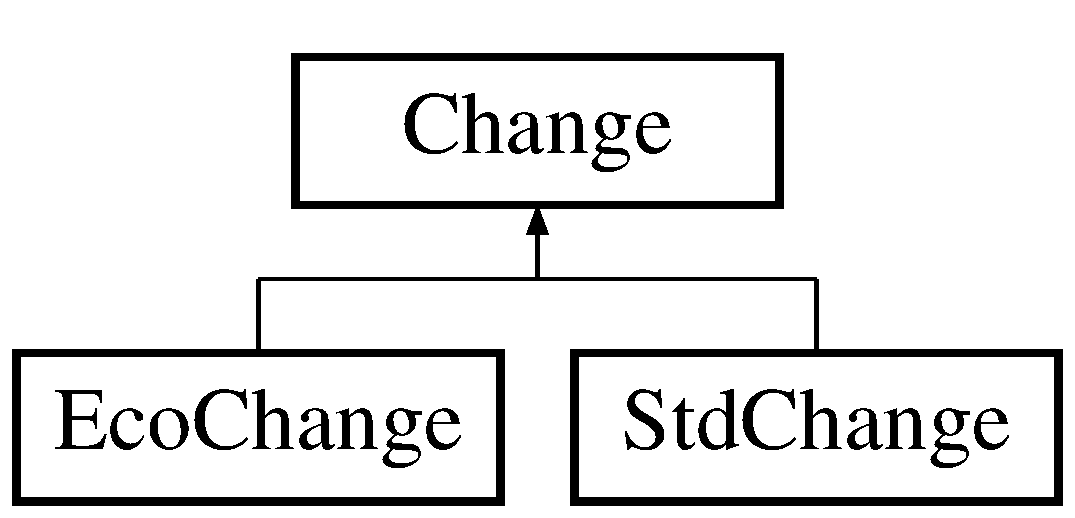
\includegraphics[height=2.000000cm]{classChange}
\end{center}
\end{figure}
\subsection*{Public Member Functions}
\begin{DoxyCompactItemize}
\item 
virtual double \hyperlink{classChange_a59b9108e42a0aef74f735c1f82d4f014}{get\+Change} (\hyperlink{classSpecies}{Species} $\ast$spec, double delta, vector$<$ unique\+\_\+ptr$<$ \hyperlink{classSpecies}{Species} $>$$>$ $\ast$species\+List)=0
\begin{DoxyCompactList}\small\item\em Method to calculate change in species density. \end{DoxyCompactList}\end{DoxyCompactItemize}


\subsection{Detailed Description}
Class containing just one function, used to calculate change in species density (virtual). 

The \hyperlink{classChange}{Change} class has no attributes and only one method, used to calculate change in species density. For now, there are only two implemented versions of that method, with and without taking the environmental constant and species optimum into account (\hyperlink{classEcoChange}{Eco\+Change} and \hyperlink{classStdChange}{Std\+Change}). 

\subsection{Member Function Documentation}
\hypertarget{classChange_a59b9108e42a0aef74f735c1f82d4f014}{}\label{classChange_a59b9108e42a0aef74f735c1f82d4f014} 
\index{Change@{Change}!get\+Change@{get\+Change}}
\index{get\+Change@{get\+Change}!Change@{Change}}
\subsubsection{\texorpdfstring{get\+Change()}{getChange()}}
{\footnotesize\ttfamily virtual double Change\+::get\+Change (\begin{DoxyParamCaption}\item[{\hyperlink{classSpecies}{Species} $\ast$}]{spec,  }\item[{double}]{delta,  }\item[{vector$<$ unique\+\_\+ptr$<$ \hyperlink{classSpecies}{Species} $>$$>$ $\ast$}]{species\+List }\end{DoxyParamCaption})\hspace{0.3cm}{\ttfamily [pure virtual]}}



Method to calculate change in species density. 

This method uses the explicit Euler scheme to resolve a Lotka-\/\+Volterra-\/like differential equation we use to calculate the evolution of the system. 
\begin{DoxyParams}{Parameters}
{\em spec} & \hyperlink{classSpecies}{Species} for which we will calculate change in density. \\
\hline
{\em delta} & size of step used in explicit Euler. \\
\hline
{\em species\+List} & List containing all (alive) species present in the environment. \\
\hline
\end{DoxyParams}


Implemented in \hyperlink{classStdChange_a25fd1a3828d026e902bae809278c6dbc}{Std\+Change}, and \hyperlink{classEcoChange_a963a6e9a77b2c7df7cf25bb8931dbe5c}{Eco\+Change}.



The documentation for this class was generated from the following file\+:\begin{DoxyCompactItemize}
\item 
\hyperlink{Change_8hpp}{Change.\+hpp}\end{DoxyCompactItemize}

\hypertarget{classE2MSimulation}{}\section{E2\+M\+Simulation Class Reference}
\label{classE2MSimulation}\index{E2\+M\+Simulation@{E2\+M\+Simulation}}


Class containing all \hyperlink{classEnvironment}{Environment} objects, as well control-\/flow attributes for the simulation.  




{\ttfamily \#include $<$E2\+M\+Simulation.\+hpp$>$}

Inheritance diagram for E2\+M\+Simulation\+:\begin{figure}[H]
\begin{center}
\leavevmode
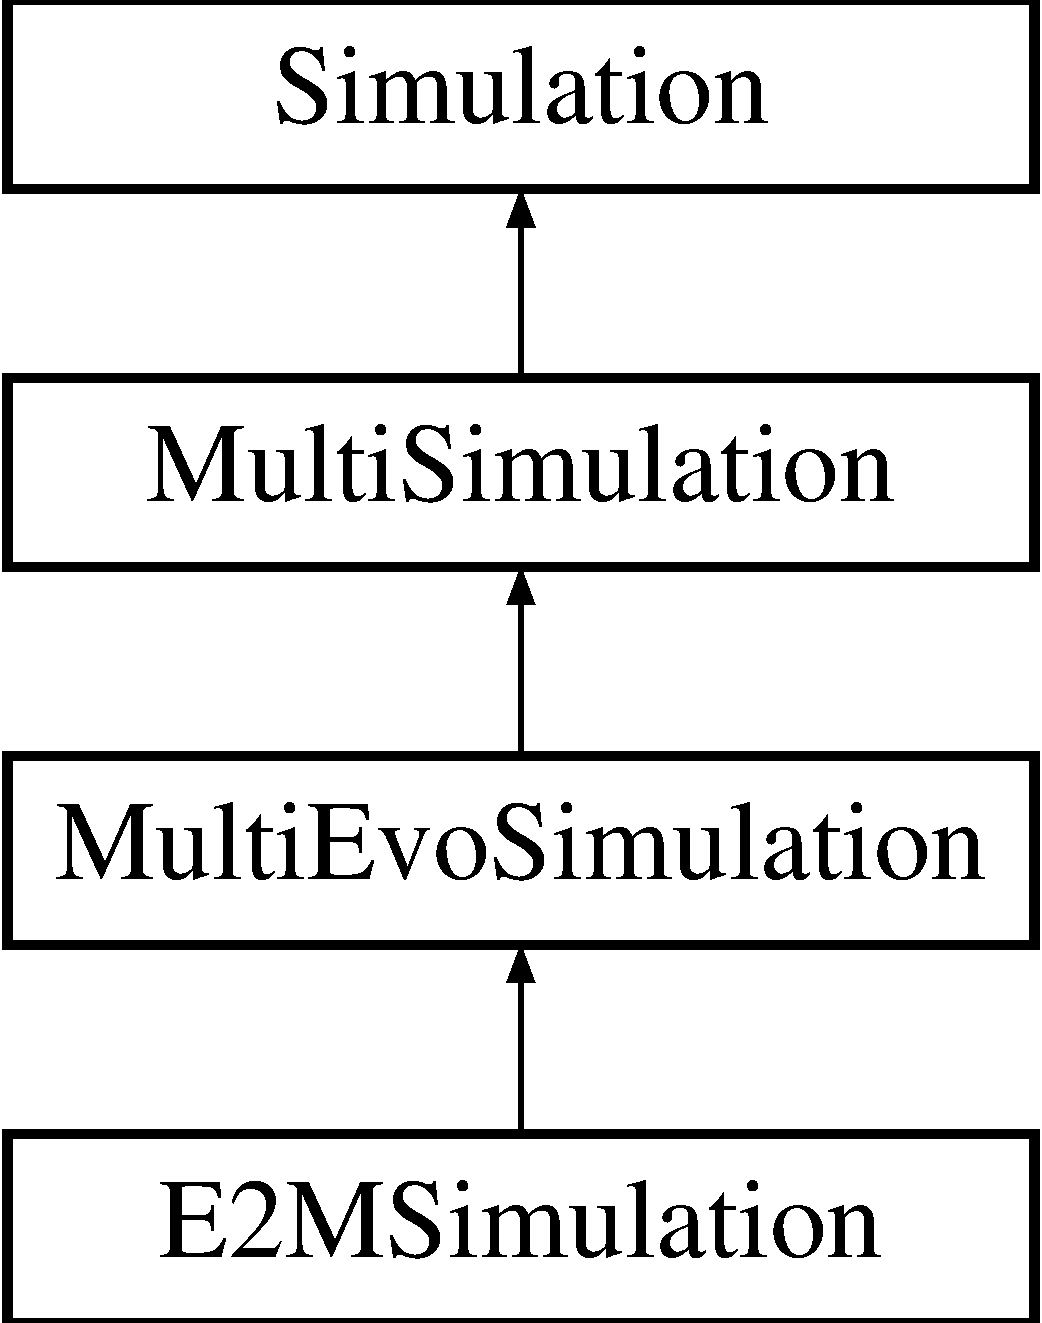
\includegraphics[height=4.000000cm]{classE2MSimulation}
\end{center}
\end{figure}
\subsection*{Public Member Functions}
\begin{DoxyCompactItemize}
\item 
\hypertarget{classE2MSimulation_addbbeb65c91d569a20ddd01ff251fb05}{}\label{classE2MSimulation_addbbeb65c91d569a20ddd01ff251fb05} 
{\bfseries E2\+M\+Simulation} (vector$<$ \hyperlink{classEnvironment}{Environment} $>$ \+\_\+envs)
\item 
\hypertarget{classE2MSimulation_afbbbc3eb05c8e6a9f88c906a95c33ffd}{}\label{classE2MSimulation_afbbbc3eb05c8e6a9f88c906a95c33ffd} 
vector$<$ \hyperlink{classEnvironment}{Environment} $>$ $\ast$ {\bfseries get\+Envs} ()
\item 
\hypertarget{classE2MSimulation_a9fc625c0e66768b4b70cc2b682a3316a}{}\label{classE2MSimulation_a9fc625c0e66768b4b70cc2b682a3316a} 
void {\bfseries set\+Envs} (vector$<$ \hyperlink{classEnvironment}{Environment} $>$ new\+Val)
\item 
\hypertarget{classE2MSimulation_a3cc272d636e0ce6cec2a55cc5cd7970d}{}\label{classE2MSimulation_a3cc272d636e0ce6cec2a55cc5cd7970d} 
void {\bfseries add\+Env} (\hyperlink{classEnvironment}{Environment} env)
\item 
\hypertarget{classE2MSimulation_a433cdd06ccf6fce0636e9c05a1f6eb3a}{}\label{classE2MSimulation_a433cdd06ccf6fce0636e9c05a1f6eb3a} 
void {\bfseries set\+Num\+Envs} (int new\+Val)
\item 
\hypertarget{classE2MSimulation_a04040a96efb80654c6ab3d71c55e43df}{}\label{classE2MSimulation_a04040a96efb80654c6ab3d71c55e43df} 
int {\bfseries get\+Num\+Envs} ()
\item 
\hypertarget{classE2MSimulation_a08698e0fb7b4be7f1e9369aeeec85ca2}{}\label{classE2MSimulation_a08698e0fb7b4be7f1e9369aeeec85ca2} 
void {\bfseries set\+Num\+Specs} (int new\+Val)
\item 
\hypertarget{classE2MSimulation_a113e3427b21a4a6151026d35dc258110}{}\label{classE2MSimulation_a113e3427b21a4a6151026d35dc258110} 
int {\bfseries get\+Num\+Specs} ()
\item 
int \hyperlink{classE2MSimulation_aeac4e92c10f89a5c953ace5b1327d20b}{run\+Sim} (int run\+Number)
\begin{DoxyCompactList}\small\item\em Method that runs the main loop of the simulation. \end{DoxyCompactList}\end{DoxyCompactItemize}
\subsection*{Protected Attributes}
\begin{DoxyCompactItemize}
\item 
\hypertarget{classE2MSimulation_ae77494b8c30893e459c995f95f671e4b}{}\label{classE2MSimulation_ae77494b8c30893e459c995f95f671e4b} 
vector$<$ \hyperlink{classEnvironment}{Environment} $>$ {\bfseries envs}
\end{DoxyCompactItemize}


\subsection{Detailed Description}
Class containing all \hyperlink{classEnvironment}{Environment} objects, as well control-\/flow attributes for the simulation. 

Same as \hyperlink{classE2Simulation}{E2\+Simulation}, but for simulations with multiple environments (see also \hyperlink{classMultiSimulation}{Multi\+Simulation}) 

\subsection{Member Function Documentation}
\hypertarget{classE2MSimulation_aeac4e92c10f89a5c953ace5b1327d20b}{}\label{classE2MSimulation_aeac4e92c10f89a5c953ace5b1327d20b} 
\index{E2\+M\+Simulation@{E2\+M\+Simulation}!run\+Sim@{run\+Sim}}
\index{run\+Sim@{run\+Sim}!E2\+M\+Simulation@{E2\+M\+Simulation}}
\subsubsection{\texorpdfstring{run\+Sim()}{runSim()}}
{\footnotesize\ttfamily int E2\+M\+Simulation\+::run\+Sim (\begin{DoxyParamCaption}\item[{int}]{run\+Number }\end{DoxyParamCaption})\hspace{0.3cm}{\ttfamily [virtual]}}



Method that runs the main loop of the simulation. 


\begin{DoxyParams}{Parameters}
{\em run\+Number} & ID of the current run of the simulation. \\
\hline
\end{DoxyParams}


Reimplemented from \hyperlink{classMultiEvoSimulation_a89c9806ac998c06230cdd41cc6a532bf}{Multi\+Evo\+Simulation}.



The documentation for this class was generated from the following files\+:\begin{DoxyCompactItemize}
\item 
\hyperlink{E2MSimulation_8hpp}{E2\+M\+Simulation.\+hpp}\item 
E2\+M\+Simulation.\+cpp\end{DoxyCompactItemize}

\hypertarget{classE2MultiNextGen}{}\section{E2\+Multi\+Next\+Gen Class Reference}
\label{classE2MultiNextGen}\index{E2\+Multi\+Next\+Gen@{E2\+Multi\+Next\+Gen}}


Class containing a single method, used to control transition from one step to the next, and update Species/\+Environemnt attributes.  




{\ttfamily \#include $<$E2\+Multi\+Next\+Gen.\+hpp$>$}

Inheritance diagram for E2\+Multi\+Next\+Gen\+:\begin{figure}[H]
\begin{center}
\leavevmode
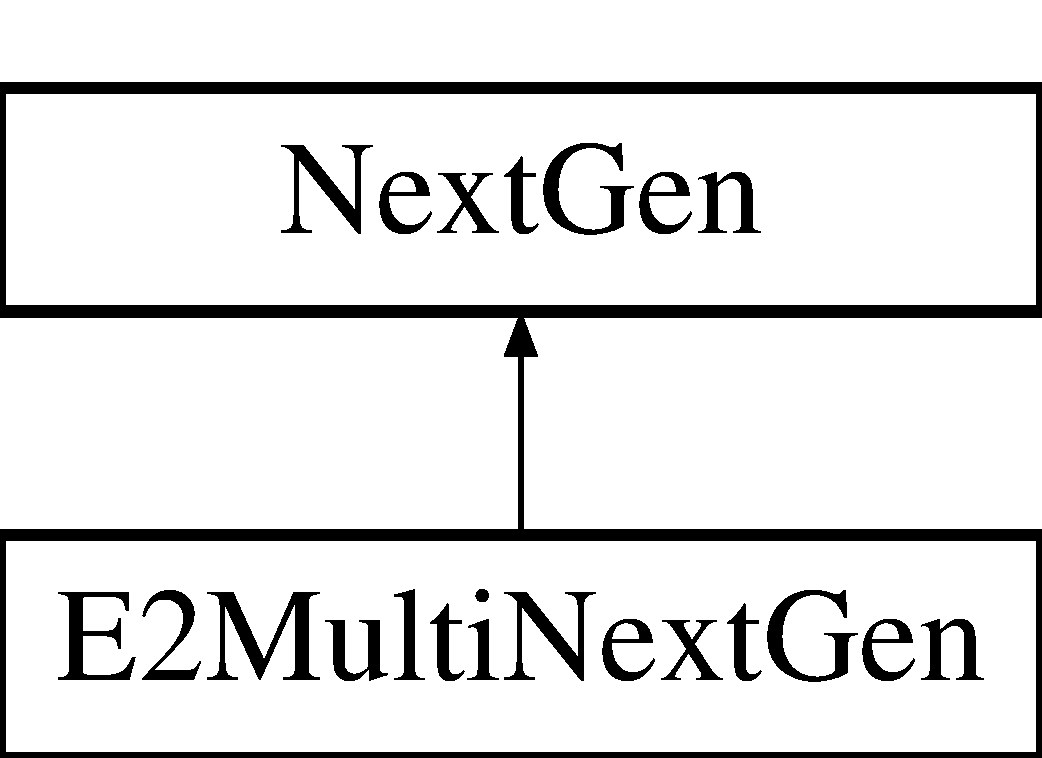
\includegraphics[height=2.000000cm]{classE2MultiNextGen}
\end{center}
\end{figure}
\subsection*{Public Member Functions}
\begin{DoxyCompactItemize}
\item 
void \hyperlink{classE2MultiNextGen_a22721fa0e9c2cbe1de3d0d6bb78932f0}{get\+Next\+Gen} (int step\+Num, std\+::vector$<$ std\+::unique\+\_\+ptr$<$ \hyperlink{classSpecies}{Species} $>$$>$ $\ast$species\+List, \hyperlink{classEnvironment}{Environment} $\ast$env)
\begin{DoxyCompactList}\small\item\em Method used to update \hyperlink{classSpecies}{Species} density at each timestep. \end{DoxyCompactList}\end{DoxyCompactItemize}


\subsection{Detailed Description}
Class containing a single method, used to control transition from one step to the next, and update Species/\+Environemnt attributes. 

\subsection{Member Function Documentation}
\mbox{\Hypertarget{classE2MultiNextGen_a22721fa0e9c2cbe1de3d0d6bb78932f0}\label{classE2MultiNextGen_a22721fa0e9c2cbe1de3d0d6bb78932f0}} 
\index{E2\+Multi\+Next\+Gen@{E2\+Multi\+Next\+Gen}!get\+Next\+Gen@{get\+Next\+Gen}}
\index{get\+Next\+Gen@{get\+Next\+Gen}!E2\+Multi\+Next\+Gen@{E2\+Multi\+Next\+Gen}}
\subsubsection{\texorpdfstring{get\+Next\+Gen()}{getNextGen()}}
{\footnotesize\ttfamily void E2\+Multi\+Next\+Gen\+::get\+Next\+Gen (\begin{DoxyParamCaption}\item[{int}]{step\+Num,  }\item[{std\+::vector$<$ std\+::unique\+\_\+ptr$<$ \hyperlink{classSpecies}{Species} $>$$>$ $\ast$}]{species\+List,  }\item[{\hyperlink{classEnvironment}{Environment} $\ast$}]{env }\end{DoxyParamCaption})\hspace{0.3cm}{\ttfamily [virtual]}}



Method used to update \hyperlink{classSpecies}{Species} density at each timestep. 

This method works exactly like the one in \hyperlink{classE2NextGen}{E2\+Next\+Gen}, except that species with {\ttfamily density == 0} are not moved to env.\+dead\+Species, to avoid having to recreate them if a population from said species migrates into environment from somewhere. If migration probability is very low for all species, it might be worth to delete/introduce them each time, since this might take less time than the increased loop time caused by a higher number of species (I\textquotesingle{}d say it depends on the simulation parameters, but I haven\textquotesingle{}t done any performance tests to compare the two methods).


\begin{DoxyParams}{Parameters}
{\em step\+Num} & Values of the current step \\
\hline
{\em species\+List} & List containing all \hyperlink{classSpecies}{Species} of the environment \\
\hline
{\em env} & Pointer to current environment \\
\hline
\end{DoxyParams}


Implements \hyperlink{classNextGen_aa70da77e0ac03da1bd5414c5e3fd70c0}{Next\+Gen}.



The documentation for this class was generated from the following files\+:\begin{DoxyCompactItemize}
\item 
\hyperlink{E2MultiNextGen_8hpp}{E2\+Multi\+Next\+Gen.\+hpp}\item 
E2\+Multi\+Next\+Gen.\+cpp\end{DoxyCompactItemize}

\hypertarget{classE2NextGen}{}\section{E2\+Next\+Gen Class Reference}
\label{classE2NextGen}\index{E2\+Next\+Gen@{E2\+Next\+Gen}}


Class containing a single method, used to control transition from one step to the next, and update Species/\+Environemnt attributes.  




{\ttfamily \#include $<$E2\+Next\+Gen.\+hpp$>$}

Inheritance diagram for E2\+Next\+Gen\+:\begin{figure}[H]
\begin{center}
\leavevmode
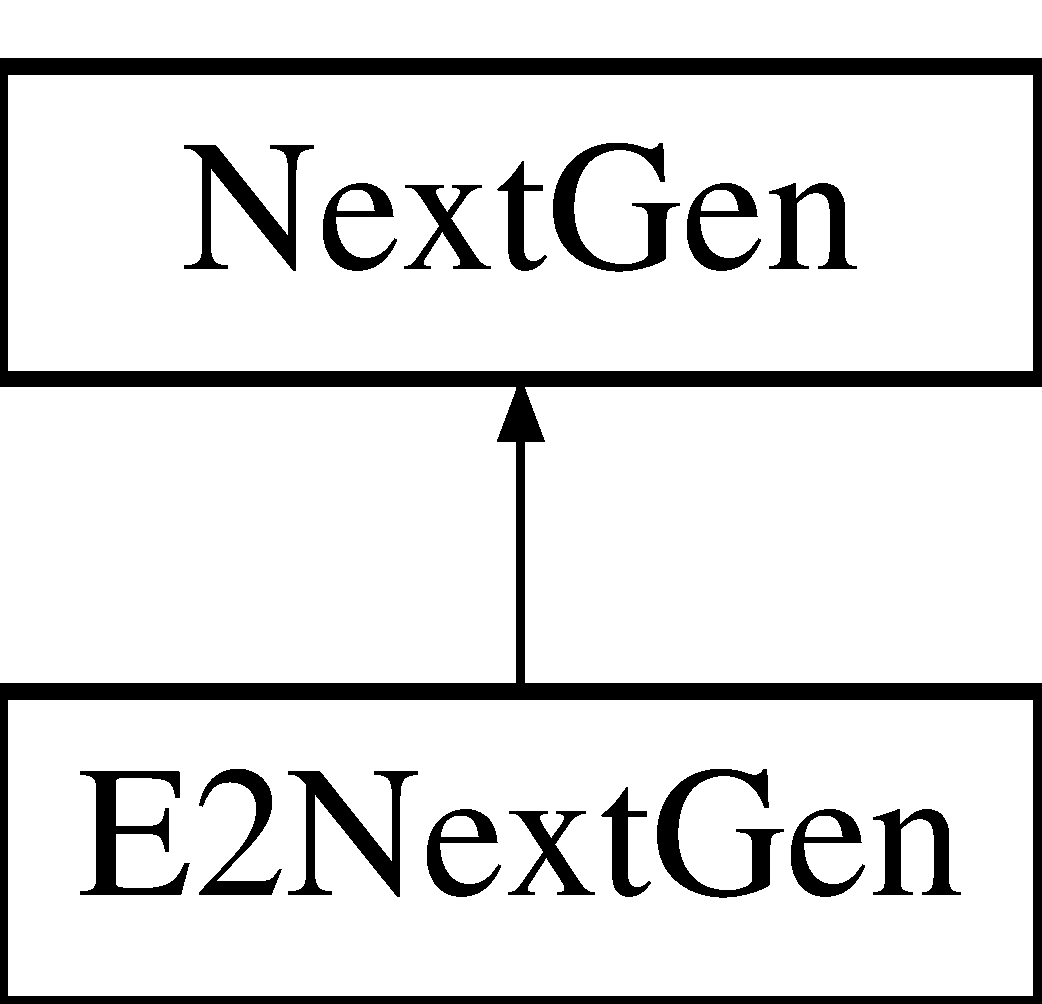
\includegraphics[height=2.000000cm]{classE2NextGen}
\end{center}
\end{figure}
\subsection*{Public Member Functions}
\begin{DoxyCompactItemize}
\item 
void \hyperlink{classE2NextGen_a2c5d35d9c8f9395cbd58d8fb837a08da}{get\+Next\+Gen} (int step\+Num, std\+::vector$<$ std\+::unique\+\_\+ptr$<$ \hyperlink{classSpecies}{Species} $>$$>$ $\ast$species\+List, \hyperlink{classEnvironment}{Environment} $\ast$env)
\begin{DoxyCompactList}\small\item\em Method used to update \hyperlink{classSpecies}{Species} density and interactions, as wel as environmental constant at each timestep. \end{DoxyCompactList}\end{DoxyCompactItemize}


\subsection{Detailed Description}
Class containing a single method, used to control transition from one step to the next, and update Species/\+Environemnt attributes. 

\subsection{Member Function Documentation}
\hypertarget{classE2NextGen_a2c5d35d9c8f9395cbd58d8fb837a08da}{}\label{classE2NextGen_a2c5d35d9c8f9395cbd58d8fb837a08da} 
\index{E2\+Next\+Gen@{E2\+Next\+Gen}!get\+Next\+Gen@{get\+Next\+Gen}}
\index{get\+Next\+Gen@{get\+Next\+Gen}!E2\+Next\+Gen@{E2\+Next\+Gen}}
\subsubsection{\texorpdfstring{get\+Next\+Gen()}{getNextGen()}}
{\footnotesize\ttfamily void E2\+Next\+Gen\+::get\+Next\+Gen (\begin{DoxyParamCaption}\item[{int}]{step\+Num,  }\item[{std\+::vector$<$ std\+::unique\+\_\+ptr$<$ \hyperlink{classSpecies}{Species} $>$$>$ $\ast$}]{species\+List,  }\item[{\hyperlink{classEnvironment}{Environment} $\ast$}]{env }\end{DoxyParamCaption})\hspace{0.3cm}{\ttfamily [virtual]}}



Method used to update \hyperlink{classSpecies}{Species} density and interactions, as wel as environmental constant at each timestep. 

This method works much in the same way as that of \hyperlink{classStdNextGen}{Std\+Next\+Gen}, but with the added functionality of both \hyperlink{classEcoNextGen}{Eco\+Next\+Gen} and \hyperlink{classEvoNextGen}{Evo\+Next\+Gen}.


\begin{DoxyParams}{Parameters}
{\em step\+Num} & Values of the current step \\
\hline
{\em species\+List} & List containing all \hyperlink{classSpecies}{Species} of the environment \\
\hline
{\em env} & Pointer to current environment \\
\hline
\end{DoxyParams}


Implements \hyperlink{classNextGen_aa70da77e0ac03da1bd5414c5e3fd70c0}{Next\+Gen}.



The documentation for this class was generated from the following files\+:\begin{DoxyCompactItemize}
\item 
\hyperlink{E2NextGen_8hpp}{E2\+Next\+Gen.\+hpp}\item 
E2\+Next\+Gen.\+cpp\end{DoxyCompactItemize}

\hypertarget{classE2Simulation}{}\section{E2\+Simulation Class Reference}
\label{classE2Simulation}\index{E2\+Simulation@{E2\+Simulation}}


Class containing all \hyperlink{classEnvironment}{Environment} objects, as well control-\/flow attributes for the simulation.  




{\ttfamily \#include $<$E2\+Simulation.\+hpp$>$}

Inheritance diagram for E2\+Simulation\+:\begin{figure}[H]
\begin{center}
\leavevmode
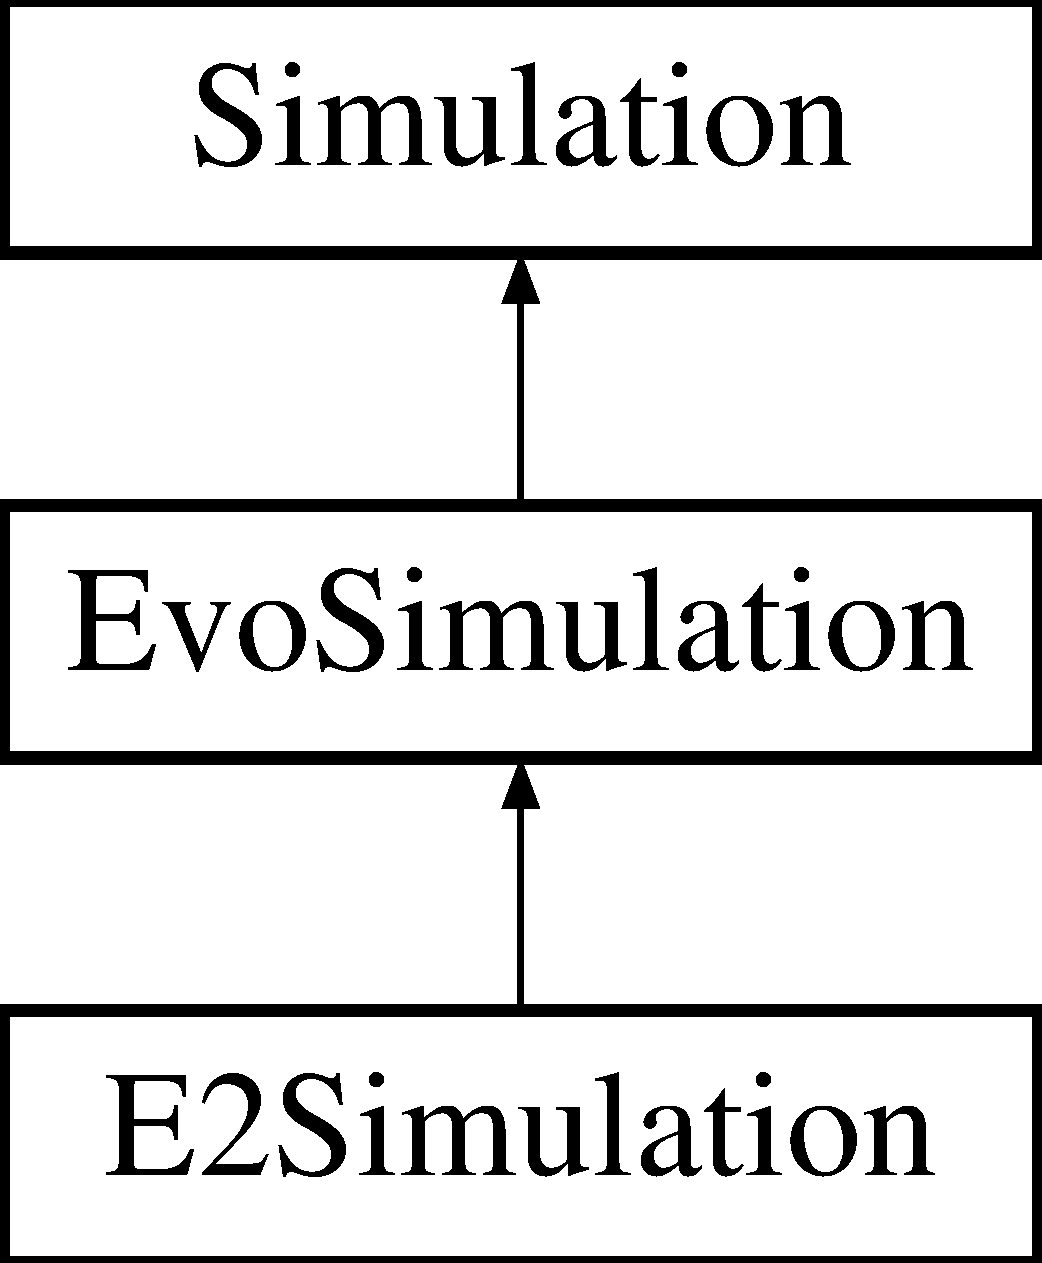
\includegraphics[height=3.000000cm]{classE2Simulation}
\end{center}
\end{figure}
\subsection*{Public Member Functions}
\begin{DoxyCompactItemize}
\item 
\mbox{\Hypertarget{classE2Simulation_a489002277b77dde3163f335eeb174a9c}\label{classE2Simulation_a489002277b77dde3163f335eeb174a9c}} 
{\bfseries E2\+Simulation} (vector$<$ \hyperlink{classEnvironment}{Environment} $>$ \+\_\+env)
\item 
\mbox{\Hypertarget{classE2Simulation_aa814d76fc89318c950e936ba98adad7c}\label{classE2Simulation_aa814d76fc89318c950e936ba98adad7c}} 
int {\bfseries get\+Inter\+Save\+Div} ()
\item 
\mbox{\Hypertarget{classE2Simulation_a440ebe2b5d56c6c3c7d67e6463347752}\label{classE2Simulation_a440ebe2b5d56c6c3c7d67e6463347752}} 
void {\bfseries set\+Inter\+Save\+Div} (int new\+Val)
\item 
\mbox{\Hypertarget{classE2Simulation_a5f07ce9232d20974595ea8191fb93bfe}\label{classE2Simulation_a5f07ce9232d20974595ea8191fb93bfe}} 
vector$<$ \hyperlink{classEnvironment}{Environment} $>$ $\ast$ {\bfseries get\+Envs} ()
\item 
\mbox{\Hypertarget{classE2Simulation_ad7ce5318a2850d7a73df94aec1c7e15f}\label{classE2Simulation_ad7ce5318a2850d7a73df94aec1c7e15f}} 
void {\bfseries add\+Env} (\hyperlink{classEnvironment}{Environment} new\+Val)
\item 
int \hyperlink{classE2Simulation_a28028881fd443d2445b562512cb2169c}{run\+Sim} (int run\+Number)
\begin{DoxyCompactList}\small\item\em Method that runs the main loop of the simulation. \end{DoxyCompactList}\end{DoxyCompactItemize}
\subsection*{Protected Attributes}
\begin{DoxyCompactItemize}
\item 
\mbox{\Hypertarget{classE2Simulation_a72c3fa1a40648aeb904c6afb74dbb700}\label{classE2Simulation_a72c3fa1a40648aeb904c6afb74dbb700}} 
vector$<$ \hyperlink{classEnvironment}{Environment} $>$ {\bfseries envs}
\end{DoxyCompactItemize}


\subsection{Detailed Description}
Class containing all \hyperlink{classEnvironment}{Environment} objects, as well control-\/flow attributes for the simulation. 

The E2\+Simulaiton class is very similar to the simulation class, except that it has the extra functionality of both \hyperlink{classEcoSimulation}{Eco\+Simulation} and \hyperlink{classEvoSimulation}{Evo\+Simulation}. 

\subsection{Member Function Documentation}
\mbox{\Hypertarget{classE2Simulation_a28028881fd443d2445b562512cb2169c}\label{classE2Simulation_a28028881fd443d2445b562512cb2169c}} 
\index{E2\+Simulation@{E2\+Simulation}!run\+Sim@{run\+Sim}}
\index{run\+Sim@{run\+Sim}!E2\+Simulation@{E2\+Simulation}}
\subsubsection{\texorpdfstring{run\+Sim()}{runSim()}}
{\footnotesize\ttfamily int E2\+Simulation\+::run\+Sim (\begin{DoxyParamCaption}\item[{int}]{run\+Number }\end{DoxyParamCaption})\hspace{0.3cm}{\ttfamily [virtual]}}



Method that runs the main loop of the simulation. 


\begin{DoxyParams}{Parameters}
{\em run\+Number} & ID of the current run of the simulation. \\
\hline
\end{DoxyParams}


Reimplemented from \hyperlink{classEvoSimulation_aa43aa351dec24c638e56995a67a4f0f5}{Evo\+Simulation}.



The documentation for this class was generated from the following files\+:\begin{DoxyCompactItemize}
\item 
\hyperlink{E2Simulation_8hpp}{E2\+Simulation.\+hpp}\item 
E2\+Simulation.\+cpp\end{DoxyCompactItemize}

\hypertarget{classEcoChange}{}\section{Eco\+Change Class Reference}
\label{classEcoChange}\index{Eco\+Change@{Eco\+Change}}


Class containing just one function, used to calculate change in species density.  




{\ttfamily \#include $<$Eco\+Change.\+hpp$>$}

Inheritance diagram for Eco\+Change\+:\begin{figure}[H]
\begin{center}
\leavevmode
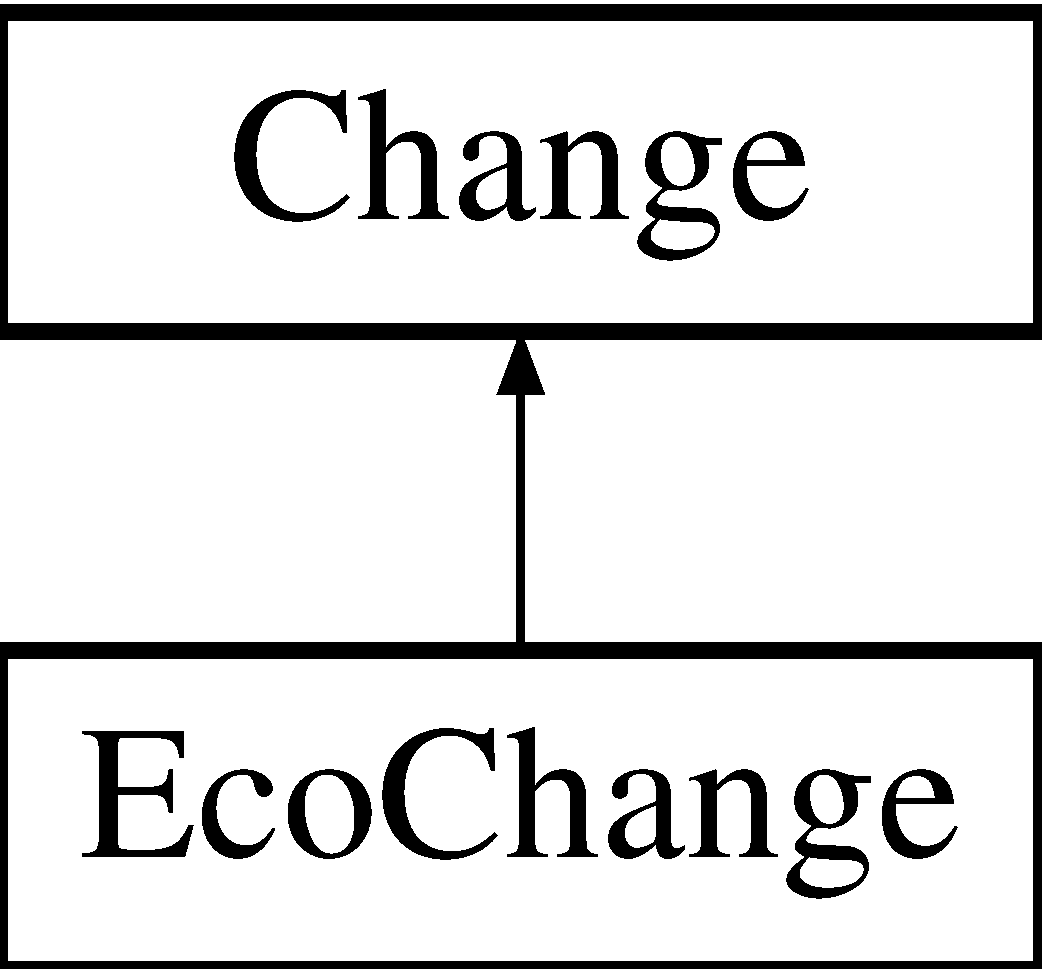
\includegraphics[height=2.000000cm]{classEcoChange}
\end{center}
\end{figure}
\subsection*{Public Member Functions}
\begin{DoxyCompactItemize}
\item 
double \hyperlink{classEcoChange_a963a6e9a77b2c7df7cf25bb8931dbe5c}{get\+Change} (\hyperlink{classSpecies}{Species} $\ast$spec, double delta, vector$<$ unique\+\_\+ptr$<$ \hyperlink{classSpecies}{Species} $>$$>$ $\ast$species\+List)
\begin{DoxyCompactList}\small\item\em Method to calculate change in species density. \end{DoxyCompactList}\end{DoxyCompactItemize}


\subsection{Detailed Description}
Class containing just one function, used to calculate change in species density. 

The \hyperlink{classEcoChange}{Eco\+Change} class calculates change in species density taking the environmental constant and species optimum into account. The same formula as in \hyperlink{classStdChange}{Std\+Change} is used (not inherited since it is very little code and we want to keep the calling stack to a minimum for performance). However, if change is positive (species density is increasing), it is modified by\+:

$ \dot{x_i} = \dot{x_i} * e^{-(envConst - opt)^2}$ 

\subsection{Member Function Documentation}
\hypertarget{classEcoChange_a963a6e9a77b2c7df7cf25bb8931dbe5c}{}\label{classEcoChange_a963a6e9a77b2c7df7cf25bb8931dbe5c} 
\index{Eco\+Change@{Eco\+Change}!get\+Change@{get\+Change}}
\index{get\+Change@{get\+Change}!Eco\+Change@{Eco\+Change}}
\subsubsection{\texorpdfstring{get\+Change()}{getChange()}}
{\footnotesize\ttfamily double Eco\+Change\+::get\+Change (\begin{DoxyParamCaption}\item[{\hyperlink{classSpecies}{Species} $\ast$}]{spec,  }\item[{double}]{delta,  }\item[{vector$<$ unique\+\_\+ptr$<$ \hyperlink{classSpecies}{Species} $>$$>$ $\ast$}]{species\+List }\end{DoxyParamCaption})\hspace{0.3cm}{\ttfamily [virtual]}}



Method to calculate change in species density. 

This method uses the explicit Euler scheme to resolve a Lotka-\/\+Volterra-\/like differential equation we use to calculate the evolution of the system. 
\begin{DoxyParams}{Parameters}
{\em spec} & \hyperlink{classSpecies}{Species} for which we will calculate change in density. \\
\hline
{\em delta} & size of step used in explicit Euler. \\
\hline
{\em species\+List} & List containing all (alive) species present in the environment. \\
\hline
\end{DoxyParams}


Implements \hyperlink{classChange_a59b9108e42a0aef74f735c1f82d4f014}{Change}.



The documentation for this class was generated from the following files\+:\begin{DoxyCompactItemize}
\item 
\hyperlink{EcoChange_8hpp}{Eco\+Change.\+hpp}\item 
Eco\+Change.\+cpp\end{DoxyCompactItemize}

\hypertarget{classEcoEvo}{}\section{Eco\+Evo Class Reference}
\label{classEcoEvo}\index{Eco\+Evo@{Eco\+Evo}}


Implementation of the \hyperlink{classEvo}{Evo} class that acts on species optimum as well as interactions.  




{\ttfamily \#include $<$Eco\+Evo.\+hpp$>$}

Inheritance diagram for Eco\+Evo\+:\begin{figure}[H]
\begin{center}
\leavevmode
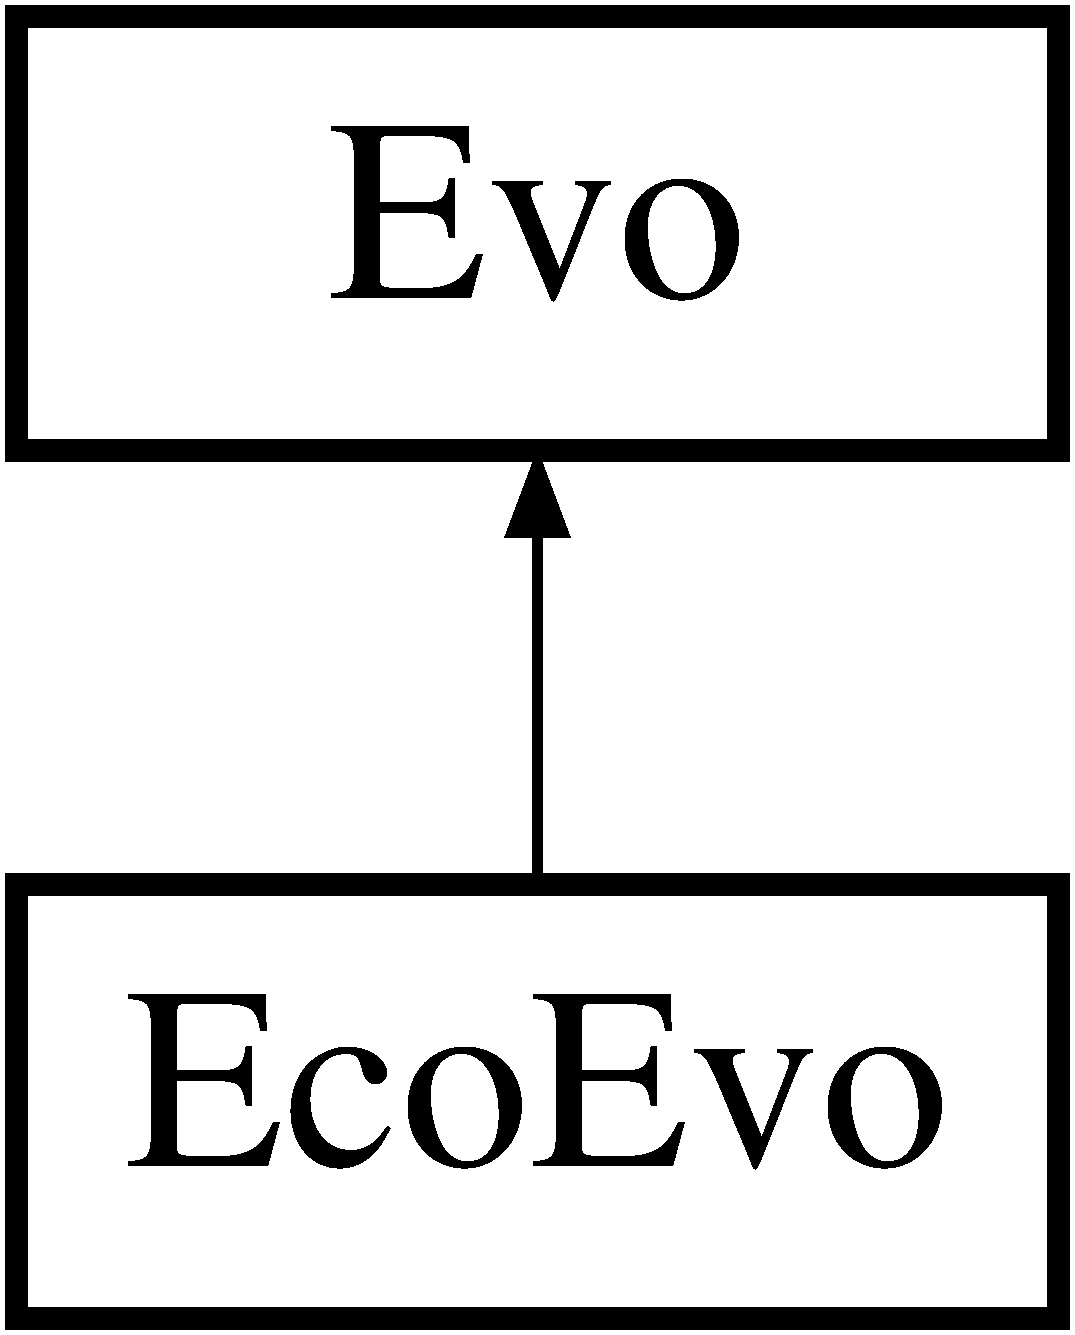
\includegraphics[height=2.000000cm]{classEcoEvo}
\end{center}
\end{figure}
\subsection*{Public Member Functions}
\begin{DoxyCompactItemize}
\item 
void \hyperlink{classEcoEvo_a93564a6d93cdc1802182273c353e0552}{get\+Evo} (vector$<$ unique\+\_\+ptr$<$ \hyperlink{classSpecies}{Species} $>$$>$ $\ast$species\+List, \hyperlink{classSpecies}{Species} $\ast$spec, int resolution)
\begin{DoxyCompactList}\small\item\em Controller method for updating species interactions/optimum. \end{DoxyCompactList}\item 
vector$<$ unique\+\_\+ptr$<$ \hyperlink{classIndividual}{Individual} $>$ $>$ \hyperlink{classEcoEvo_a819363c533784efea949ebc70a6d4636}{get\+Inds} (vector$<$ unique\+\_\+ptr$<$ \hyperlink{classSpecies}{Species} $>$$>$ $\ast$species\+List, \hyperlink{classSpecies}{Species} $\ast$spec, int resolution)
\begin{DoxyCompactList}\small\item\em Method for creating individuals from species. \end{DoxyCompactList}\item 
vector$<$ int $>$ \hyperlink{classEcoEvo_adfd00eb377489649a279e567abc3ae94}{run\+Selection} (vector$<$ unique\+\_\+ptr$<$ \hyperlink{classIndividual}{Individual} $>$$>$ $\ast$inds, vector$<$ unique\+\_\+ptr$<$ \hyperlink{classSpecies}{Species} $>$$>$ $\ast$species\+List)
\begin{DoxyCompactList}\small\item\em Method that selects surviving/reproducing individuals. \end{DoxyCompactList}\end{DoxyCompactItemize}
\subsection*{Additional Inherited Members}


\subsection{Detailed Description}
Implementation of the \hyperlink{classEvo}{Evo} class that acts on species optimum as well as interactions. 

The \hyperlink{classEcoEvo}{Eco\+Evo} class implements the \hyperlink{classEcoEvo_a819363c533784efea949ebc70a6d4636}{get\+Inds()} method differently from \hyperlink{classStdEvo}{Std\+Evo}, since it creates \hyperlink{classI2}{I2} objects to which it returns a list of pointers. The \hyperlink{classEcoEvo_adfd00eb377489649a279e567abc3ae94}{run\+Selection()} method remains the same, but \hyperlink{classEcoEvo_a93564a6d93cdc1802182273c353e0552}{get\+Evo()} also updates species optimum. 

\subsection{Member Function Documentation}
\mbox{\Hypertarget{classEcoEvo_a93564a6d93cdc1802182273c353e0552}\label{classEcoEvo_a93564a6d93cdc1802182273c353e0552}} 
\index{Eco\+Evo@{Eco\+Evo}!get\+Evo@{get\+Evo}}
\index{get\+Evo@{get\+Evo}!Eco\+Evo@{Eco\+Evo}}
\subsubsection{\texorpdfstring{get\+Evo()}{getEvo()}}
{\footnotesize\ttfamily void Eco\+Evo\+::get\+Evo (\begin{DoxyParamCaption}\item[{vector$<$ unique\+\_\+ptr$<$ \hyperlink{classSpecies}{Species} $>$$>$ $\ast$}]{species\+List,  }\item[{\hyperlink{classSpecies}{Species} $\ast$}]{spec,  }\item[{int}]{resolution }\end{DoxyParamCaption})\hspace{0.3cm}{\ttfamily [virtual]}}



Controller method for updating species interactions/optimum. 

Calls \hyperlink{classEcoEvo_a819363c533784efea949ebc70a6d4636}{get\+Inds()} to get a list of individuals on which to call \hyperlink{classEcoEvo_adfd00eb377489649a279e567abc3ae94}{run\+Selection()}. Then calculates the mean of all interaction values, as well as optimum, from selected individuals, and sets this as the new interaction values, and optimum, for the species.


\begin{DoxyParams}{Parameters}
{\em species\+List} & List containing all (alive) species present in the environment (used to calculate survival/reproduction probability of indivduals). \\
\hline
{\em spec} & \hyperlink{classSpecies}{Species} for which we will calculate evolutionary change (parameters are automatically updated during call). \\
\hline
{\em resolution} & How many discrete individuals are contained in one unit of density. \\
\hline
\end{DoxyParams}


Implements \hyperlink{classEvo_a8c5208c00d1ee2fe9bef41bdd7fe0ab7}{Evo}.

\mbox{\Hypertarget{classEcoEvo_a819363c533784efea949ebc70a6d4636}\label{classEcoEvo_a819363c533784efea949ebc70a6d4636}} 
\index{Eco\+Evo@{Eco\+Evo}!get\+Inds@{get\+Inds}}
\index{get\+Inds@{get\+Inds}!Eco\+Evo@{Eco\+Evo}}
\subsubsection{\texorpdfstring{get\+Inds()}{getInds()}}
{\footnotesize\ttfamily vector$<$ unique\+\_\+ptr$<$ \hyperlink{classIndividual}{Individual} $>$ $>$ Eco\+Evo\+::get\+Inds (\begin{DoxyParamCaption}\item[{vector$<$ unique\+\_\+ptr$<$ \hyperlink{classSpecies}{Species} $>$$>$ $\ast$}]{species\+List,  }\item[{\hyperlink{classSpecies}{Species} $\ast$}]{spec,  }\item[{int}]{resolution }\end{DoxyParamCaption})\hspace{0.3cm}{\ttfamily [virtual]}}



Method for creating individuals from species. 

This method divides a species with continous density into a discrete number of individuals {\ttfamily num\+Inds = round(species.\+density) $\ast$ resolution + 1$<$$>$ (+1 to avoid divide-\/by-\/zero errors). Interaction values for each individual are generated from a gaussian distribution $\mathcal{N}(\mu , \sigma^2)$ where $\mu$ is species interaction value, and $\sigma^2$ is evolution range for that interaction. \hyperlink{classIndividual}{Individual} optimum is calculated in the same manner, with $\mu$ being species optimum, and $\sigma^2$ opt\+Range. Objects pointed to are of class \hyperlink{classI2}{I2} instead of \hyperlink{classIndividual}{Individual} (take environmental constant into account).}

{\ttfamily 
\begin{DoxyParams}{Parameters}
{\em species\+List} & List containing all (alive) species present in the environment (used to calculate survival/reproduction probability of indivduals). \\
\hline
{\em spec} & \hyperlink{classSpecies}{Species} from which we will generate individuals. \\
\hline
{\em resolution} & How many discrete individuals are contained in one unit of density. \\
\hline
\end{DoxyParams}
}

Implements \hyperlink{classEvo_a88b5e0b1053cf1b4b473a08e2f03db92}{Evo}.

\mbox{\Hypertarget{classEcoEvo_adfd00eb377489649a279e567abc3ae94}\label{classEcoEvo_adfd00eb377489649a279e567abc3ae94}} 
\index{Eco\+Evo@{Eco\+Evo}!run\+Selection@{run\+Selection}}
\index{run\+Selection@{run\+Selection}!Eco\+Evo@{Eco\+Evo}}
\subsubsection{\texorpdfstring{run\+Selection()}{runSelection()}}
{\footnotesize\ttfamily vector$<$ int $>$ Eco\+Evo\+::run\+Selection (\begin{DoxyParamCaption}\item[{vector$<$ unique\+\_\+ptr$<$ \hyperlink{classIndividual}{Individual} $>$$>$ $\ast$}]{inds,  }\item[{vector$<$ unique\+\_\+ptr$<$ \hyperlink{classSpecies}{Species} $>$$>$ $\ast$}]{species\+List }\end{DoxyParamCaption})\hspace{0.3cm}{\ttfamily [virtual]}}



Method that selects surviving/reproducing individuals. 

This method calculates survival/reproduction probability for each individual (detailed in the \hyperlink{classI2}{I2} class), and returns a list indicating how many copies of each individual will be in the next generation (either 2 or 0).


\begin{DoxyParams}{Parameters}
{\em inds} & List containing all individuals that were generated from evolving species. \\
\hline
{\em species\+List} & List containing all (alive) species present in the environment (used to calculate survival/reproduction probability of indivduals). \\
\hline
\end{DoxyParams}


Implements \hyperlink{classEvo_a10ff4eefe3967ff5cf5f820890c18079}{Evo}.



The documentation for this class was generated from the following files\+:\begin{DoxyCompactItemize}
\item 
\hyperlink{EcoEvo_8hpp}{Eco\+Evo.\+hpp}\item 
Eco\+Evo.\+cpp\end{DoxyCompactItemize}

\hypertarget{classEcoMultiNextGen}{}\section{Eco\+Multi\+Next\+Gen Class Reference}
\label{classEcoMultiNextGen}\index{Eco\+Multi\+Next\+Gen@{Eco\+Multi\+Next\+Gen}}


Class containing a single method, used to control transition from one step to the next, and update Species/\+Environemnt attributes.  




{\ttfamily \#include $<$Eco\+Multi\+Next\+Gen.\+hpp$>$}

Inheritance diagram for Eco\+Multi\+Next\+Gen\+:\begin{figure}[H]
\begin{center}
\leavevmode
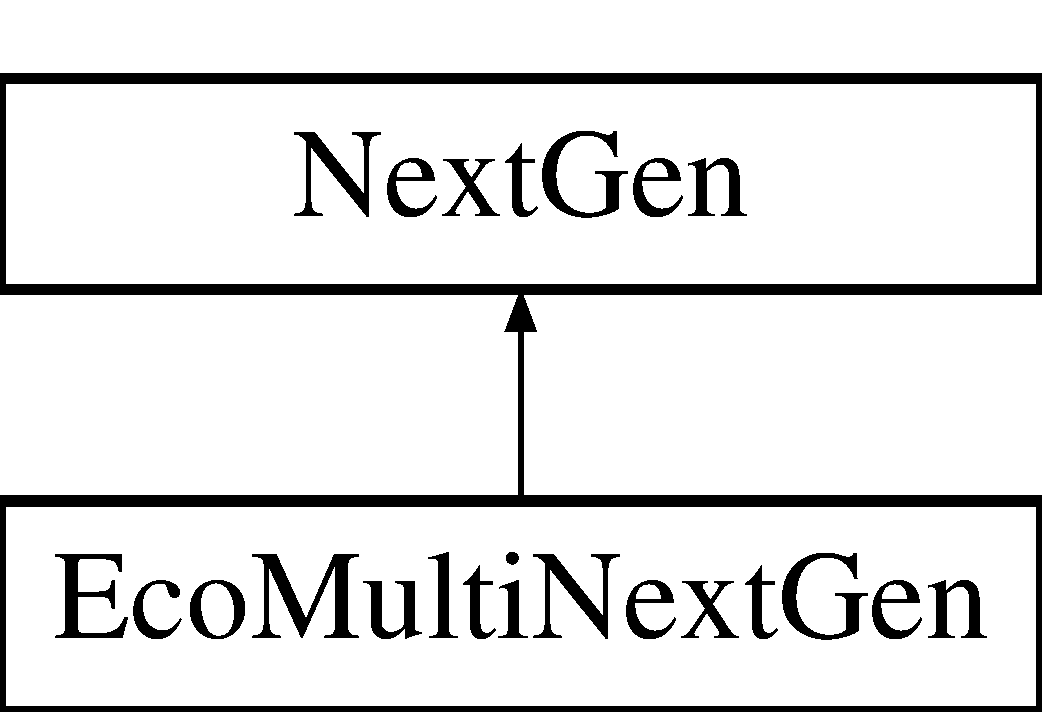
\includegraphics[height=2.000000cm]{classEcoMultiNextGen}
\end{center}
\end{figure}
\subsection*{Public Member Functions}
\begin{DoxyCompactItemize}
\item 
void \hyperlink{classEcoMultiNextGen_a956065141696cac390d8acb8ca5bcccb}{get\+Next\+Gen} (int step\+Num, std\+::vector$<$ std\+::unique\+\_\+ptr$<$ \hyperlink{classSpecies}{Species} $>$$>$ $\ast$species\+List, \hyperlink{classEnvironment}{Environment} $\ast$env)
\begin{DoxyCompactList}\small\item\em Method used to update \hyperlink{classSpecies}{Species} density at each timestep. \end{DoxyCompactList}\end{DoxyCompactItemize}


\subsection{Detailed Description}
Class containing a single method, used to control transition from one step to the next, and update Species/\+Environemnt attributes. 

\subsection{Member Function Documentation}
\mbox{\Hypertarget{classEcoMultiNextGen_a956065141696cac390d8acb8ca5bcccb}\label{classEcoMultiNextGen_a956065141696cac390d8acb8ca5bcccb}} 
\index{Eco\+Multi\+Next\+Gen@{Eco\+Multi\+Next\+Gen}!get\+Next\+Gen@{get\+Next\+Gen}}
\index{get\+Next\+Gen@{get\+Next\+Gen}!Eco\+Multi\+Next\+Gen@{Eco\+Multi\+Next\+Gen}}
\subsubsection{\texorpdfstring{get\+Next\+Gen()}{getNextGen()}}
{\footnotesize\ttfamily void Eco\+Multi\+Next\+Gen\+::get\+Next\+Gen (\begin{DoxyParamCaption}\item[{int}]{step\+Num,  }\item[{std\+::vector$<$ std\+::unique\+\_\+ptr$<$ \hyperlink{classSpecies}{Species} $>$$>$ $\ast$}]{species\+List,  }\item[{\hyperlink{classEnvironment}{Environment} $\ast$}]{env }\end{DoxyParamCaption})\hspace{0.3cm}{\ttfamily [virtual]}}



Method used to update \hyperlink{classSpecies}{Species} density at each timestep. 

This method works exactly like the one in \hyperlink{classEcoNextGen}{Eco\+Next\+Gen}, except that species with {\ttfamily density == 0} are not moved to env.\+dead\+Species, to avoid having to recreate them if a population from said species migrates into environment from somewhere. If migration probability is very low for all species, it might be worth to delete/introduce them each time, since this might take less time than the increased loop time caused by a higher number of species (I\textquotesingle{}d say it depends on the simulation parameters, but I haven\textquotesingle{}t done any performance tests to compare the two methods).


\begin{DoxyParams}{Parameters}
{\em step\+Num} & Values of the current step \\
\hline
{\em species\+List} & List containing all \hyperlink{classSpecies}{Species} of the environment \\
\hline
{\em env} & Pointer to current environment \\
\hline
\end{DoxyParams}


Implements \hyperlink{classNextGen_aa70da77e0ac03da1bd5414c5e3fd70c0}{Next\+Gen}.



The documentation for this class was generated from the following files\+:\begin{DoxyCompactItemize}
\item 
\hyperlink{EcoMultiNextGen_8hpp}{Eco\+Multi\+Next\+Gen.\+hpp}\item 
Eco\+Multi\+Next\+Gen.\+cpp\end{DoxyCompactItemize}

\hypertarget{classEcoNextGen}{}\section{Eco\+Next\+Gen Class Reference}
\label{classEcoNextGen}\index{Eco\+Next\+Gen@{Eco\+Next\+Gen}}


Class containing a single method, used to control transition from one step to the next, and update Species/\+Environemnt attributes.  




{\ttfamily \#include $<$Eco\+Next\+Gen.\+hpp$>$}

Inheritance diagram for Eco\+Next\+Gen\+:\begin{figure}[H]
\begin{center}
\leavevmode
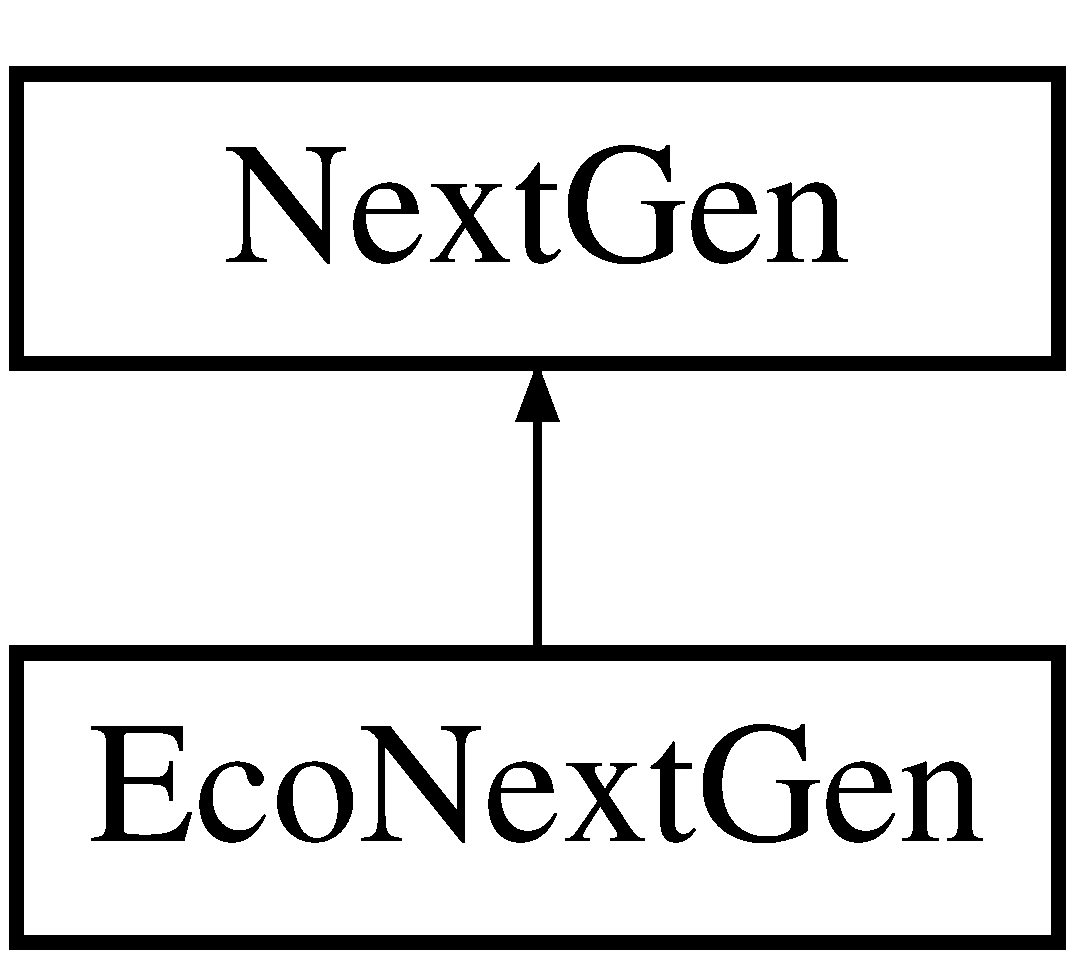
\includegraphics[height=2.000000cm]{classEcoNextGen}
\end{center}
\end{figure}
\subsection*{Public Member Functions}
\begin{DoxyCompactItemize}
\item 
void \hyperlink{classEcoNextGen_a4cb2fccbd3221f41c249c97af461dd3c}{get\+Next\+Gen} (int step\+Num, std\+::vector$<$ std\+::unique\+\_\+ptr$<$ \hyperlink{classSpecies}{Species} $>$$>$ $\ast$species\+List, \hyperlink{classEnvironment}{Environment} $\ast$env)
\begin{DoxyCompactList}\small\item\em Method used to update \hyperlink{classSpecies}{Species} density and environmental constant at each timestep. \end{DoxyCompactList}\end{DoxyCompactItemize}


\subsection{Detailed Description}
Class containing a single method, used to control transition from one step to the next, and update Species/\+Environemnt attributes. 

\subsection{Member Function Documentation}
\mbox{\Hypertarget{classEcoNextGen_a4cb2fccbd3221f41c249c97af461dd3c}\label{classEcoNextGen_a4cb2fccbd3221f41c249c97af461dd3c}} 
\index{Eco\+Next\+Gen@{Eco\+Next\+Gen}!get\+Next\+Gen@{get\+Next\+Gen}}
\index{get\+Next\+Gen@{get\+Next\+Gen}!Eco\+Next\+Gen@{Eco\+Next\+Gen}}
\subsubsection{\texorpdfstring{get\+Next\+Gen()}{getNextGen()}}
{\footnotesize\ttfamily void Eco\+Next\+Gen\+::get\+Next\+Gen (\begin{DoxyParamCaption}\item[{int}]{step\+Num,  }\item[{std\+::vector$<$ std\+::unique\+\_\+ptr$<$ \hyperlink{classSpecies}{Species} $>$$>$ $\ast$}]{species\+List,  }\item[{\hyperlink{classEnvironment}{Environment} $\ast$}]{env }\end{DoxyParamCaption})\hspace{0.3cm}{\ttfamily [virtual]}}



Method used to update \hyperlink{classSpecies}{Species} density and environmental constant at each timestep. 

This method works much in the same way as that of \hyperlink{classStdNextGen}{Std\+Next\+Gen}, except that if a call to get\+Random() (heleprs.\+hpp) returns a value smaller than env.\+pert\+Prob, the environmental constant of env will be changed by a random amount drawn form the uniform distribution (env.\+pert\+Range\mbox{[}0\mbox{]}, env.\+pert\+Range\mbox{[}1\mbox{]}) (this happens before species change in densities are calculated). This perturbation is saved in env.\+perturbations.


\begin{DoxyParams}{Parameters}
{\em step\+Num} & Values of the current step \\
\hline
{\em species\+List} & List containing all \hyperlink{classSpecies}{Species} of the environment \\
\hline
{\em env} & Pointer to current environment \\
\hline
\end{DoxyParams}


Implements \hyperlink{classNextGen_aa70da77e0ac03da1bd5414c5e3fd70c0}{Next\+Gen}.



The documentation for this class was generated from the following files\+:\begin{DoxyCompactItemize}
\item 
\hyperlink{EcoNextGen_8hpp}{Eco\+Next\+Gen.\+hpp}\item 
Eco\+Next\+Gen.\+cpp\end{DoxyCompactItemize}

\hypertarget{classEcoSimulation}{}\section{Eco\+Simulation Class Reference}
\label{classEcoSimulation}\index{Eco\+Simulation@{Eco\+Simulation}}


Class containing all \hyperlink{classEnvironment}{Environment} objects, as well control-\/flow attributes for the simulation.  




{\ttfamily \#include $<$Eco\+Simulation.\+hpp$>$}

Inheritance diagram for Eco\+Simulation\+:\begin{figure}[H]
\begin{center}
\leavevmode
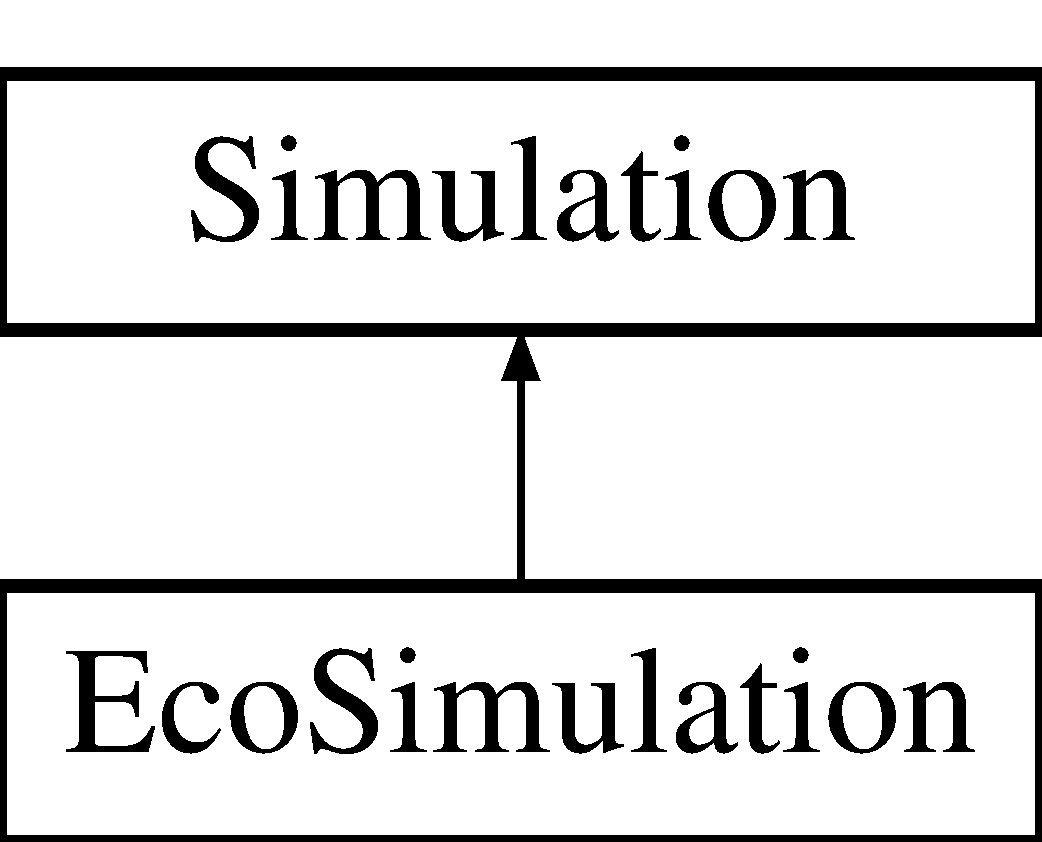
\includegraphics[height=2.000000cm]{classEcoSimulation}
\end{center}
\end{figure}
\subsection*{Public Member Functions}
\begin{DoxyCompactItemize}
\item 
\mbox{\Hypertarget{classEcoSimulation_a25ae3cf6161e29e0934100e61cfbeff2}\label{classEcoSimulation_a25ae3cf6161e29e0934100e61cfbeff2}} 
{\bfseries Eco\+Simulation} (vector$<$ \hyperlink{classEnvironment}{Environment} $>$ \+\_\+env)
\item 
\mbox{\Hypertarget{classEcoSimulation_a36abdefbbb5c3e6e06754f23860b9d8c}\label{classEcoSimulation_a36abdefbbb5c3e6e06754f23860b9d8c}} 
vector$<$ \hyperlink{classEnvironment}{Environment} $>$ $\ast$ {\bfseries get\+Envs} ()
\item 
\mbox{\Hypertarget{classEcoSimulation_a36bafa7e479df22a6ab993f21648817f}\label{classEcoSimulation_a36bafa7e479df22a6ab993f21648817f}} 
void {\bfseries add\+Env} (\hyperlink{classEnvironment}{Environment} new\+Val)
\item 
int \hyperlink{classEcoSimulation_a72ec5e7dffb4231b2cb363b632788622}{run\+Sim} (int run\+Number)
\begin{DoxyCompactList}\small\item\em Method that runs the main loop of the simulation. \end{DoxyCompactList}\end{DoxyCompactItemize}
\subsection*{Additional Inherited Members}


\subsection{Detailed Description}
Class containing all \hyperlink{classEnvironment}{Environment} objects, as well control-\/flow attributes for the simulation. 

The Eco\+Simulaiton class is very similar to the simulation class, except that it also saves all perturbations at the end of a simulation. 

\subsection{Member Function Documentation}
\mbox{\Hypertarget{classEcoSimulation_a72ec5e7dffb4231b2cb363b632788622}\label{classEcoSimulation_a72ec5e7dffb4231b2cb363b632788622}} 
\index{Eco\+Simulation@{Eco\+Simulation}!run\+Sim@{run\+Sim}}
\index{run\+Sim@{run\+Sim}!Eco\+Simulation@{Eco\+Simulation}}
\subsubsection{\texorpdfstring{run\+Sim()}{runSim()}}
{\footnotesize\ttfamily int Eco\+Simulation\+::run\+Sim (\begin{DoxyParamCaption}\item[{int}]{run\+Number }\end{DoxyParamCaption})\hspace{0.3cm}{\ttfamily [virtual]}}



Method that runs the main loop of the simulation. 


\begin{DoxyParams}{Parameters}
{\em run\+Number} & ID of the current run of the simulation. \\
\hline
\end{DoxyParams}


Reimplemented from \hyperlink{classSimulation_a7eb16da89581b496d33b77efbb63b9cd}{Simulation}.



The documentation for this class was generated from the following files\+:\begin{DoxyCompactItemize}
\item 
\hyperlink{EcoSimulation_8hpp}{Eco\+Simulation.\+hpp}\item 
Eco\+Simulation.\+cpp\end{DoxyCompactItemize}

\hypertarget{classEnvironment}{}\section{Environment Class Reference}
\label{classEnvironment}\index{Environment@{Environment}}


Class containing (unique\+\_\+ptrs to) all \hyperlink{classSpecies}{Species}, as well as everything relating to updating simulation and saves.  




{\ttfamily \#include $<$Environment.\+hpp$>$}

\subsection*{Public Member Functions}
\begin{DoxyCompactItemize}
\item 
\mbox{\Hypertarget{classEnvironment_ac4921c1240e7674ac81860afb5df0272}\label{classEnvironment_ac4921c1240e7674ac81860afb5df0272}} 
{\bfseries Environment} (int \+\_\+init\+Num\+Specs, int \+\_\+num\+Self, int \+\_\+num\+Envs, double \+\_\+delta, double \+\_\+death\+Threshold, double \+\_\+env\+Const, double \+\_\+pert\+Prob, string \+\_\+path, string \+\_\+filename, vector$<$ double $>$ \+\_\+change, vector$<$ double $>$ \+\_\+pert\+Range, vector$<$ unique\+\_\+ptr$<$ \hyperlink{classSpecies}{Species} $>$$>$ \+\_\+species\+List, vector$<$ \hyperlink{classEnvironment}{Environment} $>$ $\ast$\+\_\+all\+Envs, unique\+\_\+ptr$<$ \hyperlink{classSave}{Save} $>$ \+\_\+save, unique\+\_\+ptr$<$ \hyperlink{classNextGen}{Next\+Gen} $>$ \+\_\+next\+Gen)
\item 
\mbox{\Hypertarget{classEnvironment_a58c5fa5e6b682d47fd22f1475410266d}\label{classEnvironment_a58c5fa5e6b682d47fd22f1475410266d}} 
double {\bfseries get\+Delta} ()
\item 
\mbox{\Hypertarget{classEnvironment_a14802408594d924c478c7a102706a32e}\label{classEnvironment_a14802408594d924c478c7a102706a32e}} 
double {\bfseries get\+Death\+Threshold} ()
\item 
\mbox{\Hypertarget{classEnvironment_a0451300ebededfab5643fbfc8b3fa114}\label{classEnvironment_a0451300ebededfab5643fbfc8b3fa114}} 
void {\bfseries set\+Filename} (string new\+Val)
\item 
\mbox{\Hypertarget{classEnvironment_abedd295a12a1e2f3c1b5823ca03018c8}\label{classEnvironment_abedd295a12a1e2f3c1b5823ca03018c8}} 
string {\bfseries get\+Filename} ()
\item 
\mbox{\Hypertarget{classEnvironment_a9580cfadeda1d3324d57d5eab4da3233}\label{classEnvironment_a9580cfadeda1d3324d57d5eab4da3233}} 
string {\bfseries get\+Path} ()
\item 
\mbox{\Hypertarget{classEnvironment_ad3dfa6b6f2ac53b34f74f5bf98b8950c}\label{classEnvironment_ad3dfa6b6f2ac53b34f74f5bf98b8950c}} 
void {\bfseries init\+Change} ()
\item 
\mbox{\Hypertarget{classEnvironment_a91642353776e84f047b22187376b6256}\label{classEnvironment_a91642353776e84f047b22187376b6256}} 
double {\bfseries get\+Env\+Const} ()
\item 
\mbox{\Hypertarget{classEnvironment_a64370cd6a8a8a6566b1c2ba4f6110da5}\label{classEnvironment_a64370cd6a8a8a6566b1c2ba4f6110da5}} 
void {\bfseries set\+Env\+Const} (double new\+Val)
\item 
\mbox{\Hypertarget{classEnvironment_a8c08bc7c12ca0723a6c193cea1fb410b}\label{classEnvironment_a8c08bc7c12ca0723a6c193cea1fb410b}} 
double $\ast$ {\bfseries get\+Env\+Const\+Ptr} ()
\item 
\mbox{\Hypertarget{classEnvironment_a6ca4de7b3ebbb69101495521e1968d46}\label{classEnvironment_a6ca4de7b3ebbb69101495521e1968d46}} 
int {\bfseries get\+Init\+Num\+Specs} ()
\item 
\mbox{\Hypertarget{classEnvironment_a32f16eeef4845b0eeee279150ea41d41}\label{classEnvironment_a32f16eeef4845b0eeee279150ea41d41}} 
double {\bfseries get\+Pert\+Prob} ()
\item 
\mbox{\Hypertarget{classEnvironment_abfdac9a32355c2d6e2ec116b8083f547}\label{classEnvironment_abfdac9a32355c2d6e2ec116b8083f547}} 
int {\bfseries get\+Num\+Envs} ()
\item 
\mbox{\Hypertarget{classEnvironment_a6537d76b9554e3e446b4f526f43cf789}\label{classEnvironment_a6537d76b9554e3e446b4f526f43cf789}} 
int {\bfseries get\+Num\+Self} ()
\item 
\mbox{\Hypertarget{classEnvironment_a6189ca3dfc6d753f2f5b67d81ce18446}\label{classEnvironment_a6189ca3dfc6d753f2f5b67d81ce18446}} 
vector$<$ vector$<$ double $>$ $>$ $\ast$ {\bfseries get\+Perts} ()
\item 
\mbox{\Hypertarget{classEnvironment_a03dc590008d258f3d4af9571ded4f8bb}\label{classEnvironment_a03dc590008d258f3d4af9571ded4f8bb}} 
vector$<$ double $>$ $\ast$ {\bfseries get\+Change} ()
\item 
\mbox{\Hypertarget{classEnvironment_a83a09396d74d60ca17b8ce5a827f16af}\label{classEnvironment_a83a09396d74d60ca17b8ce5a827f16af}} 
void {\bfseries set\+Change} (vector$<$ double $>$ new\+Val)
\item 
\mbox{\Hypertarget{classEnvironment_a7d5f09922d4c02518be599943f6db94e}\label{classEnvironment_a7d5f09922d4c02518be599943f6db94e}} 
vector$<$ double $>$ {\bfseries get\+Pert\+Range} ()
\item 
\mbox{\Hypertarget{classEnvironment_aa9ff28ff3f0ce5f72ae3dbe5fc7dbf65}\label{classEnvironment_aa9ff28ff3f0ce5f72ae3dbe5fc7dbf65}} 
vector$<$ unique\+\_\+ptr$<$ \hyperlink{classSpecies}{Species} $>$ $>$ $\ast$ {\bfseries get\+Species\+List} ()
\item 
\mbox{\Hypertarget{classEnvironment_ae44837215bf9b1c90d6de8e389ec848a}\label{classEnvironment_ae44837215bf9b1c90d6de8e389ec848a}} 
vector$<$ unique\+\_\+ptr$<$ \hyperlink{classSpecies}{Species} $>$ $>$ $\ast$ {\bfseries get\+Dead\+Species} ()
\item 
\mbox{\Hypertarget{classEnvironment_a21eb43b92f03975bfe06a926f5b617f0}\label{classEnvironment_a21eb43b92f03975bfe06a926f5b617f0}} 
void \hyperlink{classEnvironment_a21eb43b92f03975bfe06a926f5b617f0}{get\+Next\+Gen} (int step\+Num)
\begin{DoxyCompactList}\small\item\em Wrapper for call to \hyperlink{classNextGen}{Next\+Gen} object. \end{DoxyCompactList}\item 
\mbox{\Hypertarget{classEnvironment_a2304277f44f6ea8b9823e587a6a425a5}\label{classEnvironment_a2304277f44f6ea8b9823e587a6a425a5}} 
void \hyperlink{classEnvironment_a2304277f44f6ea8b9823e587a6a425a5}{save\+Header} (int run\+Number)
\begin{DoxyCompactList}\small\item\em Wrapper for call to \hyperlink{classSave}{Save} object. \end{DoxyCompactList}\item 
\mbox{\Hypertarget{classEnvironment_a92a30d51a7921a6db5d67e7a119668c8}\label{classEnvironment_a92a30d51a7921a6db5d67e7a119668c8}} 
void \hyperlink{classEnvironment_a92a30d51a7921a6db5d67e7a119668c8}{save\+All} (int step)
\begin{DoxyCompactList}\small\item\em Wrapper for call to \hyperlink{classSave}{Save} object. \end{DoxyCompactList}\item 
\mbox{\Hypertarget{classEnvironment_a245836153a84d7b10a84b8ebec9a5919}\label{classEnvironment_a245836153a84d7b10a84b8ebec9a5919}} 
void \hyperlink{classEnvironment_a245836153a84d7b10a84b8ebec9a5919}{save\+Dens} (int step)
\begin{DoxyCompactList}\small\item\em Wrapper for call to \hyperlink{classSave}{Save} object. \end{DoxyCompactList}\item 
\mbox{\Hypertarget{classEnvironment_ad49f40f77cab783a92471c484674ed18}\label{classEnvironment_ad49f40f77cab783a92471c484674ed18}} 
void \hyperlink{classEnvironment_ad49f40f77cab783a92471c484674ed18}{save\+Final\+Dens} (int step)
\begin{DoxyCompactList}\small\item\em Wrapper for call to \hyperlink{classSave}{Save} object. \end{DoxyCompactList}\item 
\mbox{\Hypertarget{classEnvironment_a2553967a88515a8ae4cee82b80589b91}\label{classEnvironment_a2553967a88515a8ae4cee82b80589b91}} 
void \hyperlink{classEnvironment_a2553967a88515a8ae4cee82b80589b91}{save\+Cc} (int step)
\begin{DoxyCompactList}\small\item\em Wrapper for call to \hyperlink{classSave}{Save} object. \end{DoxyCompactList}\item 
\mbox{\Hypertarget{classEnvironment_aebacfbdd35afd911a6236871052210bc}\label{classEnvironment_aebacfbdd35afd911a6236871052210bc}} 
void \hyperlink{classEnvironment_aebacfbdd35afd911a6236871052210bc}{save\+Inter} (int step)
\begin{DoxyCompactList}\small\item\em Wrapper for call to \hyperlink{classSave}{Save} object. \end{DoxyCompactList}\item 
\mbox{\Hypertarget{classEnvironment_a57ec147b0d9e47560cd4abf29bf77f38}\label{classEnvironment_a57ec147b0d9e47560cd4abf29bf77f38}} 
void \hyperlink{classEnvironment_a57ec147b0d9e47560cd4abf29bf77f38}{save\+Opts} (int step)
\begin{DoxyCompactList}\small\item\em Wrapper for call to \hyperlink{classSave}{Save} object. \end{DoxyCompactList}\item 
\mbox{\Hypertarget{classEnvironment_a046f5210a982f23d76704a79ccb0ae5b}\label{classEnvironment_a046f5210a982f23d76704a79ccb0ae5b}} 
void \hyperlink{classEnvironment_a046f5210a982f23d76704a79ccb0ae5b}{complete\+Save} (int run\+Number, int step, int se)
\begin{DoxyCompactList}\small\item\em Wrapper for call to \hyperlink{classSave}{Save} object. \end{DoxyCompactList}\item 
\mbox{\Hypertarget{classEnvironment_a3669a1ce6df9cb2a49dbc68ffaf85b2c}\label{classEnvironment_a3669a1ce6df9cb2a49dbc68ffaf85b2c}} 
void \hyperlink{classEnvironment_a3669a1ce6df9cb2a49dbc68ffaf85b2c}{save\+Routes} ()
\begin{DoxyCompactList}\small\item\em Wrapper for call to \hyperlink{classSave}{Save} object. \end{DoxyCompactList}\item 
\mbox{\Hypertarget{classEnvironment_ae193c6a2dad17c1ac291463bd15f92d2}\label{classEnvironment_ae193c6a2dad17c1ac291463bd15f92d2}} 
void \hyperlink{classEnvironment_ae193c6a2dad17c1ac291463bd15f92d2}{save\+Perturbations} ()
\begin{DoxyCompactList}\small\item\em Wrapper for call to \hyperlink{classSave}{Save} object. \end{DoxyCompactList}\item 
\mbox{\Hypertarget{classEnvironment_a90223f9c71fd01fac21476959823571f}\label{classEnvironment_a90223f9c71fd01fac21476959823571f}} 
void \hyperlink{classEnvironment_a90223f9c71fd01fac21476959823571f}{save\+Last\+Turn\+Change} ()
\begin{DoxyCompactList}\small\item\em Wrapper for call to \hyperlink{classSave}{Save} object. \end{DoxyCompactList}\item 
vector$<$ vector$<$ double $>$ $>$ \hyperlink{classEnvironment_af85970e5c7ad4c80b9432cacbf6c2d2b}{get\+Migrants} ()
\begin{DoxyCompactList}\small\item\em Method to get size of migrations from this \hyperlink{classEnvironment}{Environment} to all others for each \hyperlink{classSpecies}{Species}. \end{DoxyCompactList}\item 
void \hyperlink{classEnvironment_ae2fd5fc149c2eaf2a2e41af008fc5515}{integrate\+Migrants} (vector$<$ vector$<$ double $>$$>$ migrants)
\begin{DoxyCompactList}\small\item\em Method to integrate migrants from other environments into this one. \end{DoxyCompactList}\end{DoxyCompactItemize}
\subsection*{Protected Attributes}
\begin{DoxyCompactItemize}
\item 
int \hyperlink{classEnvironment_a5c1c5043ec7885eb05d88590f405c02b}{init\+Num\+Specs}
\item 
int \hyperlink{classEnvironment_a2563f570023ff1e17f87549bcf2fab59}{num\+Self}
\item 
int \hyperlink{classEnvironment_ab9b14bfdd2e25805a6e67463e948da4a}{num\+Envs}
\item 
double \hyperlink{classEnvironment_ab21bc1c8553a1649b306dc80f7db558b}{delta}
\item 
double \hyperlink{classEnvironment_a79a718ed66d6e70b38763150b4245064}{death\+Threshold}
\item 
double \hyperlink{classEnvironment_a664313c95d2a9afc397ab4bf6f4f1457}{env\+Const}
\item 
double \hyperlink{classEnvironment_ae56ec7b378c091a2173281b01d87249b}{pert\+Prob}
\item 
string \hyperlink{classEnvironment_a27a1684288d74f2cabb8cfbd0848b14e}{path}
\item 
string \hyperlink{classEnvironment_afefeccf87332c116006372e3ee197452}{filename}
\item 
vector$<$ double $>$ \hyperlink{classEnvironment_a4dac7620968f061a62c2b51f4a29e402}{change}
\item 
vector$<$ double $>$ \hyperlink{classEnvironment_af1c4ab4f5795e5c789bcd76f80736c5c}{pert\+Range}
\item 
vector$<$ vector$<$ double $>$ $>$ \hyperlink{classEnvironment_a9339f48bc16de4c77313f70d4f201458}{perturbations}
\item 
vector$<$ unique\+\_\+ptr$<$ \hyperlink{classSpecies}{Species} $>$ $>$ \hyperlink{classEnvironment_ac27d43c32a9db69a4115d09b3145831a}{species\+List}
\item 
vector$<$ unique\+\_\+ptr$<$ \hyperlink{classSpecies}{Species} $>$ $>$ \hyperlink{classEnvironment_a5ff095d15af0aaf954a0ad9afe5d8a01}{dead\+Species}
\item 
vector$<$ \hyperlink{classEnvironment}{Environment} $>$ $\ast$ \hyperlink{classEnvironment_a429ca4342b5a89b28be803c166a48c71}{all\+Envs}
\item 
\mbox{\Hypertarget{classEnvironment_a65ccaef280fcfcfc20eef204c5d190ef}\label{classEnvironment_a65ccaef280fcfcfc20eef204c5d190ef}} 
unique\+\_\+ptr$<$ \hyperlink{classSave}{Save} $>$ {\bfseries save}
\item 
unique\+\_\+ptr$<$ \hyperlink{classNextGen}{Next\+Gen} $>$ \hyperlink{classEnvironment_ad696c5a7be91ffc89586abb10281e181}{next\+Gen}
\end{DoxyCompactItemize}


\subsection{Detailed Description}
Class containing (unique\+\_\+ptrs to) all \hyperlink{classSpecies}{Species}, as well as everything relating to updating simulation and saves. 

The \hyperlink{classEnvironment}{Environment} class is the main controller/container class of our simulations. It contains (unique\+\_\+ptrs to) all \hyperlink{classSpecies}{Species} objects, and coordinates updates of \hyperlink{classSpecies}{Species} density, as well as evolution, and changes in the \hyperlink{classEnvironment}{Environment}. It also contains the methods necessary to save simulation output, and associated attributes (e.\+g. path to the save files). As with the \hyperlink{classSpecies}{Species} class, for ease of use the \hyperlink{classEnvironment}{Environment} class contains all information necessary for all types of simulation, and thus in standard simulations will take up more space in memory than strictly necessary. 

\subsection{Member Function Documentation}
\mbox{\Hypertarget{classEnvironment_af85970e5c7ad4c80b9432cacbf6c2d2b}\label{classEnvironment_af85970e5c7ad4c80b9432cacbf6c2d2b}} 
\index{Environment@{Environment}!get\+Migrants@{get\+Migrants}}
\index{get\+Migrants@{get\+Migrants}!Environment@{Environment}}
\subsubsection{\texorpdfstring{get\+Migrants()}{getMigrants()}}
{\footnotesize\ttfamily vector$<$ vector$<$ double $>$ $>$ Environment\+::get\+Migrants (\begin{DoxyParamCaption}{ }\end{DoxyParamCaption})}



Method to get size of migrations from this \hyperlink{classEnvironment}{Environment} to all others for each \hyperlink{classSpecies}{Species}. 

This method coordinates the call to get\+Migration() in each \hyperlink{classSpecies}{Species}, and returns a vector \mbox{[}num\+Env\mbox{]}\mbox{[}num\+Spec\mbox{]} = size of migration of num\+Spec to num\+Env. Migrations are then distributed to the correct \hyperlink{classEnvironment}{Environment} object by \hyperlink{classSimulation}{Simulation}.

\begin{DoxyNote}{Note}
Only used in simulations with multiple environments 
\end{DoxyNote}
\mbox{\Hypertarget{classEnvironment_ae2fd5fc149c2eaf2a2e41af008fc5515}\label{classEnvironment_ae2fd5fc149c2eaf2a2e41af008fc5515}} 
\index{Environment@{Environment}!integrate\+Migrants@{integrate\+Migrants}}
\index{integrate\+Migrants@{integrate\+Migrants}!Environment@{Environment}}
\subsubsection{\texorpdfstring{integrate\+Migrants()}{integrateMigrants()}}
{\footnotesize\ttfamily void Environment\+::integrate\+Migrants (\begin{DoxyParamCaption}\item[{vector$<$ vector$<$ double $>$$>$}]{migrants }\end{DoxyParamCaption})}



Method to integrate migrants from other environments into this one. 

This method integrates all migrants from other environments into this one. \hyperlink{classSpecies}{Species} attributes are changed, and become the weighted mean of already present population and the migrating one.


\begin{DoxyParams}{Parameters}
{\em migrants} & A vector containing size of migrations\+: \mbox{[}num\+Env\mbox{]}\mbox{[}num\+Spec\mbox{]} = size of migration of num\+Spec from num\+Env \\
\hline
\end{DoxyParams}
\begin{DoxyNote}{Note}
Only used in simulations with multiple environments 
\end{DoxyNote}


\subsection{Field Documentation}
\mbox{\Hypertarget{classEnvironment_a429ca4342b5a89b28be803c166a48c71}\label{classEnvironment_a429ca4342b5a89b28be803c166a48c71}} 
\index{Environment@{Environment}!all\+Envs@{all\+Envs}}
\index{all\+Envs@{all\+Envs}!Environment@{Environment}}
\subsubsection{\texorpdfstring{all\+Envs}{allEnvs}}
{\footnotesize\ttfamily vector$<$\hyperlink{classEnvironment}{Environment}$>$$\ast$ Environment\+::all\+Envs\hspace{0.3cm}{\ttfamily [protected]}}

Pointer to list of all environments in simulation (only used in simulations with multiple environments) \mbox{\Hypertarget{classEnvironment_a4dac7620968f061a62c2b51f4a29e402}\label{classEnvironment_a4dac7620968f061a62c2b51f4a29e402}} 
\index{Environment@{Environment}!change@{change}}
\index{change@{change}!Environment@{Environment}}
\subsubsection{\texorpdfstring{change}{change}}
{\footnotesize\ttfamily vector$<$double$>$ Environment\+::change\hspace{0.3cm}{\ttfamily [protected]}}

Vector containing the change in density of all (live) species of the environment \mbox{\Hypertarget{classEnvironment_a5ff095d15af0aaf954a0ad9afe5d8a01}\label{classEnvironment_a5ff095d15af0aaf954a0ad9afe5d8a01}} 
\index{Environment@{Environment}!dead\+Species@{dead\+Species}}
\index{dead\+Species@{dead\+Species}!Environment@{Environment}}
\subsubsection{\texorpdfstring{dead\+Species}{deadSpecies}}
{\footnotesize\ttfamily vector$<$unique\+\_\+ptr$<$\hyperlink{classSpecies}{Species}$>$ $>$ Environment\+::dead\+Species\hspace{0.3cm}{\ttfamily [protected]}}

List of all \hyperlink{classSpecies}{Species} where {\ttfamily density == 0} (only in single environment simulations) \mbox{\Hypertarget{classEnvironment_a79a718ed66d6e70b38763150b4245064}\label{classEnvironment_a79a718ed66d6e70b38763150b4245064}} 
\index{Environment@{Environment}!death\+Threshold@{death\+Threshold}}
\index{death\+Threshold@{death\+Threshold}!Environment@{Environment}}
\subsubsection{\texorpdfstring{death\+Threshold}{deathThreshold}}
{\footnotesize\ttfamily double Environment\+::death\+Threshold\hspace{0.3cm}{\ttfamily [protected]}}

Threshold below which species are considered extinct (-\/$>$ their density is set to 0) \mbox{\Hypertarget{classEnvironment_ab21bc1c8553a1649b306dc80f7db558b}\label{classEnvironment_ab21bc1c8553a1649b306dc80f7db558b}} 
\index{Environment@{Environment}!delta@{delta}}
\index{delta@{delta}!Environment@{Environment}}
\subsubsection{\texorpdfstring{delta}{delta}}
{\footnotesize\ttfamily double Environment\+::delta\hspace{0.3cm}{\ttfamily [protected]}}

Stepsize for the ecplicit Euler scheme (only used in simulations with multiple environments) \mbox{\Hypertarget{classEnvironment_a664313c95d2a9afc397ab4bf6f4f1457}\label{classEnvironment_a664313c95d2a9afc397ab4bf6f4f1457}} 
\index{Environment@{Environment}!env\+Const@{env\+Const}}
\index{env\+Const@{env\+Const}!Environment@{Environment}}
\subsubsection{\texorpdfstring{env\+Const}{envConst}}
{\footnotesize\ttfamily double Environment\+::env\+Const\hspace{0.3cm}{\ttfamily [protected]}}

The value of the environmental constant of the \hyperlink{classEnvironment}{Environment} (only used when simulation takes environmental constant into account) \mbox{\Hypertarget{classEnvironment_afefeccf87332c116006372e3ee197452}\label{classEnvironment_afefeccf87332c116006372e3ee197452}} 
\index{Environment@{Environment}!filename@{filename}}
\index{filename@{filename}!Environment@{Environment}}
\subsubsection{\texorpdfstring{filename}{filename}}
{\footnotesize\ttfamily string Environment\+::filename\hspace{0.3cm}{\ttfamily [protected]}}

Path to the file were regular saves (raw\+Save) are written to \mbox{\Hypertarget{classEnvironment_a5c1c5043ec7885eb05d88590f405c02b}\label{classEnvironment_a5c1c5043ec7885eb05d88590f405c02b}} 
\index{Environment@{Environment}!init\+Num\+Specs@{init\+Num\+Specs}}
\index{init\+Num\+Specs@{init\+Num\+Specs}!Environment@{Environment}}
\subsubsection{\texorpdfstring{init\+Num\+Specs}{initNumSpecs}}
{\footnotesize\ttfamily int Environment\+::init\+Num\+Specs\hspace{0.3cm}{\ttfamily [protected]}}

Initial number of live species in \hyperlink{classEnvironment}{Environment} (in single environment simulations) \mbox{\Hypertarget{classEnvironment_ad696c5a7be91ffc89586abb10281e181}\label{classEnvironment_ad696c5a7be91ffc89586abb10281e181}} 
\index{Environment@{Environment}!next\+Gen@{next\+Gen}}
\index{next\+Gen@{next\+Gen}!Environment@{Environment}}
\subsubsection{\texorpdfstring{next\+Gen}{nextGen}}
{\footnotesize\ttfamily unique\+\_\+ptr$<$\hyperlink{classNextGen}{Next\+Gen}$>$ Environment\+::next\+Gen\hspace{0.3cm}{\ttfamily [protected]}}

Unique\+\_\+ptr to object containing all methods to save state of \hyperlink{classEnvironment}{Environment} Unique\+\_\+ptr to object containing methods to calculate change in \hyperlink{classSpecies}{Species} density/parameters from one time step to the next \mbox{\Hypertarget{classEnvironment_ab9b14bfdd2e25805a6e67463e948da4a}\label{classEnvironment_ab9b14bfdd2e25805a6e67463e948da4a}} 
\index{Environment@{Environment}!num\+Envs@{num\+Envs}}
\index{num\+Envs@{num\+Envs}!Environment@{Environment}}
\subsubsection{\texorpdfstring{num\+Envs}{numEnvs}}
{\footnotesize\ttfamily int Environment\+::num\+Envs\hspace{0.3cm}{\ttfamily [protected]}}

Total number of environments in simulation (only used in simulations with multiple environments) \mbox{\Hypertarget{classEnvironment_a2563f570023ff1e17f87549bcf2fab59}\label{classEnvironment_a2563f570023ff1e17f87549bcf2fab59}} 
\index{Environment@{Environment}!num\+Self@{num\+Self}}
\index{num\+Self@{num\+Self}!Environment@{Environment}}
\subsubsection{\texorpdfstring{num\+Self}{numSelf}}
{\footnotesize\ttfamily int Environment\+::num\+Self\hspace{0.3cm}{\ttfamily [protected]}}

ID of the \hyperlink{classEnvironment}{Environment} \mbox{\Hypertarget{classEnvironment_a27a1684288d74f2cabb8cfbd0848b14e}\label{classEnvironment_a27a1684288d74f2cabb8cfbd0848b14e}} 
\index{Environment@{Environment}!path@{path}}
\index{path@{path}!Environment@{Environment}}
\subsubsection{\texorpdfstring{path}{path}}
{\footnotesize\ttfamily string Environment\+::path\hspace{0.3cm}{\ttfamily [protected]}}

Path to folder where simulation parameters/results are written to (used for complete saves) \mbox{\Hypertarget{classEnvironment_ae56ec7b378c091a2173281b01d87249b}\label{classEnvironment_ae56ec7b378c091a2173281b01d87249b}} 
\index{Environment@{Environment}!pert\+Prob@{pert\+Prob}}
\index{pert\+Prob@{pert\+Prob}!Environment@{Environment}}
\subsubsection{\texorpdfstring{pert\+Prob}{pertProb}}
{\footnotesize\ttfamily double Environment\+::pert\+Prob\hspace{0.3cm}{\ttfamily [protected]}}

Probability that the \hyperlink{classEnvironment}{Environment} experiences an abiotical perturbation (= change in the value of env\+Const, only used when simulation takes environmental constant into account) \mbox{\Hypertarget{classEnvironment_af1c4ab4f5795e5c789bcd76f80736c5c}\label{classEnvironment_af1c4ab4f5795e5c789bcd76f80736c5c}} 
\index{Environment@{Environment}!pert\+Range@{pert\+Range}}
\index{pert\+Range@{pert\+Range}!Environment@{Environment}}
\subsubsection{\texorpdfstring{pert\+Range}{pertRange}}
{\footnotesize\ttfamily vector$<$double$>$ Environment\+::pert\+Range\hspace{0.3cm}{\ttfamily [protected]}}

The range from which change in the value of env\+Const is drawn when a perturbation happens (only used when simulation takes environmental constant into account) \mbox{\Hypertarget{classEnvironment_a9339f48bc16de4c77313f70d4f201458}\label{classEnvironment_a9339f48bc16de4c77313f70d4f201458}} 
\index{Environment@{Environment}!perturbations@{perturbations}}
\index{perturbations@{perturbations}!Environment@{Environment}}
\subsubsection{\texorpdfstring{perturbations}{perturbations}}
{\footnotesize\ttfamily vector$<$vector$<$double$>$ $>$ Environment\+::perturbations\hspace{0.3cm}{\ttfamily [protected]}}

Vector containing information on all perturbation events (of this \hyperlink{classEnvironment}{Environment}) that happened during simulation (\mbox{[}pert\+Num\mbox{]}\mbox{[}0\mbox{]} = step at which the perturbation happened, \mbox{[}pert\+Num\mbox{]}\mbox{[}1\mbox{]} = new value of env\+Const). (Only used when simulation takes environmental constant into account) \mbox{\Hypertarget{classEnvironment_ac27d43c32a9db69a4115d09b3145831a}\label{classEnvironment_ac27d43c32a9db69a4115d09b3145831a}} 
\index{Environment@{Environment}!species\+List@{species\+List}}
\index{species\+List@{species\+List}!Environment@{Environment}}
\subsubsection{\texorpdfstring{species\+List}{speciesList}}
{\footnotesize\ttfamily vector$<$unique\+\_\+ptr$<$\hyperlink{classSpecies}{Species}$>$ $>$ Environment\+::species\+List\hspace{0.3cm}{\ttfamily [protected]}}

List of unique\+\_\+ptrs to each \hyperlink{classSpecies}{Species} object present in this \hyperlink{classEnvironment}{Environment} (in single environment simulations, only contains \hyperlink{classSpecies}{Species} where {\ttfamily density != 0} 

The documentation for this class was generated from the following files\+:\begin{DoxyCompactItemize}
\item 
\hyperlink{Environment_8hpp}{Environment.\+hpp}\item 
Environment.\+cpp\end{DoxyCompactItemize}

\hypertarget{classEvo}{}\section{Evo Class Reference}
\label{classEvo}\index{Evo@{Evo}}


Class containing three methods used to calculate evolutionary change in species (virtual).  




{\ttfamily \#include $<$Evo.\+hpp$>$}

Inheritance diagram for Evo\+:\begin{figure}[H]
\begin{center}
\leavevmode
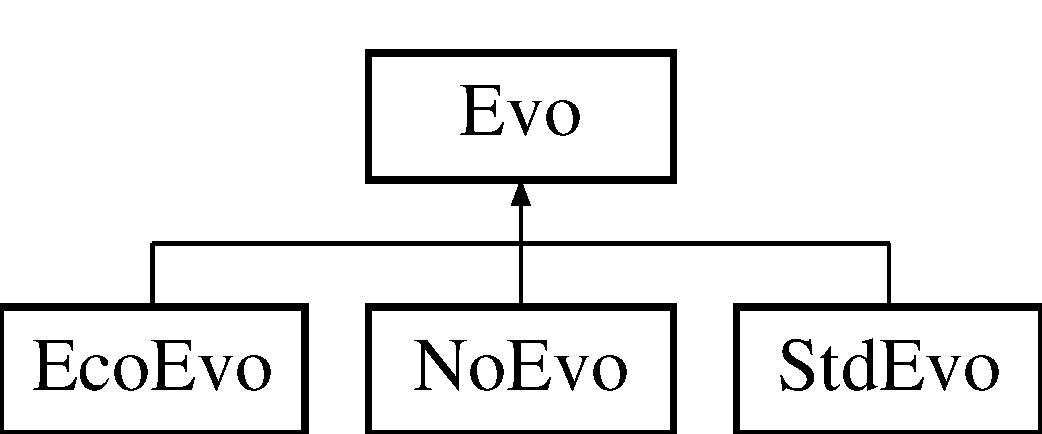
\includegraphics[height=2.000000cm]{classEvo}
\end{center}
\end{figure}
\subsection*{Public Member Functions}
\begin{DoxyCompactItemize}
\item 
\mbox{\Hypertarget{classEvo_adae2722f000f4838bae9743979b50328}\label{classEvo_adae2722f000f4838bae9743979b50328}} 
void {\bfseries set\+Delta} (double new\+Val)
\item 
virtual void \hyperlink{classEvo_a8c5208c00d1ee2fe9bef41bdd7fe0ab7}{get\+Evo} (vector$<$ unique\+\_\+ptr$<$ \hyperlink{classSpecies}{Species} $>$$>$ $\ast$species\+List, \hyperlink{classSpecies}{Species} $\ast$spec, int resolution)=0
\begin{DoxyCompactList}\small\item\em Controller method for updating species interactions/optimum. \end{DoxyCompactList}\item 
virtual vector$<$ unique\+\_\+ptr$<$ \hyperlink{classIndividual}{Individual} $>$ $>$ \hyperlink{classEvo_a88b5e0b1053cf1b4b473a08e2f03db92}{get\+Inds} (vector$<$ unique\+\_\+ptr$<$ \hyperlink{classSpecies}{Species} $>$$>$ $\ast$species\+List, \hyperlink{classSpecies}{Species} $\ast$spec, int resolution)=0
\begin{DoxyCompactList}\small\item\em Method for creating individuals from species. \end{DoxyCompactList}\item 
virtual vector$<$ int $>$ \hyperlink{classEvo_a10ff4eefe3967ff5cf5f820890c18079}{run\+Selection} (vector$<$ unique\+\_\+ptr$<$ \hyperlink{classIndividual}{Individual} $>$$>$ $\ast$inds, vector$<$ unique\+\_\+ptr$<$ \hyperlink{classSpecies}{Species} $>$$>$ $\ast$species\+List)=0
\begin{DoxyCompactList}\small\item\em Method that selects surviving/reproducing individuals. \end{DoxyCompactList}\end{DoxyCompactItemize}
\subsection*{Protected Attributes}
\begin{DoxyCompactItemize}
\item 
double \hyperlink{classEvo_a8f02598dfb1249ad135fbc741c27e0e0}{delta}
\end{DoxyCompactItemize}


\subsection{Detailed Description}
Class containing three methods used to calculate evolutionary change in species (virtual). 

The \hyperlink{classEvo}{Evo} class has three methods that are used to calculate change in species attributes (interactions/optimum). \hyperlink{classEvo_a8c5208c00d1ee2fe9bef41bdd7fe0ab7}{get\+Evo()} is the controller method, \hyperlink{classEvo_a88b5e0b1053cf1b4b473a08e2f03db92}{get\+Inds()} divides the species into individuals, and \hyperlink{classEvo_a10ff4eefe3967ff5cf5f820890c18079}{run\+Selection()} selects surviving/reproducing individuals. 

\subsection{Member Function Documentation}
\mbox{\Hypertarget{classEvo_a8c5208c00d1ee2fe9bef41bdd7fe0ab7}\label{classEvo_a8c5208c00d1ee2fe9bef41bdd7fe0ab7}} 
\index{Evo@{Evo}!get\+Evo@{get\+Evo}}
\index{get\+Evo@{get\+Evo}!Evo@{Evo}}
\subsubsection{\texorpdfstring{get\+Evo()}{getEvo()}}
{\footnotesize\ttfamily virtual void Evo\+::get\+Evo (\begin{DoxyParamCaption}\item[{vector$<$ unique\+\_\+ptr$<$ \hyperlink{classSpecies}{Species} $>$$>$ $\ast$}]{species\+List,  }\item[{\hyperlink{classSpecies}{Species} $\ast$}]{spec,  }\item[{int}]{resolution }\end{DoxyParamCaption})\hspace{0.3cm}{\ttfamily [pure virtual]}}



Controller method for updating species interactions/optimum. 

This method controls the evolutionary process, dividing the species into the right amount of individuals, selecting among them, and updating species interactions and optimum accordingly (for a more detailed description, see implementations).


\begin{DoxyParams}{Parameters}
{\em species\+List} & List containing all (alive) species present in the environment (used to calculate survival/reproduction probability of indivduals). \\
\hline
{\em spec} & \hyperlink{classSpecies}{Species} for which we will calculate evolutionary change (parameters are automatically updated during call). \\
\hline
{\em resolution} & How many discrete individuals are contained in one unit of density. \\
\hline
\end{DoxyParams}


Implemented in \hyperlink{classEcoEvo_a93564a6d93cdc1802182273c353e0552}{Eco\+Evo}, \hyperlink{classStdEvo_aa2b036f5e38510eca6cdbd60fc2bb23f}{Std\+Evo}, and \hyperlink{classNoEvo_ad43cc958ff310c4767725c5f4a7e7ac4}{No\+Evo}.

\mbox{\Hypertarget{classEvo_a88b5e0b1053cf1b4b473a08e2f03db92}\label{classEvo_a88b5e0b1053cf1b4b473a08e2f03db92}} 
\index{Evo@{Evo}!get\+Inds@{get\+Inds}}
\index{get\+Inds@{get\+Inds}!Evo@{Evo}}
\subsubsection{\texorpdfstring{get\+Inds()}{getInds()}}
{\footnotesize\ttfamily virtual vector$<$unique\+\_\+ptr$<$\hyperlink{classIndividual}{Individual}$>$ $>$ Evo\+::get\+Inds (\begin{DoxyParamCaption}\item[{vector$<$ unique\+\_\+ptr$<$ \hyperlink{classSpecies}{Species} $>$$>$ $\ast$}]{species\+List,  }\item[{\hyperlink{classSpecies}{Species} $\ast$}]{spec,  }\item[{int}]{resolution }\end{DoxyParamCaption})\hspace{0.3cm}{\ttfamily [pure virtual]}}



Method for creating individuals from species. 

This method divides a species with continous density into a discrete number of individuals {\ttfamily num\+Inds = round(species.\+density) $\ast$ resolution + 1$<$$>$ (+1 to avoid divide-\/by-\/zero errors. For a more detailed description, see implementations).}

{\ttfamily 
\begin{DoxyParams}{Parameters}
{\em species\+List} & List containing all (alive) species present in the environment (used to calculate survival/reproduction probability of indivduals). \\
\hline
{\em spec} & \hyperlink{classSpecies}{Species} from which we will generate individuals. \\
\hline
{\em resolution} & How many discrete individuals are contained in one unit of density. \\
\hline
\end{DoxyParams}
}

Implemented in \hyperlink{classEcoEvo_a819363c533784efea949ebc70a6d4636}{Eco\+Evo}, \hyperlink{classStdEvo_a40bd3beb0e6f36baee1b40db279fd9b4}{Std\+Evo}, and \hyperlink{classNoEvo_a9545e4f14c2038b8b7cab9362cb5fa9a}{No\+Evo}.

\mbox{\Hypertarget{classEvo_a10ff4eefe3967ff5cf5f820890c18079}\label{classEvo_a10ff4eefe3967ff5cf5f820890c18079}} 
\index{Evo@{Evo}!run\+Selection@{run\+Selection}}
\index{run\+Selection@{run\+Selection}!Evo@{Evo}}
\subsubsection{\texorpdfstring{run\+Selection()}{runSelection()}}
{\footnotesize\ttfamily virtual vector$<$int$>$ Evo\+::run\+Selection (\begin{DoxyParamCaption}\item[{vector$<$ unique\+\_\+ptr$<$ \hyperlink{classIndividual}{Individual} $>$$>$ $\ast$}]{inds,  }\item[{vector$<$ unique\+\_\+ptr$<$ \hyperlink{classSpecies}{Species} $>$$>$ $\ast$}]{species\+List }\end{DoxyParamCaption})\hspace{0.3cm}{\ttfamily [pure virtual]}}



Method that selects surviving/reproducing individuals. 

This method calculates survival/reproduction probability for each individual, and puts the number of existing copies of them in the vector it returns (for a more detailed description, see implementations).


\begin{DoxyParams}{Parameters}
{\em inds} & List containing all individuals that were generated from evolving species. \\
\hline
{\em species\+List} & List containing all (alive) species present in the environment (used to calculate survival/reproduction probability of indivduals). \\
\hline
\end{DoxyParams}


Implemented in \hyperlink{classEcoEvo_adfd00eb377489649a279e567abc3ae94}{Eco\+Evo}, \hyperlink{classStdEvo_a6d4c64918a01dd00ad5185796b67e219}{Std\+Evo}, and \hyperlink{classNoEvo_ae404207f48accfa7ea9f0022ed1af187}{No\+Evo}.



\subsection{Field Documentation}
\mbox{\Hypertarget{classEvo_a8f02598dfb1249ad135fbc741c27e0e0}\label{classEvo_a8f02598dfb1249ad135fbc741c27e0e0}} 
\index{Evo@{Evo}!delta@{delta}}
\index{delta@{delta}!Evo@{Evo}}
\subsubsection{\texorpdfstring{delta}{delta}}
{\footnotesize\ttfamily double Evo\+::delta\hspace{0.3cm}{\ttfamily [protected]}}

Delta used to calculate survival probability (same value as simulation delta) 

The documentation for this class was generated from the following file\+:\begin{DoxyCompactItemize}
\item 
\hyperlink{Evo_8hpp}{Evo.\+hpp}\end{DoxyCompactItemize}

\hypertarget{classEvoMultiNextGen}{}\section{Evo\+Multi\+Next\+Gen Class Reference}
\label{classEvoMultiNextGen}\index{Evo\+Multi\+Next\+Gen@{Evo\+Multi\+Next\+Gen}}


Class containing a single method, used to control transition from one step to the next, and update Species/\+Environemnt attributes.  




{\ttfamily \#include $<$Evo\+Multi\+Next\+Gen.\+hpp$>$}

Inheritance diagram for Evo\+Multi\+Next\+Gen\+:\begin{figure}[H]
\begin{center}
\leavevmode
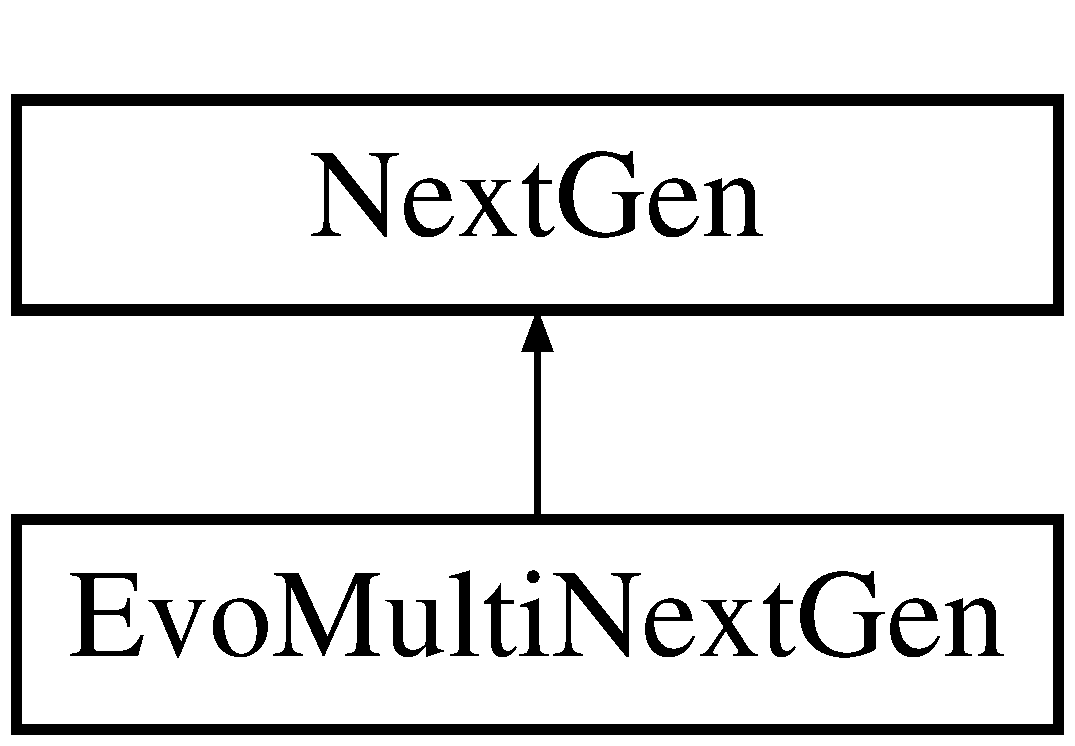
\includegraphics[height=2.000000cm]{classEvoMultiNextGen}
\end{center}
\end{figure}
\subsection*{Public Member Functions}
\begin{DoxyCompactItemize}
\item 
void \hyperlink{classEvoMultiNextGen_acab6fd876dc02feae353b52461b88861}{get\+Next\+Gen} (int step\+Num, std\+::vector$<$ std\+::unique\+\_\+ptr$<$ \hyperlink{classSpecies}{Species} $>$$>$ $\ast$species\+List, \hyperlink{classEnvironment}{Environment} $\ast$env)
\begin{DoxyCompactList}\small\item\em Method used to update \hyperlink{classSpecies}{Species} density at each timestep. \end{DoxyCompactList}\end{DoxyCompactItemize}


\subsection{Detailed Description}
Class containing a single method, used to control transition from one step to the next, and update Species/\+Environemnt attributes. 

\subsection{Member Function Documentation}
\hypertarget{classEvoMultiNextGen_acab6fd876dc02feae353b52461b88861}{}\label{classEvoMultiNextGen_acab6fd876dc02feae353b52461b88861} 
\index{Evo\+Multi\+Next\+Gen@{Evo\+Multi\+Next\+Gen}!get\+Next\+Gen@{get\+Next\+Gen}}
\index{get\+Next\+Gen@{get\+Next\+Gen}!Evo\+Multi\+Next\+Gen@{Evo\+Multi\+Next\+Gen}}
\subsubsection{\texorpdfstring{get\+Next\+Gen()}{getNextGen()}}
{\footnotesize\ttfamily void Evo\+Multi\+Next\+Gen\+::get\+Next\+Gen (\begin{DoxyParamCaption}\item[{int}]{step\+Num,  }\item[{std\+::vector$<$ std\+::unique\+\_\+ptr$<$ \hyperlink{classSpecies}{Species} $>$$>$ $\ast$}]{species\+List,  }\item[{\hyperlink{classEnvironment}{Environment} $\ast$}]{env }\end{DoxyParamCaption})\hspace{0.3cm}{\ttfamily [virtual]}}



Method used to update \hyperlink{classSpecies}{Species} density at each timestep. 

This method works exactly like the one in \hyperlink{classEvoNextGen}{Evo\+Next\+Gen}, except that species with {\ttfamily density == 0} are not moved to env.\+dead\+Species, to avoid having to recreate them if a population from said species migrates into environment from somewhere. If migration probability is very low for all species, it might be worth to delete/introduce them each time, since this might take less time than the increased loop time caused by a higher number of species (I\textquotesingle{}d say it depends on the simulation parameters, but I haven\textquotesingle{}t done any performance tests to compare the two methods).


\begin{DoxyParams}{Parameters}
{\em step\+Num} & Values of the current step \\
\hline
{\em species\+List} & List containing all \hyperlink{classSpecies}{Species} of the environment \\
\hline
{\em env} & Pointer to current environment \\
\hline
\end{DoxyParams}


Implements \hyperlink{classNextGen_aa70da77e0ac03da1bd5414c5e3fd70c0}{Next\+Gen}.



The documentation for this class was generated from the following files\+:\begin{DoxyCompactItemize}
\item 
\hyperlink{EvoMultiNextGen_8hpp}{Evo\+Multi\+Next\+Gen.\+hpp}\item 
Evo\+Multi\+Next\+Gen.\+cpp\end{DoxyCompactItemize}

\hypertarget{classEvoNextGen}{}\section{Evo\+Next\+Gen Class Reference}
\label{classEvoNextGen}\index{Evo\+Next\+Gen@{Evo\+Next\+Gen}}


Class containing a single method, used to control transition from one step to the next, and update Species/\+Environemnt attributes.  




{\ttfamily \#include $<$Evo\+Next\+Gen.\+hpp$>$}

Inheritance diagram for Evo\+Next\+Gen\+:\begin{figure}[H]
\begin{center}
\leavevmode
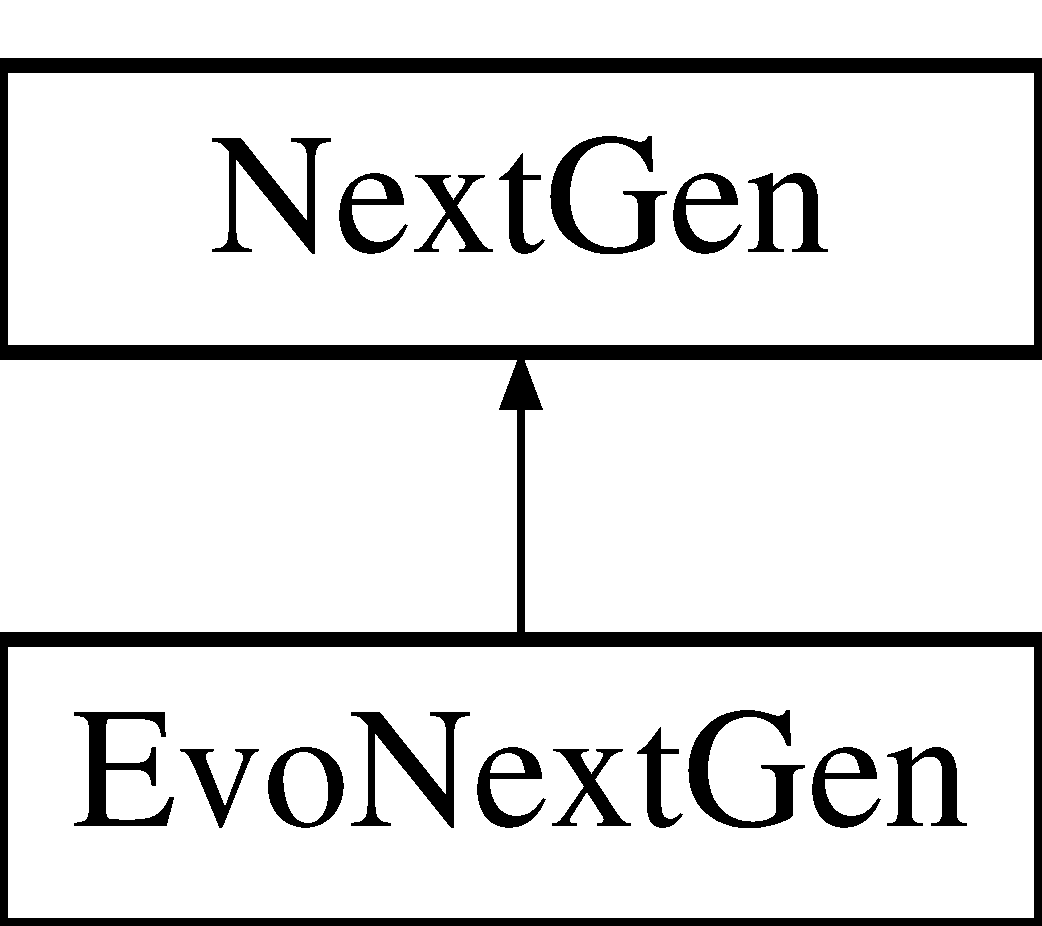
\includegraphics[height=2.000000cm]{classEvoNextGen}
\end{center}
\end{figure}
\subsection*{Public Member Functions}
\begin{DoxyCompactItemize}
\item 
void \hyperlink{classEvoNextGen_af9ee37c63b6b2c22d27194b6b507c75a}{get\+Next\+Gen} (int step\+Num, std\+::vector$<$ std\+::unique\+\_\+ptr$<$ \hyperlink{classSpecies}{Species} $>$$>$ $\ast$species\+List, \hyperlink{classEnvironment}{Environment} $\ast$env)
\begin{DoxyCompactList}\small\item\em Method used to update \hyperlink{classSpecies}{Species} density and interactions at each timestep. \end{DoxyCompactList}\end{DoxyCompactItemize}


\subsection{Detailed Description}
Class containing a single method, used to control transition from one step to the next, and update Species/\+Environemnt attributes. 

\subsection{Member Function Documentation}
\hypertarget{classEvoNextGen_af9ee37c63b6b2c22d27194b6b507c75a}{}\label{classEvoNextGen_af9ee37c63b6b2c22d27194b6b507c75a} 
\index{Evo\+Next\+Gen@{Evo\+Next\+Gen}!get\+Next\+Gen@{get\+Next\+Gen}}
\index{get\+Next\+Gen@{get\+Next\+Gen}!Evo\+Next\+Gen@{Evo\+Next\+Gen}}
\subsubsection{\texorpdfstring{get\+Next\+Gen()}{getNextGen()}}
{\footnotesize\ttfamily void Evo\+Next\+Gen\+::get\+Next\+Gen (\begin{DoxyParamCaption}\item[{int}]{step\+Num,  }\item[{std\+::vector$<$ std\+::unique\+\_\+ptr$<$ \hyperlink{classSpecies}{Species} $>$$>$ $\ast$}]{species\+List,  }\item[{\hyperlink{classEnvironment}{Environment} $\ast$}]{env }\end{DoxyParamCaption})\hspace{0.3cm}{\ttfamily [virtual]}}



Method used to update \hyperlink{classSpecies}{Species} density and interactions at each timestep. 

This method works much in the same way as that of \hyperlink{classStdNextGen}{Std\+Next\+Gen}, except that after calculating cahnge in \hyperlink{classSpecies}{Species} density for all species (and moving dead species), it calls spec.\+get\+Evo() on each \hyperlink{classSpecies}{Species} where {\ttfamily step\+Numspec.\+evo\+Rate == 0}


\begin{DoxyParams}{Parameters}
{\em step\+Num} & Values of the current step \\
\hline
{\em species\+List} & List containing all \hyperlink{classSpecies}{Species} of the environment \\
\hline
{\em env} & Pointer to current environment \\
\hline
\end{DoxyParams}


Implements \hyperlink{classNextGen_aa70da77e0ac03da1bd5414c5e3fd70c0}{Next\+Gen}.



The documentation for this class was generated from the following files\+:\begin{DoxyCompactItemize}
\item 
\hyperlink{EvoNextGen_8hpp}{Evo\+Next\+Gen.\+hpp}\item 
Evo\+Next\+Gen.\+cpp\end{DoxyCompactItemize}

\hypertarget{classEvoSimulation}{}\section{Evo\+Simulation Class Reference}
\label{classEvoSimulation}\index{Evo\+Simulation@{Evo\+Simulation}}


Class containing all \hyperlink{classEnvironment}{Environment} objects, as well control-\/flow attributes for the simulation.  




{\ttfamily \#include $<$Evo\+Simulation.\+hpp$>$}

Inheritance diagram for Evo\+Simulation\+:\begin{figure}[H]
\begin{center}
\leavevmode
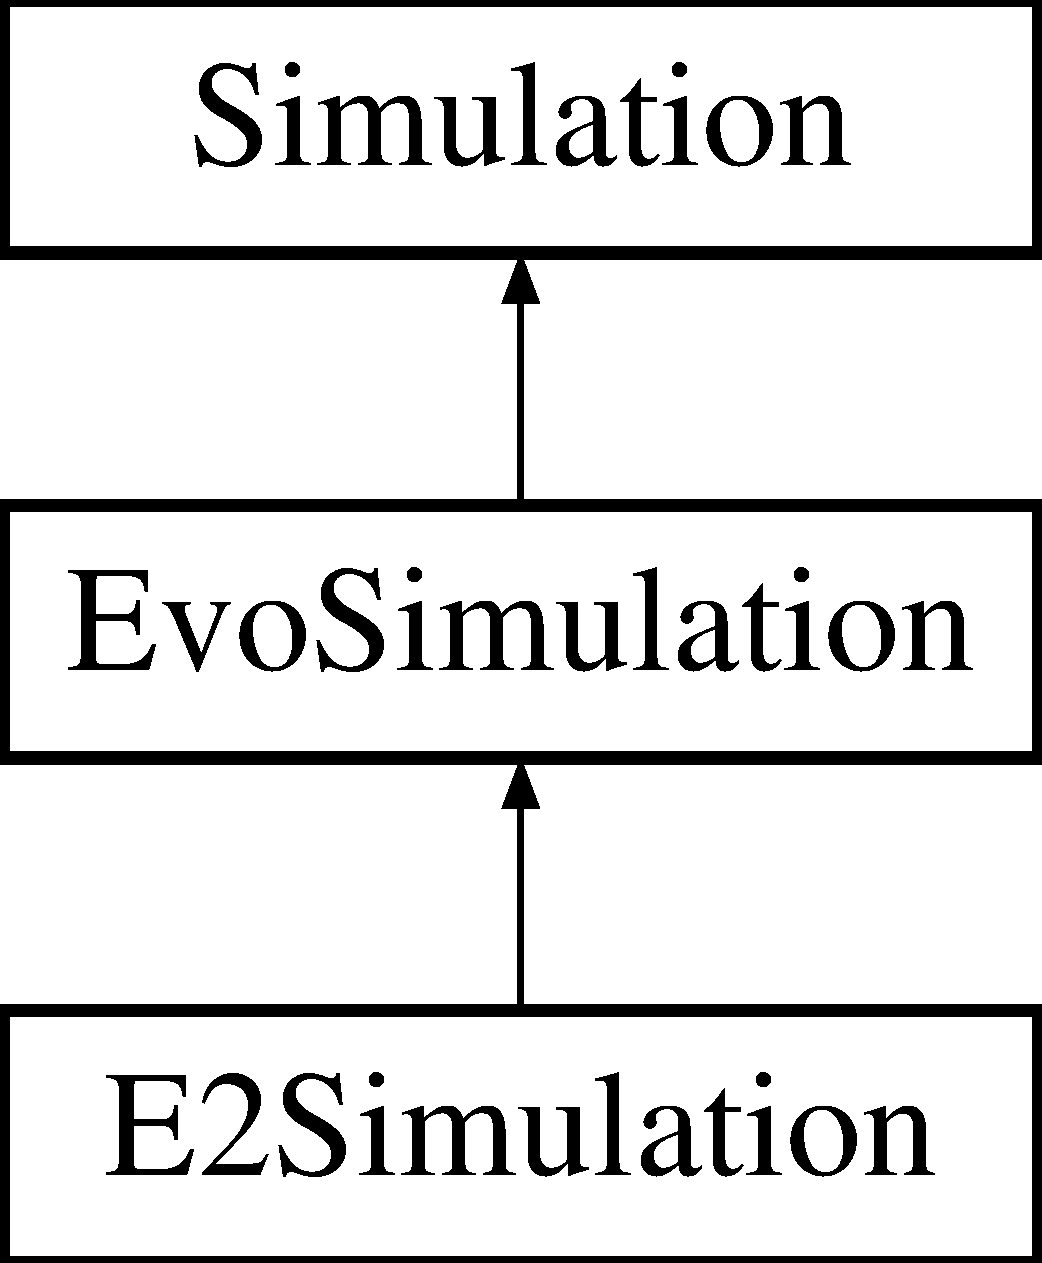
\includegraphics[height=3.000000cm]{classEvoSimulation}
\end{center}
\end{figure}
\subsection*{Public Member Functions}
\begin{DoxyCompactItemize}
\item 
\mbox{\Hypertarget{classEvoSimulation_ad9c067c5d931cef3485671c652340fed}\label{classEvoSimulation_ad9c067c5d931cef3485671c652340fed}} 
{\bfseries Evo\+Simulation} (vector$<$ \hyperlink{classEnvironment}{Environment} $>$ \+\_\+env)
\item 
\mbox{\Hypertarget{classEvoSimulation_ad355ec692640389831d0f70ee5336371}\label{classEvoSimulation_ad355ec692640389831d0f70ee5336371}} 
int {\bfseries get\+Inter\+Save\+Div} ()
\item 
\mbox{\Hypertarget{classEvoSimulation_afcd50bb904037e0ed92f82db5bce4706}\label{classEvoSimulation_afcd50bb904037e0ed92f82db5bce4706}} 
void {\bfseries set\+Inter\+Save\+Div} (int new\+Val)
\item 
\mbox{\Hypertarget{classEvoSimulation_abc143157a5ee313cd04375e0b11fd25d}\label{classEvoSimulation_abc143157a5ee313cd04375e0b11fd25d}} 
vector$<$ \hyperlink{classEnvironment}{Environment} $>$ $\ast$ {\bfseries get\+Envs} ()
\item 
\mbox{\Hypertarget{classEvoSimulation_ae2c4e68c8181696f5c524c9f09f29421}\label{classEvoSimulation_ae2c4e68c8181696f5c524c9f09f29421}} 
void {\bfseries add\+Env} (\hyperlink{classEnvironment}{Environment} new\+Val)
\item 
\mbox{\Hypertarget{classEvoSimulation_ae075e1877fb4c1132f4630a85ed5fcbf}\label{classEvoSimulation_ae075e1877fb4c1132f4630a85ed5fcbf}} 
void {\bfseries set\+Env} (\hyperlink{classEnvironment}{Environment} new\+Val)
\item 
virtual int \hyperlink{classEvoSimulation_aa43aa351dec24c638e56995a67a4f0f5}{run\+Sim} (int run\+Number)
\begin{DoxyCompactList}\small\item\em Method that runs the main loop of the simulation. \end{DoxyCompactList}\end{DoxyCompactItemize}
\subsection*{Protected Attributes}
\begin{DoxyCompactItemize}
\item 
\mbox{\Hypertarget{classEvoSimulation_ac75fd2b2c9fb588adb138c0c0aaebe4d}\label{classEvoSimulation_ac75fd2b2c9fb588adb138c0c0aaebe4d}} 
vector$<$ \hyperlink{classEnvironment}{Environment} $>$ {\bfseries envs}
\item 
int \hyperlink{classEvoSimulation_aced0330991a4c4ed3bf726e5909fbd31}{inter\+Save\+Div}
\end{DoxyCompactItemize}


\subsection{Detailed Description}
Class containing all \hyperlink{classEnvironment}{Environment} objects, as well control-\/flow attributes for the simulation. 

The Evo\+Simulaiton class is very similar to the simulation class, except that it can also save interaction values of species during simulaiton execution (to track changes due to evolution). 

\subsection{Member Function Documentation}
\mbox{\Hypertarget{classEvoSimulation_aa43aa351dec24c638e56995a67a4f0f5}\label{classEvoSimulation_aa43aa351dec24c638e56995a67a4f0f5}} 
\index{Evo\+Simulation@{Evo\+Simulation}!run\+Sim@{run\+Sim}}
\index{run\+Sim@{run\+Sim}!Evo\+Simulation@{Evo\+Simulation}}
\subsubsection{\texorpdfstring{run\+Sim()}{runSim()}}
{\footnotesize\ttfamily int Evo\+Simulation\+::run\+Sim (\begin{DoxyParamCaption}\item[{int}]{run\+Number }\end{DoxyParamCaption})\hspace{0.3cm}{\ttfamily [virtual]}}



Method that runs the main loop of the simulation. 


\begin{DoxyParams}{Parameters}
{\em run\+Number} & ID of the current run of the simulation. \\
\hline
\end{DoxyParams}


Reimplemented from \hyperlink{classSimulation_a7eb16da89581b496d33b77efbb63b9cd}{Simulation}.



Reimplemented in \hyperlink{classE2Simulation_a28028881fd443d2445b562512cb2169c}{E2\+Simulation}.



\subsection{Field Documentation}
\mbox{\Hypertarget{classEvoSimulation_aced0330991a4c4ed3bf726e5909fbd31}\label{classEvoSimulation_aced0330991a4c4ed3bf726e5909fbd31}} 
\index{Evo\+Simulation@{Evo\+Simulation}!inter\+Save\+Div@{inter\+Save\+Div}}
\index{inter\+Save\+Div@{inter\+Save\+Div}!Evo\+Simulation@{Evo\+Simulation}}
\subsubsection{\texorpdfstring{inter\+Save\+Div}{interSaveDiv}}
{\footnotesize\ttfamily int Evo\+Simulation\+::inter\+Save\+Div\hspace{0.3cm}{\ttfamily [protected]}}

Each how many timesteps interaction values are saved for species (in raw\+Save file) 

The documentation for this class was generated from the following files\+:\begin{DoxyCompactItemize}
\item 
\hyperlink{EvoSimulation_8hpp}{Evo\+Simulation.\+hpp}\item 
Evo\+Simulation.\+cpp\end{DoxyCompactItemize}

\hypertarget{classI2}{}\section{I2 Class Reference}
\label{classI2}\index{I2@{I2}}


Class used to discretize continous species density, so as to select from during evolution events.  




{\ttfamily \#include $<$I2.\+hpp$>$}

Inheritance diagram for I2\+:\begin{figure}[H]
\begin{center}
\leavevmode
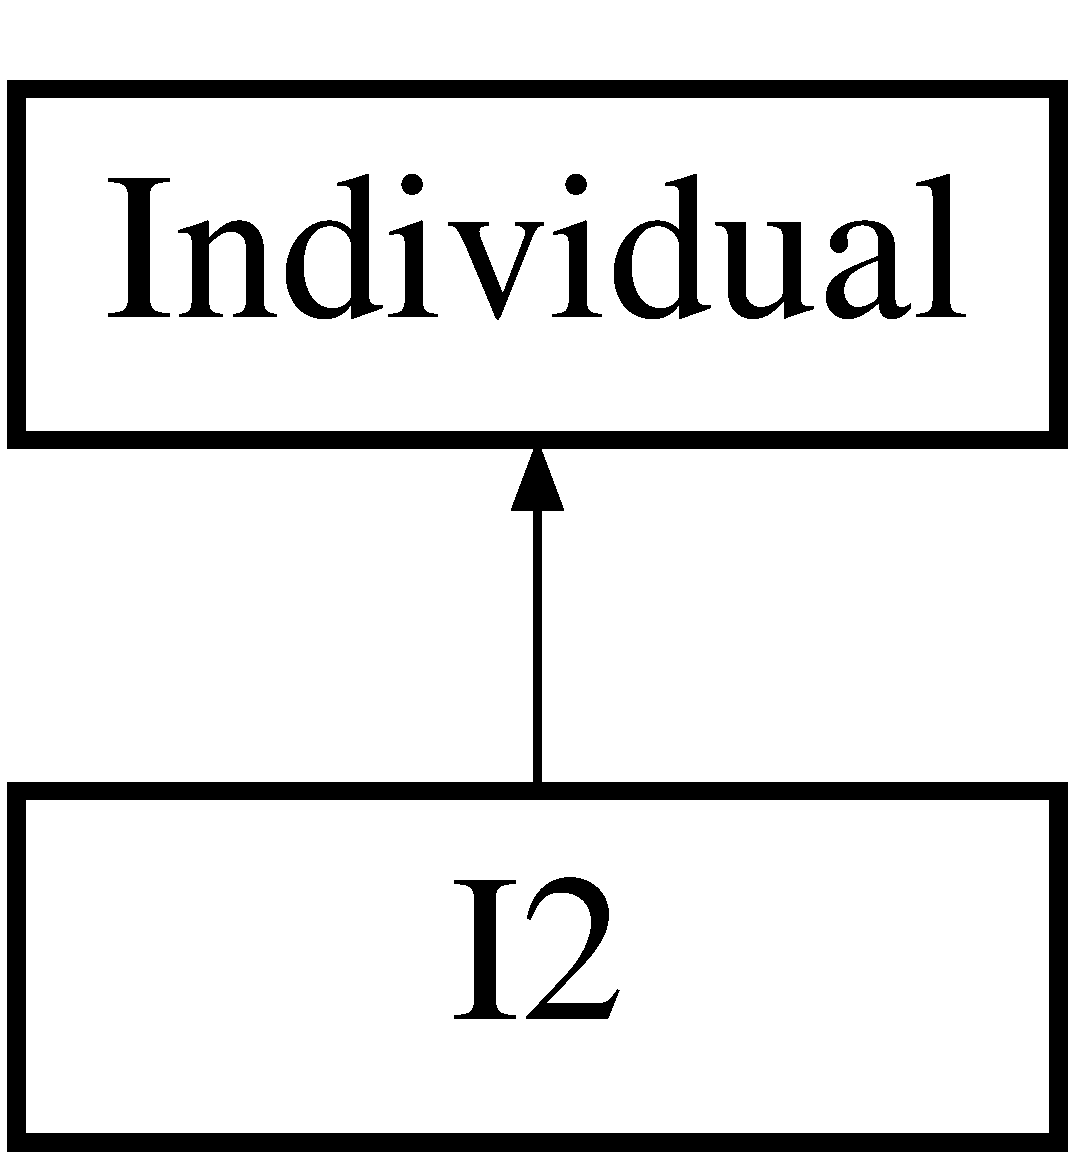
\includegraphics[height=2.000000cm]{classI2}
\end{center}
\end{figure}
\subsection*{Public Member Functions}
\begin{DoxyCompactItemize}
\item 
\hypertarget{classI2_a6b6f833683560c884852c507d489d99e}{}\label{classI2_a6b6f833683560c884852c507d489d99e} 
{\bfseries I2} (double $\ast$const \+\_\+env\+Const)
\item 
double \hyperlink{classI2_ac747249e352a954b96a530537c60d3b1}{get\+Survival} (vector$<$ unique\+\_\+ptr$<$ \hyperlink{classSpecies}{Species} $>$$>$ $\ast$all\+Specs, double delta)
\begin{DoxyCompactList}\small\item\em Method to calculate survival/reproduction probability of individual. \end{DoxyCompactList}\end{DoxyCompactItemize}
\subsection*{Public Attributes}
\begin{DoxyCompactItemize}
\item 
double $\ast$const \hyperlink{classI2_a16f94b60e5a6c02c67a46500798fd7cf}{env\+Const}
\item 
double \hyperlink{classI2_a5f022bb4d32b5ee96e117b72e17b262a}{optimum}
\end{DoxyCompactItemize}


\subsection{Detailed Description}
Class used to discretize continous species density, so as to select from during evolution events. 

The \hyperlink{classI2}{I2} class is used much like its parent class, but \hyperlink{classI2_ac747249e352a954b96a530537c60d3b1}{get\+Survival()} takes the environmental constant into account when calculating survival/reproduction probability. 

\subsection{Member Function Documentation}
\hypertarget{classI2_ac747249e352a954b96a530537c60d3b1}{}\label{classI2_ac747249e352a954b96a530537c60d3b1} 
\index{I2@{I2}!get\+Survival@{get\+Survival}}
\index{get\+Survival@{get\+Survival}!I2@{I2}}
\subsubsection{\texorpdfstring{get\+Survival()}{getSurvival()}}
{\footnotesize\ttfamily double I2\+::get\+Survival (\begin{DoxyParamCaption}\item[{vector$<$ unique\+\_\+ptr$<$ \hyperlink{classSpecies}{Species} $>$$>$ $\ast$}]{all\+Specs,  }\item[{double}]{delta }\end{DoxyParamCaption})\hspace{0.3cm}{\ttfamily [virtual]}}



Method to calculate survival/reproduction probability of individual. 

Much the same as in \hyperlink{classIndividual}{Individual}, except that, if survival/reproduction probability is higher than 0.\+5, then\+:

$survivalProb = 0.5 + (survivalProb - 0.5)*e^{-(optimum-(*envConst))^2}$


\begin{DoxyParams}{Parameters}
{\em species\+List} & List containing all (alive) species in the environment \\
\hline
{\em delta} & Size of timestep of simulation \\
\hline
\end{DoxyParams}


Reimplemented from \hyperlink{classIndividual_a895954f2c3a683dd3bd7475651a38160}{Individual}.



\subsection{Member Data Documentation}
\hypertarget{classI2_a16f94b60e5a6c02c67a46500798fd7cf}{}\label{classI2_a16f94b60e5a6c02c67a46500798fd7cf} 
\index{I2@{I2}!env\+Const@{env\+Const}}
\index{env\+Const@{env\+Const}!I2@{I2}}
\subsubsection{\texorpdfstring{env\+Const}{envConst}}
{\footnotesize\ttfamily double$\ast$ const I2\+::env\+Const}

Pointer to the environmental constant (owned by \hyperlink{classEnvironment}{Environment}) \hypertarget{classI2_a5f022bb4d32b5ee96e117b72e17b262a}{}\label{classI2_a5f022bb4d32b5ee96e117b72e17b262a} 
\index{I2@{I2}!optimum@{optimum}}
\index{optimum@{optimum}!I2@{I2}}
\subsubsection{\texorpdfstring{optimum}{optimum}}
{\footnotesize\ttfamily double I2\+::optimum}

\hyperlink{classIndividual}{Individual} optimum (value for env\+Const at which it thrives best) 

The documentation for this class was generated from the following files\+:\begin{DoxyCompactItemize}
\item 
\hyperlink{I2_8hpp}{I2.\+hpp}\item 
I2.\+cpp\end{DoxyCompactItemize}

\hypertarget{classIndividual}{}\section{Individual Class Reference}
\label{classIndividual}\index{Individual@{Individual}}


Class used to discretize continous species density, so as to select from during evolution events.  




{\ttfamily \#include $<$Individual.\+hpp$>$}

Inheritance diagram for Individual\+:\begin{figure}[H]
\begin{center}
\leavevmode
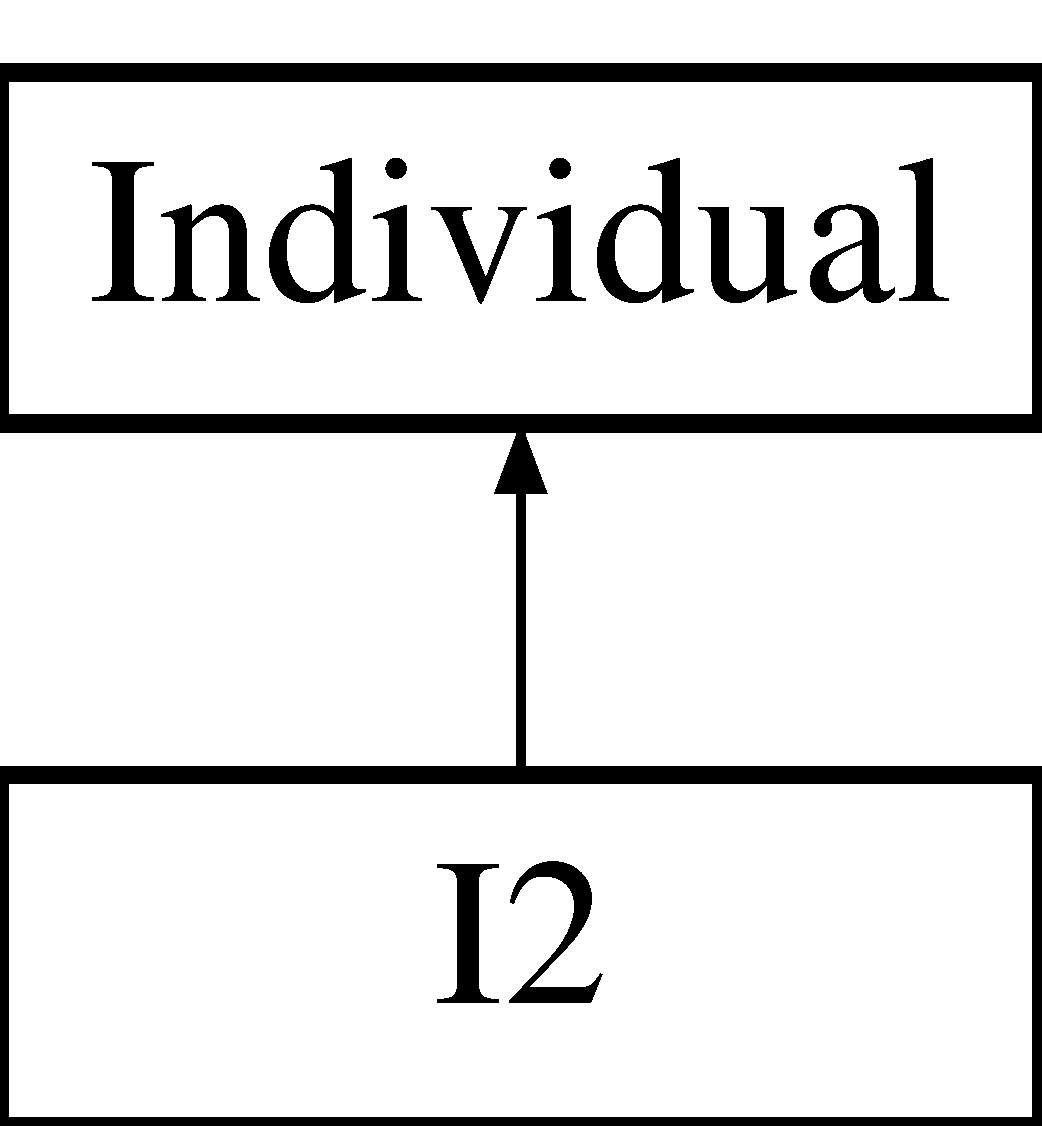
\includegraphics[height=2.000000cm]{classIndividual}
\end{center}
\end{figure}
\subsection*{Public Member Functions}
\begin{DoxyCompactItemize}
\item 
virtual double \hyperlink{classIndividual_a895954f2c3a683dd3bd7475651a38160}{get\+Survival} (vector$<$ unique\+\_\+ptr$<$ \hyperlink{classSpecies}{Species} $>$$>$ $\ast$all\+Specs, double delta)
\begin{DoxyCompactList}\small\item\em Method to calculate survival/reproduction probability of individual. \end{DoxyCompactList}\end{DoxyCompactItemize}
\subsection*{Data Fields}
\begin{DoxyCompactItemize}
\item 
int \hyperlink{classIndividual_a2a7068df27211ad0b2e869a3c628cd9f}{spec\+ID}
\item 
double \hyperlink{classIndividual_adc6dbb93690c48fbba745ce0fcf6d5b0}{optimum}
\item 
int \hyperlink{classIndividual_a78e6327a339aa73f73d81e991b3fede2}{num\+Total}
\item 
vector$<$ double $>$ \hyperlink{classIndividual_ac832077568d1e59f979af3fe6bd7e3e6}{interactions}
\item 
double \hyperlink{classIndividual_adbd7cefa7cf5847a6a20e14c04ab20dd}{survival} = 0
\end{DoxyCompactItemize}


\subsection{Detailed Description}
Class used to discretize continous species density, so as to select from during evolution events. 

The \hyperlink{classIndividual}{Individual} class is used to represent discrete individuals of a species (which has continous density). It has a similar (but much more restricted) set of attributes as \hyperlink{classSpecies}{Species}, although what is calculated by individuals is a probability of survival/reproduction, as opposed to a change in density (\hyperlink{classSpecies}{Species}). This class (and its inheritor) are used during evolution events to discretize species density (see \hyperlink{classEvo}{Evo} class). 

\subsection{Member Function Documentation}
\mbox{\Hypertarget{classIndividual_a895954f2c3a683dd3bd7475651a38160}\label{classIndividual_a895954f2c3a683dd3bd7475651a38160}} 
\index{Individual@{Individual}!get\+Survival@{get\+Survival}}
\index{get\+Survival@{get\+Survival}!Individual@{Individual}}
\subsubsection{\texorpdfstring{get\+Survival()}{getSurvival()}}
{\footnotesize\ttfamily double Individual\+::get\+Survival (\begin{DoxyParamCaption}\item[{vector$<$ unique\+\_\+ptr$<$ \hyperlink{classSpecies}{Species} $>$$>$ $\ast$}]{all\+Specs,  }\item[{double}]{delta }\end{DoxyParamCaption})\hspace{0.3cm}{\ttfamily [virtual]}}



Method to calculate survival/reproduction probability of individual. 

This method calculates survival/reproduction porbability of the individual with equations similar to those used by the species\+:

$P(S_i) = \delta \cdot \sum_{j \neg i} II_{ij}*x_j +0.5$

where $II_{ij}$ is the interaction of individual i with species j, and $x_j$ is density of species j.


\begin{DoxyParams}{Parameters}
{\em species\+List} & List containing all (alive) species in the environment \\
\hline
{\em delta} & Size of time\+Step. \\
\hline
\end{DoxyParams}


Reimplemented in \hyperlink{classI2_ac747249e352a954b96a530537c60d3b1}{I2}.



\subsection{Field Documentation}
\mbox{\Hypertarget{classIndividual_ac832077568d1e59f979af3fe6bd7e3e6}\label{classIndividual_ac832077568d1e59f979af3fe6bd7e3e6}} 
\index{Individual@{Individual}!interactions@{interactions}}
\index{interactions@{interactions}!Individual@{Individual}}
\subsubsection{\texorpdfstring{interactions}{interactions}}
{\footnotesize\ttfamily vector$<$double$>$ Individual\+::interactions}

interaction values for individuals \mbox{\Hypertarget{classIndividual_a78e6327a339aa73f73d81e991b3fede2}\label{classIndividual_a78e6327a339aa73f73d81e991b3fede2}} 
\index{Individual@{Individual}!num\+Total@{num\+Total}}
\index{num\+Total@{num\+Total}!Individual@{Individual}}
\subsubsection{\texorpdfstring{num\+Total}{numTotal}}
{\footnotesize\ttfamily int Individual\+::num\+Total}

Total number of species at start of simulation \mbox{\Hypertarget{classIndividual_adc6dbb93690c48fbba745ce0fcf6d5b0}\label{classIndividual_adc6dbb93690c48fbba745ce0fcf6d5b0}} 
\index{Individual@{Individual}!optimum@{optimum}}
\index{optimum@{optimum}!Individual@{Individual}}
\subsubsection{\texorpdfstring{optimum}{optimum}}
{\footnotesize\ttfamily double Individual\+::optimum}

optimum of the individual (only used in simulations with evolution) \mbox{\Hypertarget{classIndividual_a2a7068df27211ad0b2e869a3c628cd9f}\label{classIndividual_a2a7068df27211ad0b2e869a3c628cd9f}} 
\index{Individual@{Individual}!spec\+ID@{spec\+ID}}
\index{spec\+ID@{spec\+ID}!Individual@{Individual}}
\subsubsection{\texorpdfstring{spec\+ID}{specID}}
{\footnotesize\ttfamily int Individual\+::spec\+ID}

ID of species the individual belongs to. \mbox{\Hypertarget{classIndividual_adbd7cefa7cf5847a6a20e14c04ab20dd}\label{classIndividual_adbd7cefa7cf5847a6a20e14c04ab20dd}} 
\index{Individual@{Individual}!survival@{survival}}
\index{survival@{survival}!Individual@{Individual}}
\subsubsection{\texorpdfstring{survival}{survival}}
{\footnotesize\ttfamily double Individual\+::survival = 0}

Probability that a given individual survives and reproduces 

The documentation for this class was generated from the following files\+:\begin{DoxyCompactItemize}
\item 
\hyperlink{Individual_8hpp}{Individual.\+hpp}\item 
Individual.\+cpp\end{DoxyCompactItemize}

\hypertarget{classMultiEcoSimulation}{}\section{Multi\+Eco\+Simulation Class Reference}
\label{classMultiEcoSimulation}\index{Multi\+Eco\+Simulation@{Multi\+Eco\+Simulation}}


Class containing all \hyperlink{classEnvironment}{Environment} objects, as well control-\/flow attributes for the simulation.  




{\ttfamily \#include $<$Multi\+Eco\+Simulation.\+hpp$>$}

Inheritance diagram for Multi\+Eco\+Simulation\+:\begin{figure}[H]
\begin{center}
\leavevmode
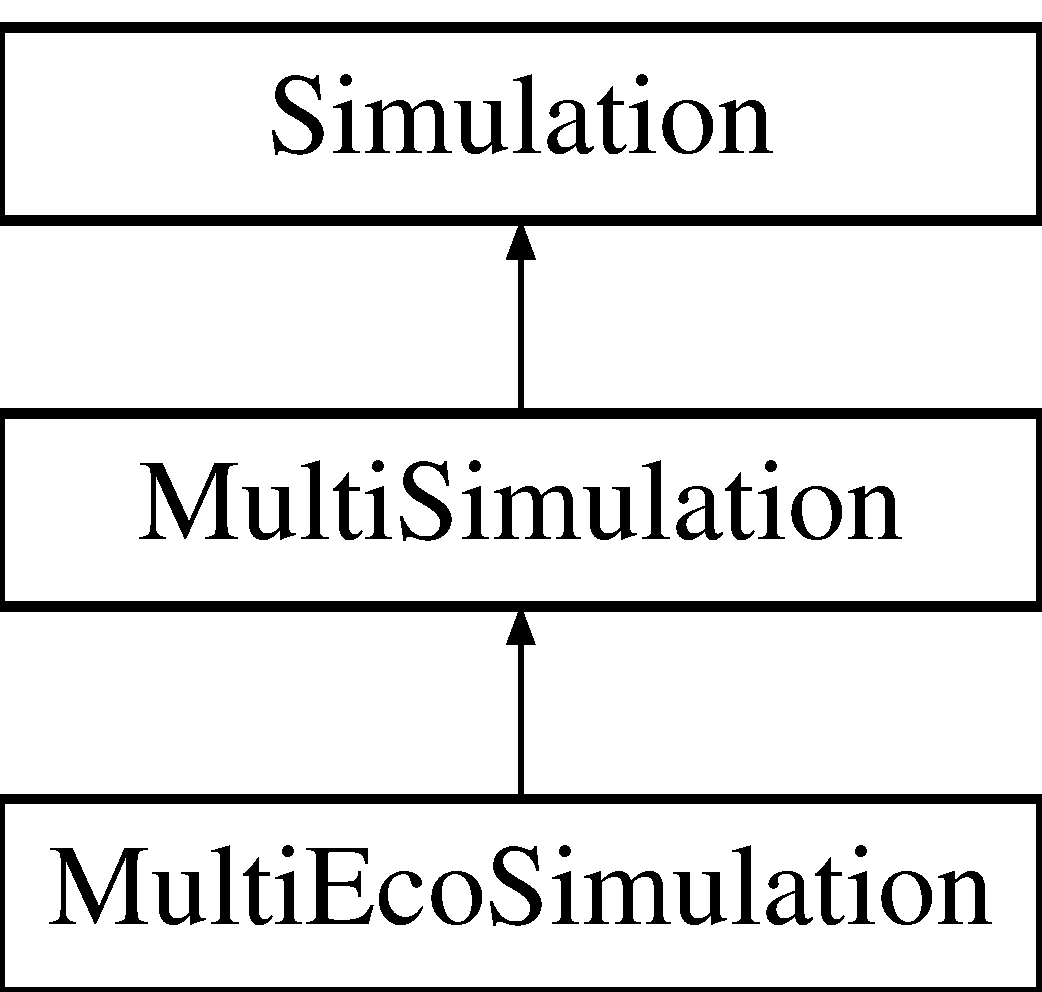
\includegraphics[height=3.000000cm]{classMultiEcoSimulation}
\end{center}
\end{figure}
\subsection*{Public Member Functions}
\begin{DoxyCompactItemize}
\item 
\mbox{\Hypertarget{classMultiEcoSimulation_af8a850bdfb77405c1e93b1f6549e36d8}\label{classMultiEcoSimulation_af8a850bdfb77405c1e93b1f6549e36d8}} 
{\bfseries Multi\+Eco\+Simulation} (vector$<$ \hyperlink{classEnvironment}{Environment} $>$ \+\_\+envs)
\item 
\mbox{\Hypertarget{classMultiEcoSimulation_a6bff1bcc1a05b2fdabfd3885ad62022f}\label{classMultiEcoSimulation_a6bff1bcc1a05b2fdabfd3885ad62022f}} 
vector$<$ \hyperlink{classEnvironment}{Environment} $>$ $\ast$ {\bfseries get\+Envs} ()
\item 
\mbox{\Hypertarget{classMultiEcoSimulation_a94ebc91936e91b516d4bd442b80a472e}\label{classMultiEcoSimulation_a94ebc91936e91b516d4bd442b80a472e}} 
void {\bfseries set\+Envs} (vector$<$ \hyperlink{classEnvironment}{Environment} $>$ new\+Val)
\item 
\mbox{\Hypertarget{classMultiEcoSimulation_ae8dd59a797f43d0fffd34ec3cdc06728}\label{classMultiEcoSimulation_ae8dd59a797f43d0fffd34ec3cdc06728}} 
void {\bfseries add\+Env} (\hyperlink{classEnvironment}{Environment} env)
\item 
int \hyperlink{classMultiEcoSimulation_ad490e089c083d06d80c62af9e1564ac3}{run\+Sim} (int run\+Number)
\begin{DoxyCompactList}\small\item\em Method that runs the main loop of the simulation. \end{DoxyCompactList}\end{DoxyCompactItemize}
\subsection*{Protected Attributes}
\begin{DoxyCompactItemize}
\item 
\mbox{\Hypertarget{classMultiEcoSimulation_ad3c5ac5fa8139145d797d0f47653838e}\label{classMultiEcoSimulation_ad3c5ac5fa8139145d797d0f47653838e}} 
vector$<$ \hyperlink{classEnvironment}{Environment} $>$ {\bfseries envs}
\end{DoxyCompactItemize}


\subsection{Detailed Description}
Class containing all \hyperlink{classEnvironment}{Environment} objects, as well control-\/flow attributes for the simulation. 

Same as \hyperlink{classEcoSimulation}{Eco\+Simulation}, but for simulations with multiple environments (see also \hyperlink{classMultiSimulation}{Multi\+Simulation}) 

\subsection{Member Function Documentation}
\mbox{\Hypertarget{classMultiEcoSimulation_ad490e089c083d06d80c62af9e1564ac3}\label{classMultiEcoSimulation_ad490e089c083d06d80c62af9e1564ac3}} 
\index{Multi\+Eco\+Simulation@{Multi\+Eco\+Simulation}!run\+Sim@{run\+Sim}}
\index{run\+Sim@{run\+Sim}!Multi\+Eco\+Simulation@{Multi\+Eco\+Simulation}}
\subsubsection{\texorpdfstring{run\+Sim()}{runSim()}}
{\footnotesize\ttfamily int Multi\+Eco\+Simulation\+::run\+Sim (\begin{DoxyParamCaption}\item[{int}]{run\+Number }\end{DoxyParamCaption})\hspace{0.3cm}{\ttfamily [virtual]}}



Method that runs the main loop of the simulation. 


\begin{DoxyParams}{Parameters}
{\em run\+Number} & ID of the current run of the simulation. \\
\hline
\end{DoxyParams}


Reimplemented from \hyperlink{classMultiSimulation_a235347d04fd0c7e1a2e35d7a39e77583}{Multi\+Simulation}.



The documentation for this class was generated from the following files\+:\begin{DoxyCompactItemize}
\item 
\hyperlink{MultiEcoSimulation_8hpp}{Multi\+Eco\+Simulation.\+hpp}\item 
Multi\+Eco\+Simulation.\+cpp\end{DoxyCompactItemize}

\hypertarget{classMultiEvoSimulation}{}\section{Multi\+Evo\+Simulation Class Reference}
\label{classMultiEvoSimulation}\index{Multi\+Evo\+Simulation@{Multi\+Evo\+Simulation}}


Class containing all \hyperlink{classEnvironment}{Environment} objects, as well control-\/flow attributes for the simulation.  




{\ttfamily \#include $<$Multi\+Evo\+Simulation.\+hpp$>$}

Inheritance diagram for Multi\+Evo\+Simulation\+:\begin{figure}[H]
\begin{center}
\leavevmode
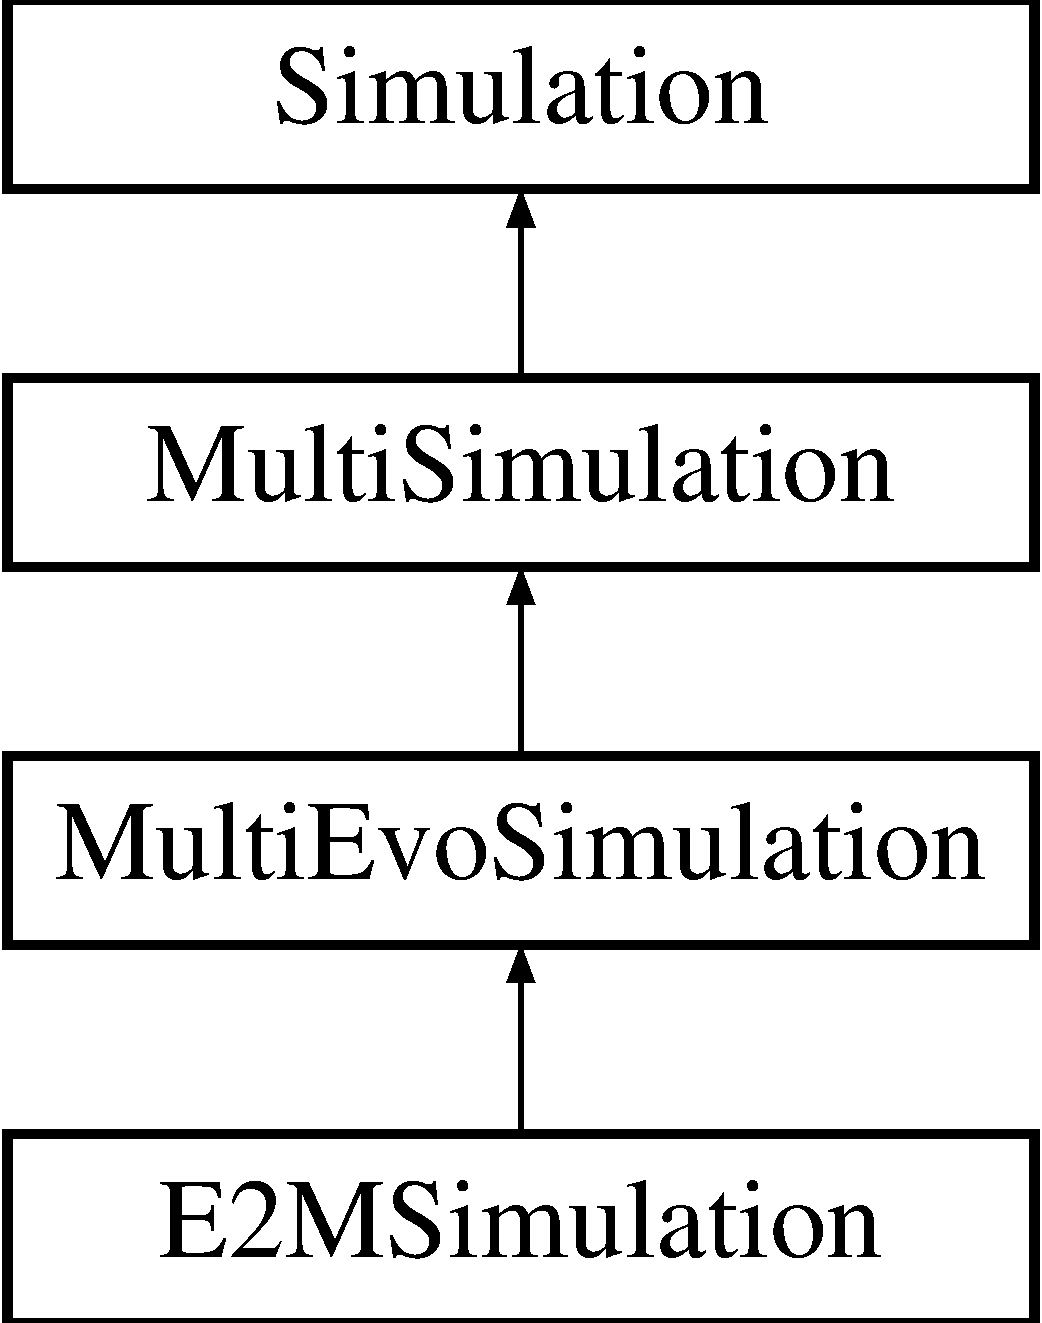
\includegraphics[height=4.000000cm]{classMultiEvoSimulation}
\end{center}
\end{figure}
\subsection*{Public Member Functions}
\begin{DoxyCompactItemize}
\item 
\hypertarget{classMultiEvoSimulation_a39ba876ac0a8771dca1773b37de567dd}{}\label{classMultiEvoSimulation_a39ba876ac0a8771dca1773b37de567dd} 
{\bfseries Multi\+Evo\+Simulation} (vector$<$ \hyperlink{classEnvironment}{Environment} $>$ \+\_\+envs)
\item 
\hypertarget{classMultiEvoSimulation_a965cbb6a21b59b1dcb69a8f7a5cdc63f}{}\label{classMultiEvoSimulation_a965cbb6a21b59b1dcb69a8f7a5cdc63f} 
void {\bfseries set\+Envs} (vector$<$ \hyperlink{classEnvironment}{Environment} $>$ new\+Val)
\item 
\hypertarget{classMultiEvoSimulation_ad15f986cabbba30190e44c503bb02dbd}{}\label{classMultiEvoSimulation_ad15f986cabbba30190e44c503bb02dbd} 
vector$<$ \hyperlink{classEnvironment}{Environment} $>$ $\ast$ {\bfseries get\+Envs} ()
\item 
\hypertarget{classMultiEvoSimulation_af1ed90eb8f214164e5944fa599bebc0f}{}\label{classMultiEvoSimulation_af1ed90eb8f214164e5944fa599bebc0f} 
void {\bfseries add\+Env} (\hyperlink{classEnvironment}{Environment} env)
\item 
\hypertarget{classMultiEvoSimulation_a38cb7774707b70d9d2b08f25132a2ca2}{}\label{classMultiEvoSimulation_a38cb7774707b70d9d2b08f25132a2ca2} 
int {\bfseries get\+Inter\+Save\+Div} ()
\item 
\hypertarget{classMultiEvoSimulation_a325406773501841bbfb51b737ef4fdaf}{}\label{classMultiEvoSimulation_a325406773501841bbfb51b737ef4fdaf} 
void {\bfseries set\+Inter\+Save\+Div} (int new\+Val)
\item 
virtual int \hyperlink{classMultiEvoSimulation_a89c9806ac998c06230cdd41cc6a532bf}{run\+Sim} (int run\+Number)
\begin{DoxyCompactList}\small\item\em Method that runs the main loop of the simulation. \end{DoxyCompactList}\end{DoxyCompactItemize}
\subsection*{Protected Attributes}
\begin{DoxyCompactItemize}
\item 
int \hyperlink{classMultiEvoSimulation_ac9389b3f03afb6195da67337cd1f1957}{inter\+Save\+Div}
\item 
\hypertarget{classMultiEvoSimulation_a17a397017c8b5ea23810bd2f06fac253}{}\label{classMultiEvoSimulation_a17a397017c8b5ea23810bd2f06fac253} 
vector$<$ \hyperlink{classEnvironment}{Environment} $>$ {\bfseries envs}
\end{DoxyCompactItemize}


\subsection{Detailed Description}
Class containing all \hyperlink{classEnvironment}{Environment} objects, as well control-\/flow attributes for the simulation. 

Same as \hyperlink{classEvoSimulation}{Evo\+Simulation}, but for simulations with multiple environments (see also \hyperlink{classMultiSimulation}{Multi\+Simulation}) 

\subsection{Member Function Documentation}
\hypertarget{classMultiEvoSimulation_a89c9806ac998c06230cdd41cc6a532bf}{}\label{classMultiEvoSimulation_a89c9806ac998c06230cdd41cc6a532bf} 
\index{Multi\+Evo\+Simulation@{Multi\+Evo\+Simulation}!run\+Sim@{run\+Sim}}
\index{run\+Sim@{run\+Sim}!Multi\+Evo\+Simulation@{Multi\+Evo\+Simulation}}
\subsubsection{\texorpdfstring{run\+Sim()}{runSim()}}
{\footnotesize\ttfamily int Multi\+Evo\+Simulation\+::run\+Sim (\begin{DoxyParamCaption}\item[{int}]{run\+Number }\end{DoxyParamCaption})\hspace{0.3cm}{\ttfamily [virtual]}}



Method that runs the main loop of the simulation. 


\begin{DoxyParams}{Parameters}
{\em run\+Number} & ID of the current run of the simulation. \\
\hline
\end{DoxyParams}


Reimplemented from \hyperlink{classMultiSimulation_a235347d04fd0c7e1a2e35d7a39e77583}{Multi\+Simulation}.



Reimplemented in \hyperlink{classE2MSimulation_aeac4e92c10f89a5c953ace5b1327d20b}{E2\+M\+Simulation}.



\subsection{Member Data Documentation}
\hypertarget{classMultiEvoSimulation_ac9389b3f03afb6195da67337cd1f1957}{}\label{classMultiEvoSimulation_ac9389b3f03afb6195da67337cd1f1957} 
\index{Multi\+Evo\+Simulation@{Multi\+Evo\+Simulation}!inter\+Save\+Div@{inter\+Save\+Div}}
\index{inter\+Save\+Div@{inter\+Save\+Div}!Multi\+Evo\+Simulation@{Multi\+Evo\+Simulation}}
\subsubsection{\texorpdfstring{inter\+Save\+Div}{interSaveDiv}}
{\footnotesize\ttfamily int Multi\+Evo\+Simulation\+::inter\+Save\+Div\hspace{0.3cm}{\ttfamily [protected]}}

Each how many timestep \hyperlink{classSpecies}{Species} interaction values are saved (in raw\+Save file) 

The documentation for this class was generated from the following files\+:\begin{DoxyCompactItemize}
\item 
\hyperlink{MultiEvoSimulation_8hpp}{Multi\+Evo\+Simulation.\+hpp}\item 
Multi\+Evo\+Simulation.\+cpp\end{DoxyCompactItemize}

\hypertarget{classMultiSimulation}{}\section{Multi\+Simulation Class Reference}
\label{classMultiSimulation}\index{Multi\+Simulation@{Multi\+Simulation}}


Class containing all \hyperlink{classEnvironment}{Environment} objects, as well control-\/flow attributes for the simulation.  




{\ttfamily \#include $<$Multi\+Simulation.\+hpp$>$}

Inheritance diagram for Multi\+Simulation\+:\begin{figure}[H]
\begin{center}
\leavevmode
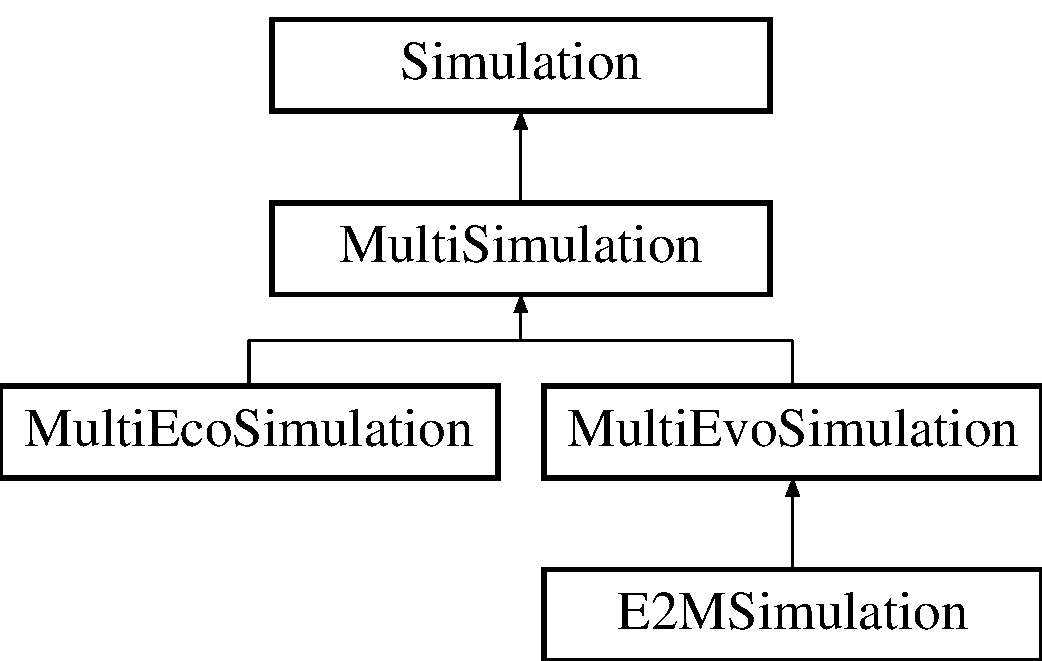
\includegraphics[height=4.000000cm]{classMultiSimulation}
\end{center}
\end{figure}
\subsection*{Public Member Functions}
\begin{DoxyCompactItemize}
\item 
\mbox{\Hypertarget{classMultiSimulation_ad51e5bcf883518c3c817f4d82227f294}\label{classMultiSimulation_ad51e5bcf883518c3c817f4d82227f294}} 
{\bfseries Multi\+Simulation} (vector$<$ \hyperlink{classEnvironment}{Environment} $>$ \+\_\+envs)
\item 
\mbox{\Hypertarget{classMultiSimulation_a04d145935482000983a462bc59ade87c}\label{classMultiSimulation_a04d145935482000983a462bc59ade87c}} 
void {\bfseries set\+Envs} (vector$<$ \hyperlink{classEnvironment}{Environment} $>$ new\+Val)
\item 
\mbox{\Hypertarget{classMultiSimulation_a1ad17e4add05c03fe3719aac54c5d0c3}\label{classMultiSimulation_a1ad17e4add05c03fe3719aac54c5d0c3}} 
vector$<$ \hyperlink{classEnvironment}{Environment} $>$ $\ast$ {\bfseries get\+Envs} ()
\item 
\mbox{\Hypertarget{classMultiSimulation_a445549476e87656b6f153c6e09764b2b}\label{classMultiSimulation_a445549476e87656b6f153c6e09764b2b}} 
void {\bfseries add\+Env} (\hyperlink{classEnvironment}{Environment} env)
\item 
\mbox{\Hypertarget{classMultiSimulation_a589d57167ba82ab6a1d43e49001c669f}\label{classMultiSimulation_a589d57167ba82ab6a1d43e49001c669f}} 
void {\bfseries set\+Num\+Envs} (int new\+Val)
\item 
\mbox{\Hypertarget{classMultiSimulation_a357f60562b2907933dc92638a0fae83b}\label{classMultiSimulation_a357f60562b2907933dc92638a0fae83b}} 
int {\bfseries get\+Num\+Envs} ()
\item 
\mbox{\Hypertarget{classMultiSimulation_a3ae04feb1bf9bae33bf1ed239ff02203}\label{classMultiSimulation_a3ae04feb1bf9bae33bf1ed239ff02203}} 
void {\bfseries set\+Num\+Specs} (int new\+Val)
\item 
\mbox{\Hypertarget{classMultiSimulation_a2e2c2af3cb981335e92bbeb94c56a382}\label{classMultiSimulation_a2e2c2af3cb981335e92bbeb94c56a382}} 
int {\bfseries get\+Num\+Specs} ()
\item 
virtual int \hyperlink{classMultiSimulation_a235347d04fd0c7e1a2e35d7a39e77583}{run\+Sim} (int run\+Number)
\begin{DoxyCompactList}\small\item\em Method that runs the main loop of the simulation. \end{DoxyCompactList}\end{DoxyCompactItemize}
\subsection*{Protected Attributes}
\begin{DoxyCompactItemize}
\item 
\mbox{\Hypertarget{classMultiSimulation_a1a63b241c79c535e6eca8708abd78ba9}\label{classMultiSimulation_a1a63b241c79c535e6eca8708abd78ba9}} 
vector$<$ \hyperlink{classEnvironment}{Environment} $>$ {\bfseries envs}
\item 
int \hyperlink{classMultiSimulation_ac49cc927d6f96d4fda4ff010abc5041a}{num\+Envs}
\item 
int \hyperlink{classMultiSimulation_a383fa1e045cf0e1e7314708c89cb6312}{num\+Specs}
\end{DoxyCompactItemize}


\subsection{Detailed Description}
Class containing all \hyperlink{classEnvironment}{Environment} objects, as well control-\/flow attributes for the simulation. 

The \hyperlink{classMultiSimulation}{Multi\+Simulation} class acts the same way as the \hyperlink{classSimulation}{Simulation} class, but does so on multiple environments. It also gets migrations from each \hyperlink{classEnvironment}{Environment}, and redistributes them to the other Environments. 

\subsection{Member Function Documentation}
\mbox{\Hypertarget{classMultiSimulation_a235347d04fd0c7e1a2e35d7a39e77583}\label{classMultiSimulation_a235347d04fd0c7e1a2e35d7a39e77583}} 
\index{Multi\+Simulation@{Multi\+Simulation}!run\+Sim@{run\+Sim}}
\index{run\+Sim@{run\+Sim}!Multi\+Simulation@{Multi\+Simulation}}
\subsubsection{\texorpdfstring{run\+Sim()}{runSim()}}
{\footnotesize\ttfamily int Multi\+Simulation\+::run\+Sim (\begin{DoxyParamCaption}\item[{int}]{run\+Number }\end{DoxyParamCaption})\hspace{0.3cm}{\ttfamily [virtual]}}



Method that runs the main loop of the simulation. 


\begin{DoxyParams}{Parameters}
{\em run\+Number} & ID of the current run of the simulation. \\
\hline
\end{DoxyParams}


Reimplemented from \hyperlink{classSimulation_a7eb16da89581b496d33b77efbb63b9cd}{Simulation}.



Reimplemented in \hyperlink{classMultiEvoSimulation_a89c9806ac998c06230cdd41cc6a532bf}{Multi\+Evo\+Simulation}, \hyperlink{classE2MSimulation_aeac4e92c10f89a5c953ace5b1327d20b}{E2\+M\+Simulation}, and \hyperlink{classMultiEcoSimulation_ad490e089c083d06d80c62af9e1564ac3}{Multi\+Eco\+Simulation}.



\subsection{Field Documentation}
\mbox{\Hypertarget{classMultiSimulation_ac49cc927d6f96d4fda4ff010abc5041a}\label{classMultiSimulation_ac49cc927d6f96d4fda4ff010abc5041a}} 
\index{Multi\+Simulation@{Multi\+Simulation}!num\+Envs@{num\+Envs}}
\index{num\+Envs@{num\+Envs}!Multi\+Simulation@{Multi\+Simulation}}
\subsubsection{\texorpdfstring{num\+Envs}{numEnvs}}
{\footnotesize\ttfamily int Multi\+Simulation\+::num\+Envs\hspace{0.3cm}{\ttfamily [protected]}}

Total number of environments in simulation \mbox{\Hypertarget{classMultiSimulation_a383fa1e045cf0e1e7314708c89cb6312}\label{classMultiSimulation_a383fa1e045cf0e1e7314708c89cb6312}} 
\index{Multi\+Simulation@{Multi\+Simulation}!num\+Specs@{num\+Specs}}
\index{num\+Specs@{num\+Specs}!Multi\+Simulation@{Multi\+Simulation}}
\subsubsection{\texorpdfstring{num\+Specs}{numSpecs}}
{\footnotesize\ttfamily int Multi\+Simulation\+::num\+Specs\hspace{0.3cm}{\ttfamily [protected]}}

Total number of \hyperlink{classSpecies}{Species} in simulation 

The documentation for this class was generated from the following files\+:\begin{DoxyCompactItemize}
\item 
\hyperlink{MultiSimulation_8hpp}{Multi\+Simulation.\+hpp}\item 
Multi\+Simulation.\+cpp\end{DoxyCompactItemize}

\hypertarget{classNextGen}{}\section{Next\+Gen Class Reference}
\label{classNextGen}\index{Next\+Gen@{Next\+Gen}}


Class containing a single method, used to control transition from one step to the next, and update Species/\+Environemnt attributes (virtual)  




{\ttfamily \#include $<$Next\+Gen.\+hpp$>$}

Inheritance diagram for Next\+Gen\+:\begin{figure}[H]
\begin{center}
\leavevmode
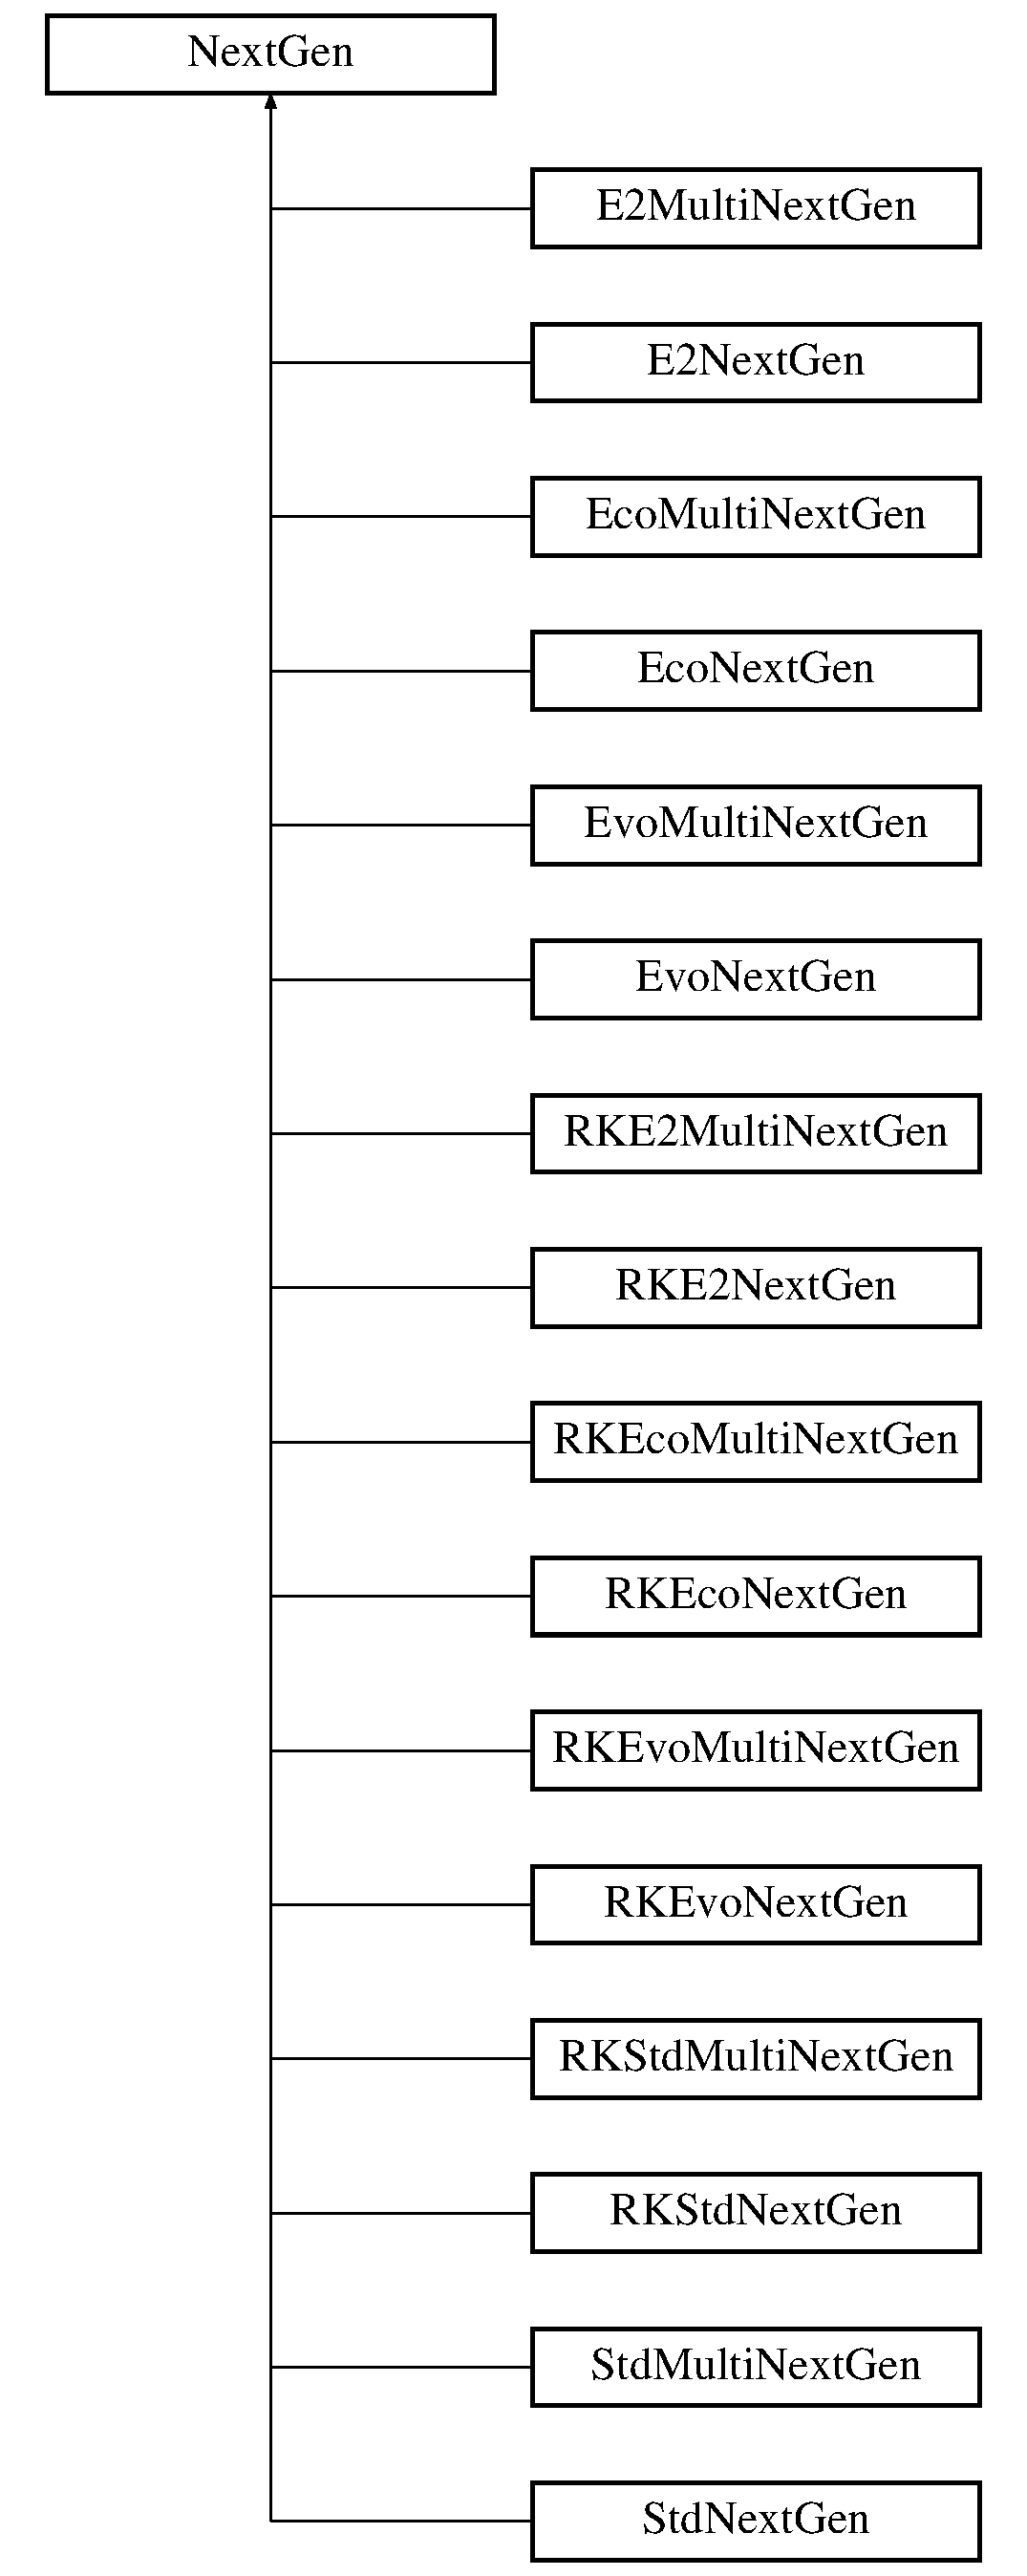
\includegraphics[height=9.000000cm]{classNextGen}
\end{center}
\end{figure}
\subsection*{Public Member Functions}
\begin{DoxyCompactItemize}
\item 
virtual void \hyperlink{classNextGen_aa70da77e0ac03da1bd5414c5e3fd70c0}{get\+Next\+Gen} (int step\+Num, std\+::vector$<$ std\+::unique\+\_\+ptr$<$ \hyperlink{classSpecies}{Species} $>$$>$ $\ast$species\+List, \hyperlink{classEnvironment}{Environment} $\ast$env)=0
\begin{DoxyCompactList}\small\item\em Method used to update Species/\+Environment attributes at each timestep (for details, see documentation of implantations) \end{DoxyCompactList}\end{DoxyCompactItemize}


\subsection{Detailed Description}
Class containing a single method, used to control transition from one step to the next, and update Species/\+Environemnt attributes (virtual) 

An instance of an implementation of this class is owned by each \hyperlink{classEnvironment}{Environment} object, and used to coordinate update in \hyperlink{classSpecies}{Species} density, interactions and environmental parameters (when required). 

\subsection{Member Function Documentation}
\hypertarget{classNextGen_aa70da77e0ac03da1bd5414c5e3fd70c0}{}\label{classNextGen_aa70da77e0ac03da1bd5414c5e3fd70c0} 
\index{Next\+Gen@{Next\+Gen}!get\+Next\+Gen@{get\+Next\+Gen}}
\index{get\+Next\+Gen@{get\+Next\+Gen}!Next\+Gen@{Next\+Gen}}
\subsubsection{\texorpdfstring{get\+Next\+Gen()}{getNextGen()}}
{\footnotesize\ttfamily virtual void Next\+Gen\+::get\+Next\+Gen (\begin{DoxyParamCaption}\item[{int}]{step\+Num,  }\item[{std\+::vector$<$ std\+::unique\+\_\+ptr$<$ \hyperlink{classSpecies}{Species} $>$$>$ $\ast$}]{species\+List,  }\item[{\hyperlink{classEnvironment}{Environment} $\ast$}]{env }\end{DoxyParamCaption})\hspace{0.3cm}{\ttfamily [pure virtual]}}



Method used to update Species/\+Environment attributes at each timestep (for details, see documentation of implantations) 


\begin{DoxyParams}{Parameters}
{\em step\+Num} & Values of the current step \\
\hline
{\em species\+List} & List containing all \hyperlink{classSpecies}{Species} of the environment \\
\hline
{\em env} & Pointer to current environment \\
\hline
\end{DoxyParams}


Implemented in \hyperlink{classE2MultiNextGen_a22721fa0e9c2cbe1de3d0d6bb78932f0}{E2\+Multi\+Next\+Gen}, \hyperlink{classEvoMultiNextGen_acab6fd876dc02feae353b52461b88861}{Evo\+Multi\+Next\+Gen}, \hyperlink{classStdMultiNextGen_a4e3a48cdc731da26abe8b1f32cdbf962}{Std\+Multi\+Next\+Gen}, \hyperlink{classEcoMultiNextGen_a956065141696cac390d8acb8ca5bcccb}{Eco\+Multi\+Next\+Gen}, \hyperlink{classEcoNextGen_a4cb2fccbd3221f41c249c97af461dd3c}{Eco\+Next\+Gen}, \hyperlink{classEvoNextGen_af9ee37c63b6b2c22d27194b6b507c75a}{Evo\+Next\+Gen}, \hyperlink{classStdNextGen_a2253fef9e33f6fe5f2e84f4dc89cfcd2}{Std\+Next\+Gen}, and \hyperlink{classE2NextGen_a2c5d35d9c8f9395cbd58d8fb837a08da}{E2\+Next\+Gen}.



The documentation for this class was generated from the following file\+:\begin{DoxyCompactItemize}
\item 
\hyperlink{NextGen_8hpp}{Next\+Gen.\+hpp}\end{DoxyCompactItemize}

\hypertarget{classNoEvo}{}\section{No\+Evo Class Reference}
\label{classNoEvo}\index{No\+Evo@{No\+Evo}}


Dummy implementation of the \hyperlink{classEvo}{Evo} class.  




{\ttfamily \#include $<$No\+Evo.\+hpp$>$}

Inheritance diagram for No\+Evo\+:\begin{figure}[H]
\begin{center}
\leavevmode
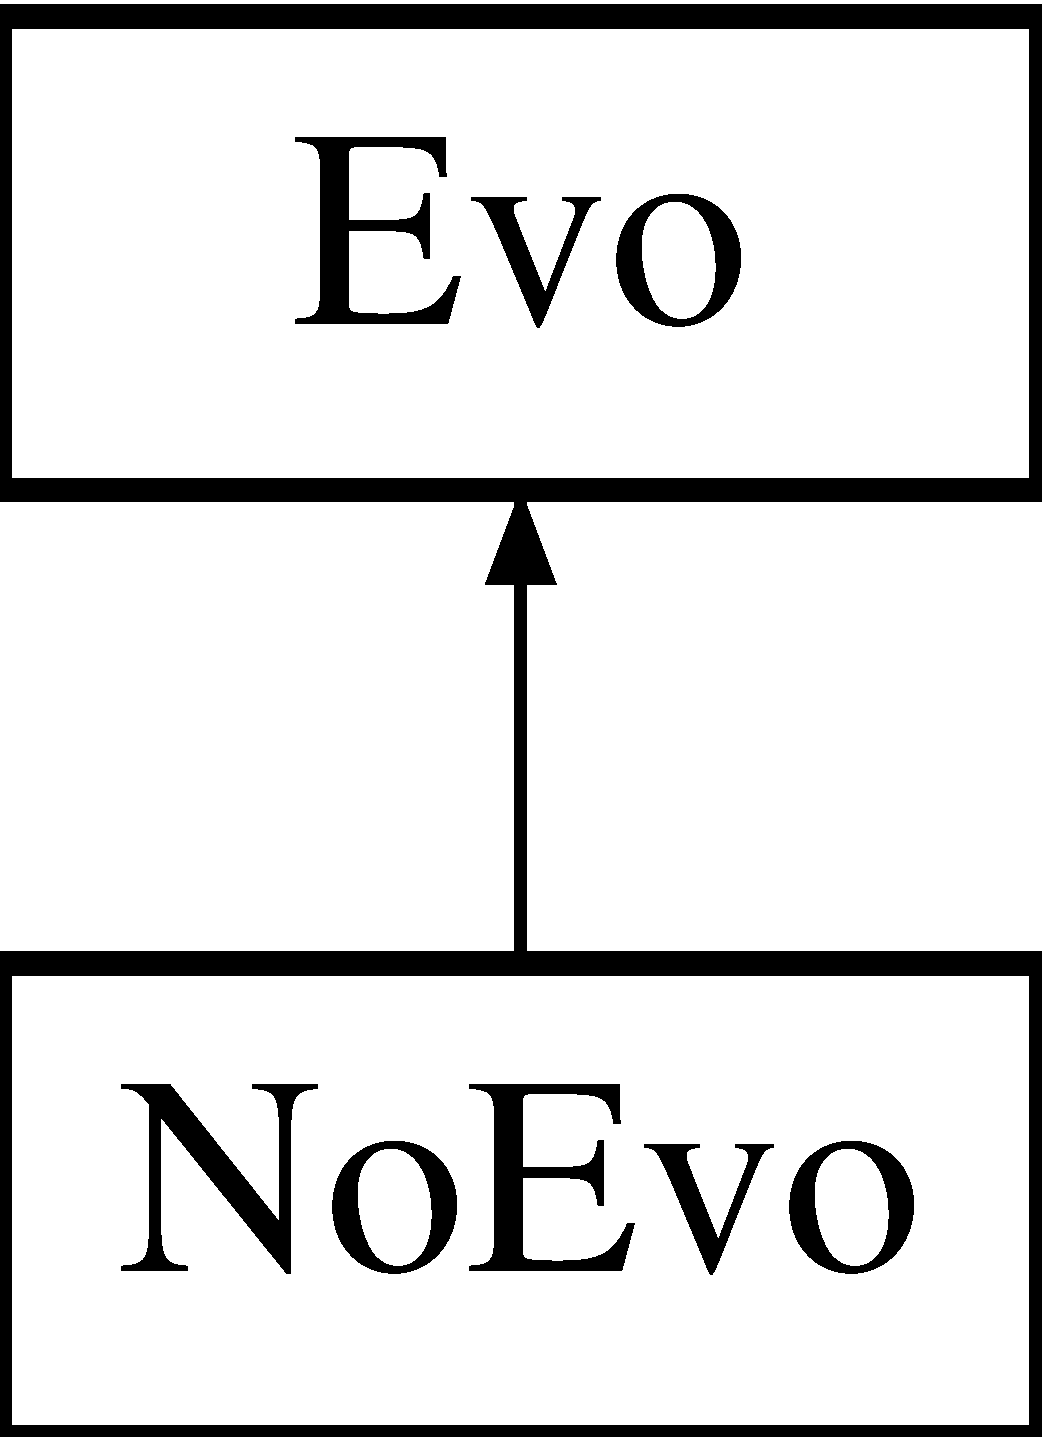
\includegraphics[height=2.000000cm]{classNoEvo}
\end{center}
\end{figure}
\subsection*{Public Member Functions}
\begin{DoxyCompactItemize}
\item 
void \hyperlink{classNoEvo_ad43cc958ff310c4767725c5f4a7e7ac4}{get\+Evo} (vector$<$ unique\+\_\+ptr$<$ \hyperlink{classSpecies}{Species} $>$$>$ $\ast$species\+List, \hyperlink{classSpecies}{Species} $\ast$spec, int resolution)
\begin{DoxyCompactList}\small\item\em Controller method for updating species interactions/optimum. \end{DoxyCompactList}\item 
vector$<$ unique\+\_\+ptr$<$ \hyperlink{classIndividual}{Individual} $>$ $>$ \hyperlink{classNoEvo_a9545e4f14c2038b8b7cab9362cb5fa9a}{get\+Inds} (vector$<$ unique\+\_\+ptr$<$ \hyperlink{classSpecies}{Species} $>$$>$ $\ast$species\+List, \hyperlink{classSpecies}{Species} $\ast$spec, int resolution)
\begin{DoxyCompactList}\small\item\em Method for creating individuals from species. \end{DoxyCompactList}\item 
vector$<$ int $>$ \hyperlink{classNoEvo_ae404207f48accfa7ea9f0022ed1af187}{run\+Selection} (vector$<$ unique\+\_\+ptr$<$ \hyperlink{classIndividual}{Individual} $>$$>$ $\ast$inds, vector$<$ unique\+\_\+ptr$<$ \hyperlink{classSpecies}{Species} $>$$>$ $\ast$species\+List)
\begin{DoxyCompactList}\small\item\em Method that selects surviving/reproducing individuals. \end{DoxyCompactList}\end{DoxyCompactItemize}
\subsection*{Additional Inherited Members}


\subsection{Detailed Description}
Dummy implementation of the \hyperlink{classEvo}{Evo} class. 

Dummy implementaiton of the \hyperlink{classEvo}{Evo} class, given to species in simulations where no evolution occurs. (could also be used to disable evolution in some species) 

\subsection{Member Function Documentation}
\hypertarget{classNoEvo_ad43cc958ff310c4767725c5f4a7e7ac4}{}\label{classNoEvo_ad43cc958ff310c4767725c5f4a7e7ac4} 
\index{No\+Evo@{No\+Evo}!get\+Evo@{get\+Evo}}
\index{get\+Evo@{get\+Evo}!No\+Evo@{No\+Evo}}
\subsubsection{\texorpdfstring{get\+Evo()}{getEvo()}}
{\footnotesize\ttfamily void No\+Evo\+::get\+Evo (\begin{DoxyParamCaption}\item[{vector$<$ unique\+\_\+ptr$<$ \hyperlink{classSpecies}{Species} $>$$>$ $\ast$}]{species\+List,  }\item[{\hyperlink{classSpecies}{Species} $\ast$}]{spec,  }\item[{int}]{resolution }\end{DoxyParamCaption})\hspace{0.3cm}{\ttfamily [inline]}, {\ttfamily [virtual]}}



Controller method for updating species interactions/optimum. 

This method controls the evolutionary process, dividing the species into the right amount of individuals, selecting among them, and updating species interactions and optimum accordingly (for a more detailed description, see implementations).


\begin{DoxyParams}{Parameters}
{\em species\+List} & List containing all (alive) species present in the environment (used to calculate survival/reproduction probability of indivduals). \\
\hline
{\em spec} & \hyperlink{classSpecies}{Species} for which we will calculate evolutionary change (parameters are automatically updated during call). \\
\hline
{\em resolution} & How many discrete individuals are contained in one unit of density. \\
\hline
\end{DoxyParams}


Implements \hyperlink{classEvo_a8c5208c00d1ee2fe9bef41bdd7fe0ab7}{Evo}.

\hypertarget{classNoEvo_a9545e4f14c2038b8b7cab9362cb5fa9a}{}\label{classNoEvo_a9545e4f14c2038b8b7cab9362cb5fa9a} 
\index{No\+Evo@{No\+Evo}!get\+Inds@{get\+Inds}}
\index{get\+Inds@{get\+Inds}!No\+Evo@{No\+Evo}}
\subsubsection{\texorpdfstring{get\+Inds()}{getInds()}}
{\footnotesize\ttfamily vector$<$unique\+\_\+ptr$<$\hyperlink{classIndividual}{Individual}$>$ $>$ No\+Evo\+::get\+Inds (\begin{DoxyParamCaption}\item[{vector$<$ unique\+\_\+ptr$<$ \hyperlink{classSpecies}{Species} $>$$>$ $\ast$}]{species\+List,  }\item[{\hyperlink{classSpecies}{Species} $\ast$}]{spec,  }\item[{int}]{resolution }\end{DoxyParamCaption})\hspace{0.3cm}{\ttfamily [inline]}, {\ttfamily [virtual]}}



Method for creating individuals from species. 

This method divides a species with continous density into a discrete number of individuals {\ttfamily num\+Inds = round(species.\+density) $\ast$ resolution + 1$<$$>$ (+1 to avoid divide-\/by-\/zero errors. For a more detailed description, see implementations).}

{\ttfamily 
\begin{DoxyParams}{Parameters}
{\em species\+List} & List containing all (alive) species present in the environment (used to calculate survival/reproduction probability of indivduals). \\
\hline
{\em spec} & \hyperlink{classSpecies}{Species} from which we will generate individuals. \\
\hline
{\em resolution} & How many discrete individuals are contained in one unit of density. \\
\hline
\end{DoxyParams}
}

Implements \hyperlink{classEvo_a88b5e0b1053cf1b4b473a08e2f03db92}{Evo}.

\hypertarget{classNoEvo_ae404207f48accfa7ea9f0022ed1af187}{}\label{classNoEvo_ae404207f48accfa7ea9f0022ed1af187} 
\index{No\+Evo@{No\+Evo}!run\+Selection@{run\+Selection}}
\index{run\+Selection@{run\+Selection}!No\+Evo@{No\+Evo}}
\subsubsection{\texorpdfstring{run\+Selection()}{runSelection()}}
{\footnotesize\ttfamily vector$<$int$>$ No\+Evo\+::run\+Selection (\begin{DoxyParamCaption}\item[{vector$<$ unique\+\_\+ptr$<$ \hyperlink{classIndividual}{Individual} $>$$>$ $\ast$}]{inds,  }\item[{vector$<$ unique\+\_\+ptr$<$ \hyperlink{classSpecies}{Species} $>$$>$ $\ast$}]{species\+List }\end{DoxyParamCaption})\hspace{0.3cm}{\ttfamily [inline]}, {\ttfamily [virtual]}}



Method that selects surviving/reproducing individuals. 

This method calculates survival/reproduction probability for each individual, and puts the number of existing copies of them in the vector it returns (for a more detailed description, see implementations).


\begin{DoxyParams}{Parameters}
{\em inds} & List containing all individuals that were generated from evolving species. \\
\hline
{\em species\+List} & List containing all (alive) species present in the environment (used to calculate survival/reproduction probability of indivduals). \\
\hline
\end{DoxyParams}


Implements \hyperlink{classEvo_a10ff4eefe3967ff5cf5f820890c18079}{Evo}.



The documentation for this class was generated from the following file\+:\begin{DoxyCompactItemize}
\item 
\hyperlink{NoEvo_8hpp}{No\+Evo.\+hpp}\end{DoxyCompactItemize}

\hypertarget{classRKE2MultiNextGen}{}\section{R\+K\+E2\+Multi\+Next\+Gen Class Reference}
\label{classRKE2MultiNextGen}\index{R\+K\+E2\+Multi\+Next\+Gen@{R\+K\+E2\+Multi\+Next\+Gen}}


Class containing a single method, used to control transition from one step to the next, and update Species/\+Environemnt attributes.  




{\ttfamily \#include $<$R\+K\+E2\+Multi\+Next\+Gen.\+hpp$>$}

Inheritance diagram for R\+K\+E2\+Multi\+Next\+Gen\+:\begin{figure}[H]
\begin{center}
\leavevmode
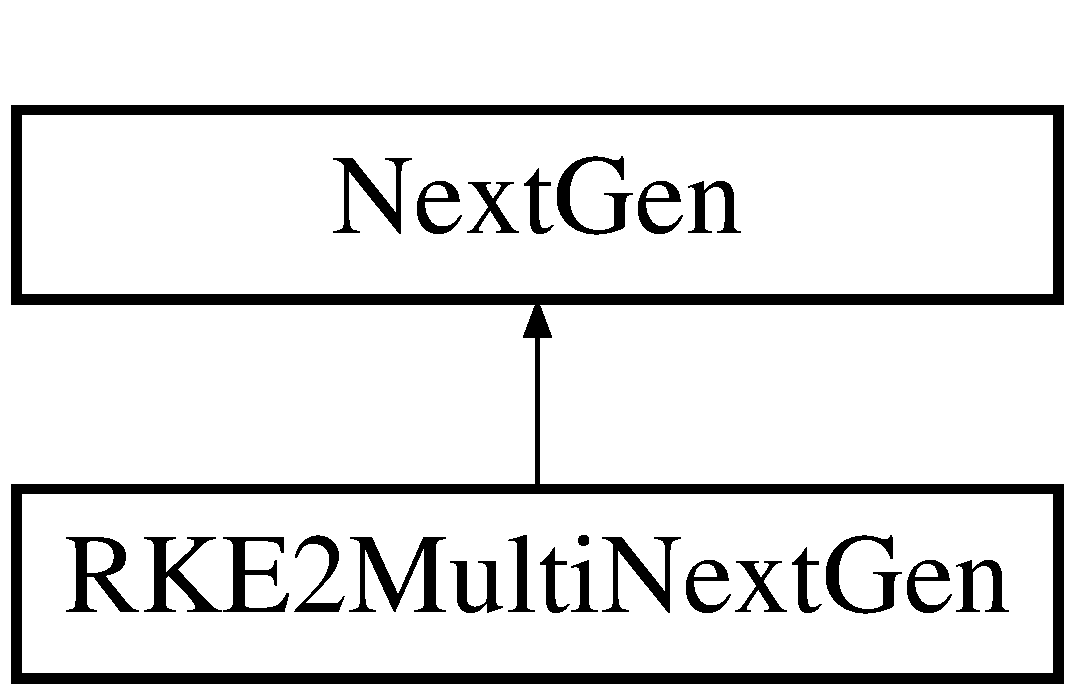
\includegraphics[height=2.000000cm]{classRKE2MultiNextGen}
\end{center}
\end{figure}
\subsection*{Public Member Functions}
\begin{DoxyCompactItemize}
\item 
void \hyperlink{classRKE2MultiNextGen_aec093356f0dd470a1ff985d2ff12c3ff}{get\+Next\+Gen} (int step\+Num, std\+::vector$<$ std\+::unique\+\_\+ptr$<$ \hyperlink{classSpecies}{Species} $>$$>$ $\ast$species\+List, \hyperlink{classEnvironment}{Environment} $\ast$env)
\begin{DoxyCompactList}\small\item\em Method used to update \hyperlink{classSpecies}{Species} density at each timestep. \end{DoxyCompactList}\end{DoxyCompactItemize}


\subsection{Detailed Description}
Class containing a single method, used to control transition from one step to the next, and update Species/\+Environemnt attributes. 

\subsection{Member Function Documentation}
\mbox{\Hypertarget{classRKE2MultiNextGen_aec093356f0dd470a1ff985d2ff12c3ff}\label{classRKE2MultiNextGen_aec093356f0dd470a1ff985d2ff12c3ff}} 
\index{R\+K\+E2\+Multi\+Next\+Gen@{R\+K\+E2\+Multi\+Next\+Gen}!get\+Next\+Gen@{get\+Next\+Gen}}
\index{get\+Next\+Gen@{get\+Next\+Gen}!R\+K\+E2\+Multi\+Next\+Gen@{R\+K\+E2\+Multi\+Next\+Gen}}
\subsubsection{\texorpdfstring{get\+Next\+Gen()}{getNextGen()}}
{\footnotesize\ttfamily void R\+K\+E2\+Multi\+Next\+Gen\+::get\+Next\+Gen (\begin{DoxyParamCaption}\item[{int}]{step\+Num,  }\item[{std\+::vector$<$ std\+::unique\+\_\+ptr$<$ \hyperlink{classSpecies}{Species} $>$$>$ $\ast$}]{species\+List,  }\item[{\hyperlink{classEnvironment}{Environment} $\ast$}]{env }\end{DoxyParamCaption})\hspace{0.3cm}{\ttfamily [virtual]}}



Method used to update \hyperlink{classSpecies}{Species} density at each timestep. 

This method works exactly like the one in \hyperlink{classE2NextGen}{E2\+Next\+Gen}, except that species with {\ttfamily density == 0} are not moved to env.\+dead\+Species, to avoid having to recreate them if a population from said species migrates into environment from somewhere. If migration probability is very low for all species, it might be worth to delete/introduce them each time, since this might take less time than the increased loop time caused by a higher number of species (I\textquotesingle{}d say it depends on the simulation parameters, but I haven\textquotesingle{}t done any performance tests to compare the two methods).


\begin{DoxyParams}{Parameters}
{\em step\+Num} & Values of the current step \\
\hline
{\em species\+List} & List containing all \hyperlink{classSpecies}{Species} of the environment \\
\hline
{\em env} & Pointer to current environment \\
\hline
\end{DoxyParams}


Implements \hyperlink{classNextGen_aa70da77e0ac03da1bd5414c5e3fd70c0}{Next\+Gen}.



The documentation for this class was generated from the following files\+:\begin{DoxyCompactItemize}
\item 
\hyperlink{RKE2MultiNextGen_8hpp}{R\+K\+E2\+Multi\+Next\+Gen.\+hpp}\item 
R\+K\+E2\+Multi\+Next\+Gen.\+cpp\end{DoxyCompactItemize}

\hypertarget{classRKE2NextGen}{}\section{R\+K\+E2\+Next\+Gen Class Reference}
\label{classRKE2NextGen}\index{R\+K\+E2\+Next\+Gen@{R\+K\+E2\+Next\+Gen}}


Class containing a single method, used to control transition from one step to the next, and update Species/\+Environemnt attributes.  




{\ttfamily \#include $<$R\+K\+E2\+Next\+Gen.\+hpp$>$}

Inheritance diagram for R\+K\+E2\+Next\+Gen\+:\begin{figure}[H]
\begin{center}
\leavevmode
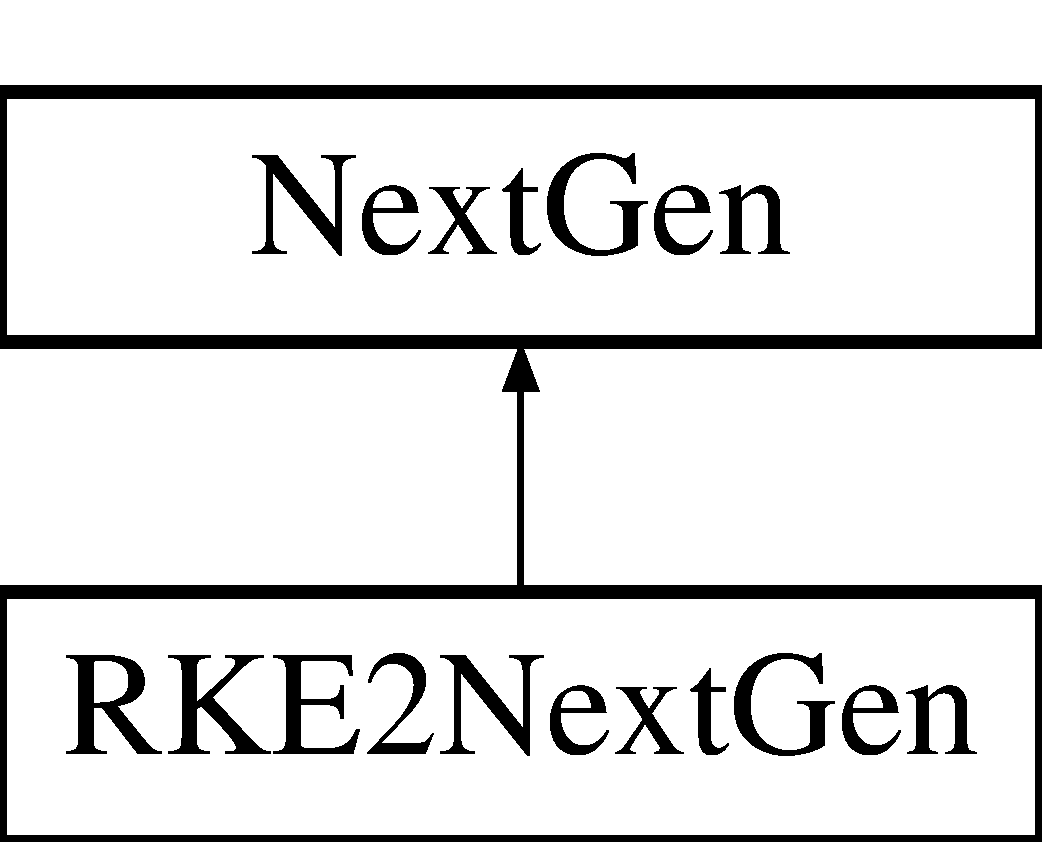
\includegraphics[height=2.000000cm]{classRKE2NextGen}
\end{center}
\end{figure}
\subsection*{Public Member Functions}
\begin{DoxyCompactItemize}
\item 
void \hyperlink{classRKE2NextGen_af91124a237998368739c0bfece6a8725}{get\+Next\+Gen} (int step\+Num, std\+::vector$<$ std\+::unique\+\_\+ptr$<$ \hyperlink{classSpecies}{Species} $>$$>$ $\ast$species\+List, \hyperlink{classEnvironment}{Environment} $\ast$env)
\begin{DoxyCompactList}\small\item\em Method used to update \hyperlink{classSpecies}{Species} density and interactions, as wel as environmental constant at each timestep. \end{DoxyCompactList}\end{DoxyCompactItemize}


\subsection{Detailed Description}
Class containing a single method, used to control transition from one step to the next, and update Species/\+Environemnt attributes. 

\subsection{Member Function Documentation}
\mbox{\Hypertarget{classRKE2NextGen_af91124a237998368739c0bfece6a8725}\label{classRKE2NextGen_af91124a237998368739c0bfece6a8725}} 
\index{R\+K\+E2\+Next\+Gen@{R\+K\+E2\+Next\+Gen}!get\+Next\+Gen@{get\+Next\+Gen}}
\index{get\+Next\+Gen@{get\+Next\+Gen}!R\+K\+E2\+Next\+Gen@{R\+K\+E2\+Next\+Gen}}
\subsubsection{\texorpdfstring{get\+Next\+Gen()}{getNextGen()}}
{\footnotesize\ttfamily void R\+K\+E2\+Next\+Gen\+::get\+Next\+Gen (\begin{DoxyParamCaption}\item[{int}]{step\+Num,  }\item[{std\+::vector$<$ std\+::unique\+\_\+ptr$<$ \hyperlink{classSpecies}{Species} $>$$>$ $\ast$}]{species\+List,  }\item[{\hyperlink{classEnvironment}{Environment} $\ast$}]{env }\end{DoxyParamCaption})\hspace{0.3cm}{\ttfamily [virtual]}}



Method used to update \hyperlink{classSpecies}{Species} density and interactions, as wel as environmental constant at each timestep. 

This method works much in the same way as that of \hyperlink{classStdNextGen}{Std\+Next\+Gen}, but with the added functionality of both \hyperlink{classEcoNextGen}{Eco\+Next\+Gen} and \hyperlink{classEvoNextGen}{Evo\+Next\+Gen}.


\begin{DoxyParams}{Parameters}
{\em step\+Num} & Values of the current step \\
\hline
{\em species\+List} & List containing all \hyperlink{classSpecies}{Species} of the environment \\
\hline
{\em env} & Pointer to current environment \\
\hline
\end{DoxyParams}


Implements \hyperlink{classNextGen_aa70da77e0ac03da1bd5414c5e3fd70c0}{Next\+Gen}.



The documentation for this class was generated from the following files\+:\begin{DoxyCompactItemize}
\item 
\hyperlink{RKE2NextGen_8hpp}{R\+K\+E2\+Next\+Gen.\+hpp}\item 
R\+K\+E2\+Next\+Gen.\+cpp\end{DoxyCompactItemize}

\hypertarget{classRKEcoMultiNextGen}{}\section{R\+K\+Eco\+Multi\+Next\+Gen Class Reference}
\label{classRKEcoMultiNextGen}\index{R\+K\+Eco\+Multi\+Next\+Gen@{R\+K\+Eco\+Multi\+Next\+Gen}}


Class containing a single method, used to control transition from one step to the next, and update Species/\+Environemnt attributes.  




{\ttfamily \#include $<$R\+K\+Eco\+Multi\+Next\+Gen.\+hpp$>$}

Inheritance diagram for R\+K\+Eco\+Multi\+Next\+Gen\+:\begin{figure}[H]
\begin{center}
\leavevmode
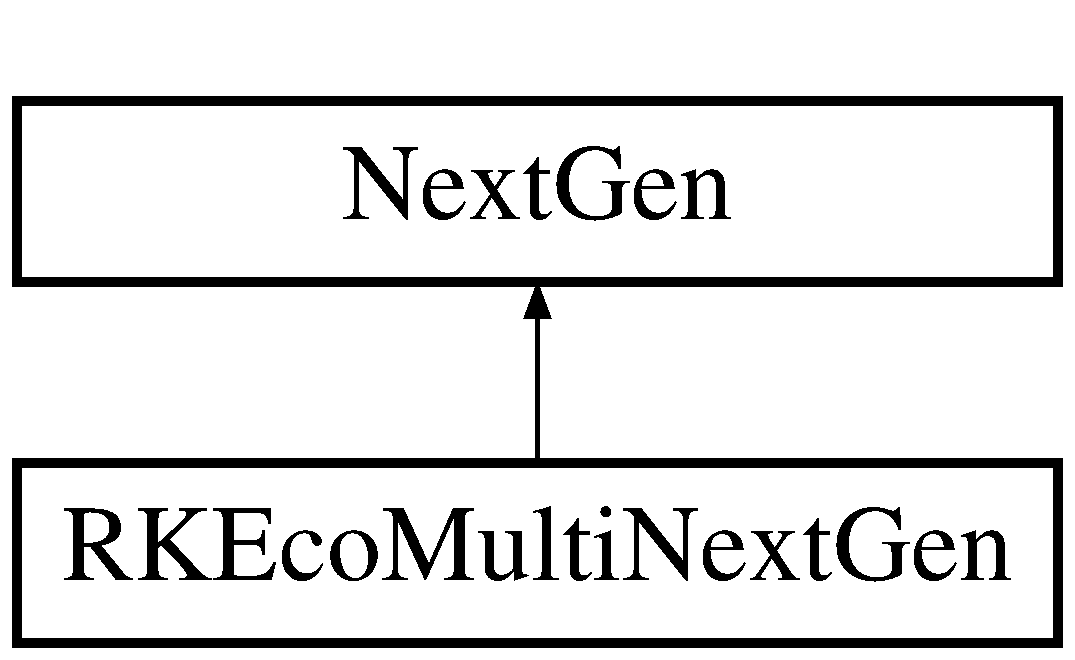
\includegraphics[height=2.000000cm]{classRKEcoMultiNextGen}
\end{center}
\end{figure}
\subsection*{Public Member Functions}
\begin{DoxyCompactItemize}
\item 
void \hyperlink{classRKEcoMultiNextGen_aa6d54650b88870c97b2882dad942c1b1}{get\+Next\+Gen} (int step\+Num, std\+::vector$<$ std\+::unique\+\_\+ptr$<$ \hyperlink{classSpecies}{Species} $>$$>$ $\ast$species\+List, \hyperlink{classEnvironment}{Environment} $\ast$env)
\begin{DoxyCompactList}\small\item\em Method used to update \hyperlink{classSpecies}{Species} density at each timestep. \end{DoxyCompactList}\end{DoxyCompactItemize}


\subsection{Detailed Description}
Class containing a single method, used to control transition from one step to the next, and update Species/\+Environemnt attributes. 

\subsection{Member Function Documentation}
\mbox{\Hypertarget{classRKEcoMultiNextGen_aa6d54650b88870c97b2882dad942c1b1}\label{classRKEcoMultiNextGen_aa6d54650b88870c97b2882dad942c1b1}} 
\index{R\+K\+Eco\+Multi\+Next\+Gen@{R\+K\+Eco\+Multi\+Next\+Gen}!get\+Next\+Gen@{get\+Next\+Gen}}
\index{get\+Next\+Gen@{get\+Next\+Gen}!R\+K\+Eco\+Multi\+Next\+Gen@{R\+K\+Eco\+Multi\+Next\+Gen}}
\subsubsection{\texorpdfstring{get\+Next\+Gen()}{getNextGen()}}
{\footnotesize\ttfamily void R\+K\+Eco\+Multi\+Next\+Gen\+::get\+Next\+Gen (\begin{DoxyParamCaption}\item[{int}]{step\+Num,  }\item[{std\+::vector$<$ std\+::unique\+\_\+ptr$<$ \hyperlink{classSpecies}{Species} $>$$>$ $\ast$}]{species\+List,  }\item[{\hyperlink{classEnvironment}{Environment} $\ast$}]{env }\end{DoxyParamCaption})\hspace{0.3cm}{\ttfamily [virtual]}}



Method used to update \hyperlink{classSpecies}{Species} density at each timestep. 

This method works exactly like the one in \hyperlink{classEcoNextGen}{Eco\+Next\+Gen}, except that species with {\ttfamily density == 0} are not moved to env.\+dead\+Species, to avoid having to recreate them if a population from said species migrates into environment from somewhere. If migration probability is very low for all species, it might be worth to delete/introduce them each time, since this might take less time than the increased loop time caused by a higher number of species (I\textquotesingle{}d say it depends on the simulation parameters, but I haven\textquotesingle{}t done any performance tests to compare the two methods).


\begin{DoxyParams}{Parameters}
{\em step\+Num} & Values of the current step \\
\hline
{\em species\+List} & List containing all \hyperlink{classSpecies}{Species} of the environment \\
\hline
{\em env} & Pointer to current environment \\
\hline
\end{DoxyParams}


Implements \hyperlink{classNextGen_aa70da77e0ac03da1bd5414c5e3fd70c0}{Next\+Gen}.



The documentation for this class was generated from the following files\+:\begin{DoxyCompactItemize}
\item 
\hyperlink{RKEcoMultiNextGen_8hpp}{R\+K\+Eco\+Multi\+Next\+Gen.\+hpp}\item 
R\+K\+Eco\+Multi\+Next\+Gen.\+cpp\end{DoxyCompactItemize}

\hypertarget{classRKEcoNextGen}{}\section{R\+K\+Eco\+Next\+Gen Class Reference}
\label{classRKEcoNextGen}\index{R\+K\+Eco\+Next\+Gen@{R\+K\+Eco\+Next\+Gen}}


Class containing a single method, used to control transition from one step to the next, and update Species/\+Environemnt attributes.  




{\ttfamily \#include $<$R\+K\+Eco\+Next\+Gen.\+hpp$>$}

Inheritance diagram for R\+K\+Eco\+Next\+Gen\+:\begin{figure}[H]
\begin{center}
\leavevmode
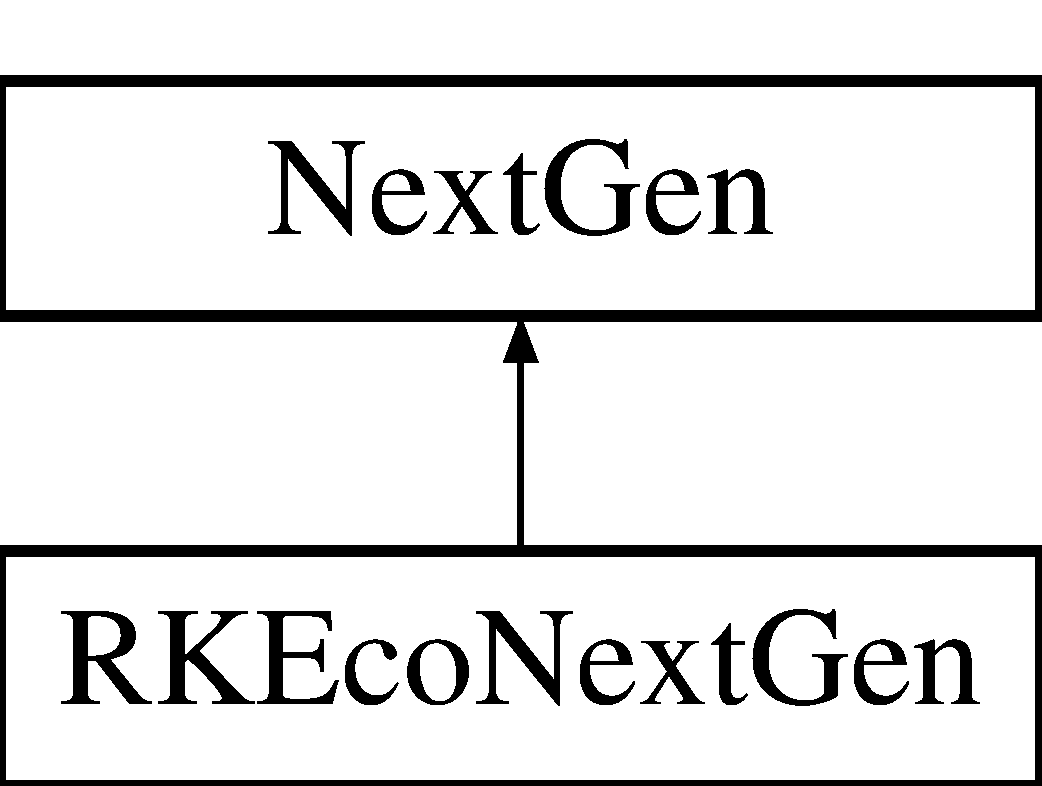
\includegraphics[height=2.000000cm]{classRKEcoNextGen}
\end{center}
\end{figure}
\subsection*{Public Member Functions}
\begin{DoxyCompactItemize}
\item 
void \hyperlink{classRKEcoNextGen_a26225c08c43f3499d98358ff2ecf613f}{get\+Next\+Gen} (int step\+Num, std\+::vector$<$ std\+::unique\+\_\+ptr$<$ \hyperlink{classSpecies}{Species} $>$$>$ $\ast$species\+List, \hyperlink{classEnvironment}{Environment} $\ast$env)
\begin{DoxyCompactList}\small\item\em Method used to update \hyperlink{classSpecies}{Species} density and environmental constant at each timestep. \end{DoxyCompactList}\end{DoxyCompactItemize}


\subsection{Detailed Description}
Class containing a single method, used to control transition from one step to the next, and update Species/\+Environemnt attributes. 

\subsection{Member Function Documentation}
\mbox{\Hypertarget{classRKEcoNextGen_a26225c08c43f3499d98358ff2ecf613f}\label{classRKEcoNextGen_a26225c08c43f3499d98358ff2ecf613f}} 
\index{R\+K\+Eco\+Next\+Gen@{R\+K\+Eco\+Next\+Gen}!get\+Next\+Gen@{get\+Next\+Gen}}
\index{get\+Next\+Gen@{get\+Next\+Gen}!R\+K\+Eco\+Next\+Gen@{R\+K\+Eco\+Next\+Gen}}
\subsubsection{\texorpdfstring{get\+Next\+Gen()}{getNextGen()}}
{\footnotesize\ttfamily void R\+K\+Eco\+Next\+Gen\+::get\+Next\+Gen (\begin{DoxyParamCaption}\item[{int}]{step\+Num,  }\item[{std\+::vector$<$ std\+::unique\+\_\+ptr$<$ \hyperlink{classSpecies}{Species} $>$$>$ $\ast$}]{species\+List,  }\item[{\hyperlink{classEnvironment}{Environment} $\ast$}]{env }\end{DoxyParamCaption})\hspace{0.3cm}{\ttfamily [virtual]}}



Method used to update \hyperlink{classSpecies}{Species} density and environmental constant at each timestep. 

This method works much in the same way as that of \hyperlink{classStdNextGen}{Std\+Next\+Gen}, except that if a call to get\+Random() (heleprs.\+hpp) returns a value smaller than env.\+pert\+Prob, the environmental constant of env will be changed by a random amount drawn form the uniform distribution (env.\+pert\+Range\mbox{[}0\mbox{]}, env.\+pert\+Range\mbox{[}1\mbox{]}) (this happens before species change in densities are calculated). This perturbation is saved in env.\+perturbations.


\begin{DoxyParams}{Parameters}
{\em step\+Num} & Values of the current step \\
\hline
{\em species\+List} & List containing all \hyperlink{classSpecies}{Species} of the environment \\
\hline
{\em env} & Pointer to current environment \\
\hline
\end{DoxyParams}


Implements \hyperlink{classNextGen_aa70da77e0ac03da1bd5414c5e3fd70c0}{Next\+Gen}.



The documentation for this class was generated from the following files\+:\begin{DoxyCompactItemize}
\item 
\hyperlink{RKEcoNextGen_8hpp}{R\+K\+Eco\+Next\+Gen.\+hpp}\item 
R\+K\+Eco\+Next\+Gen.\+cpp\end{DoxyCompactItemize}

\hypertarget{classRKEvoMultiNextGen}{}\section{R\+K\+Evo\+Multi\+Next\+Gen Class Reference}
\label{classRKEvoMultiNextGen}\index{R\+K\+Evo\+Multi\+Next\+Gen@{R\+K\+Evo\+Multi\+Next\+Gen}}


Class containing a single method, used to control transition from one step to the next, and update Species/\+Environemnt attributes.  




{\ttfamily \#include $<$R\+K\+Evo\+Multi\+Next\+Gen.\+hpp$>$}

Inheritance diagram for R\+K\+Evo\+Multi\+Next\+Gen\+:\begin{figure}[H]
\begin{center}
\leavevmode
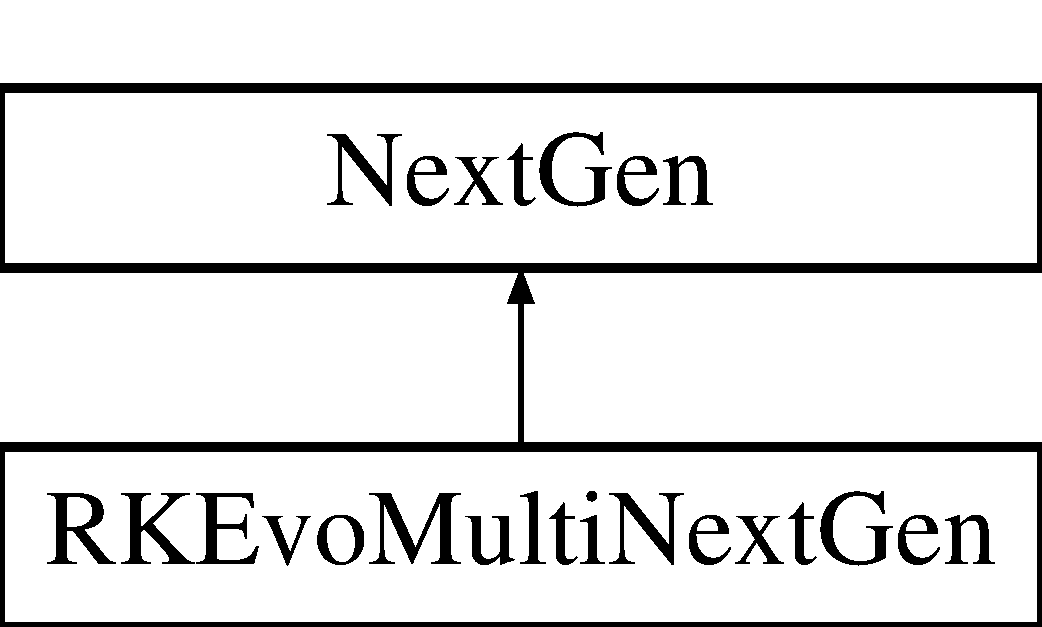
\includegraphics[height=2.000000cm]{classRKEvoMultiNextGen}
\end{center}
\end{figure}
\subsection*{Public Member Functions}
\begin{DoxyCompactItemize}
\item 
void \hyperlink{classRKEvoMultiNextGen_a4b40973651eea9235660af61316b11f6}{get\+Next\+Gen} (int step\+Num, std\+::vector$<$ std\+::unique\+\_\+ptr$<$ \hyperlink{classSpecies}{Species} $>$$>$ $\ast$species\+List, \hyperlink{classEnvironment}{Environment} $\ast$env)
\begin{DoxyCompactList}\small\item\em Method used to update \hyperlink{classSpecies}{Species} density at each timestep. \end{DoxyCompactList}\end{DoxyCompactItemize}


\subsection{Detailed Description}
Class containing a single method, used to control transition from one step to the next, and update Species/\+Environemnt attributes. 

\subsection{Member Function Documentation}
\mbox{\Hypertarget{classRKEvoMultiNextGen_a4b40973651eea9235660af61316b11f6}\label{classRKEvoMultiNextGen_a4b40973651eea9235660af61316b11f6}} 
\index{R\+K\+Evo\+Multi\+Next\+Gen@{R\+K\+Evo\+Multi\+Next\+Gen}!get\+Next\+Gen@{get\+Next\+Gen}}
\index{get\+Next\+Gen@{get\+Next\+Gen}!R\+K\+Evo\+Multi\+Next\+Gen@{R\+K\+Evo\+Multi\+Next\+Gen}}
\subsubsection{\texorpdfstring{get\+Next\+Gen()}{getNextGen()}}
{\footnotesize\ttfamily void R\+K\+Evo\+Multi\+Next\+Gen\+::get\+Next\+Gen (\begin{DoxyParamCaption}\item[{int}]{step\+Num,  }\item[{std\+::vector$<$ std\+::unique\+\_\+ptr$<$ \hyperlink{classSpecies}{Species} $>$$>$ $\ast$}]{species\+List,  }\item[{\hyperlink{classEnvironment}{Environment} $\ast$}]{env }\end{DoxyParamCaption})\hspace{0.3cm}{\ttfamily [virtual]}}



Method used to update \hyperlink{classSpecies}{Species} density at each timestep. 

This method works exactly like the one in \hyperlink{classEvoNextGen}{Evo\+Next\+Gen}, except that species with {\ttfamily density == 0} are not moved to env.\+dead\+Species, to avoid having to recreate them if a population from said species migrates into environment from somewhere. If migration probability is very low for all species, it might be worth to delete/introduce them each time, since this might take less time than the increased loop time caused by a higher number of species (I\textquotesingle{}d say it depends on the simulation parameters, but I haven\textquotesingle{}t done any performance tests to compare the two methods).


\begin{DoxyParams}{Parameters}
{\em step\+Num} & Values of the current step \\
\hline
{\em species\+List} & List containing all \hyperlink{classSpecies}{Species} of the environment \\
\hline
{\em env} & Pointer to current environment \\
\hline
\end{DoxyParams}


Implements \hyperlink{classNextGen_aa70da77e0ac03da1bd5414c5e3fd70c0}{Next\+Gen}.



The documentation for this class was generated from the following files\+:\begin{DoxyCompactItemize}
\item 
\hyperlink{RKEvoMultiNextGen_8hpp}{R\+K\+Evo\+Multi\+Next\+Gen.\+hpp}\item 
R\+K\+Evo\+Multi\+Next\+Gen.\+cpp\end{DoxyCompactItemize}

\hypertarget{classRKEvoNextGen}{}\section{R\+K\+Evo\+Next\+Gen Class Reference}
\label{classRKEvoNextGen}\index{R\+K\+Evo\+Next\+Gen@{R\+K\+Evo\+Next\+Gen}}


Class containing a single method, used to control transition from one step to the next, and update Species/\+Environemnt attributes.  




{\ttfamily \#include $<$R\+K\+Evo\+Next\+Gen.\+hpp$>$}

Inheritance diagram for R\+K\+Evo\+Next\+Gen\+:\begin{figure}[H]
\begin{center}
\leavevmode
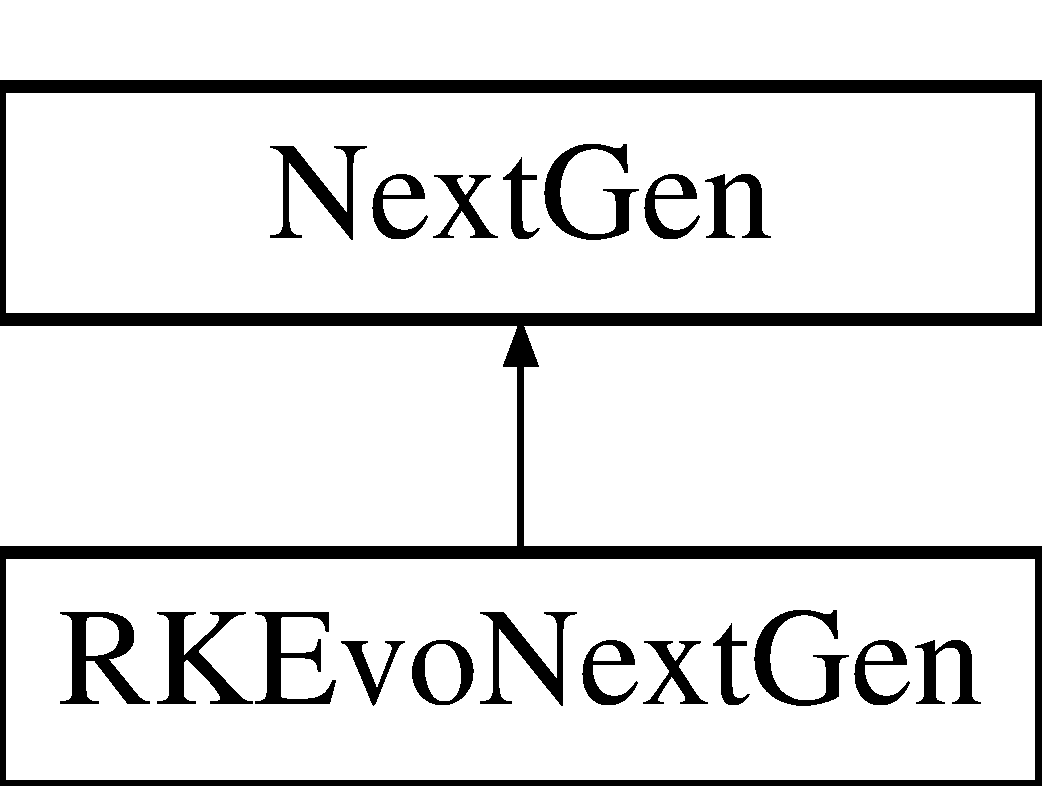
\includegraphics[height=2.000000cm]{classRKEvoNextGen}
\end{center}
\end{figure}
\subsection*{Public Member Functions}
\begin{DoxyCompactItemize}
\item 
void \hyperlink{classRKEvoNextGen_a129cfd567dc8cacd95ca684b1378a43e}{get\+Next\+Gen} (int step\+Num, std\+::vector$<$ std\+::unique\+\_\+ptr$<$ \hyperlink{classSpecies}{Species} $>$$>$ $\ast$species\+List, \hyperlink{classEnvironment}{Environment} $\ast$env)
\begin{DoxyCompactList}\small\item\em Method used to update \hyperlink{classSpecies}{Species} density and interactions at each timestep. \end{DoxyCompactList}\end{DoxyCompactItemize}


\subsection{Detailed Description}
Class containing a single method, used to control transition from one step to the next, and update Species/\+Environemnt attributes. 

\subsection{Member Function Documentation}
\mbox{\Hypertarget{classRKEvoNextGen_a129cfd567dc8cacd95ca684b1378a43e}\label{classRKEvoNextGen_a129cfd567dc8cacd95ca684b1378a43e}} 
\index{R\+K\+Evo\+Next\+Gen@{R\+K\+Evo\+Next\+Gen}!get\+Next\+Gen@{get\+Next\+Gen}}
\index{get\+Next\+Gen@{get\+Next\+Gen}!R\+K\+Evo\+Next\+Gen@{R\+K\+Evo\+Next\+Gen}}
\subsubsection{\texorpdfstring{get\+Next\+Gen()}{getNextGen()}}
{\footnotesize\ttfamily void R\+K\+Evo\+Next\+Gen\+::get\+Next\+Gen (\begin{DoxyParamCaption}\item[{int}]{step\+Num,  }\item[{std\+::vector$<$ std\+::unique\+\_\+ptr$<$ \hyperlink{classSpecies}{Species} $>$$>$ $\ast$}]{species\+List,  }\item[{\hyperlink{classEnvironment}{Environment} $\ast$}]{env }\end{DoxyParamCaption})\hspace{0.3cm}{\ttfamily [virtual]}}



Method used to update \hyperlink{classSpecies}{Species} density and interactions at each timestep. 

This method works much in the same way as that of \hyperlink{classStdNextGen}{Std\+Next\+Gen}, except that after calculating cahnge in \hyperlink{classSpecies}{Species} density for all species (and moving dead species), it calls spec.\+get\+Evo() on each \hyperlink{classSpecies}{Species} where {\ttfamily step\+Numspec.\+evo\+Rate == 0}


\begin{DoxyParams}{Parameters}
{\em step\+Num} & Values of the current step \\
\hline
{\em species\+List} & List containing all \hyperlink{classSpecies}{Species} of the environment \\
\hline
{\em env} & Pointer to current environment \\
\hline
\end{DoxyParams}


Implements \hyperlink{classNextGen_aa70da77e0ac03da1bd5414c5e3fd70c0}{Next\+Gen}.



The documentation for this class was generated from the following files\+:\begin{DoxyCompactItemize}
\item 
\hyperlink{RKEvoNextGen_8hpp}{R\+K\+Evo\+Next\+Gen.\+hpp}\item 
R\+K\+Evo\+Next\+Gen.\+cpp\end{DoxyCompactItemize}

\hypertarget{classRKStdMultiNextGen}{}\section{R\+K\+Std\+Multi\+Next\+Gen Class Reference}
\label{classRKStdMultiNextGen}\index{R\+K\+Std\+Multi\+Next\+Gen@{R\+K\+Std\+Multi\+Next\+Gen}}


Class containing a single method, used to control transition from one step to the next, and update Species/\+Environemnt attributes.  




{\ttfamily \#include $<$R\+K\+Std\+Multi\+Next\+Gen.\+hpp$>$}

Inheritance diagram for R\+K\+Std\+Multi\+Next\+Gen\+:\begin{figure}[H]
\begin{center}
\leavevmode
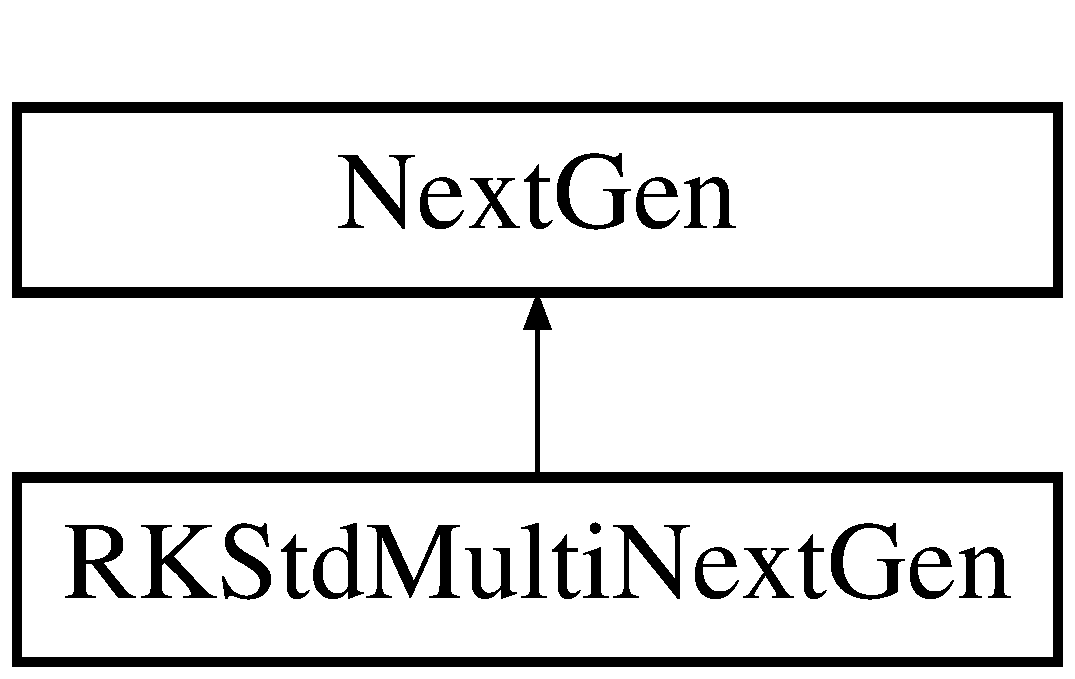
\includegraphics[height=2.000000cm]{classRKStdMultiNextGen}
\end{center}
\end{figure}
\subsection*{Public Member Functions}
\begin{DoxyCompactItemize}
\item 
void \hyperlink{classRKStdMultiNextGen_a78bb057338585e29d4b8fb9962a59a3c}{get\+Next\+Gen} (int step\+Num, std\+::vector$<$ std\+::unique\+\_\+ptr$<$ \hyperlink{classSpecies}{Species} $>$$>$ $\ast$species\+List, \hyperlink{classEnvironment}{Environment} $\ast$env)
\begin{DoxyCompactList}\small\item\em Method used to update \hyperlink{classSpecies}{Species} density at each timestep. \end{DoxyCompactList}\end{DoxyCompactItemize}


\subsection{Detailed Description}
Class containing a single method, used to control transition from one step to the next, and update Species/\+Environemnt attributes. 

\subsection{Member Function Documentation}
\mbox{\Hypertarget{classRKStdMultiNextGen_a78bb057338585e29d4b8fb9962a59a3c}\label{classRKStdMultiNextGen_a78bb057338585e29d4b8fb9962a59a3c}} 
\index{R\+K\+Std\+Multi\+Next\+Gen@{R\+K\+Std\+Multi\+Next\+Gen}!get\+Next\+Gen@{get\+Next\+Gen}}
\index{get\+Next\+Gen@{get\+Next\+Gen}!R\+K\+Std\+Multi\+Next\+Gen@{R\+K\+Std\+Multi\+Next\+Gen}}
\subsubsection{\texorpdfstring{get\+Next\+Gen()}{getNextGen()}}
{\footnotesize\ttfamily void R\+K\+Std\+Multi\+Next\+Gen\+::get\+Next\+Gen (\begin{DoxyParamCaption}\item[{int}]{step\+Num,  }\item[{std\+::vector$<$ std\+::unique\+\_\+ptr$<$ \hyperlink{classSpecies}{Species} $>$$>$ $\ast$}]{species\+List,  }\item[{\hyperlink{classEnvironment}{Environment} $\ast$}]{env }\end{DoxyParamCaption})\hspace{0.3cm}{\ttfamily [virtual]}}



Method used to update \hyperlink{classSpecies}{Species} density at each timestep. 

This method works exactly like the one in \hyperlink{classStdNextGen}{Std\+Next\+Gen}, except that species with {\ttfamily density == 0} are not moved to env.\+dead\+Species, to avoid having to recreate them if a population from said species migrates into environment from somewhere. If migration probability is very low for all species, it might be worth to delete/introduce them each time, since this might take less time than the increased loop time caused by a higher number of species (I\textquotesingle{}d say it depends on the simulation parameters, but I haven\textquotesingle{}t done any performance tests to compare the two methods).


\begin{DoxyParams}{Parameters}
{\em step\+Num} & Values of the current step \\
\hline
{\em species\+List} & List containing all \hyperlink{classSpecies}{Species} of the environment \\
\hline
{\em env} & Pointer to current environment \\
\hline
\end{DoxyParams}


Implements \hyperlink{classNextGen_aa70da77e0ac03da1bd5414c5e3fd70c0}{Next\+Gen}.



The documentation for this class was generated from the following files\+:\begin{DoxyCompactItemize}
\item 
\hyperlink{RKStdMultiNextGen_8hpp}{R\+K\+Std\+Multi\+Next\+Gen.\+hpp}\item 
R\+K\+Std\+Multi\+Next\+Gen.\+cpp\end{DoxyCompactItemize}

\hypertarget{classRKStdNextGen}{}\section{R\+K\+Std\+Next\+Gen Class Reference}
\label{classRKStdNextGen}\index{R\+K\+Std\+Next\+Gen@{R\+K\+Std\+Next\+Gen}}


Class containing a single method, used to control transition from one step to the next, and update Species/\+Environemnt attributes.  




{\ttfamily \#include $<$R\+K\+Std\+Next\+Gen.\+hpp$>$}

Inheritance diagram for R\+K\+Std\+Next\+Gen\+:\begin{figure}[H]
\begin{center}
\leavevmode
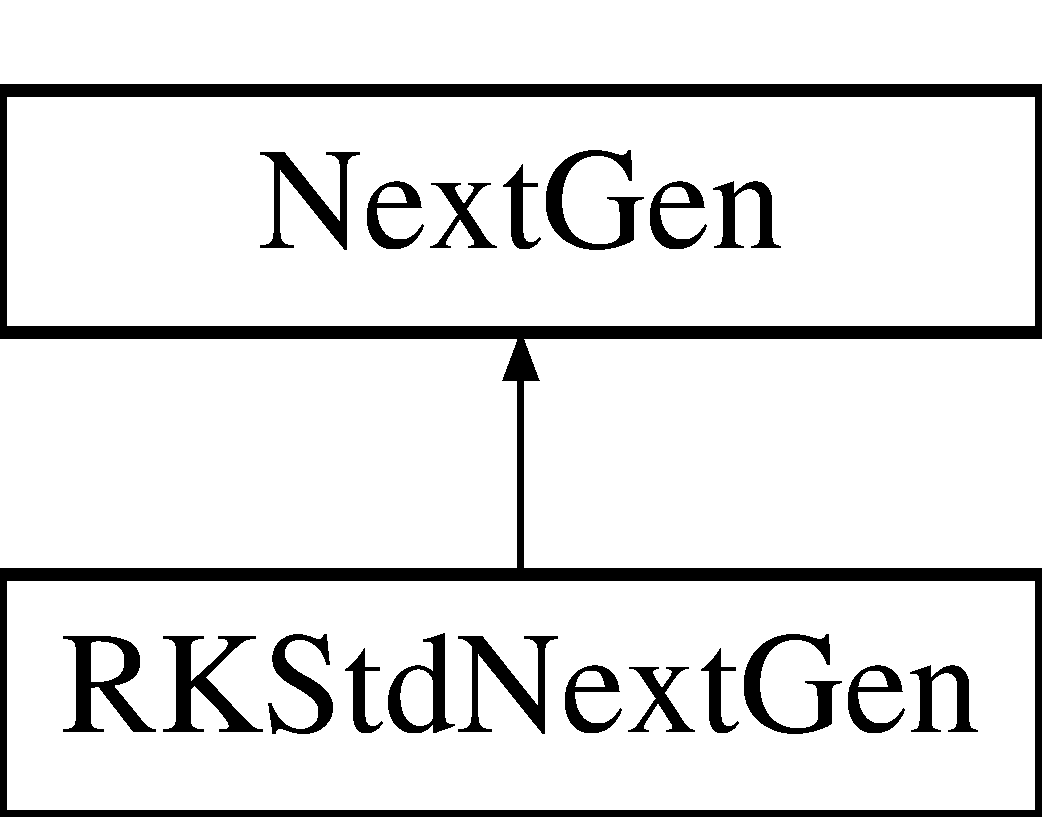
\includegraphics[height=2.000000cm]{classRKStdNextGen}
\end{center}
\end{figure}
\subsection*{Public Member Functions}
\begin{DoxyCompactItemize}
\item 
void \hyperlink{classRKStdNextGen_a6820716e3ffae252ab85591dc19ce337}{get\+Next\+Gen} (int step\+Num, std\+::vector$<$ std\+::unique\+\_\+ptr$<$ \hyperlink{classSpecies}{Species} $>$$>$ $\ast$species\+List, \hyperlink{classEnvironment}{Environment} $\ast$env)
\begin{DoxyCompactList}\small\item\em Method used to update \hyperlink{classSpecies}{Species} density at each timestep. \end{DoxyCompactList}\end{DoxyCompactItemize}


\subsection{Detailed Description}
Class containing a single method, used to control transition from one step to the next, and update Species/\+Environemnt attributes. 

\subsection{Member Function Documentation}
\mbox{\Hypertarget{classRKStdNextGen_a6820716e3ffae252ab85591dc19ce337}\label{classRKStdNextGen_a6820716e3ffae252ab85591dc19ce337}} 
\index{R\+K\+Std\+Next\+Gen@{R\+K\+Std\+Next\+Gen}!get\+Next\+Gen@{get\+Next\+Gen}}
\index{get\+Next\+Gen@{get\+Next\+Gen}!R\+K\+Std\+Next\+Gen@{R\+K\+Std\+Next\+Gen}}
\subsubsection{\texorpdfstring{get\+Next\+Gen()}{getNextGen()}}
{\footnotesize\ttfamily void R\+K\+Std\+Next\+Gen\+::get\+Next\+Gen (\begin{DoxyParamCaption}\item[{int}]{step\+Num,  }\item[{std\+::vector$<$ std\+::unique\+\_\+ptr$<$ \hyperlink{classSpecies}{Species} $>$$>$ $\ast$}]{species\+List,  }\item[{\hyperlink{classEnvironment}{Environment} $\ast$}]{env }\end{DoxyParamCaption})\hspace{0.3cm}{\ttfamily [virtual]}}



Method used to update \hyperlink{classSpecies}{Species} density at each timestep. 

This method first calculates the change in species density for each species, then updates densities for each species. \hyperlink{classSpecies}{Species} whose density is $<$ Envionrment.\+death\+Threshold will have their density set to 0, and be moved from Species\+List to dead\+Species. Used for standard simulation with and without evolution.


\begin{DoxyParams}{Parameters}
{\em step\+Num} & Values of the current step \\
\hline
{\em species\+List} & List containing all \hyperlink{classSpecies}{Species} of the environment \\
\hline
{\em env} & Pointer to current environment \\
\hline
\end{DoxyParams}


Implements \hyperlink{classNextGen_aa70da77e0ac03da1bd5414c5e3fd70c0}{Next\+Gen}.



The documentation for this class was generated from the following files\+:\begin{DoxyCompactItemize}
\item 
\hyperlink{RKStdNextGen_8hpp}{R\+K\+Std\+Next\+Gen.\+hpp}\item 
R\+K\+Std\+Next\+Gen.\+cpp\end{DoxyCompactItemize}

\hypertarget{classSave}{}\section{Save Class Reference}
\label{classSave}\index{Save@{Save}}


Class containing methods responsible for saving any and all aspects of the simulation (except simulation parameters, handled by \hyperlink{interface_8hpp_a573faab2db8e508d0a7189d2bd3fdb4d}{save\+Sim\+Params()} in \hyperlink{interface_8hpp}{interface.\+hpp})  




{\ttfamily \#include $<$Save.\+hpp$>$}

\subsection*{Public Member Functions}
\begin{DoxyCompactItemize}
\item 
\hypertarget{classSave_af60832ca49a38a2569cc78182a2fe8e8}{}\label{classSave_af60832ca49a38a2569cc78182a2fe8e8} 
{\bfseries Save} (bool \+\_\+evo, bool \+\_\+eco, bool \+\_\+multi)
\item 
\hypertarget{classSave_aa59686b2d793182bb2f2d5997f4f5927}{}\label{classSave_aa59686b2d793182bb2f2d5997f4f5927} 
void \hyperlink{classSave_aa59686b2d793182bb2f2d5997f4f5927}{save\+Header} (int run\+Number, \hyperlink{classEnvironment}{Environment} $\ast$env)
\begin{DoxyCompactList}\small\item\em Saves a header of the simulation, indicating which kind of simulation it is, as well as containing information on the \hyperlink{classEnvironment}{Environment}. \end{DoxyCompactList}\item 
void \hyperlink{classSave_ae3cf638e17bf975565ccdd5188a5c156}{save\+All} (int step, vector$<$ unique\+\_\+ptr$<$ \hyperlink{classSpecies}{Species} $>$$>$ $\ast$species\+List, \hyperlink{classEnvironment}{Environment} $\ast$env)
\begin{DoxyCompactList}\small\item\em Saves all pertinent data of the current simulation. \end{DoxyCompactList}\item 
void \hyperlink{classSave_a2e80fc292e7fcea2b327bc7016f34331}{save\+Dens} (int step, vector$<$ unique\+\_\+ptr$<$ \hyperlink{classSpecies}{Species} $>$$>$ $\ast$species\+List, \hyperlink{classEnvironment}{Environment} $\ast$env)
\begin{DoxyCompactList}\small\item\em Saves densities of all species. \end{DoxyCompactList}\item 
void \hyperlink{classSave_a76a537b2f22ae64e63ffaf00e625b955}{save\+Cc} (int step, vector$<$ unique\+\_\+ptr$<$ \hyperlink{classSpecies}{Species} $>$$>$ $\ast$species\+List, \hyperlink{classEnvironment}{Environment} $\ast$env)
\begin{DoxyCompactList}\small\item\em Saves cc (carrying capacity) of all species. \end{DoxyCompactList}\item 
void \hyperlink{classSave_af446df59d19910cd6042680d419b3948}{save\+Inter} (int step, vector$<$ unique\+\_\+ptr$<$ \hyperlink{classSpecies}{Species} $>$$>$ $\ast$species\+List, \hyperlink{classEnvironment}{Environment} $\ast$env)
\begin{DoxyCompactList}\small\item\em Saves interaction values of all species. \end{DoxyCompactList}\item 
void \hyperlink{classSave_a1cea6473b4295efeb65f06895a24f5fb}{save\+Opts} (int step, vector$<$ unique\+\_\+ptr$<$ \hyperlink{classSpecies}{Species} $>$$>$ $\ast$species\+List, \hyperlink{classEnvironment}{Environment} $\ast$env)
\begin{DoxyCompactList}\small\item\em Saves optimums of all species. \end{DoxyCompactList}\item 
void \hyperlink{classSave_a479ae37320e8aaaa98a5636071fb9c59}{complete\+Save} (int run\+Number, int step, vector$<$ unique\+\_\+ptr$<$ \hyperlink{classSpecies}{Species} $>$$>$ $\ast$species\+List, \hyperlink{classEnvironment}{Environment} $\ast$env, int se)
\begin{DoxyCompactList}\small\item\em Makes a complete save of the simulation. \end{DoxyCompactList}\item 
void \hyperlink{classSave_ad66abd97a2e0b7d9dd61cb412cefd01e}{save\+Routes} (vector$<$ unique\+\_\+ptr$<$ \hyperlink{classSpecies}{Species} $>$$>$ $\ast$species\+List, \hyperlink{classEnvironment}{Environment} $\ast$env)
\begin{DoxyCompactList}\small\item\em Saves routes of all species. \end{DoxyCompactList}\item 
void \hyperlink{classSave_a793a85379317ce9e5a08f7155a990fa8}{save\+Evo\+Params} (vector$<$ unique\+\_\+ptr$<$ \hyperlink{classSpecies}{Species} $>$$>$ $\ast$species\+List, \hyperlink{classEnvironment}{Environment} $\ast$env)
\begin{DoxyCompactList}\small\item\em Saves evolution parameters of all species. \end{DoxyCompactList}\item 
void \hyperlink{classSave_a32add352b829b078643bdd1172c18235}{save\+E\+E\+Params} (vector$<$ unique\+\_\+ptr$<$ \hyperlink{classSpecies}{Species} $>$$>$ $\ast$species\+List, \hyperlink{classEnvironment}{Environment} $\ast$env)
\begin{DoxyCompactList}\small\item\em Saves evolution parameters in regards to optimum of all species. \end{DoxyCompactList}\item 
void \hyperlink{classSave_a92d188995ee68892b7631ab67c9b5a18}{save\+Perturbations} (\hyperlink{classEnvironment}{Environment} $\ast$env)
\begin{DoxyCompactList}\small\item\em Saves all perturbations of the \hyperlink{classEnvironment}{Environment} (when they happened, and what value env\+Const had A\+F\+T\+ER they occured) \end{DoxyCompactList}\item 
void \hyperlink{classSave_ad3f864b87a3e5d61b02c251a24a1e030}{save\+Last\+Turn\+Change} (\hyperlink{classEnvironment}{Environment} $\ast$env)
\begin{DoxyCompactList}\small\item\em Saves the total amount of change in density (sum of absolute values) that happened in the envioronment during the last turn of the simulation. \end{DoxyCompactList}\item 
void \hyperlink{classSave_ae7ebfd1c8a546b95e6e99631686dbe41}{save\+DtoI} (vector$<$ unique\+\_\+ptr$<$ \hyperlink{classSpecies}{Species} $>$$>$ $\ast$species\+List, \hyperlink{classEnvironment}{Environment} $\ast$env)
\begin{DoxyCompactList}\small\item\em Saves the density to individuals of all species. \end{DoxyCompactList}\item 
void \hyperlink{classSave_affe306842b77c957b7d83b733fce3bb5}{save\+Alphas} (vector$<$ unique\+\_\+ptr$<$ \hyperlink{classSpecies}{Species} $>$$>$ $\ast$species\+List, \hyperlink{classEnvironment}{Environment} $\ast$env)
\begin{DoxyCompactList}\small\item\em Saves alphas of all species. \end{DoxyCompactList}\item 
void \hyperlink{classSave_ab0b8e1f18d639016fa28f546c60de692}{save\+Betas} (vector$<$ unique\+\_\+ptr$<$ \hyperlink{classSpecies}{Species} $>$$>$ $\ast$species\+List, \hyperlink{classEnvironment}{Environment} $\ast$env)
\begin{DoxyCompactList}\small\item\em Saves betas of all species. \end{DoxyCompactList}\item 
void \hyperlink{classSave_a37a9c18eca58602daae9a9e48345c3ae}{save\+ID} (vector$<$ unique\+\_\+ptr$<$ \hyperlink{classSpecies}{Species} $>$$>$ $\ast$species\+List, \hyperlink{classEnvironment}{Environment} $\ast$env)
\begin{DoxyCompactList}\small\item\em Saves ID of all (live) species (mainly used to re\+Run simulations) \end{DoxyCompactList}\item 
void \hyperlink{classSave_ab9cd9af13ec657f3189974d2d824d5cc}{save\+Final\+Dens} (int step, vector$<$ unique\+\_\+ptr$<$ \hyperlink{classSpecies}{Species} $>$$>$ $\ast$species\+List, vector$<$ unique\+\_\+ptr$<$ \hyperlink{classSpecies}{Species} $>$$>$ $\ast$dead\+Species, \hyperlink{classEnvironment}{Environment} $\ast$env)
\begin{DoxyCompactList}\small\item\em Saves final densities of all species. \end{DoxyCompactList}\item 
\hypertarget{classSave_a700a042e8a6029761f999eb3d373070d}{}\label{classSave_a700a042e8a6029761f999eb3d373070d} 
bool {\bfseries get\+Eco} ()
\end{DoxyCompactItemize}
\subsection*{Protected Attributes}
\begin{DoxyCompactItemize}
\item 
bool \hyperlink{classSave_abaa66610fa9870f1e400a58b8732a996}{evo}
\item 
bool \hyperlink{classSave_a1305b08b2fd9b8fd4add77e3effb594f}{eco}
\item 
bool \hyperlink{classSave_ad1d9db0d8c003efe9e29c497091771e6}{multi}
\end{DoxyCompactItemize}


\subsection{Detailed Description}
Class containing methods responsible for saving any and all aspects of the simulation (except simulation parameters, handled by \hyperlink{interface_8hpp_a573faab2db8e508d0a7189d2bd3fdb4d}{save\+Sim\+Params()} in \hyperlink{interface_8hpp}{interface.\+hpp}) 

This class is responsible for saving simulation results, such as \hyperlink{classSpecies}{Species} density or interaction values. The saves generated with these methods can be used for both statistical analysis of the results, as well as for rerunnning simulations containing \hyperlink{classSpecies}{Species} with the same attributes, but other simulation parameters (e.\+g. desactivatig evolution). The name of the save files are\+:
\begin{DoxyItemize}
\item \char`\"{}raw\+Save\char`\"{}, containing all info on the Environment/\+Species, used by all save methods except \hyperlink{classSave_a479ae37320e8aaaa98a5636071fb9c59}{complete\+Save()} (file name == \hyperlink{classEnvironment_afefeccf87332c116006372e3ee197452}{Environment.\+filename})
\item \char`\"{}complete\+Save\+S\char`\"{}, containing a complete save of the start of the simulation (used to re\+Run simulations) (generated using \hyperlink{classEnvironment_a27a1684288d74f2cabb8cfbd0848b14e}{Environment.\+path})
\item \char`\"{}complete\+Save\+E\char`\"{}, containing a complete save of the end of the simulation (used to re\+Run simulations) (generated using \hyperlink{classEnvironment_a27a1684288d74f2cabb8cfbd0848b14e}{Environment.\+path})
\end{DoxyItemize}

If the simulation has multiple environments, the file names will have the string \char`\"{}\+Env$<$env\+Num$>$\char`\"{} appended (e.\+g. \char`\"{}complete\+Save\+S\+Env2\char`\"{}). For ease of use, this obect contains all methods necessary to save any and all values of the running simulation. Like \hyperlink{classSpecies}{Species} and \hyperlink{classEnvironment}{Environment}, this means that in the case of basic simulations, it uses more space in memory than strictly necessary.

\begin{DoxyWarning}{Warning}
Saves are done directly to disk, and are not buffered in memory. This means high save frequency = high disk access frequency, which can slow down simulations considerably. 
\end{DoxyWarning}


\subsection{Member Function Documentation}
\hypertarget{classSave_a479ae37320e8aaaa98a5636071fb9c59}{}\label{classSave_a479ae37320e8aaaa98a5636071fb9c59} 
\index{Save@{Save}!complete\+Save@{complete\+Save}}
\index{complete\+Save@{complete\+Save}!Save@{Save}}
\subsubsection{\texorpdfstring{complete\+Save()}{completeSave()}}
{\footnotesize\ttfamily void Save\+::complete\+Save (\begin{DoxyParamCaption}\item[{int}]{run\+Number,  }\item[{int}]{step,  }\item[{vector$<$ unique\+\_\+ptr$<$ \hyperlink{classSpecies}{Species} $>$$>$ $\ast$}]{species\+List,  }\item[{\hyperlink{classEnvironment}{Environment} $\ast$}]{env,  }\item[{int}]{se }\end{DoxyParamCaption})}



Makes a complete save of the simulation. 

Complete saves are mainly used to re\+Run a simulation, perhaps after changing some attributes of Species/\+Environment (for more information on loading/re\+Running past simulations, refer to the documentation of \hyperlink{reloadModule_8hpp}{reload\+Module.\+hpp}).


\begin{DoxyParams}{Parameters}
{\em run\+Number} & which run of the simulation we\textquotesingle{}re at. \\
\hline
{\em step} & Step at which the save takes place \\
\hline
{\em species\+List} & List of all \hyperlink{classSpecies}{Species} present in the \hyperlink{classEnvironment}{Environment} \\
\hline
{\em env} & Pointer to the \hyperlink{classEnvironment}{Environment} \\
\hline
{\em se} & Parameter indicating wheter the save happens at the start or the end of a simulation (to determine file name) \\
\hline
\end{DoxyParams}
\hypertarget{classSave_ae3cf638e17bf975565ccdd5188a5c156}{}\label{classSave_ae3cf638e17bf975565ccdd5188a5c156} 
\index{Save@{Save}!save\+All@{save\+All}}
\index{save\+All@{save\+All}!Save@{Save}}
\subsubsection{\texorpdfstring{save\+All()}{saveAll()}}
{\footnotesize\ttfamily void Save\+::save\+All (\begin{DoxyParamCaption}\item[{int}]{step,  }\item[{vector$<$ unique\+\_\+ptr$<$ \hyperlink{classSpecies}{Species} $>$$>$ $\ast$}]{species\+List,  }\item[{\hyperlink{classEnvironment}{Environment} $\ast$}]{env }\end{DoxyParamCaption})}



Saves all pertinent data of the current simulation. 

This method calls all other pertinent \hyperlink{classSave}{Save} methods to make a snapshot of the simulation at a given time (e.\+g. if a simulation doesn\textquotesingle{}t use evolution, the \textquotesingle{}range\textquotesingle{} attribute of the \hyperlink{classSpecies}{Species} class will not be saved, since it is never used).


\begin{DoxyParams}{Parameters}
{\em step} & Step at which the save takes place \\
\hline
{\em species\+List} & List of all \hyperlink{classSpecies}{Species} present in the \hyperlink{classEnvironment}{Environment} \\
\hline
{\em env} & Pointer to the \hyperlink{classEnvironment}{Environment} \\
\hline
\end{DoxyParams}
\hypertarget{classSave_affe306842b77c957b7d83b733fce3bb5}{}\label{classSave_affe306842b77c957b7d83b733fce3bb5} 
\index{Save@{Save}!save\+Alphas@{save\+Alphas}}
\index{save\+Alphas@{save\+Alphas}!Save@{Save}}
\subsubsection{\texorpdfstring{save\+Alphas()}{saveAlphas()}}
{\footnotesize\ttfamily void Save\+::save\+Alphas (\begin{DoxyParamCaption}\item[{vector$<$ unique\+\_\+ptr$<$ \hyperlink{classSpecies}{Species} $>$$>$ $\ast$}]{species\+List,  }\item[{\hyperlink{classEnvironment}{Environment} $\ast$}]{env }\end{DoxyParamCaption})}



Saves alphas of all species. 


\begin{DoxyParams}{Parameters}
{\em species\+List} & List of all \hyperlink{classSpecies}{Species} present in the \hyperlink{classEnvironment}{Environment} \\
\hline
{\em env} & Pointer to the \hyperlink{classEnvironment}{Environment} \\
\hline
\end{DoxyParams}
\hypertarget{classSave_ab0b8e1f18d639016fa28f546c60de692}{}\label{classSave_ab0b8e1f18d639016fa28f546c60de692} 
\index{Save@{Save}!save\+Betas@{save\+Betas}}
\index{save\+Betas@{save\+Betas}!Save@{Save}}
\subsubsection{\texorpdfstring{save\+Betas()}{saveBetas()}}
{\footnotesize\ttfamily void Save\+::save\+Betas (\begin{DoxyParamCaption}\item[{vector$<$ unique\+\_\+ptr$<$ \hyperlink{classSpecies}{Species} $>$$>$ $\ast$}]{species\+List,  }\item[{\hyperlink{classEnvironment}{Environment} $\ast$}]{env }\end{DoxyParamCaption})}



Saves betas of all species. 


\begin{DoxyParams}{Parameters}
{\em species\+List} & List of all \hyperlink{classSpecies}{Species} present in the \hyperlink{classEnvironment}{Environment} \\
\hline
{\em env} & Pointer to the \hyperlink{classEnvironment}{Environment} \\
\hline
\end{DoxyParams}
\hypertarget{classSave_a76a537b2f22ae64e63ffaf00e625b955}{}\label{classSave_a76a537b2f22ae64e63ffaf00e625b955} 
\index{Save@{Save}!save\+Cc@{save\+Cc}}
\index{save\+Cc@{save\+Cc}!Save@{Save}}
\subsubsection{\texorpdfstring{save\+Cc()}{saveCc()}}
{\footnotesize\ttfamily void Save\+::save\+Cc (\begin{DoxyParamCaption}\item[{int}]{step,  }\item[{vector$<$ unique\+\_\+ptr$<$ \hyperlink{classSpecies}{Species} $>$$>$ $\ast$}]{species\+List,  }\item[{\hyperlink{classEnvironment}{Environment} $\ast$}]{env }\end{DoxyParamCaption})}



Saves cc (carrying capacity) of all species. 


\begin{DoxyParams}{Parameters}
{\em step} & Step at which the save takes place \\
\hline
{\em species\+List} & List of all \hyperlink{classSpecies}{Species} present in the \hyperlink{classEnvironment}{Environment} \\
\hline
{\em env} & Pointer to the \hyperlink{classEnvironment}{Environment} \\
\hline
\end{DoxyParams}
\hypertarget{classSave_a2e80fc292e7fcea2b327bc7016f34331}{}\label{classSave_a2e80fc292e7fcea2b327bc7016f34331} 
\index{Save@{Save}!save\+Dens@{save\+Dens}}
\index{save\+Dens@{save\+Dens}!Save@{Save}}
\subsubsection{\texorpdfstring{save\+Dens()}{saveDens()}}
{\footnotesize\ttfamily void Save\+::save\+Dens (\begin{DoxyParamCaption}\item[{int}]{step,  }\item[{vector$<$ unique\+\_\+ptr$<$ \hyperlink{classSpecies}{Species} $>$$>$ $\ast$}]{species\+List,  }\item[{\hyperlink{classEnvironment}{Environment} $\ast$}]{env }\end{DoxyParamCaption})}



Saves densities of all species. 


\begin{DoxyParams}{Parameters}
{\em step} & Step at which the save takes place \\
\hline
{\em species\+List} & List of all \hyperlink{classSpecies}{Species} present in the \hyperlink{classEnvironment}{Environment} \\
\hline
{\em env} & Pointer to the \hyperlink{classEnvironment}{Environment} \\
\hline
\end{DoxyParams}
\hypertarget{classSave_ae7ebfd1c8a546b95e6e99631686dbe41}{}\label{classSave_ae7ebfd1c8a546b95e6e99631686dbe41} 
\index{Save@{Save}!save\+DtoI@{save\+DtoI}}
\index{save\+DtoI@{save\+DtoI}!Save@{Save}}
\subsubsection{\texorpdfstring{save\+Dto\+I()}{saveDtoI()}}
{\footnotesize\ttfamily void Save\+::save\+DtoI (\begin{DoxyParamCaption}\item[{vector$<$ unique\+\_\+ptr$<$ \hyperlink{classSpecies}{Species} $>$$>$ $\ast$}]{species\+List,  }\item[{\hyperlink{classEnvironment}{Environment} $\ast$}]{env }\end{DoxyParamCaption})}



Saves the density to individuals of all species. 


\begin{DoxyParams}{Parameters}
{\em species\+List} & List of all \hyperlink{classSpecies}{Species} present in the \hyperlink{classEnvironment}{Environment} \\
\hline
{\em env} & Pointer to the \hyperlink{classEnvironment}{Environment} \\
\hline
\end{DoxyParams}
\begin{DoxyNote}{Note}
This method is only called when evolution occurs 
\end{DoxyNote}
\hypertarget{classSave_a32add352b829b078643bdd1172c18235}{}\label{classSave_a32add352b829b078643bdd1172c18235} 
\index{Save@{Save}!save\+E\+E\+Params@{save\+E\+E\+Params}}
\index{save\+E\+E\+Params@{save\+E\+E\+Params}!Save@{Save}}
\subsubsection{\texorpdfstring{save\+E\+E\+Params()}{saveEEParams()}}
{\footnotesize\ttfamily void Save\+::save\+E\+E\+Params (\begin{DoxyParamCaption}\item[{vector$<$ unique\+\_\+ptr$<$ \hyperlink{classSpecies}{Species} $>$$>$ $\ast$}]{species\+List,  }\item[{\hyperlink{classEnvironment}{Environment} $\ast$}]{env }\end{DoxyParamCaption})}



Saves evolution parameters in regards to optimum of all species. 


\begin{DoxyParams}{Parameters}
{\em species\+List} & List of all \hyperlink{classSpecies}{Species} present in the \hyperlink{classEnvironment}{Environment} \\
\hline
{\em env} & Pointer to the \hyperlink{classEnvironment}{Environment}\\
\hline
\end{DoxyParams}
\begin{DoxyNote}{Note}
This method is only called when the environmental constant influences \hyperlink{classSpecies}{Species} density change and evolution occurs 
\end{DoxyNote}
\hypertarget{classSave_a793a85379317ce9e5a08f7155a990fa8}{}\label{classSave_a793a85379317ce9e5a08f7155a990fa8} 
\index{Save@{Save}!save\+Evo\+Params@{save\+Evo\+Params}}
\index{save\+Evo\+Params@{save\+Evo\+Params}!Save@{Save}}
\subsubsection{\texorpdfstring{save\+Evo\+Params()}{saveEvoParams()}}
{\footnotesize\ttfamily void Save\+::save\+Evo\+Params (\begin{DoxyParamCaption}\item[{vector$<$ unique\+\_\+ptr$<$ \hyperlink{classSpecies}{Species} $>$$>$ $\ast$}]{species\+List,  }\item[{\hyperlink{classEnvironment}{Environment} $\ast$}]{env }\end{DoxyParamCaption})}



Saves evolution parameters of all species. 


\begin{DoxyParams}{Parameters}
{\em species\+List} & List of all \hyperlink{classSpecies}{Species} present in the \hyperlink{classEnvironment}{Environment} \\
\hline
{\em env} & Pointer to the \hyperlink{classEnvironment}{Environment} \\
\hline
\end{DoxyParams}
\begin{DoxyNote}{Note}
This method is only called when evolution occurs 
\end{DoxyNote}
\hypertarget{classSave_ab9cd9af13ec657f3189974d2d824d5cc}{}\label{classSave_ab9cd9af13ec657f3189974d2d824d5cc} 
\index{Save@{Save}!save\+Final\+Dens@{save\+Final\+Dens}}
\index{save\+Final\+Dens@{save\+Final\+Dens}!Save@{Save}}
\subsubsection{\texorpdfstring{save\+Final\+Dens()}{saveFinalDens()}}
{\footnotesize\ttfamily void Save\+::save\+Final\+Dens (\begin{DoxyParamCaption}\item[{int}]{step,  }\item[{vector$<$ unique\+\_\+ptr$<$ \hyperlink{classSpecies}{Species} $>$$>$ $\ast$}]{species\+List,  }\item[{vector$<$ unique\+\_\+ptr$<$ \hyperlink{classSpecies}{Species} $>$$>$ $\ast$}]{dead\+Species,  }\item[{\hyperlink{classEnvironment}{Environment} $\ast$}]{env }\end{DoxyParamCaption})}



Saves final densities of all species. 

This method is slighlty different from \hyperlink{classSave_a2e80fc292e7fcea2b327bc7016f34331}{save\+Dens()}, so that the python script I use to generate some basic statistics for simulations can differentiate from regular density saves (dead species are also saved for the same reason)


\begin{DoxyParams}{Parameters}
{\em species\+List} & List of all \hyperlink{classSpecies}{Species} present in the \hyperlink{classEnvironment}{Environment} \\
\hline
{\em dead\+Species} & List of all \hyperlink{classSpecies}{Species} where {\ttfamily density == 0} \\
\hline
{\em env} & Pointer to the \hyperlink{classEnvironment}{Environment} \\
\hline
\end{DoxyParams}
\hypertarget{classSave_a37a9c18eca58602daae9a9e48345c3ae}{}\label{classSave_a37a9c18eca58602daae9a9e48345c3ae} 
\index{Save@{Save}!save\+ID@{save\+ID}}
\index{save\+ID@{save\+ID}!Save@{Save}}
\subsubsection{\texorpdfstring{save\+I\+D()}{saveID()}}
{\footnotesize\ttfamily void Save\+::save\+ID (\begin{DoxyParamCaption}\item[{vector$<$ unique\+\_\+ptr$<$ \hyperlink{classSpecies}{Species} $>$$>$ $\ast$}]{species\+List,  }\item[{\hyperlink{classEnvironment}{Environment} $\ast$}]{env }\end{DoxyParamCaption})}



Saves ID of all (live) species (mainly used to re\+Run simulations) 


\begin{DoxyParams}{Parameters}
{\em species\+List} & List of all \hyperlink{classSpecies}{Species} present in the \hyperlink{classEnvironment}{Environment} \\
\hline
{\em env} & Pointer to the \hyperlink{classEnvironment}{Environment} \\
\hline
\end{DoxyParams}
\hypertarget{classSave_af446df59d19910cd6042680d419b3948}{}\label{classSave_af446df59d19910cd6042680d419b3948} 
\index{Save@{Save}!save\+Inter@{save\+Inter}}
\index{save\+Inter@{save\+Inter}!Save@{Save}}
\subsubsection{\texorpdfstring{save\+Inter()}{saveInter()}}
{\footnotesize\ttfamily void Save\+::save\+Inter (\begin{DoxyParamCaption}\item[{int}]{step,  }\item[{vector$<$ unique\+\_\+ptr$<$ \hyperlink{classSpecies}{Species} $>$$>$ $\ast$}]{species\+List,  }\item[{\hyperlink{classEnvironment}{Environment} $\ast$}]{env }\end{DoxyParamCaption})}



Saves interaction values of all species. 


\begin{DoxyParams}{Parameters}
{\em step} & Step at which the save takes place \\
\hline
{\em species\+List} & List of all \hyperlink{classSpecies}{Species} present in the \hyperlink{classEnvironment}{Environment} \\
\hline
{\em env} & Pointer to the \hyperlink{classEnvironment}{Environment} \\
\hline
\end{DoxyParams}
\hypertarget{classSave_ad3f864b87a3e5d61b02c251a24a1e030}{}\label{classSave_ad3f864b87a3e5d61b02c251a24a1e030} 
\index{Save@{Save}!save\+Last\+Turn\+Change@{save\+Last\+Turn\+Change}}
\index{save\+Last\+Turn\+Change@{save\+Last\+Turn\+Change}!Save@{Save}}
\subsubsection{\texorpdfstring{save\+Last\+Turn\+Change()}{saveLastTurnChange()}}
{\footnotesize\ttfamily void Save\+::save\+Last\+Turn\+Change (\begin{DoxyParamCaption}\item[{\hyperlink{classEnvironment}{Environment} $\ast$}]{env }\end{DoxyParamCaption})}



Saves the total amount of change in density (sum of absolute values) that happened in the envioronment during the last turn of the simulation. 


\begin{DoxyParams}{Parameters}
{\em env} & Pointer to the \hyperlink{classEnvironment}{Environment} \\
\hline
\end{DoxyParams}
\hypertarget{classSave_a1cea6473b4295efeb65f06895a24f5fb}{}\label{classSave_a1cea6473b4295efeb65f06895a24f5fb} 
\index{Save@{Save}!save\+Opts@{save\+Opts}}
\index{save\+Opts@{save\+Opts}!Save@{Save}}
\subsubsection{\texorpdfstring{save\+Opts()}{saveOpts()}}
{\footnotesize\ttfamily void Save\+::save\+Opts (\begin{DoxyParamCaption}\item[{int}]{step,  }\item[{vector$<$ unique\+\_\+ptr$<$ \hyperlink{classSpecies}{Species} $>$$>$ $\ast$}]{species\+List,  }\item[{\hyperlink{classEnvironment}{Environment} $\ast$}]{env }\end{DoxyParamCaption})}



Saves optimums of all species. 


\begin{DoxyParams}{Parameters}
{\em step} & Step at which the save takes place \\
\hline
{\em species\+List} & List of all \hyperlink{classSpecies}{Species} present in the \hyperlink{classEnvironment}{Environment} \\
\hline
{\em env} & Pointer to the \hyperlink{classEnvironment}{Environment} \\
\hline
\end{DoxyParams}
\begin{DoxyNote}{Note}
This method is only called when the environmental constant influences \hyperlink{classSpecies}{Species} density change 
\end{DoxyNote}
\hypertarget{classSave_a92d188995ee68892b7631ab67c9b5a18}{}\label{classSave_a92d188995ee68892b7631ab67c9b5a18} 
\index{Save@{Save}!save\+Perturbations@{save\+Perturbations}}
\index{save\+Perturbations@{save\+Perturbations}!Save@{Save}}
\subsubsection{\texorpdfstring{save\+Perturbations()}{savePerturbations()}}
{\footnotesize\ttfamily void Save\+::save\+Perturbations (\begin{DoxyParamCaption}\item[{\hyperlink{classEnvironment}{Environment} $\ast$}]{env }\end{DoxyParamCaption})}



Saves all perturbations of the \hyperlink{classEnvironment}{Environment} (when they happened, and what value env\+Const had A\+F\+T\+ER they occured) 


\begin{DoxyParams}{Parameters}
{\em env} & Pointer to the \hyperlink{classEnvironment}{Environment} \\
\hline
\end{DoxyParams}
\begin{DoxyNote}{Note}
This method is only called when the environmental constant influences \hyperlink{classSpecies}{Species} density change 
\end{DoxyNote}
\hypertarget{classSave_ad66abd97a2e0b7d9dd61cb412cefd01e}{}\label{classSave_ad66abd97a2e0b7d9dd61cb412cefd01e} 
\index{Save@{Save}!save\+Routes@{save\+Routes}}
\index{save\+Routes@{save\+Routes}!Save@{Save}}
\subsubsection{\texorpdfstring{save\+Routes()}{saveRoutes()}}
{\footnotesize\ttfamily void Save\+::save\+Routes (\begin{DoxyParamCaption}\item[{vector$<$ unique\+\_\+ptr$<$ \hyperlink{classSpecies}{Species} $>$$>$ $\ast$}]{species\+List,  }\item[{\hyperlink{classEnvironment}{Environment} $\ast$}]{env }\end{DoxyParamCaption})}



Saves routes of all species. 


\begin{DoxyParams}{Parameters}
{\em step} & Step at which the save takes place \\
\hline
{\em species\+List} & List of all \hyperlink{classSpecies}{Species} present in the \hyperlink{classEnvironment}{Environment} \\
\hline
{\em env} & Pointer to the \hyperlink{classEnvironment}{Environment} \\
\hline
\end{DoxyParams}
\begin{DoxyNote}{Note}
This method is only called when there are multiple environments 
\end{DoxyNote}


\subsection{Member Data Documentation}
\hypertarget{classSave_a1305b08b2fd9b8fd4add77e3effb594f}{}\label{classSave_a1305b08b2fd9b8fd4add77e3effb594f} 
\index{Save@{Save}!eco@{eco}}
\index{eco@{eco}!Save@{Save}}
\subsubsection{\texorpdfstring{eco}{eco}}
{\footnotesize\ttfamily bool Save\+::eco\hspace{0.3cm}{\ttfamily [protected]}}

Used to determine wether to save parameters relating to environmental constant \hypertarget{classSave_abaa66610fa9870f1e400a58b8732a996}{}\label{classSave_abaa66610fa9870f1e400a58b8732a996} 
\index{Save@{Save}!evo@{evo}}
\index{evo@{evo}!Save@{Save}}
\subsubsection{\texorpdfstring{evo}{evo}}
{\footnotesize\ttfamily bool Save\+::evo\hspace{0.3cm}{\ttfamily [protected]}}

Used to determine wether to save parameters relating to evolution \hypertarget{classSave_ad1d9db0d8c003efe9e29c497091771e6}{}\label{classSave_ad1d9db0d8c003efe9e29c497091771e6} 
\index{Save@{Save}!multi@{multi}}
\index{multi@{multi}!Save@{Save}}
\subsubsection{\texorpdfstring{multi}{multi}}
{\footnotesize\ttfamily bool Save\+::multi\hspace{0.3cm}{\ttfamily [protected]}}

Used to determine wether to save parameters relating to multi-\/environment simulations 

The documentation for this class was generated from the following files\+:\begin{DoxyCompactItemize}
\item 
\hyperlink{Save_8hpp}{Save.\+hpp}\item 
Save.\+cpp\end{DoxyCompactItemize}

\hypertarget{structsimParams}{}\section{sim\+Params Struct Reference}
\label{structsimParams}\index{sim\+Params@{sim\+Params}}


A structure that contains all the information necessary to generate a simulation.  




{\ttfamily \#include $<$interface.\+hpp$>$}

\subsection*{Data Fields}
\begin{DoxyCompactItemize}
\item 
bool \hyperlink{structsimParams_a7b06eae32b1691cb52bfc4a7e135f589}{complete\+End} = false
\item 
bool \hyperlink{structsimParams_ad96e572c78fc800e13936b937f3addca}{complete\+Start} = false
\item 
\mbox{\Hypertarget{structsimParams_ab73f45f2fefc0df819177fac8ecbdb00}\label{structsimParams_ab73f45f2fefc0df819177fac8ecbdb00}} 
bool {\bfseries rk} = false
\item 
double \hyperlink{structsimParams_a459d8e2a902ef06f2e6ccce91a5f40bc}{inter\+Range} \mbox{[}2\mbox{]}
\item 
double \hyperlink{structsimParams_a48b3258fb2eabaf36a4392a3be846366}{dens\+Range} \mbox{[}2\mbox{]}
\item 
double \hyperlink{structsimParams_a2674f228bf6b33bf35dc6d1cfb6befba}{alpha\+Range} \mbox{[}2\mbox{]}
\item 
double \hyperlink{structsimParams_a676b73cd7d60743090c9f2b4c166c083}{beta\+Range} \mbox{[}2\mbox{]}
\item 
double \hyperlink{structsimParams_a730247ea2898e90b85dd99c55d8a18e3}{cc\+Range} \mbox{[}2\mbox{]}
\item 
double \hyperlink{structsimParams_a169d5e6c66da8b477bb7e384fe4c90b8}{opt\+Range\+Spec} \mbox{[}2\mbox{]}
\item 
double \hyperlink{structsimParams_ab59d469330753aebd7ce7ab893a6eda4}{opt\+Range\+Env} \mbox{[}2\mbox{]}
\item 
double \hyperlink{structsimParams_a328c95295bd7872174fa9a22c9c402cd}{evo\+Range\+Range} \mbox{[}2\mbox{]}
\item 
double \hyperlink{structsimParams_a2822e99362ed71f123e812a8fd9ad443}{opt\+Evo\+Range} \mbox{[}2\mbox{]}
\item 
double \hyperlink{structsimParams_a4a67c773b31598604c56efc130a69945}{mig\+Prob\+Range} \mbox{[}2\mbox{]}
\item 
double \hyperlink{structsimParams_a2486796d56e9fbe5d9f2dbd507a6ce5d}{mig\+Size\+Range} \mbox{[}2\mbox{]}
\item 
double \hyperlink{structsimParams_a9b9d328e41381a83004b5fa062248fc7}{pert\+Range} \mbox{[}2\mbox{]}
\item 
double \hyperlink{structsimParams_a1d2d1053c8780cea2eb1f703b1bcafd0}{delta}
\item 
double \hyperlink{structsimParams_aec04ef00f25e3bb5585a7a4b50c32b9a}{death\+Threshold}
\item 
double \hyperlink{structsimParams_aa07ddc0d55d057a586dc98ffd113e064}{perturbation\+Prob}
\item 
int \hyperlink{structsimParams_ace2069f1d65920fe32e4236c12e91ea9}{gen\+Time\+Range} \mbox{[}2\mbox{]}
\item 
int \hyperlink{structsimParams_a4121b97ac4b40f6d309693847309ce6b}{evo\+Res\+Range} \mbox{[}2\mbox{]}
\item 
vector$<$ int $>$ \hyperlink{structsimParams_aede5150c0b33bacae326638341a4e906}{specs\+Per\+Env}
\item 
int \hyperlink{structsimParams_a83b3c9f8e5dee0b7b4e63a17dc2646bd}{num\+Specs}
\item 
int \hyperlink{structsimParams_a027234312109ab21e3f8dacda4039c9f}{num\+Steps}
\item 
int \hyperlink{structsimParams_ad9fb5fcc3890d022270dbe00ec3a7c1e}{save\+Div}
\item 
int \hyperlink{structsimParams_a2114f7c6664772255e0e8afcf9334ebf}{inter\+Save\+Div}
\item 
int \hyperlink{structsimParams_a5d284deecb9cbd1b2680670822cae29a}{num\+Envs}
\item 
char \hyperlink{structsimParams_ac1a96378c33a770e34ffba03498735c9}{eco}
\item 
char \hyperlink{structsimParams_a26cb871bb244145cf0b4d1754864f276}{evo}
\item 
char \hyperlink{structsimParams_a2c0a57da585258a84362a2c297ee44cb}{multi}
\end{DoxyCompactItemize}


\subsection{Detailed Description}
A structure that contains all the information necessary to generate a simulation. 

\subsection{Field Documentation}
\mbox{\Hypertarget{structsimParams_a2674f228bf6b33bf35dc6d1cfb6befba}\label{structsimParams_a2674f228bf6b33bf35dc6d1cfb6befba}} 
\index{sim\+Params@{sim\+Params}!alpha\+Range@{alpha\+Range}}
\index{alpha\+Range@{alpha\+Range}!sim\+Params@{sim\+Params}}
\subsubsection{\texorpdfstring{alpha\+Range}{alphaRange}}
{\footnotesize\ttfamily double sim\+Params\+::alpha\+Range\mbox{[}2\mbox{]}}

Unfirom range from which \hyperlink{classSpecies}{Species} alpha values are drawn \mbox{\Hypertarget{structsimParams_a676b73cd7d60743090c9f2b4c166c083}\label{structsimParams_a676b73cd7d60743090c9f2b4c166c083}} 
\index{sim\+Params@{sim\+Params}!beta\+Range@{beta\+Range}}
\index{beta\+Range@{beta\+Range}!sim\+Params@{sim\+Params}}
\subsubsection{\texorpdfstring{beta\+Range}{betaRange}}
{\footnotesize\ttfamily double sim\+Params\+::beta\+Range\mbox{[}2\mbox{]}}

Unfirom range from which \hyperlink{classSpecies}{Species} beta values are drawn \mbox{\Hypertarget{structsimParams_a730247ea2898e90b85dd99c55d8a18e3}\label{structsimParams_a730247ea2898e90b85dd99c55d8a18e3}} 
\index{sim\+Params@{sim\+Params}!cc\+Range@{cc\+Range}}
\index{cc\+Range@{cc\+Range}!sim\+Params@{sim\+Params}}
\subsubsection{\texorpdfstring{cc\+Range}{ccRange}}
{\footnotesize\ttfamily double sim\+Params\+::cc\+Range\mbox{[}2\mbox{]}}

Unfirom range from which \hyperlink{classSpecies}{Species} carrying capacity (cc) values are drawn \mbox{\Hypertarget{structsimParams_a7b06eae32b1691cb52bfc4a7e135f589}\label{structsimParams_a7b06eae32b1691cb52bfc4a7e135f589}} 
\index{sim\+Params@{sim\+Params}!complete\+End@{complete\+End}}
\index{complete\+End@{complete\+End}!sim\+Params@{sim\+Params}}
\subsubsection{\texorpdfstring{complete\+End}{completeEnd}}
{\footnotesize\ttfamily bool sim\+Params\+::complete\+End = false}

Bool deciding wether or not there are complete saves made at the end of a simulation \mbox{\Hypertarget{structsimParams_ad96e572c78fc800e13936b937f3addca}\label{structsimParams_ad96e572c78fc800e13936b937f3addca}} 
\index{sim\+Params@{sim\+Params}!complete\+Start@{complete\+Start}}
\index{complete\+Start@{complete\+Start}!sim\+Params@{sim\+Params}}
\subsubsection{\texorpdfstring{complete\+Start}{completeStart}}
{\footnotesize\ttfamily bool sim\+Params\+::complete\+Start = false}

Bool deciding wether or not there are complete saves made at the start of a simulation \mbox{\Hypertarget{structsimParams_aec04ef00f25e3bb5585a7a4b50c32b9a}\label{structsimParams_aec04ef00f25e3bb5585a7a4b50c32b9a}} 
\index{sim\+Params@{sim\+Params}!death\+Threshold@{death\+Threshold}}
\index{death\+Threshold@{death\+Threshold}!sim\+Params@{sim\+Params}}
\subsubsection{\texorpdfstring{death\+Threshold}{deathThreshold}}
{\footnotesize\ttfamily double sim\+Params\+::death\+Threshold}

Density below which species a\+Se considered extinct (-\/$>$ \hyperlink{classSpecies}{Species} density is set to 0) \mbox{\Hypertarget{structsimParams_a1d2d1053c8780cea2eb1f703b1bcafd0}\label{structsimParams_a1d2d1053c8780cea2eb1f703b1bcafd0}} 
\index{sim\+Params@{sim\+Params}!delta@{delta}}
\index{delta@{delta}!sim\+Params@{sim\+Params}}
\subsubsection{\texorpdfstring{delta}{delta}}
{\footnotesize\ttfamily double sim\+Params\+::delta}

Step size in the explicit Euler Scheme \mbox{\Hypertarget{structsimParams_a48b3258fb2eabaf36a4392a3be846366}\label{structsimParams_a48b3258fb2eabaf36a4392a3be846366}} 
\index{sim\+Params@{sim\+Params}!dens\+Range@{dens\+Range}}
\index{dens\+Range@{dens\+Range}!sim\+Params@{sim\+Params}}
\subsubsection{\texorpdfstring{dens\+Range}{densRange}}
{\footnotesize\ttfamily double sim\+Params\+::dens\+Range\mbox{[}2\mbox{]}}

Unfirom range from which \hyperlink{classSpecies}{Species} density values are drawn \mbox{\Hypertarget{structsimParams_ac1a96378c33a770e34ffba03498735c9}\label{structsimParams_ac1a96378c33a770e34ffba03498735c9}} 
\index{sim\+Params@{sim\+Params}!eco@{eco}}
\index{eco@{eco}!sim\+Params@{sim\+Params}}
\subsubsection{\texorpdfstring{eco}{eco}}
{\footnotesize\ttfamily char sim\+Params\+::eco}

Wether or not the environmental constant is taken into account (\textquotesingle{}y\textquotesingle{} or \textquotesingle{}n\textquotesingle{}) \mbox{\Hypertarget{structsimParams_a26cb871bb244145cf0b4d1754864f276}\label{structsimParams_a26cb871bb244145cf0b4d1754864f276}} 
\index{sim\+Params@{sim\+Params}!evo@{evo}}
\index{evo@{evo}!sim\+Params@{sim\+Params}}
\subsubsection{\texorpdfstring{evo}{evo}}
{\footnotesize\ttfamily char sim\+Params\+::evo}

Wether or not evolution is on in this simulation (\textquotesingle{}y\textquotesingle{} or \textquotesingle{}n\textquotesingle{}) \mbox{\Hypertarget{structsimParams_a328c95295bd7872174fa9a22c9c402cd}\label{structsimParams_a328c95295bd7872174fa9a22c9c402cd}} 
\index{sim\+Params@{sim\+Params}!evo\+Range\+Range@{evo\+Range\+Range}}
\index{evo\+Range\+Range@{evo\+Range\+Range}!sim\+Params@{sim\+Params}}
\subsubsection{\texorpdfstring{evo\+Range\+Range}{evoRangeRange}}
{\footnotesize\ttfamily double sim\+Params\+::evo\+Range\+Range\mbox{[}2\mbox{]}}

Unfirom range from which evolution ranges for interaction values are drawn (see \hyperlink{classEvo}{Evo}) \mbox{\Hypertarget{structsimParams_a4121b97ac4b40f6d309693847309ce6b}\label{structsimParams_a4121b97ac4b40f6d309693847309ce6b}} 
\index{sim\+Params@{sim\+Params}!evo\+Res\+Range@{evo\+Res\+Range}}
\index{evo\+Res\+Range@{evo\+Res\+Range}!sim\+Params@{sim\+Params}}
\subsubsection{\texorpdfstring{evo\+Res\+Range}{evoResRange}}
{\footnotesize\ttfamily int sim\+Params\+::evo\+Res\+Range\mbox{[}2\mbox{]}}

Unfirom range from which \hyperlink{classSpecies}{Species} resolution values are drawn \mbox{\Hypertarget{structsimParams_ace2069f1d65920fe32e4236c12e91ea9}\label{structsimParams_ace2069f1d65920fe32e4236c12e91ea9}} 
\index{sim\+Params@{sim\+Params}!gen\+Time\+Range@{gen\+Time\+Range}}
\index{gen\+Time\+Range@{gen\+Time\+Range}!sim\+Params@{sim\+Params}}
\subsubsection{\texorpdfstring{gen\+Time\+Range}{genTimeRange}}
{\footnotesize\ttfamily int sim\+Params\+::gen\+Time\+Range\mbox{[}2\mbox{]}}

Unfirom range from which \hyperlink{classSpecies}{Species} evolution rate (each how many steps an evolution event occurs) are drawn \mbox{\Hypertarget{structsimParams_a459d8e2a902ef06f2e6ccce91a5f40bc}\label{structsimParams_a459d8e2a902ef06f2e6ccce91a5f40bc}} 
\index{sim\+Params@{sim\+Params}!inter\+Range@{inter\+Range}}
\index{inter\+Range@{inter\+Range}!sim\+Params@{sim\+Params}}
\subsubsection{\texorpdfstring{inter\+Range}{interRange}}
{\footnotesize\ttfamily double sim\+Params\+::inter\+Range\mbox{[}2\mbox{]}}

Unfirom range from which \hyperlink{classSpecies}{Species} interaction values are drawn \mbox{\Hypertarget{structsimParams_a2114f7c6664772255e0e8afcf9334ebf}\label{structsimParams_a2114f7c6664772255e0e8afcf9334ebf}} 
\index{sim\+Params@{sim\+Params}!inter\+Save\+Div@{inter\+Save\+Div}}
\index{inter\+Save\+Div@{inter\+Save\+Div}!sim\+Params@{sim\+Params}}
\subsubsection{\texorpdfstring{inter\+Save\+Div}{interSaveDiv}}
{\footnotesize\ttfamily int sim\+Params\+::inter\+Save\+Div}

Each how many steps \hyperlink{classSpecies}{Species} interaction values are saved \mbox{\Hypertarget{structsimParams_a4a67c773b31598604c56efc130a69945}\label{structsimParams_a4a67c773b31598604c56efc130a69945}} 
\index{sim\+Params@{sim\+Params}!mig\+Prob\+Range@{mig\+Prob\+Range}}
\index{mig\+Prob\+Range@{mig\+Prob\+Range}!sim\+Params@{sim\+Params}}
\subsubsection{\texorpdfstring{mig\+Prob\+Range}{migProbRange}}
{\footnotesize\ttfamily double sim\+Params\+::mig\+Prob\+Range\mbox{[}2\mbox{]}}

Unfirom range from which \hyperlink{classSpecies}{Species} migration probability values are drawn \mbox{\Hypertarget{structsimParams_a2486796d56e9fbe5d9f2dbd507a6ce5d}\label{structsimParams_a2486796d56e9fbe5d9f2dbd507a6ce5d}} 
\index{sim\+Params@{sim\+Params}!mig\+Size\+Range@{mig\+Size\+Range}}
\index{mig\+Size\+Range@{mig\+Size\+Range}!sim\+Params@{sim\+Params}}
\subsubsection{\texorpdfstring{mig\+Size\+Range}{migSizeRange}}
{\footnotesize\ttfamily double sim\+Params\+::mig\+Size\+Range\mbox{[}2\mbox{]}}

Unfirom range from which \hyperlink{classSpecies}{Species} migration size values are drawn \mbox{\Hypertarget{structsimParams_a2c0a57da585258a84362a2c297ee44cb}\label{structsimParams_a2c0a57da585258a84362a2c297ee44cb}} 
\index{sim\+Params@{sim\+Params}!multi@{multi}}
\index{multi@{multi}!sim\+Params@{sim\+Params}}
\subsubsection{\texorpdfstring{multi}{multi}}
{\footnotesize\ttfamily char sim\+Params\+::multi}

Wether or not this simulation has multiple environments (\textquotesingle{}y\textquotesingle{} or \textquotesingle{}n\textquotesingle{}) \mbox{\Hypertarget{structsimParams_a5d284deecb9cbd1b2680670822cae29a}\label{structsimParams_a5d284deecb9cbd1b2680670822cae29a}} 
\index{sim\+Params@{sim\+Params}!num\+Envs@{num\+Envs}}
\index{num\+Envs@{num\+Envs}!sim\+Params@{sim\+Params}}
\subsubsection{\texorpdfstring{num\+Envs}{numEnvs}}
{\footnotesize\ttfamily int sim\+Params\+::num\+Envs}

Number of environments in the simulation \mbox{\Hypertarget{structsimParams_a83b3c9f8e5dee0b7b4e63a17dc2646bd}\label{structsimParams_a83b3c9f8e5dee0b7b4e63a17dc2646bd}} 
\index{sim\+Params@{sim\+Params}!num\+Specs@{num\+Specs}}
\index{num\+Specs@{num\+Specs}!sim\+Params@{sim\+Params}}
\subsubsection{\texorpdfstring{num\+Specs}{numSpecs}}
{\footnotesize\ttfamily int sim\+Params\+::num\+Specs}

Total number of species in the simulation \mbox{\Hypertarget{structsimParams_a027234312109ab21e3f8dacda4039c9f}\label{structsimParams_a027234312109ab21e3f8dacda4039c9f}} 
\index{sim\+Params@{sim\+Params}!num\+Steps@{num\+Steps}}
\index{num\+Steps@{num\+Steps}!sim\+Params@{sim\+Params}}
\subsubsection{\texorpdfstring{num\+Steps}{numSteps}}
{\footnotesize\ttfamily int sim\+Params\+::num\+Steps}

Number of steps for which to run the simulation \mbox{\Hypertarget{structsimParams_a2822e99362ed71f123e812a8fd9ad443}\label{structsimParams_a2822e99362ed71f123e812a8fd9ad443}} 
\index{sim\+Params@{sim\+Params}!opt\+Evo\+Range@{opt\+Evo\+Range}}
\index{opt\+Evo\+Range@{opt\+Evo\+Range}!sim\+Params@{sim\+Params}}
\subsubsection{\texorpdfstring{opt\+Evo\+Range}{optEvoRange}}
{\footnotesize\ttfamily double sim\+Params\+::opt\+Evo\+Range\mbox{[}2\mbox{]}}

Unfirom range from which evolution range for \hyperlink{classSpecies}{Species} optimum values are drawn \mbox{\Hypertarget{structsimParams_ab59d469330753aebd7ce7ab893a6eda4}\label{structsimParams_ab59d469330753aebd7ce7ab893a6eda4}} 
\index{sim\+Params@{sim\+Params}!opt\+Range\+Env@{opt\+Range\+Env}}
\index{opt\+Range\+Env@{opt\+Range\+Env}!sim\+Params@{sim\+Params}}
\subsubsection{\texorpdfstring{opt\+Range\+Env}{optRangeEnv}}
{\footnotesize\ttfamily double sim\+Params\+::opt\+Range\+Env\mbox{[}2\mbox{]}}

Unfirom range from which \hyperlink{classEnvironment}{Environment} environmental constant (env\+Const) values are drawn \mbox{\Hypertarget{structsimParams_a169d5e6c66da8b477bb7e384fe4c90b8}\label{structsimParams_a169d5e6c66da8b477bb7e384fe4c90b8}} 
\index{sim\+Params@{sim\+Params}!opt\+Range\+Spec@{opt\+Range\+Spec}}
\index{opt\+Range\+Spec@{opt\+Range\+Spec}!sim\+Params@{sim\+Params}}
\subsubsection{\texorpdfstring{opt\+Range\+Spec}{optRangeSpec}}
{\footnotesize\ttfamily double sim\+Params\+::opt\+Range\+Spec\mbox{[}2\mbox{]}}

Unfirom range from which \hyperlink{classSpecies}{Species} optiumum values are drawn \mbox{\Hypertarget{structsimParams_a9b9d328e41381a83004b5fa062248fc7}\label{structsimParams_a9b9d328e41381a83004b5fa062248fc7}} 
\index{sim\+Params@{sim\+Params}!pert\+Range@{pert\+Range}}
\index{pert\+Range@{pert\+Range}!sim\+Params@{sim\+Params}}
\subsubsection{\texorpdfstring{pert\+Range}{pertRange}}
{\footnotesize\ttfamily double sim\+Params\+::pert\+Range\mbox{[}2\mbox{]}}

Unfirom range from which values for perturbations (changes in env\+Const) are drawn \mbox{\Hypertarget{structsimParams_aa07ddc0d55d057a586dc98ffd113e064}\label{structsimParams_aa07ddc0d55d057a586dc98ffd113e064}} 
\index{sim\+Params@{sim\+Params}!perturbation\+Prob@{perturbation\+Prob}}
\index{perturbation\+Prob@{perturbation\+Prob}!sim\+Params@{sim\+Params}}
\subsubsection{\texorpdfstring{perturbation\+Prob}{perturbationProb}}
{\footnotesize\ttfamily double sim\+Params\+::perturbation\+Prob}

Porbability of perturbation of environment in a given timestep \mbox{\Hypertarget{structsimParams_ad9fb5fcc3890d022270dbe00ec3a7c1e}\label{structsimParams_ad9fb5fcc3890d022270dbe00ec3a7c1e}} 
\index{sim\+Params@{sim\+Params}!save\+Div@{save\+Div}}
\index{save\+Div@{save\+Div}!sim\+Params@{sim\+Params}}
\subsubsection{\texorpdfstring{save\+Div}{saveDiv}}
{\footnotesize\ttfamily int sim\+Params\+::save\+Div}

Each how many steps \hyperlink{classSpecies}{Species} densities are saved \mbox{\Hypertarget{structsimParams_aede5150c0b33bacae326638341a4e906}\label{structsimParams_aede5150c0b33bacae326638341a4e906}} 
\index{sim\+Params@{sim\+Params}!specs\+Per\+Env@{specs\+Per\+Env}}
\index{specs\+Per\+Env@{specs\+Per\+Env}!sim\+Params@{sim\+Params}}
\subsubsection{\texorpdfstring{specs\+Per\+Env}{specsPerEnv}}
{\footnotesize\ttfamily vector$<$int$>$ sim\+Params\+::specs\+Per\+Env}

Number of \hyperlink{classSpecies}{Species} in each \hyperlink{classEnvironment}{Environment} (indexed by ID of environments) 

The documentation for this struct was generated from the following file\+:\begin{DoxyCompactItemize}
\item 
\hyperlink{interface_8hpp}{interface.\+hpp}\end{DoxyCompactItemize}

\hypertarget{classSimulation}{}\section{Simulation Class Reference}
\label{classSimulation}\index{Simulation@{Simulation}}


Class containing all \hyperlink{classEnvironment}{Environment} objects, as well control-\/flow attributes for the simulation.  




{\ttfamily \#include $<$Simulation.\+hpp$>$}

Inheritance diagram for Simulation\+:\begin{figure}[H]
\begin{center}
\leavevmode
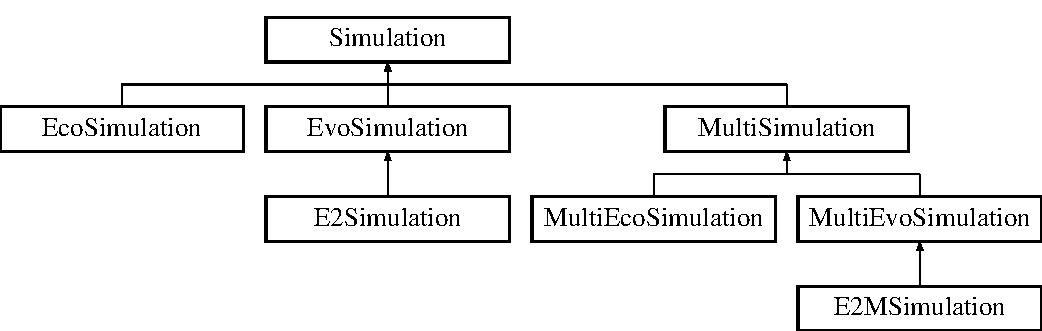
\includegraphics[height=4.000000cm]{classSimulation}
\end{center}
\end{figure}
\subsection*{Public Member Functions}
\begin{DoxyCompactItemize}
\item 
\hypertarget{classSimulation_ae902fd16a0f0c24d3b49c96cead9fcf9}{}\label{classSimulation_ae902fd16a0f0c24d3b49c96cead9fcf9} 
{\bfseries Simulation} (vector$<$ \hyperlink{classEnvironment}{Environment} $>$ \+\_\+env)
\item 
\hypertarget{classSimulation_a44dc929698224fbf195b9d9936fae82a}{}\label{classSimulation_a44dc929698224fbf195b9d9936fae82a} 
bool {\bfseries get\+Complete\+Start} ()
\item 
\hypertarget{classSimulation_adca9200350aad6630085d6f50ef910f3}{}\label{classSimulation_adca9200350aad6630085d6f50ef910f3} 
void {\bfseries set\+Complete\+Start} (bool new\+Val)
\item 
\hypertarget{classSimulation_a31e406c0ad5849a8e6496393ccbb3483}{}\label{classSimulation_a31e406c0ad5849a8e6496393ccbb3483} 
bool {\bfseries get\+Complete\+End} ()
\item 
\hypertarget{classSimulation_a0e8a32be7804eca80992fa6d1d27b0be}{}\label{classSimulation_a0e8a32be7804eca80992fa6d1d27b0be} 
void {\bfseries set\+Complete\+End} (bool new\+Val)
\item 
\hypertarget{classSimulation_a0cf743fa59385016d9e699fb0093317c}{}\label{classSimulation_a0cf743fa59385016d9e699fb0093317c} 
int {\bfseries get\+Num\+Steps} ()
\item 
\hypertarget{classSimulation_a68c66b40439322e4bda57eaa11386ce6}{}\label{classSimulation_a68c66b40439322e4bda57eaa11386ce6} 
void {\bfseries set\+Num\+Steps} (int new\+Val)
\item 
\hypertarget{classSimulation_a57f25582cd263d9739e9d72e75832a67}{}\label{classSimulation_a57f25582cd263d9739e9d72e75832a67} 
int {\bfseries get\+Save\+Div} ()
\item 
\hypertarget{classSimulation_a5346ad2601beff7e3918e25dd667ab4b}{}\label{classSimulation_a5346ad2601beff7e3918e25dd667ab4b} 
void {\bfseries set\+Save\+Div} (int new\+Val)
\item 
\hypertarget{classSimulation_a0110a1fad0e2390ea90fa387fe09cbdc}{}\label{classSimulation_a0110a1fad0e2390ea90fa387fe09cbdc} 
vector$<$ \hyperlink{classEnvironment}{Environment} $>$ $\ast$ {\bfseries get\+Envs} ()
\item 
\hypertarget{classSimulation_a8223c6354f021efcb667815fbd0682c0}{}\label{classSimulation_a8223c6354f021efcb667815fbd0682c0} 
void {\bfseries add\+Env} (\hyperlink{classEnvironment}{Environment} new\+Val)
\item 
virtual int \hyperlink{classSimulation_a7eb16da89581b496d33b77efbb63b9cd}{run\+Sim} (int run\+Number)
\begin{DoxyCompactList}\small\item\em Method that runs the main loop of the simulation. \end{DoxyCompactList}\end{DoxyCompactItemize}
\subsection*{Protected Attributes}
\begin{DoxyCompactItemize}
\item 
int \hyperlink{classSimulation_a999ce13c1a3d4dca2bf92e346d8b709f}{num\+Steps}
\item 
int \hyperlink{classSimulation_ae8f095e92da49a648954416b351e27c8}{save\+Div}
\item 
bool \hyperlink{classSimulation_a84cd73f44cff4fdbbb40fb98b49f8026}{complete\+Start} = false
\item 
bool \hyperlink{classSimulation_a17bcf189d0f10fa47e4b2dc4b53d4939}{complete\+End} = false
\item 
vector$<$ \hyperlink{classEnvironment}{Environment} $>$ \hyperlink{classSimulation_a29309017ca18043de245ef843b56c533}{envs}
\end{DoxyCompactItemize}


\subsection{Detailed Description}
Class containing all \hyperlink{classEnvironment}{Environment} objects, as well control-\/flow attributes for the simulation. 

The \hyperlink{classSimulation}{Simulation} class contains all \hyperlink{classEnvironment}{Environment} objects. It updates them each time\+Step, and is also in charge of deciding when to save what (for all save types). 

\subsection{Member Function Documentation}
\hypertarget{classSimulation_a7eb16da89581b496d33b77efbb63b9cd}{}\label{classSimulation_a7eb16da89581b496d33b77efbb63b9cd} 
\index{Simulation@{Simulation}!run\+Sim@{run\+Sim}}
\index{run\+Sim@{run\+Sim}!Simulation@{Simulation}}
\subsubsection{\texorpdfstring{run\+Sim()}{runSim()}}
{\footnotesize\ttfamily int Simulation\+::run\+Sim (\begin{DoxyParamCaption}\item[{int}]{run\+Number }\end{DoxyParamCaption})\hspace{0.3cm}{\ttfamily [virtual]}}



Method that runs the main loop of the simulation. 


\begin{DoxyParams}{Parameters}
{\em run\+Number} & ID of the current run of the simulation. \\
\hline
\end{DoxyParams}


Reimplemented in \hyperlink{classMultiSimulation_a235347d04fd0c7e1a2e35d7a39e77583}{Multi\+Simulation}, \hyperlink{classMultiEvoSimulation_a89c9806ac998c06230cdd41cc6a532bf}{Multi\+Evo\+Simulation}, \hyperlink{classE2MSimulation_aeac4e92c10f89a5c953ace5b1327d20b}{E2\+M\+Simulation}, \hyperlink{classEvoSimulation_aa43aa351dec24c638e56995a67a4f0f5}{Evo\+Simulation}, \hyperlink{classE2Simulation_a28028881fd443d2445b562512cb2169c}{E2\+Simulation}, \hyperlink{classMultiEcoSimulation_ad490e089c083d06d80c62af9e1564ac3}{Multi\+Eco\+Simulation}, and \hyperlink{classEcoSimulation_a72ec5e7dffb4231b2cb363b632788622}{Eco\+Simulation}.



\subsection{Member Data Documentation}
\hypertarget{classSimulation_a17bcf189d0f10fa47e4b2dc4b53d4939}{}\label{classSimulation_a17bcf189d0f10fa47e4b2dc4b53d4939} 
\index{Simulation@{Simulation}!complete\+End@{complete\+End}}
\index{complete\+End@{complete\+End}!Simulation@{Simulation}}
\subsubsection{\texorpdfstring{complete\+End}{completeEnd}}
{\footnotesize\ttfamily bool Simulation\+::complete\+End = false\hspace{0.3cm}{\ttfamily [protected]}}

Determines whether or not a complete save is made at the end of the simulation. \hypertarget{classSimulation_a84cd73f44cff4fdbbb40fb98b49f8026}{}\label{classSimulation_a84cd73f44cff4fdbbb40fb98b49f8026} 
\index{Simulation@{Simulation}!complete\+Start@{complete\+Start}}
\index{complete\+Start@{complete\+Start}!Simulation@{Simulation}}
\subsubsection{\texorpdfstring{complete\+Start}{completeStart}}
{\footnotesize\ttfamily bool Simulation\+::complete\+Start = false\hspace{0.3cm}{\ttfamily [protected]}}

Determines whether or not a complete save is made at the beginning of the simulation. \hypertarget{classSimulation_a29309017ca18043de245ef843b56c533}{}\label{classSimulation_a29309017ca18043de245ef843b56c533} 
\index{Simulation@{Simulation}!envs@{envs}}
\index{envs@{envs}!Simulation@{Simulation}}
\subsubsection{\texorpdfstring{envs}{envs}}
{\footnotesize\ttfamily vector$<$\hyperlink{classEnvironment}{Environment}$>$ Simulation\+::envs\hspace{0.3cm}{\ttfamily [protected]}}

List containing all environments of the simulation \hypertarget{classSimulation_a999ce13c1a3d4dca2bf92e346d8b709f}{}\label{classSimulation_a999ce13c1a3d4dca2bf92e346d8b709f} 
\index{Simulation@{Simulation}!num\+Steps@{num\+Steps}}
\index{num\+Steps@{num\+Steps}!Simulation@{Simulation}}
\subsubsection{\texorpdfstring{num\+Steps}{numSteps}}
{\footnotesize\ttfamily int Simulation\+::num\+Steps\hspace{0.3cm}{\ttfamily [protected]}}

Number of steps for which the simulation should be run \hypertarget{classSimulation_ae8f095e92da49a648954416b351e27c8}{}\label{classSimulation_ae8f095e92da49a648954416b351e27c8} 
\index{Simulation@{Simulation}!save\+Div@{save\+Div}}
\index{save\+Div@{save\+Div}!Simulation@{Simulation}}
\subsubsection{\texorpdfstring{save\+Div}{saveDiv}}
{\footnotesize\ttfamily int Simulation\+::save\+Div\hspace{0.3cm}{\ttfamily [protected]}}

Each how many steps densities are saved (in raw\+Save file) 

The documentation for this class was generated from the following files\+:\begin{DoxyCompactItemize}
\item 
\hyperlink{Simulation_8hpp}{Simulation.\+hpp}\item 
Simulation.\+cpp\end{DoxyCompactItemize}

\hypertarget{structsimValues}{}\section{sim\+Values Struct Reference}
\label{structsimValues}\index{sim\+Values@{sim\+Values}}


Structure containing all the values of the simulation we loaded.  




{\ttfamily \#include $<$reload\+Module.\+hpp$>$}

\subsection*{Public Attributes}
\begin{DoxyCompactItemize}
\item 
int \hyperlink{structsimValues_a409841bd1a747a200c99c86bfd11a78a}{old\+Spec}
\item 
int \hyperlink{structsimValues_ac7fbf812eba3e2b88996d1366131bf8e}{add\+Spec}
\item 
int \hyperlink{structsimValues_aeb4d9fe040a0ecb69669675753088a10}{tot\+Spec}
\item 
int \hyperlink{structsimValues_ae28b0e24d2b560548b1f4ba0eea035ee}{num\+Envs}
\item 
double \hyperlink{structsimValues_a0b3bdcfb8a911b35e71ab03aad776453}{env\+Const} = 0
\item 
vector$<$ int $>$ \hyperlink{structsimValues_a0c396a3dc37a1ecf668cbf0d6f52305f}{gen\+Times}
\item 
vector$<$ int $>$ \hyperlink{structsimValues_a658893629c5a789c447057da417e5096}{dens\+To\+Inds}
\item 
vector$<$ int $>$ \hyperlink{structsimValues_afe2312ca2bca46eac7a108d1aa9c88f0}{I\+Ds}
\item 
vector$<$ double $>$ \hyperlink{structsimValues_aa7977c641471b71ca3f88d98e2b01831}{alphas}
\item 
vector$<$ double $>$ \hyperlink{structsimValues_ab7b209f99b228a55680d64fc964b0d34}{betas}
\item 
vector$<$ double $>$ \hyperlink{structsimValues_a08f1c4e0b6042043876d9d2d2699a922}{ccs}
\item 
vector$<$ double $>$ \hyperlink{structsimValues_a14ed3f6bacb44ceb58b7929e90fe0516}{densities}
\item 
vector$<$ double $>$ \hyperlink{structsimValues_ab00d0541616bb1d309639954b90b3e1d}{optimums}
\item 
vector$<$ double $>$ \hyperlink{structsimValues_a8b045e15d8493873f87bbfb99cc6c10d}{opt\+Range}
\item 
vector$<$ vector$<$ double $>$ $>$ \hyperlink{structsimValues_afacf91cde42df4983ac4640c6fe78470}{interactions}
\item 
vector$<$ vector$<$ double $>$ $>$ \hyperlink{structsimValues_a5c4fa1fbabac24649729c3692bd2a59f}{evo\+Ranges}
\item 
vector$<$ vector$<$ vector$<$ vector$<$ double $>$ $>$ $>$ $>$ \hyperlink{structsimValues_a6745659920f5fb456202f8c84cb75a46}{routes}
\end{DoxyCompactItemize}


\subsection{Detailed Description}
Structure containing all the values of the simulation we loaded. 

This structure will be populated with the values from the complete save file used to reload the simulation. There will be one of these structures filled for each environment of the old simulation. 

\subsection{Member Data Documentation}
\hypertarget{structsimValues_ac7fbf812eba3e2b88996d1366131bf8e}{}\label{structsimValues_ac7fbf812eba3e2b88996d1366131bf8e} 
\index{sim\+Values@{sim\+Values}!add\+Spec@{add\+Spec}}
\index{add\+Spec@{add\+Spec}!sim\+Values@{sim\+Values}}
\subsubsection{\texorpdfstring{add\+Spec}{addSpec}}
{\footnotesize\ttfamily int sim\+Values\+::add\+Spec}

Number of \hyperlink{classSpecies}{Species} to add in the new simulation \hypertarget{structsimValues_aa7977c641471b71ca3f88d98e2b01831}{}\label{structsimValues_aa7977c641471b71ca3f88d98e2b01831} 
\index{sim\+Values@{sim\+Values}!alphas@{alphas}}
\index{alphas@{alphas}!sim\+Values@{sim\+Values}}
\subsubsection{\texorpdfstring{alphas}{alphas}}
{\footnotesize\ttfamily vector$<$double$>$ sim\+Values\+::alphas}

Alphas of (live) \hyperlink{classSpecies}{Species} in old simulation \hypertarget{structsimValues_ab7b209f99b228a55680d64fc964b0d34}{}\label{structsimValues_ab7b209f99b228a55680d64fc964b0d34} 
\index{sim\+Values@{sim\+Values}!betas@{betas}}
\index{betas@{betas}!sim\+Values@{sim\+Values}}
\subsubsection{\texorpdfstring{betas}{betas}}
{\footnotesize\ttfamily vector$<$double$>$ sim\+Values\+::betas}

Betas of (live) \hyperlink{classSpecies}{Species} in old simulation \hypertarget{structsimValues_a08f1c4e0b6042043876d9d2d2699a922}{}\label{structsimValues_a08f1c4e0b6042043876d9d2d2699a922} 
\index{sim\+Values@{sim\+Values}!ccs@{ccs}}
\index{ccs@{ccs}!sim\+Values@{sim\+Values}}
\subsubsection{\texorpdfstring{ccs}{ccs}}
{\footnotesize\ttfamily vector$<$double$>$ sim\+Values\+::ccs}

Carrying capacity (cc) of (live) \hyperlink{classSpecies}{Species} in old simulation \hypertarget{structsimValues_a14ed3f6bacb44ceb58b7929e90fe0516}{}\label{structsimValues_a14ed3f6bacb44ceb58b7929e90fe0516} 
\index{sim\+Values@{sim\+Values}!densities@{densities}}
\index{densities@{densities}!sim\+Values@{sim\+Values}}
\subsubsection{\texorpdfstring{densities}{densities}}
{\footnotesize\ttfamily vector$<$double$>$ sim\+Values\+::densities}

Densities of (live) \hyperlink{classSpecies}{Species} in old simulation \hypertarget{structsimValues_a658893629c5a789c447057da417e5096}{}\label{structsimValues_a658893629c5a789c447057da417e5096} 
\index{sim\+Values@{sim\+Values}!dens\+To\+Inds@{dens\+To\+Inds}}
\index{dens\+To\+Inds@{dens\+To\+Inds}!sim\+Values@{sim\+Values}}
\subsubsection{\texorpdfstring{dens\+To\+Inds}{densToInds}}
{\footnotesize\ttfamily vector$<$int$>$ sim\+Values\+::dens\+To\+Inds}

Number of individuals per units of density for each \hyperlink{classSpecies}{Species} \hypertarget{structsimValues_a0b3bdcfb8a911b35e71ab03aad776453}{}\label{structsimValues_a0b3bdcfb8a911b35e71ab03aad776453} 
\index{sim\+Values@{sim\+Values}!env\+Const@{env\+Const}}
\index{env\+Const@{env\+Const}!sim\+Values@{sim\+Values}}
\subsubsection{\texorpdfstring{env\+Const}{envConst}}
{\footnotesize\ttfamily double sim\+Values\+::env\+Const = 0}

Value of the environmental constant \hypertarget{structsimValues_a5c4fa1fbabac24649729c3692bd2a59f}{}\label{structsimValues_a5c4fa1fbabac24649729c3692bd2a59f} 
\index{sim\+Values@{sim\+Values}!evo\+Ranges@{evo\+Ranges}}
\index{evo\+Ranges@{evo\+Ranges}!sim\+Values@{sim\+Values}}
\subsubsection{\texorpdfstring{evo\+Ranges}{evoRanges}}
{\footnotesize\ttfamily vector$<$vector $<$double$>$ $>$ sim\+Values\+::evo\+Ranges}

Range of evolution of interaction values of (live) \hyperlink{classSpecies}{Species} in old simulation \hypertarget{structsimValues_a0c396a3dc37a1ecf668cbf0d6f52305f}{}\label{structsimValues_a0c396a3dc37a1ecf668cbf0d6f52305f} 
\index{sim\+Values@{sim\+Values}!gen\+Times@{gen\+Times}}
\index{gen\+Times@{gen\+Times}!sim\+Values@{sim\+Values}}
\subsubsection{\texorpdfstring{gen\+Times}{genTimes}}
{\footnotesize\ttfamily vector$<$int$>$ sim\+Values\+::gen\+Times}

Rates of evolution for each \hyperlink{classSpecies}{Species} \hypertarget{structsimValues_afe2312ca2bca46eac7a108d1aa9c88f0}{}\label{structsimValues_afe2312ca2bca46eac7a108d1aa9c88f0} 
\index{sim\+Values@{sim\+Values}!I\+Ds@{I\+Ds}}
\index{I\+Ds@{I\+Ds}!sim\+Values@{sim\+Values}}
\subsubsection{\texorpdfstring{I\+Ds}{IDs}}
{\footnotesize\ttfamily vector$<$int$>$ sim\+Values\+::\+I\+Ds}

I\+Ds of live \hyperlink{classSpecies}{Species} when the complete save was made \hypertarget{structsimValues_afacf91cde42df4983ac4640c6fe78470}{}\label{structsimValues_afacf91cde42df4983ac4640c6fe78470} 
\index{sim\+Values@{sim\+Values}!interactions@{interactions}}
\index{interactions@{interactions}!sim\+Values@{sim\+Values}}
\subsubsection{\texorpdfstring{interactions}{interactions}}
{\footnotesize\ttfamily vector$<$vector $<$double$>$ $>$ sim\+Values\+::interactions}

Interaction values of (live) \hyperlink{classSpecies}{Species} in old simulation \hypertarget{structsimValues_ae28b0e24d2b560548b1f4ba0eea035ee}{}\label{structsimValues_ae28b0e24d2b560548b1f4ba0eea035ee} 
\index{sim\+Values@{sim\+Values}!num\+Envs@{num\+Envs}}
\index{num\+Envs@{num\+Envs}!sim\+Values@{sim\+Values}}
\subsubsection{\texorpdfstring{num\+Envs}{numEnvs}}
{\footnotesize\ttfamily int sim\+Values\+::num\+Envs}

Numnber of environment in the simulaiton (same for old and new) \hypertarget{structsimValues_a409841bd1a747a200c99c86bfd11a78a}{}\label{structsimValues_a409841bd1a747a200c99c86bfd11a78a} 
\index{sim\+Values@{sim\+Values}!old\+Spec@{old\+Spec}}
\index{old\+Spec@{old\+Spec}!sim\+Values@{sim\+Values}}
\subsubsection{\texorpdfstring{old\+Spec}{oldSpec}}
{\footnotesize\ttfamily int sim\+Values\+::old\+Spec}

Number of \hyperlink{classSpecies}{Species} that were alive at the end of the old simulation \hypertarget{structsimValues_ab00d0541616bb1d309639954b90b3e1d}{}\label{structsimValues_ab00d0541616bb1d309639954b90b3e1d} 
\index{sim\+Values@{sim\+Values}!optimums@{optimums}}
\index{optimums@{optimums}!sim\+Values@{sim\+Values}}
\subsubsection{\texorpdfstring{optimums}{optimums}}
{\footnotesize\ttfamily vector$<$double$>$ sim\+Values\+::optimums}

Optimumss of (live) \hyperlink{classSpecies}{Species} in old simulation \hypertarget{structsimValues_a8b045e15d8493873f87bbfb99cc6c10d}{}\label{structsimValues_a8b045e15d8493873f87bbfb99cc6c10d} 
\index{sim\+Values@{sim\+Values}!opt\+Range@{opt\+Range}}
\index{opt\+Range@{opt\+Range}!sim\+Values@{sim\+Values}}
\subsubsection{\texorpdfstring{opt\+Range}{optRange}}
{\footnotesize\ttfamily vector$<$double$>$ sim\+Values\+::opt\+Range}

Range of optimum evolution of (live) \hyperlink{classSpecies}{Species} in old simulation \hypertarget{structsimValues_a6745659920f5fb456202f8c84cb75a46}{}\label{structsimValues_a6745659920f5fb456202f8c84cb75a46} 
\index{sim\+Values@{sim\+Values}!routes@{routes}}
\index{routes@{routes}!sim\+Values@{sim\+Values}}
\subsubsection{\texorpdfstring{routes}{routes}}
{\footnotesize\ttfamily vector$<$vector$<$vector$<$vector$<$double$>$ $>$ $>$ $>$ sim\+Values\+::routes}

Migration routes of (live) \hyperlink{classSpecies}{Species} in old simulation \hypertarget{structsimValues_aeb4d9fe040a0ecb69669675753088a10}{}\label{structsimValues_aeb4d9fe040a0ecb69669675753088a10} 
\index{sim\+Values@{sim\+Values}!tot\+Spec@{tot\+Spec}}
\index{tot\+Spec@{tot\+Spec}!sim\+Values@{sim\+Values}}
\subsubsection{\texorpdfstring{tot\+Spec}{totSpec}}
{\footnotesize\ttfamily int sim\+Values\+::tot\+Spec}

Total number of \hyperlink{classSpecies}{Species} in the new simulation 

The documentation for this struct was generated from the following file\+:\begin{DoxyCompactItemize}
\item 
\hyperlink{reloadModule_8hpp}{reload\+Module.\+hpp}\end{DoxyCompactItemize}

\hypertarget{classSpecies}{}\section{Species Class Reference}
\label{classSpecies}\index{Species@{Species}}


Class containing all parameters\&methods that define a species \& it\textquotesingle{}s interactions with other species/the environment.  




{\ttfamily \#include $<$Species.\+hpp$>$}

\subsection*{Public Member Functions}
\begin{DoxyCompactItemize}
\item 
\mbox{\Hypertarget{classSpecies_a385a49104d5d6d6aee34a983e589832b}\label{classSpecies_a385a49104d5d6d6aee34a983e589832b}} 
{\bfseries Species} (int \+\_\+num\+Self, int \+\_\+num\+Total, int \+\_\+gen\+Time, int \+\_\+ind\+To\+Dens, double \+\_\+alpha, double \+\_\+beta, double \+\_\+dens, double \+\_\+cc, double \+\_\+opt, double \+\_\+opt\+Range, double $\ast$\+\_\+env\+Const, vector$<$ double $>$ \+\_\+interactions, vector$<$ double $>$ \+\_\+range, vector$<$ vector$<$ vector$<$ double $>$$>$$>$ \+\_\+migration\+Routes, unique\+\_\+ptr$<$ \hyperlink{classChange}{Change} $>$ \+\_\+change, unique\+\_\+ptr$<$ \hyperlink{classEvo}{Evo} $>$ \+\_\+evo)
\item 
\mbox{\Hypertarget{classSpecies_acdddfb4cb6f496fee642b7c58f39d3f1}\label{classSpecies_acdddfb4cb6f496fee642b7c58f39d3f1}} 
int {\bfseries get\+Num\+Self} ()
\item 
\mbox{\Hypertarget{classSpecies_a31566bcf2f8647e9498ee2fec28531fb}\label{classSpecies_a31566bcf2f8647e9498ee2fec28531fb}} 
int {\bfseries get\+Num\+Total} ()
\item 
\mbox{\Hypertarget{classSpecies_af15e54343492700ff8841c3563bd9a0c}\label{classSpecies_af15e54343492700ff8841c3563bd9a0c}} 
int {\bfseries get\+Gen\+Time} ()
\item 
\mbox{\Hypertarget{classSpecies_a9951ad56ce265722c633b461f00bbb66}\label{classSpecies_a9951ad56ce265722c633b461f00bbb66}} 
double {\bfseries get\+Alpha} ()
\item 
\mbox{\Hypertarget{classSpecies_ae7a743e1bd001b01d17384763cdfbdee}\label{classSpecies_ae7a743e1bd001b01d17384763cdfbdee}} 
double {\bfseries get\+Beta} ()
\item 
\mbox{\Hypertarget{classSpecies_acb9612a527b867219571604e06a9b96a}\label{classSpecies_acb9612a527b867219571604e06a9b96a}} 
double {\bfseries get\+Density} ()
\item 
\mbox{\Hypertarget{classSpecies_a638225fa251d88eb8fefe25575791df9}\label{classSpecies_a638225fa251d88eb8fefe25575791df9}} 
void {\bfseries set\+Density} (double new\+Val)
\item 
\mbox{\Hypertarget{classSpecies_a674fddbf5e26a31280c9d0a8e423af47}\label{classSpecies_a674fddbf5e26a31280c9d0a8e423af47}} 
double {\bfseries get\+Previous\+Density} ()
\item 
\mbox{\Hypertarget{classSpecies_a762477a6c0f86748638a8cb41c677c84}\label{classSpecies_a762477a6c0f86748638a8cb41c677c84}} 
void {\bfseries set\+Previous\+Density} (double new\+Val)
\item 
\mbox{\Hypertarget{classSpecies_abe2828fd01669eac6359b1fb30d02f96}\label{classSpecies_abe2828fd01669eac6359b1fb30d02f96}} 
double {\bfseries get\+Cc} ()
\item 
\mbox{\Hypertarget{classSpecies_a5f2ab7671a625cc25bbfee399b4a388a}\label{classSpecies_a5f2ab7671a625cc25bbfee399b4a388a}} 
double {\bfseries get\+Opt\+Range} ()
\item 
\mbox{\Hypertarget{classSpecies_aa7f142ce10d699c3e222aed1e9527153}\label{classSpecies_aa7f142ce10d699c3e222aed1e9527153}} 
int {\bfseries get\+Ind\+To\+Dens} ()
\item 
\mbox{\Hypertarget{classSpecies_a972f259afd0683125f29ab396afe7b90}\label{classSpecies_a972f259afd0683125f29ab396afe7b90}} 
vector$<$ double $>$ {\bfseries get\+Range} ()
\item 
\mbox{\Hypertarget{classSpecies_af1cfadceaecbb1c27134638d56a2da79}\label{classSpecies_af1cfadceaecbb1c27134638d56a2da79}} 
double $\ast$ {\bfseries get\+Env\+Const} ()
\item 
\mbox{\Hypertarget{classSpecies_a77083a8913e501f92abfdfdc0b376249}\label{classSpecies_a77083a8913e501f92abfdfdc0b376249}} 
double {\bfseries get\+Optimum} ()
\item 
\mbox{\Hypertarget{classSpecies_ad800e8f89d4ea0b68644d58ba4796d88}\label{classSpecies_ad800e8f89d4ea0b68644d58ba4796d88}} 
void {\bfseries set\+Optimum} (double new\+Val)
\item 
\mbox{\Hypertarget{classSpecies_a0f1fb546bb844fbeb9486888bddfd666}\label{classSpecies_a0f1fb546bb844fbeb9486888bddfd666}} 
vector$<$ double $>$ $\ast$ {\bfseries get\+Interactions} ()
\item 
\mbox{\Hypertarget{classSpecies_a13bd812c3a366cf4a3bf9bd3e1e4d3fa}\label{classSpecies_a13bd812c3a366cf4a3bf9bd3e1e4d3fa}} 
double {\bfseries get\+Interaction} (int index)
\item 
\mbox{\Hypertarget{classSpecies_a3cf0a84408e2e0e6981654dc4a9f4eeb}\label{classSpecies_a3cf0a84408e2e0e6981654dc4a9f4eeb}} 
void {\bfseries set\+Interactions} (vector$<$ double $>$ new\+Val)
\item 
\mbox{\Hypertarget{classSpecies_a2158c22a9098d6591c829fb54611fc03}\label{classSpecies_a2158c22a9098d6591c829fb54611fc03}} 
void {\bfseries set\+Interaction} (int index, double new\+Val)
\item 
\mbox{\Hypertarget{classSpecies_ab219377e317d2c8d07a0a207f52cf3f4}\label{classSpecies_ab219377e317d2c8d07a0a207f52cf3f4}} 
void {\bfseries delete\+Interaction} (int index)
\item 
\mbox{\Hypertarget{classSpecies_a3eeef473f91fe468ffd4d76964bb5f6f}\label{classSpecies_a3eeef473f91fe468ffd4d76964bb5f6f}} 
double {\bfseries get\+One\+Range} (int index)
\item 
vector$<$ double $>$ \hyperlink{classSpecies_a306aaa396cc99e223d46a577b14e1faf}{get\+Migration} (int env\+Num, int num\+Envs)
\begin{DoxyCompactList}\small\item\em Index of return value is the ID of environment, value is the size of the migration to that environment. \end{DoxyCompactList}\item 
\mbox{\Hypertarget{classSpecies_a43a78cb3d46d2c02669ca80c9d0ede7b}\label{classSpecies_a43a78cb3d46d2c02669ca80c9d0ede7b}} 
vector$<$ vector$<$ double $>$ $>$ {\bfseries get\+Routes\+One\+Env} (int env\+Num)
\item 
\mbox{\Hypertarget{classSpecies_a9a0c31d84cac35b7525b38919b8ad963}\label{classSpecies_a9a0c31d84cac35b7525b38919b8ad963}} 
vector$<$ vector$<$ vector$<$ double $>$ $>$ $>$ {\bfseries get\+All\+Routes} ()
\item 
\mbox{\Hypertarget{classSpecies_ac64bd2c5d579d513cca4502dddbdd484}\label{classSpecies_ac64bd2c5d579d513cca4502dddbdd484}} 
void {\bfseries set\+All\+Routes} (vector$<$ vector$<$ vector$<$ double $>$$>$$>$ routes)
\item 
\mbox{\Hypertarget{classSpecies_a766219b52815e5f25206084de418385e}\label{classSpecies_a766219b52815e5f25206084de418385e}} 
double \hyperlink{classSpecies_a766219b52815e5f25206084de418385e}{get\+Change} (double delta, vector$<$ unique\+\_\+ptr$<$ \hyperlink{classSpecies}{Species} $>$$>$ $\ast$species\+List)
\begin{DoxyCompactList}\small\item\em Calls function of the \hyperlink{classChange}{Change} object with the required parameters to calculate species density change (density remains unchanged after call). \end{DoxyCompactList}\item 
\mbox{\Hypertarget{classSpecies_afce47f18aa0a770ddcb53dd985cf5758}\label{classSpecies_afce47f18aa0a770ddcb53dd985cf5758}} 
void \hyperlink{classSpecies_afce47f18aa0a770ddcb53dd985cf5758}{get\+Evo} (vector$<$ unique\+\_\+ptr$<$ \hyperlink{classSpecies}{Species} $>$$>$ $\ast$species\+List, int resolution)
\begin{DoxyCompactList}\small\item\em Calls function of the \hyperlink{classEvo}{Evo} object with the required parameters to calculate the change in interction values/optimums (interaction/optimum values changed after call). This method is only needed in simulations with evolution. \end{DoxyCompactList}\end{DoxyCompactItemize}
\subsection*{Protected Attributes}
\begin{DoxyCompactItemize}
\item 
int \hyperlink{classSpecies_a11e7aac3c4a85723e8a9d00d00452508}{num\+Self}
\item 
int \hyperlink{classSpecies_af13ccb1fc01cff22d7a47201c1002fbc}{num\+Total}
\item 
int \hyperlink{classSpecies_a17c9e5d56923d9800bd9b2cfacbcba8b}{gen\+Time}
\item 
int \hyperlink{classSpecies_a3a11f42cb341349dadb706fff06f301d}{ind\+To\+Dens}
\item 
double \hyperlink{classSpecies_a28a22a5a1eef97867bd6e5d7db2c0c6a}{alpha}
\item 
double \hyperlink{classSpecies_ae4f30dc0bf280e80601fc39a0150f8f2}{beta}
\item 
double \hyperlink{classSpecies_a2d5f0b6b799578963257416fa5ad0630}{density}
\item 
double \hyperlink{classSpecies_a46b0370ca3501bdcec53545df9f44cf4}{previous\+Density}
\item 
double \hyperlink{classSpecies_afbf0d05fd5e3904c1ce62833942ef935}{cc}
\item 
double \hyperlink{classSpecies_a234d375e63c9be61d756b7e70d7d9397}{optimum}
\item 
double \hyperlink{classSpecies_ab7103281892ef74944f3f10df5ecbe69}{opt\+Range}
\item 
double $\ast$const \hyperlink{classSpecies_a95c7dd87e88653b245d52400b4134b68}{env\+Const}
\item 
vector$<$ double $>$ \hyperlink{classSpecies_a2ea9ab3b36448426b237f40dd4a1a18d}{interactions}
\item 
vector$<$ double $>$ \hyperlink{classSpecies_af95c9259381c434919dd4e9041a65bc7}{range}
\item 
vector$<$ vector$<$ vector$<$ double $>$ $>$ $>$ \hyperlink{classSpecies_a732dd85466e7156e8e51c7b44ea00f24}{migration\+Routes}
\item 
unique\+\_\+ptr$<$ \hyperlink{classChange}{Change} $>$ \hyperlink{classSpecies_a6517dbf3b05112b50baadc9479856dda}{change}
\item 
unique\+\_\+ptr$<$ \hyperlink{classEvo}{Evo} $>$ \hyperlink{classSpecies_a25d6cad0391b8d98c986e17bcb5c2586}{evo}
\end{DoxyCompactItemize}


\subsection{Detailed Description}
Class containing all parameters\&methods that define a species \& it\textquotesingle{}s interactions with other species/the environment. 

The species class is the most important class of this program, since it contains all the information necessary to evolve the system over time. To simplify the use of polymorphism in conjunction with c++ vectors, species contain all attributes and methods needed for every type of simulation, which means that species used in basic simulations use more memory than strictly necessary. If you want to strip down the species definition to limit memory usage, adapting the \hyperlink{initializers_8hpp_a1a78967080f9ce44c5062094c6495078}{init\+Specs()} function in initializers.\+cpp is necessary, but the rest should work fine. 

\subsection{Member Function Documentation}
\mbox{\Hypertarget{classSpecies_a306aaa396cc99e223d46a577b14e1faf}\label{classSpecies_a306aaa396cc99e223d46a577b14e1faf}} 
\index{Species@{Species}!get\+Migration@{get\+Migration}}
\index{get\+Migration@{get\+Migration}!Species@{Species}}
\subsubsection{\texorpdfstring{get\+Migration()}{getMigration()}}
{\footnotesize\ttfamily vector$<$ double $>$ Species\+::get\+Migration (\begin{DoxyParamCaption}\item[{int}]{env\+Num,  }\item[{int}]{num\+Envs }\end{DoxyParamCaption})}



Index of return value is the ID of environment, value is the size of the migration to that environment. 

Calculates size of migrations of this species to each envrionment (up to but not including num\+Envs) from env\+Num. Total migration size can, depending on migration parameters, be bigger than species density (but species density won\textquotesingle{}t become negative as a result). Co-\/ordinated by get\+Migrants() in \hyperlink{classEnvironment}{Environment} class. 
\begin{DoxyParams}{Parameters}
{\em env\+Num} & ID of the environment in which the species resides \\
\hline
{\em num\+Envs} & Number of environments in the simulation in total \\
\hline
\end{DoxyParams}
\begin{DoxyNote}{Note}
This method is only called when there are multiple environments 
\end{DoxyNote}


\subsection{Field Documentation}
\mbox{\Hypertarget{classSpecies_a28a22a5a1eef97867bd6e5d7db2c0c6a}\label{classSpecies_a28a22a5a1eef97867bd6e5d7db2c0c6a}} 
\index{Species@{Species}!alpha@{alpha}}
\index{alpha@{alpha}!Species@{Species}}
\subsubsection{\texorpdfstring{alpha}{alpha}}
{\footnotesize\ttfamily double Species\+::alpha\hspace{0.3cm}{\ttfamily [protected]}}

\hyperlink{classSpecies}{Species} growth rate \mbox{\Hypertarget{classSpecies_ae4f30dc0bf280e80601fc39a0150f8f2}\label{classSpecies_ae4f30dc0bf280e80601fc39a0150f8f2}} 
\index{Species@{Species}!beta@{beta}}
\index{beta@{beta}!Species@{Species}}
\subsubsection{\texorpdfstring{beta}{beta}}
{\footnotesize\ttfamily double Species\+::beta\hspace{0.3cm}{\ttfamily [protected]}}

\hyperlink{classSpecies}{Species} mortality rate \mbox{\Hypertarget{classSpecies_afbf0d05fd5e3904c1ce62833942ef935}\label{classSpecies_afbf0d05fd5e3904c1ce62833942ef935}} 
\index{Species@{Species}!cc@{cc}}
\index{cc@{cc}!Species@{Species}}
\subsubsection{\texorpdfstring{cc}{cc}}
{\footnotesize\ttfamily double Species\+::cc\hspace{0.3cm}{\ttfamily [protected]}}

\hyperlink{classSpecies}{Species} carrying capacity (can be exceeded due to interactions with other species) \mbox{\Hypertarget{classSpecies_a6517dbf3b05112b50baadc9479856dda}\label{classSpecies_a6517dbf3b05112b50baadc9479856dda}} 
\index{Species@{Species}!change@{change}}
\index{change@{change}!Species@{Species}}
\subsubsection{\texorpdfstring{change}{change}}
{\footnotesize\ttfamily unique\+\_\+ptr$<$\hyperlink{classChange}{Change}$>$ Species\+::change\hspace{0.3cm}{\ttfamily [protected]}}

Points to class that defines the way in which density change from one step to the next is calculated (see class \hyperlink{classChange}{Change} and its children for details) \mbox{\Hypertarget{classSpecies_a2d5f0b6b799578963257416fa5ad0630}\label{classSpecies_a2d5f0b6b799578963257416fa5ad0630}} 
\index{Species@{Species}!density@{density}}
\index{density@{density}!Species@{Species}}
\subsubsection{\texorpdfstring{density}{density}}
{\footnotesize\ttfamily double Species\+::density\hspace{0.3cm}{\ttfamily [protected]}}

\hyperlink{classSpecies}{Species} density \mbox{\Hypertarget{classSpecies_a95c7dd87e88653b245d52400b4134b68}\label{classSpecies_a95c7dd87e88653b245d52400b4134b68}} 
\index{Species@{Species}!env\+Const@{env\+Const}}
\index{env\+Const@{env\+Const}!Species@{Species}}
\subsubsection{\texorpdfstring{env\+Const}{envConst}}
{\footnotesize\ttfamily double$\ast$ const Species\+::env\+Const\hspace{0.3cm}{\ttfamily [protected]}}

Points to the environmental constant of the environment (only needed in simulations with an environmental constant) \mbox{\Hypertarget{classSpecies_a25d6cad0391b8d98c986e17bcb5c2586}\label{classSpecies_a25d6cad0391b8d98c986e17bcb5c2586}} 
\index{Species@{Species}!evo@{evo}}
\index{evo@{evo}!Species@{Species}}
\subsubsection{\texorpdfstring{evo}{evo}}
{\footnotesize\ttfamily unique\+\_\+ptr$<$\hyperlink{classEvo}{Evo}$>$ Species\+::evo\hspace{0.3cm}{\ttfamily [protected]}}

Points to class that defines how evolution happens (only needed in simulations with evolution). See class \hyperlink{classEvo}{Evo} and its children for more details. \mbox{\Hypertarget{classSpecies_a17c9e5d56923d9800bd9b2cfacbcba8b}\label{classSpecies_a17c9e5d56923d9800bd9b2cfacbcba8b}} 
\index{Species@{Species}!gen\+Time@{gen\+Time}}
\index{gen\+Time@{gen\+Time}!Species@{Species}}
\subsubsection{\texorpdfstring{gen\+Time}{genTime}}
{\footnotesize\ttfamily int Species\+::gen\+Time\hspace{0.3cm}{\ttfamily [protected]}}

Each how many time\+Steps an evolution event occurs (only needed in simulations with evolution) \mbox{\Hypertarget{classSpecies_a3a11f42cb341349dadb706fff06f301d}\label{classSpecies_a3a11f42cb341349dadb706fff06f301d}} 
\index{Species@{Species}!ind\+To\+Dens@{ind\+To\+Dens}}
\index{ind\+To\+Dens@{ind\+To\+Dens}!Species@{Species}}
\subsubsection{\texorpdfstring{ind\+To\+Dens}{indToDens}}
{\footnotesize\ttfamily int Species\+::ind\+To\+Dens\hspace{0.3cm}{\ttfamily [protected]}}

How many individuals are generated per unit of density (only needed in simulations with evolution) \mbox{\Hypertarget{classSpecies_a2ea9ab3b36448426b237f40dd4a1a18d}\label{classSpecies_a2ea9ab3b36448426b237f40dd4a1a18d}} 
\index{Species@{Species}!interactions@{interactions}}
\index{interactions@{interactions}!Species@{Species}}
\subsubsection{\texorpdfstring{interactions}{interactions}}
{\footnotesize\ttfamily vector$<$double$>$ Species\+::interactions\hspace{0.3cm}{\ttfamily [protected]}}

Vector containing interaction values for all species, index = species ID \mbox{\Hypertarget{classSpecies_a732dd85466e7156e8e51c7b44ea00f24}\label{classSpecies_a732dd85466e7156e8e51c7b44ea00f24}} 
\index{Species@{Species}!migration\+Routes@{migration\+Routes}}
\index{migration\+Routes@{migration\+Routes}!Species@{Species}}
\subsubsection{\texorpdfstring{migration\+Routes}{migrationRoutes}}
{\footnotesize\ttfamily vector$<$vector$<$vector$<$double$>$ $>$ $>$ Species\+::migration\+Routes\hspace{0.3cm}{\ttfamily [protected]}}

Routes from each env to each other, containing migration probability (\mbox{[}env\mbox{]}\mbox{[}env\mbox{]}\mbox{[}0\mbox{]}) and size(\mbox{[}env\mbox{]}\mbox{[}env\mbox{]}\mbox{[}1\mbox{]}). Only needed in simulations with multiple environments. \mbox{\Hypertarget{classSpecies_a11e7aac3c4a85723e8a9d00d00452508}\label{classSpecies_a11e7aac3c4a85723e8a9d00d00452508}} 
\index{Species@{Species}!num\+Self@{num\+Self}}
\index{num\+Self@{num\+Self}!Species@{Species}}
\subsubsection{\texorpdfstring{num\+Self}{numSelf}}
{\footnotesize\ttfamily int Species\+::num\+Self\hspace{0.3cm}{\ttfamily [protected]}}

ID of species \mbox{\Hypertarget{classSpecies_af13ccb1fc01cff22d7a47201c1002fbc}\label{classSpecies_af13ccb1fc01cff22d7a47201c1002fbc}} 
\index{Species@{Species}!num\+Total@{num\+Total}}
\index{num\+Total@{num\+Total}!Species@{Species}}
\subsubsection{\texorpdfstring{num\+Total}{numTotal}}
{\footnotesize\ttfamily int Species\+::num\+Total\hspace{0.3cm}{\ttfamily [protected]}}

Total number of species (all envrionments) \mbox{\Hypertarget{classSpecies_a234d375e63c9be61d756b7e70d7d9397}\label{classSpecies_a234d375e63c9be61d756b7e70d7d9397}} 
\index{Species@{Species}!optimum@{optimum}}
\index{optimum@{optimum}!Species@{Species}}
\subsubsection{\texorpdfstring{optimum}{optimum}}
{\footnotesize\ttfamily double Species\+::optimum\hspace{0.3cm}{\ttfamily [protected]}}

Value of the environmental constant at which species thrives best (only needed in simulations with an environmental constant) \mbox{\Hypertarget{classSpecies_ab7103281892ef74944f3f10df5ecbe69}\label{classSpecies_ab7103281892ef74944f3f10df5ecbe69}} 
\index{Species@{Species}!opt\+Range@{opt\+Range}}
\index{opt\+Range@{opt\+Range}!Species@{Species}}
\subsubsection{\texorpdfstring{opt\+Range}{optRange}}
{\footnotesize\ttfamily double Species\+::opt\+Range\hspace{0.3cm}{\ttfamily [protected]}}

Sigma parameter for generating optimums in indivudals (only needed in simulations with both evolution and environmental constant) \mbox{\Hypertarget{classSpecies_a46b0370ca3501bdcec53545df9f44cf4}\label{classSpecies_a46b0370ca3501bdcec53545df9f44cf4}} 
\index{Species@{Species}!previous\+Density@{previous\+Density}}
\index{previous\+Density@{previous\+Density}!Species@{Species}}
\subsubsection{\texorpdfstring{previous\+Density}{previousDensity}}
{\footnotesize\ttfamily double Species\+::previous\+Density\hspace{0.3cm}{\ttfamily [protected]}}

\hyperlink{classSpecies}{Species} density in the previous time\+Step \mbox{\Hypertarget{classSpecies_af95c9259381c434919dd4e9041a65bc7}\label{classSpecies_af95c9259381c434919dd4e9041a65bc7}} 
\index{Species@{Species}!range@{range}}
\index{range@{range}!Species@{Species}}
\subsubsection{\texorpdfstring{range}{range}}
{\footnotesize\ttfamily vector$<$double$>$ Species\+::range\hspace{0.3cm}{\ttfamily [protected]}}

sigma parameter for generating interactions in individuals (only needed in simulations with evolution) 

The documentation for this class was generated from the following files\+:\begin{DoxyCompactItemize}
\item 
\hyperlink{Species_8hpp}{Species.\+hpp}\item 
Species.\+cpp\end{DoxyCompactItemize}

\hypertarget{classStdChange}{}\section{Std\+Change Class Reference}
\label{classStdChange}\index{Std\+Change@{Std\+Change}}


Class containing just one function, used to calculate change in species density.  




{\ttfamily \#include $<$Std\+Change.\+hpp$>$}

Inheritance diagram for Std\+Change\+:\begin{figure}[H]
\begin{center}
\leavevmode
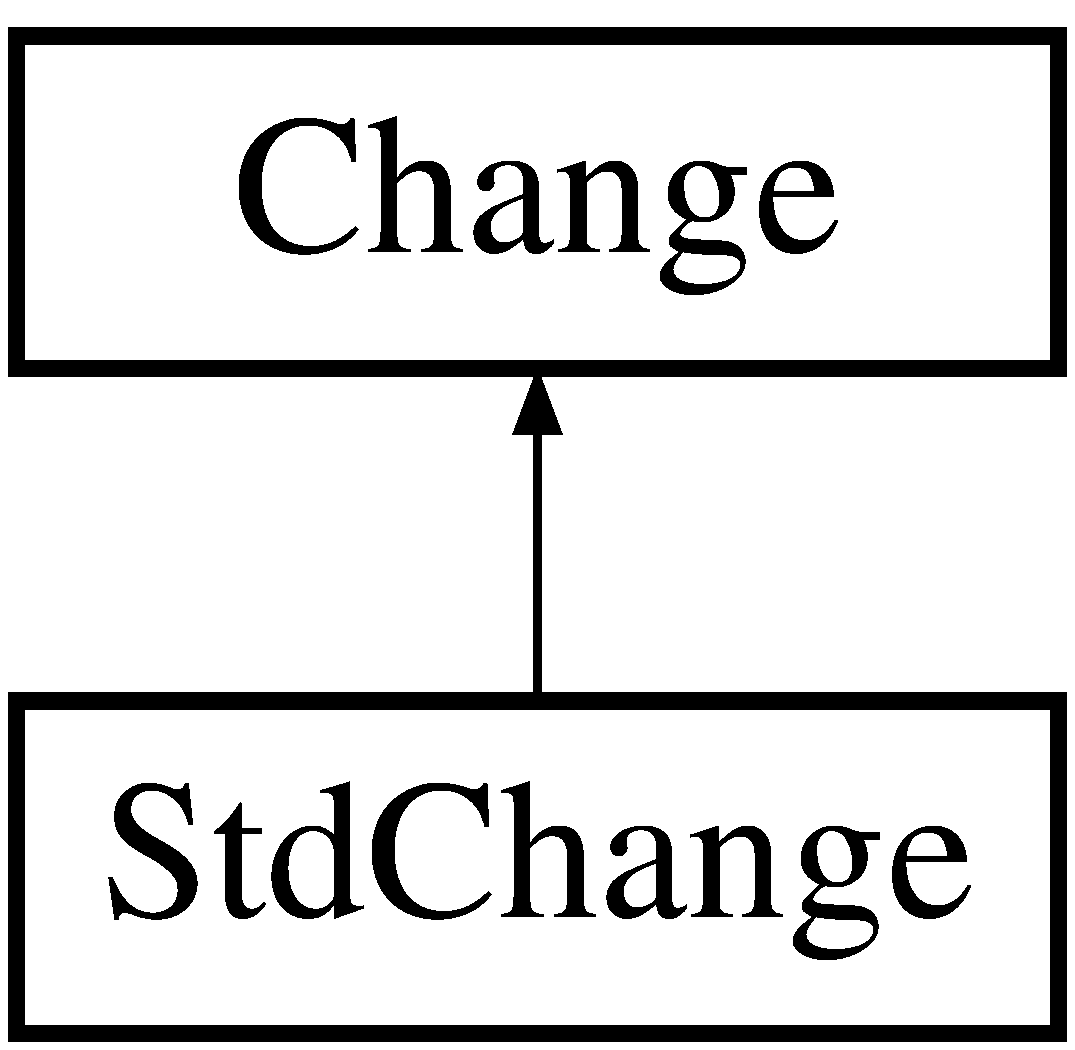
\includegraphics[height=2.000000cm]{classStdChange}
\end{center}
\end{figure}
\subsection*{Public Member Functions}
\begin{DoxyCompactItemize}
\item 
double \hyperlink{classStdChange_a25fd1a3828d026e902bae809278c6dbc}{get\+Change} (\hyperlink{classSpecies}{Species} $\ast$spec, double delta, vector$<$ unique\+\_\+ptr$<$ \hyperlink{classSpecies}{Species} $>$$>$ $\ast$species\+List)
\begin{DoxyCompactList}\small\item\em Method to calculate change in species density. \end{DoxyCompactList}\end{DoxyCompactItemize}


\subsection{Detailed Description}
Class containing just one function, used to calculate change in species density. 

The \hyperlink{classStdChange}{Std\+Change} class implements the inherited virtual method \hyperlink{classStdChange_a25fd1a3828d026e902bae809278c6dbc}{get\+Change()}, used to calculate change in species density. The implementation of \hyperlink{classStdChange}{Std\+Change} calculates change in species density as\+:

$\dot{x_i} = \delta * x_i * (\alpha + (1 - (cc/x_i)^2) + \beta + \sum_{j \neq i}^numTotal I_{ij} * x_j)$

where all parameters except $\delta$ are those of the species ( $x_i, x_j$ refer to density of species i and j, respectively). $\delta$ is owned by the environment. 

\subsection{Member Function Documentation}
\hypertarget{classStdChange_a25fd1a3828d026e902bae809278c6dbc}{}\label{classStdChange_a25fd1a3828d026e902bae809278c6dbc} 
\index{Std\+Change@{Std\+Change}!get\+Change@{get\+Change}}
\index{get\+Change@{get\+Change}!Std\+Change@{Std\+Change}}
\subsubsection{\texorpdfstring{get\+Change()}{getChange()}}
{\footnotesize\ttfamily double Std\+Change\+::get\+Change (\begin{DoxyParamCaption}\item[{\hyperlink{classSpecies}{Species} $\ast$}]{spec,  }\item[{double}]{delta,  }\item[{vector$<$ unique\+\_\+ptr$<$ \hyperlink{classSpecies}{Species} $>$$>$ $\ast$}]{species\+List }\end{DoxyParamCaption})\hspace{0.3cm}{\ttfamily [virtual]}}



Method to calculate change in species density. 

This method uses the explicit Euler scheme to resolve a Lotka-\/\+Volterra-\/like differential equation we use to calculate the evolution of the system. 
\begin{DoxyParams}{Parameters}
{\em spec} & \hyperlink{classSpecies}{Species} for which we will calculate change in density. \\
\hline
{\em delta} & size of step used in explicit Euler. \\
\hline
{\em species\+List} & List containing all (alive) species present in the environment. \\
\hline
\end{DoxyParams}


Implements \hyperlink{classChange_a59b9108e42a0aef74f735c1f82d4f014}{Change}.



The documentation for this class was generated from the following files\+:\begin{DoxyCompactItemize}
\item 
\hyperlink{StdChange_8hpp}{Std\+Change.\+hpp}\item 
Std\+Change.\+cpp\end{DoxyCompactItemize}

\hypertarget{classStdEvo}{}\section{Std\+Evo Class Reference}
\label{classStdEvo}\index{Std\+Evo@{Std\+Evo}}


Implementation of the \hyperlink{classEvo}{Evo} class that updates species interactions according to selection. \hyperlink{classSpecies}{Species} optimum is not affected.  




{\ttfamily \#include $<$Std\+Evo.\+hpp$>$}

Inheritance diagram for Std\+Evo\+:\begin{figure}[H]
\begin{center}
\leavevmode
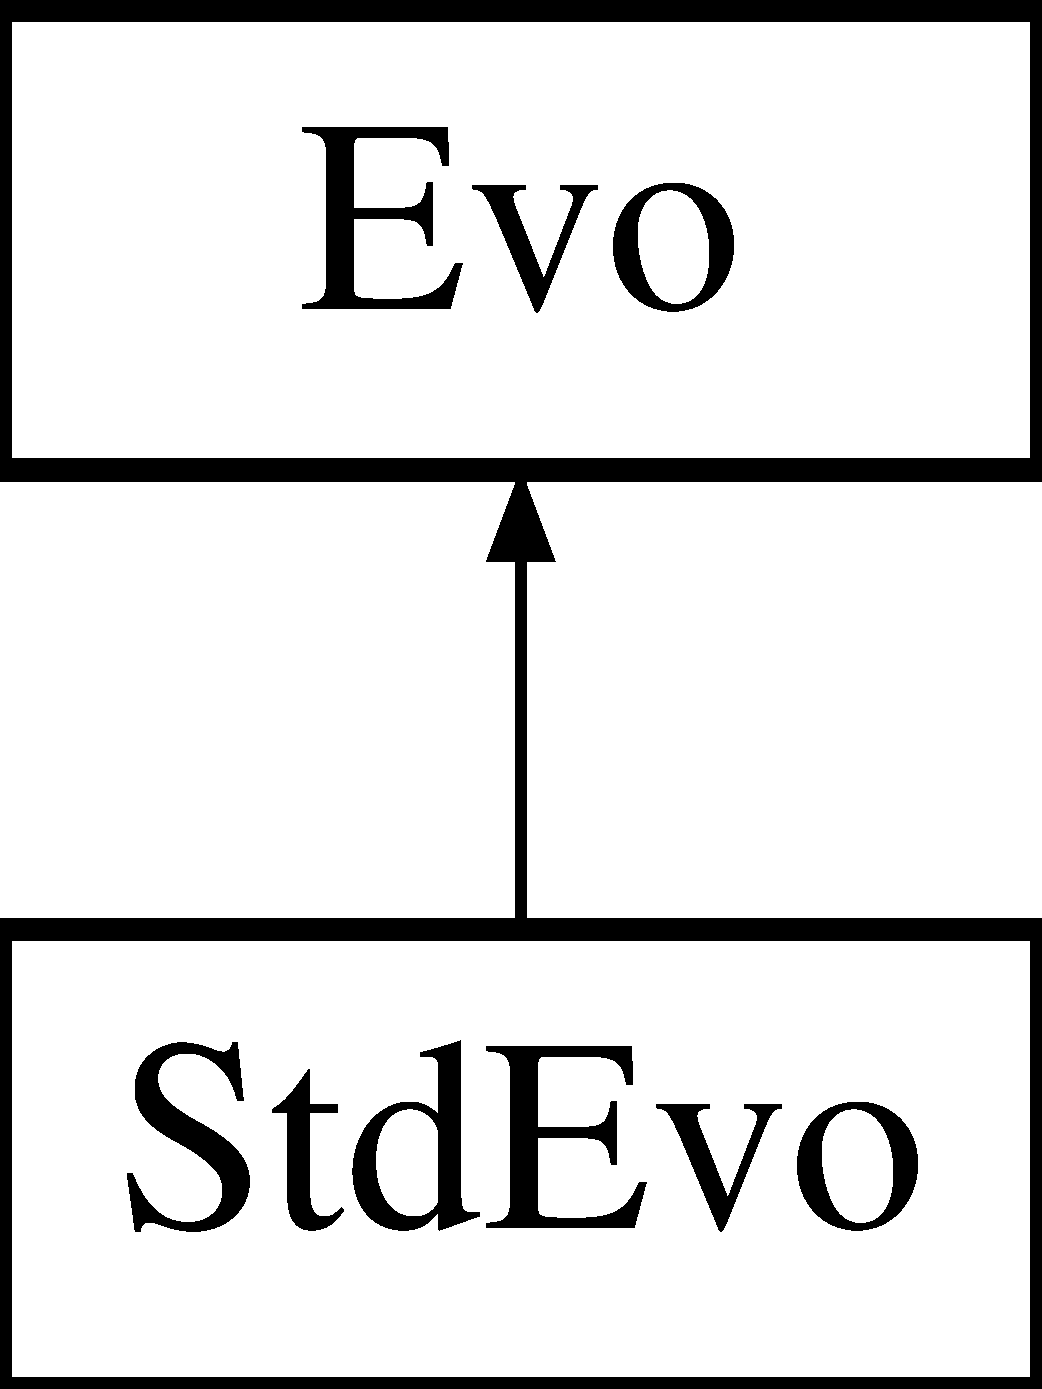
\includegraphics[height=2.000000cm]{classStdEvo}
\end{center}
\end{figure}
\subsection*{Public Member Functions}
\begin{DoxyCompactItemize}
\item 
void \hyperlink{classStdEvo_aa2b036f5e38510eca6cdbd60fc2bb23f}{get\+Evo} (vector$<$ unique\+\_\+ptr$<$ \hyperlink{classSpecies}{Species} $>$$>$ $\ast$species\+List, \hyperlink{classSpecies}{Species} $\ast$spec, int resolution)
\begin{DoxyCompactList}\small\item\em Controller method for updating species interactions/optimum. \end{DoxyCompactList}\item 
vector$<$ unique\+\_\+ptr$<$ \hyperlink{classIndividual}{Individual} $>$ $>$ \hyperlink{classStdEvo_a40bd3beb0e6f36baee1b40db279fd9b4}{get\+Inds} (vector$<$ unique\+\_\+ptr$<$ \hyperlink{classSpecies}{Species} $>$$>$ $\ast$species\+List, \hyperlink{classSpecies}{Species} $\ast$spec, int resolution)
\begin{DoxyCompactList}\small\item\em Method for creating individuals from species. \end{DoxyCompactList}\item 
vector$<$ int $>$ \hyperlink{classStdEvo_a6d4c64918a01dd00ad5185796b67e219}{run\+Selection} (vector$<$ unique\+\_\+ptr$<$ \hyperlink{classIndividual}{Individual} $>$$>$ $\ast$inds, vector$<$ unique\+\_\+ptr$<$ \hyperlink{classSpecies}{Species} $>$$>$ $\ast$species\+List)
\begin{DoxyCompactList}\small\item\em Method that selects surviving/reproducing individuals. \end{DoxyCompactList}\end{DoxyCompactItemize}
\subsection*{Additional Inherited Members}


\subsection{Detailed Description}
Implementation of the \hyperlink{classEvo}{Evo} class that updates species interactions according to selection. \hyperlink{classSpecies}{Species} optimum is not affected. 

\subsection{Member Function Documentation}
\hypertarget{classStdEvo_aa2b036f5e38510eca6cdbd60fc2bb23f}{}\label{classStdEvo_aa2b036f5e38510eca6cdbd60fc2bb23f} 
\index{Std\+Evo@{Std\+Evo}!get\+Evo@{get\+Evo}}
\index{get\+Evo@{get\+Evo}!Std\+Evo@{Std\+Evo}}
\subsubsection{\texorpdfstring{get\+Evo()}{getEvo()}}
{\footnotesize\ttfamily void Std\+Evo\+::get\+Evo (\begin{DoxyParamCaption}\item[{vector$<$ unique\+\_\+ptr$<$ \hyperlink{classSpecies}{Species} $>$$>$ $\ast$}]{species\+List,  }\item[{\hyperlink{classSpecies}{Species} $\ast$}]{spec,  }\item[{int}]{resolution }\end{DoxyParamCaption})\hspace{0.3cm}{\ttfamily [virtual]}}



Controller method for updating species interactions/optimum. 

Calls \hyperlink{classStdEvo_a40bd3beb0e6f36baee1b40db279fd9b4}{get\+Inds()} to get a list of individuals on which to call \hyperlink{classStdEvo_a6d4c64918a01dd00ad5185796b67e219}{run\+Selection()}. Then calculates the mean of all interaction values from selected individuals, and sets this as the new interaction values for the species.


\begin{DoxyParams}{Parameters}
{\em species\+List} & List containing all (alive) species present in the environment (used to calculate survival/reproduction probability of indivduals). \\
\hline
{\em spec} & \hyperlink{classSpecies}{Species} for which we will calculate evolutionary change (parameters are automatically updated during call). \\
\hline
{\em resolution} & How many discrete individuals are contained in one unit of density. \\
\hline
\end{DoxyParams}


Implements \hyperlink{classEvo_a8c5208c00d1ee2fe9bef41bdd7fe0ab7}{Evo}.

\hypertarget{classStdEvo_a40bd3beb0e6f36baee1b40db279fd9b4}{}\label{classStdEvo_a40bd3beb0e6f36baee1b40db279fd9b4} 
\index{Std\+Evo@{Std\+Evo}!get\+Inds@{get\+Inds}}
\index{get\+Inds@{get\+Inds}!Std\+Evo@{Std\+Evo}}
\subsubsection{\texorpdfstring{get\+Inds()}{getInds()}}
{\footnotesize\ttfamily vector$<$ unique\+\_\+ptr$<$ \hyperlink{classIndividual}{Individual} $>$ $>$ Std\+Evo\+::get\+Inds (\begin{DoxyParamCaption}\item[{vector$<$ unique\+\_\+ptr$<$ \hyperlink{classSpecies}{Species} $>$$>$ $\ast$}]{species\+List,  }\item[{\hyperlink{classSpecies}{Species} $\ast$}]{spec,  }\item[{int}]{resolution }\end{DoxyParamCaption})\hspace{0.3cm}{\ttfamily [virtual]}}



Method for creating individuals from species. 

This method divides a species with continous density into a discrete number of individuals {\ttfamily num\+Inds = round(species.\+density) $\ast$ resolution$<$$>$. Interaction values for each individual are generated from a gaussian distribution $\mathcal{N}(\mu , \sigma^2)$ where $\mu$ is species interaction value, and $\sigma^2$ is evolution range for that interaction.}

{\ttfamily 
\begin{DoxyParams}{Parameters}
{\em species\+List} & List containing all (alive) species present in the environment (used to calculate survival/reproduction probability of indivduals). \\
\hline
{\em spec} & \hyperlink{classSpecies}{Species} from which we will generate individuals. \\
\hline
{\em resolution} & How many discrete individuals are contained in one unit of density. \\
\hline
\end{DoxyParams}
}

Implements \hyperlink{classEvo_a88b5e0b1053cf1b4b473a08e2f03db92}{Evo}.

\hypertarget{classStdEvo_a6d4c64918a01dd00ad5185796b67e219}{}\label{classStdEvo_a6d4c64918a01dd00ad5185796b67e219} 
\index{Std\+Evo@{Std\+Evo}!run\+Selection@{run\+Selection}}
\index{run\+Selection@{run\+Selection}!Std\+Evo@{Std\+Evo}}
\subsubsection{\texorpdfstring{run\+Selection()}{runSelection()}}
{\footnotesize\ttfamily vector$<$ int $>$ Std\+Evo\+::run\+Selection (\begin{DoxyParamCaption}\item[{vector$<$ unique\+\_\+ptr$<$ \hyperlink{classIndividual}{Individual} $>$$>$ $\ast$}]{inds,  }\item[{vector$<$ unique\+\_\+ptr$<$ \hyperlink{classSpecies}{Species} $>$$>$ $\ast$}]{species\+List }\end{DoxyParamCaption})\hspace{0.3cm}{\ttfamily [virtual]}}



Method that selects surviving/reproducing individuals. 

This method calculates survival/reproduction probability for each individual (detailed in the \hyperlink{classIndividual}{Individual} class), and returns a list indicating how many copies of each individual will be in the next generation (either 2 or 0).


\begin{DoxyParams}{Parameters}
{\em inds} & List containing all individuals that were generated from evolving species. \\
\hline
{\em species\+List} & List containing all (alive) species present in the environment (used to calculate survival/reproduction probability of indivduals). \\
\hline
\end{DoxyParams}


Implements \hyperlink{classEvo_a10ff4eefe3967ff5cf5f820890c18079}{Evo}.



The documentation for this class was generated from the following files\+:\begin{DoxyCompactItemize}
\item 
\hyperlink{StdEvo_8hpp}{Std\+Evo.\+hpp}\item 
Std\+Evo.\+cpp\end{DoxyCompactItemize}

\hypertarget{classStdMultiNextGen}{}\section{Std\+Multi\+Next\+Gen Class Reference}
\label{classStdMultiNextGen}\index{Std\+Multi\+Next\+Gen@{Std\+Multi\+Next\+Gen}}


Class containing a single method, used to control transition from one step to the next, and update Species/\+Environemnt attributes.  




{\ttfamily \#include $<$Std\+Multi\+Next\+Gen.\+hpp$>$}

Inheritance diagram for Std\+Multi\+Next\+Gen\+:\begin{figure}[H]
\begin{center}
\leavevmode
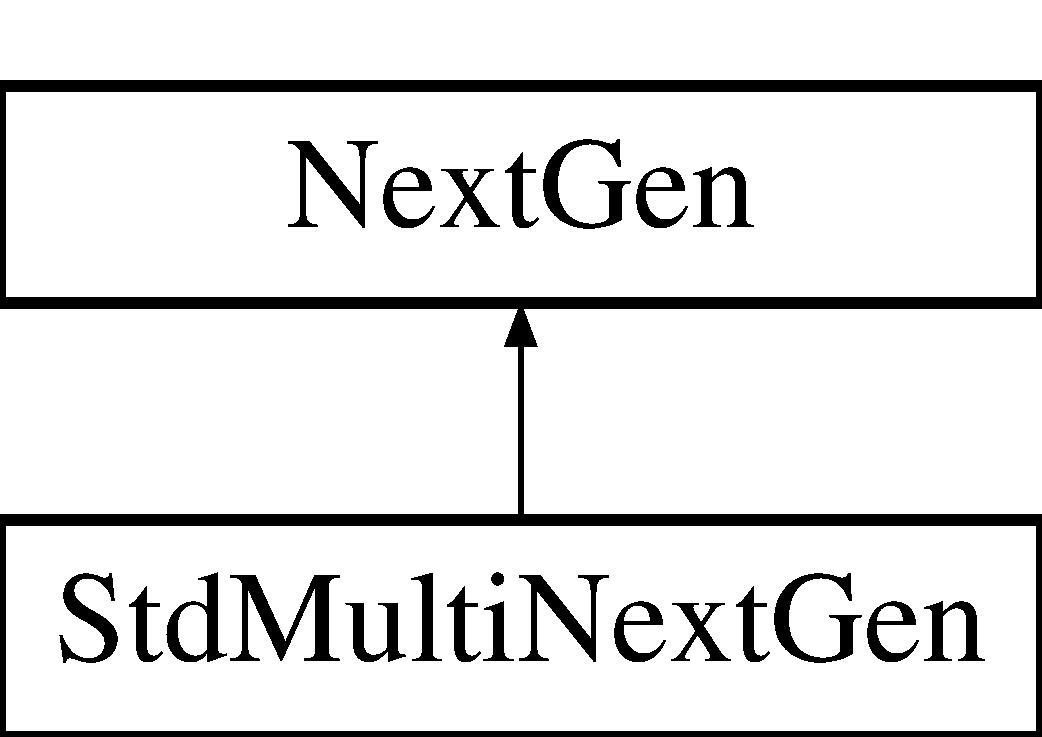
\includegraphics[height=2.000000cm]{classStdMultiNextGen}
\end{center}
\end{figure}
\subsection*{Public Member Functions}
\begin{DoxyCompactItemize}
\item 
void \hyperlink{classStdMultiNextGen_a4e3a48cdc731da26abe8b1f32cdbf962}{get\+Next\+Gen} (int step\+Num, std\+::vector$<$ std\+::unique\+\_\+ptr$<$ \hyperlink{classSpecies}{Species} $>$$>$ $\ast$species\+List, \hyperlink{classEnvironment}{Environment} $\ast$env)
\begin{DoxyCompactList}\small\item\em Method used to update \hyperlink{classSpecies}{Species} density at each timestep. \end{DoxyCompactList}\end{DoxyCompactItemize}


\subsection{Detailed Description}
Class containing a single method, used to control transition from one step to the next, and update Species/\+Environemnt attributes. 

\subsection{Member Function Documentation}
\mbox{\Hypertarget{classStdMultiNextGen_a4e3a48cdc731da26abe8b1f32cdbf962}\label{classStdMultiNextGen_a4e3a48cdc731da26abe8b1f32cdbf962}} 
\index{Std\+Multi\+Next\+Gen@{Std\+Multi\+Next\+Gen}!get\+Next\+Gen@{get\+Next\+Gen}}
\index{get\+Next\+Gen@{get\+Next\+Gen}!Std\+Multi\+Next\+Gen@{Std\+Multi\+Next\+Gen}}
\subsubsection{\texorpdfstring{get\+Next\+Gen()}{getNextGen()}}
{\footnotesize\ttfamily void Std\+Multi\+Next\+Gen\+::get\+Next\+Gen (\begin{DoxyParamCaption}\item[{int}]{step\+Num,  }\item[{std\+::vector$<$ std\+::unique\+\_\+ptr$<$ \hyperlink{classSpecies}{Species} $>$$>$ $\ast$}]{species\+List,  }\item[{\hyperlink{classEnvironment}{Environment} $\ast$}]{env }\end{DoxyParamCaption})\hspace{0.3cm}{\ttfamily [virtual]}}



Method used to update \hyperlink{classSpecies}{Species} density at each timestep. 

This method works exactly like the one in \hyperlink{classStdNextGen}{Std\+Next\+Gen}, except that species with {\ttfamily density == 0} are not moved to env.\+dead\+Species, to avoid having to recreate them if a population from said species migrates into environment from somewhere. If migration probability is very low for all species, it might be worth to delete/introduce them each time, since this might take less time than the increased loop time caused by a higher number of species (I\textquotesingle{}d say it depends on the simulation parameters, but I haven\textquotesingle{}t done any performance tests to compare the two methods).


\begin{DoxyParams}{Parameters}
{\em step\+Num} & Values of the current step \\
\hline
{\em species\+List} & List containing all \hyperlink{classSpecies}{Species} of the environment \\
\hline
{\em env} & Pointer to current environment \\
\hline
\end{DoxyParams}


Implements \hyperlink{classNextGen_aa70da77e0ac03da1bd5414c5e3fd70c0}{Next\+Gen}.



The documentation for this class was generated from the following files\+:\begin{DoxyCompactItemize}
\item 
\hyperlink{StdMultiNextGen_8hpp}{Std\+Multi\+Next\+Gen.\+hpp}\item 
Std\+Multi\+Next\+Gen.\+cpp\end{DoxyCompactItemize}

\hypertarget{classStdNextGen}{}\section{Std\+Next\+Gen Class Reference}
\label{classStdNextGen}\index{Std\+Next\+Gen@{Std\+Next\+Gen}}


Class containing a single method, used to control transition from one step to the next, and update Species/\+Environemnt attributes.  




{\ttfamily \#include $<$Std\+Next\+Gen.\+hpp$>$}

Inheritance diagram for Std\+Next\+Gen\+:\begin{figure}[H]
\begin{center}
\leavevmode
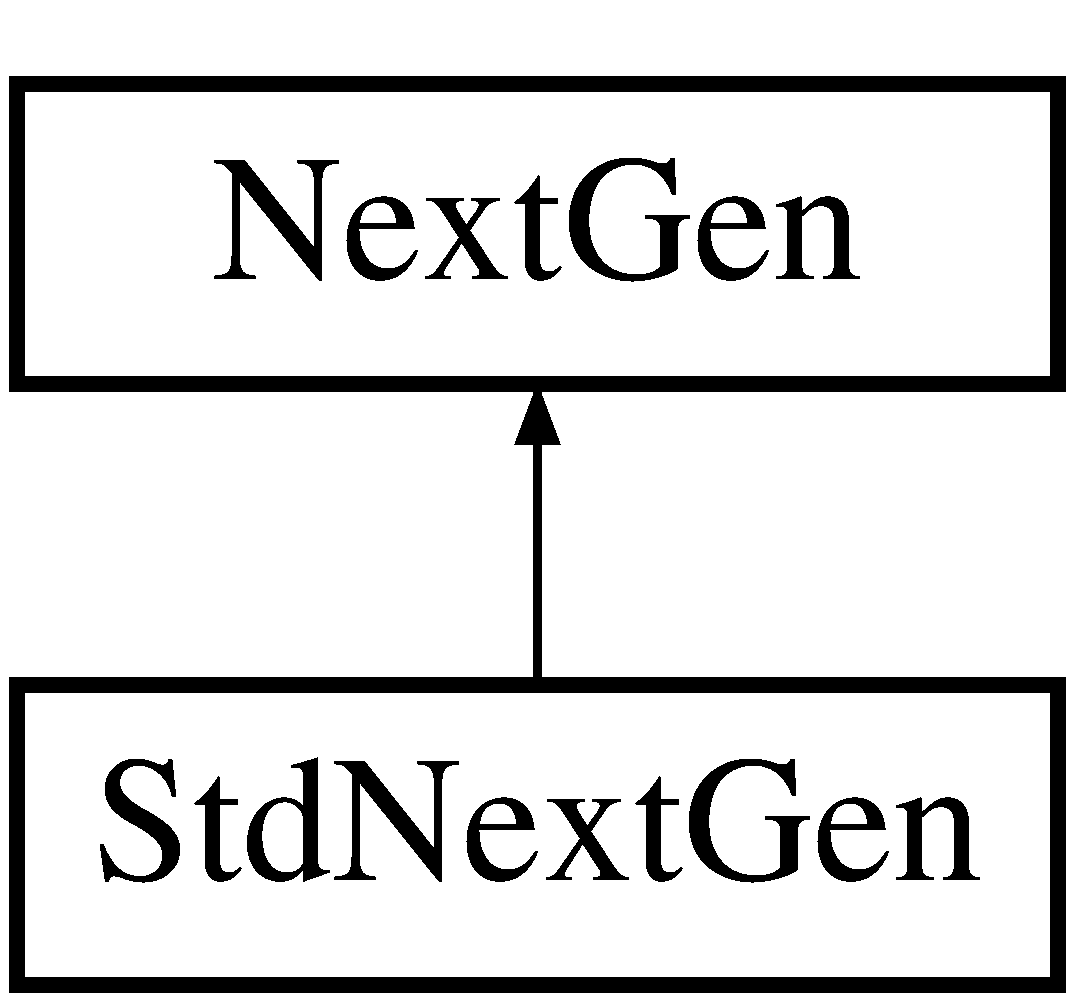
\includegraphics[height=2.000000cm]{classStdNextGen}
\end{center}
\end{figure}
\subsection*{Public Member Functions}
\begin{DoxyCompactItemize}
\item 
void \hyperlink{classStdNextGen_a2253fef9e33f6fe5f2e84f4dc89cfcd2}{get\+Next\+Gen} (int step\+Num, std\+::vector$<$ std\+::unique\+\_\+ptr$<$ \hyperlink{classSpecies}{Species} $>$$>$ $\ast$species\+List, \hyperlink{classEnvironment}{Environment} $\ast$env)
\begin{DoxyCompactList}\small\item\em Method used to update \hyperlink{classSpecies}{Species} density at each timestep. \end{DoxyCompactList}\end{DoxyCompactItemize}


\subsection{Detailed Description}
Class containing a single method, used to control transition from one step to the next, and update Species/\+Environemnt attributes. 

\subsection{Member Function Documentation}
\hypertarget{classStdNextGen_a2253fef9e33f6fe5f2e84f4dc89cfcd2}{}\label{classStdNextGen_a2253fef9e33f6fe5f2e84f4dc89cfcd2} 
\index{Std\+Next\+Gen@{Std\+Next\+Gen}!get\+Next\+Gen@{get\+Next\+Gen}}
\index{get\+Next\+Gen@{get\+Next\+Gen}!Std\+Next\+Gen@{Std\+Next\+Gen}}
\subsubsection{\texorpdfstring{get\+Next\+Gen()}{getNextGen()}}
{\footnotesize\ttfamily void Std\+Next\+Gen\+::get\+Next\+Gen (\begin{DoxyParamCaption}\item[{int}]{step\+Num,  }\item[{std\+::vector$<$ std\+::unique\+\_\+ptr$<$ \hyperlink{classSpecies}{Species} $>$$>$ $\ast$}]{species\+List,  }\item[{\hyperlink{classEnvironment}{Environment} $\ast$}]{env }\end{DoxyParamCaption})\hspace{0.3cm}{\ttfamily [virtual]}}



Method used to update \hyperlink{classSpecies}{Species} density at each timestep. 

This method first calculates the change in species density for each species, then updates densities for each species. \hyperlink{classSpecies}{Species} whose density is $<$Envionrment.\+death\+Threshold will have their density set to 0, and be moved from Species\+List to dead\+Species. Used for standard simulation with and without evolution.


\begin{DoxyParams}{Parameters}
{\em step\+Num} & Values of the current step \\
\hline
{\em species\+List} & List containing all \hyperlink{classSpecies}{Species} of the environment \\
\hline
{\em env} & Pointer to current environment \\
\hline
\end{DoxyParams}


Implements \hyperlink{classNextGen_aa70da77e0ac03da1bd5414c5e3fd70c0}{Next\+Gen}.



The documentation for this class was generated from the following files\+:\begin{DoxyCompactItemize}
\item 
\hyperlink{StdNextGen_8hpp}{Std\+Next\+Gen.\+hpp}\item 
Std\+Next\+Gen.\+cpp\end{DoxyCompactItemize}

\chapter{File Documentation}
\hypertarget{Change_8hpp}{}\section{Change.\+hpp File Reference}
\label{Change_8hpp}\index{Change.\+hpp@{Change.\+hpp}}


File containing the definition of the \hyperlink{classChange}{Change} class used to calculted variation in density over time.  


{\ttfamily \#include $<$memory$>$}\newline
{\ttfamily \#include $<$vector$>$}\newline
\subsection*{Data Structures}
\begin{DoxyCompactItemize}
\item 
class \hyperlink{classChange}{Change}
\begin{DoxyCompactList}\small\item\em Class containing just one function, used to calculate change in species density (virtual). \end{DoxyCompactList}\end{DoxyCompactItemize}


\subsection{Detailed Description}
File containing the definition of the \hyperlink{classChange}{Change} class used to calculted variation in density over time. 

\begin{DoxyAuthor}{Author}
Melchior Zimmermann 
\end{DoxyAuthor}
\begin{DoxyDate}{Date}
24 Dec 2016 
\end{DoxyDate}

\hypertarget{E2MSimulation_8hpp}{}\section{E2\+M\+Simulation.\+hpp File Reference}
\label{E2MSimulation_8hpp}\index{E2\+M\+Simulation.\+hpp@{E2\+M\+Simulation.\+hpp}}


File containing the definition of the \hyperlink{classE2MSimulation}{E2\+M\+Simulation} class, which contains the main loop of our simulation, as well as some control-\/flow attribtutes.  


{\ttfamily \#include $<$cstdlib$>$}\newline
{\ttfamily \#include $<$iostream$>$}\newline
{\ttfamily \#include $<$vector$>$}\newline
{\ttfamily \#include \char`\"{}Multi\+Evo\+Simulation.\+hpp\char`\"{}}\newline
{\ttfamily \#include \char`\"{}Environment.\+hpp\char`\"{}}\newline
\subsection*{Classes}
\begin{DoxyCompactItemize}
\item 
class \hyperlink{classE2MSimulation}{E2\+M\+Simulation}
\begin{DoxyCompactList}\small\item\em Class containing all \hyperlink{classEnvironment}{Environment} objects, as well control-\/flow attributes for the simulation. \end{DoxyCompactList}\end{DoxyCompactItemize}


\subsection{Detailed Description}
File containing the definition of the \hyperlink{classE2MSimulation}{E2\+M\+Simulation} class, which contains the main loop of our simulation, as well as some control-\/flow attribtutes. 

\begin{DoxyAuthor}{Author}
Melchior Zimmermann 
\end{DoxyAuthor}
\begin{DoxyDate}{Date}
24 Dec 2016 
\end{DoxyDate}

\hypertarget{E2MultiNextGen_8hpp}{}\section{E2\+Multi\+Next\+Gen.\+hpp File Reference}
\label{E2MultiNextGen_8hpp}\index{E2\+Multi\+Next\+Gen.\+hpp@{E2\+Multi\+Next\+Gen.\+hpp}}


File containing the definition of the implementation of the \hyperlink{classNextGen}{Next\+Gen} class when evolution is on, the environmental constant is taken into account and it is a multi-\/environment simulation.  


{\ttfamily \#include $<$vector$>$}\newline
{\ttfamily \#include $<$memory$>$}\newline
{\ttfamily \#include \char`\"{}Next\+Gen.\+hpp\char`\"{}}\newline
\subsection*{Data Structures}
\begin{DoxyCompactItemize}
\item 
class \hyperlink{classE2MultiNextGen}{E2\+Multi\+Next\+Gen}
\begin{DoxyCompactList}\small\item\em Class containing a single method, used to control transition from one step to the next, and update Species/\+Environemnt attributes. \end{DoxyCompactList}\end{DoxyCompactItemize}


\subsection{Detailed Description}
File containing the definition of the implementation of the \hyperlink{classNextGen}{Next\+Gen} class when evolution is on, the environmental constant is taken into account and it is a multi-\/environment simulation. 

\begin{DoxyAuthor}{Author}
Melchior Zimmermann 
\end{DoxyAuthor}
\begin{DoxyDate}{Date}
24 Dec 2016 
\end{DoxyDate}

\hypertarget{E2NextGen_8hpp}{}\section{E2\+Next\+Gen.\+hpp File Reference}
\label{E2NextGen_8hpp}\index{E2\+Next\+Gen.\+hpp@{E2\+Next\+Gen.\+hpp}}


File containing the definition of the implementation of the \hyperlink{classNextGen}{Next\+Gen} class when evolution is on and environmental constant is taken into account.  


{\ttfamily \#include $<$vector$>$}\newline
{\ttfamily \#include $<$memory$>$}\newline
{\ttfamily \#include \char`\"{}Next\+Gen.\+hpp\char`\"{}}\newline
\subsection*{Classes}
\begin{DoxyCompactItemize}
\item 
class \hyperlink{classE2NextGen}{E2\+Next\+Gen}
\begin{DoxyCompactList}\small\item\em Class containing a single method, used to control transition from one step to the next, and update Species/\+Environemnt attributes. \end{DoxyCompactList}\end{DoxyCompactItemize}


\subsection{Detailed Description}
File containing the definition of the implementation of the \hyperlink{classNextGen}{Next\+Gen} class when evolution is on and environmental constant is taken into account. 

\begin{DoxyAuthor}{Author}
Melchior Zimmermann 
\end{DoxyAuthor}
\begin{DoxyDate}{Date}
24 Dec 2016 
\end{DoxyDate}

\hypertarget{E2Simulation_8hpp}{}\section{E2\+Simulation.\+hpp File Reference}
\label{E2Simulation_8hpp}\index{E2\+Simulation.\+hpp@{E2\+Simulation.\+hpp}}


File containing the definition of the \hyperlink{classE2Simulation}{E2\+Simulation} class, which contains the main loop of our simulation, as well as some control-\/flow attribtutes.  


{\ttfamily \#include $<$cstdlib$>$}\newline
{\ttfamily \#include $<$iostream$>$}\newline
{\ttfamily \#include $<$vector$>$}\newline
{\ttfamily \#include \char`\"{}Evo\+Simulation.\+hpp\char`\"{}}\newline
{\ttfamily \#include \char`\"{}Environment.\+hpp\char`\"{}}\newline
\subsection*{Data Structures}
\begin{DoxyCompactItemize}
\item 
class \hyperlink{classE2Simulation}{E2\+Simulation}
\begin{DoxyCompactList}\small\item\em Class containing all \hyperlink{classEnvironment}{Environment} objects, as well control-\/flow attributes for the simulation. \end{DoxyCompactList}\end{DoxyCompactItemize}


\subsection{Detailed Description}
File containing the definition of the \hyperlink{classE2Simulation}{E2\+Simulation} class, which contains the main loop of our simulation, as well as some control-\/flow attribtutes. 

\begin{DoxyAuthor}{Author}
Melchior Zimmermann 
\end{DoxyAuthor}
\begin{DoxyDate}{Date}
24 Dec 2016 
\end{DoxyDate}

\hypertarget{EcoChange_8hpp}{}\section{Eco\+Change.\+hpp File Reference}
\label{EcoChange_8hpp}\index{Eco\+Change.\+hpp@{Eco\+Change.\+hpp}}


File containing the definition of the implementation of the virtual \hyperlink{classChange}{Change} class taking the environmental constant into account.  


{\ttfamily \#include $<$memory$>$}\newline
{\ttfamily \#include $<$vector$>$}\newline
{\ttfamily \#include \char`\"{}Change.\+hpp\char`\"{}}\newline
\subsection*{Classes}
\begin{DoxyCompactItemize}
\item 
class \hyperlink{classEcoChange}{Eco\+Change}
\begin{DoxyCompactList}\small\item\em Class containing just one function, used to calculate change in species density. \end{DoxyCompactList}\end{DoxyCompactItemize}


\subsection{Detailed Description}
File containing the definition of the implementation of the virtual \hyperlink{classChange}{Change} class taking the environmental constant into account. 

\begin{DoxyAuthor}{Author}
Melchior Zimmermann 
\end{DoxyAuthor}
\begin{DoxyDate}{Date}
24 Dec 2016 
\end{DoxyDate}

\hypertarget{EcoEvo_8hpp}{}\section{Eco\+Evo.\+hpp File Reference}
\label{EcoEvo_8hpp}\index{Eco\+Evo.\+hpp@{Eco\+Evo.\+hpp}}


File containing the definition of the \hyperlink{classEcoEvo}{Eco\+Evo} class used to calculate evolutionary change in species interaction and optimum values.  


{\ttfamily \#include $<$vector$>$}\newline
{\ttfamily \#include $<$memory$>$}\newline
{\ttfamily \#include \char`\"{}Individual.\+hpp\char`\"{}}\newline
{\ttfamily \#include \char`\"{}Evo.\+hpp\char`\"{}}\newline
\subsection*{Data Structures}
\begin{DoxyCompactItemize}
\item 
class \hyperlink{classEcoEvo}{Eco\+Evo}
\begin{DoxyCompactList}\small\item\em Implementation of the \hyperlink{classEvo}{Evo} class that acts on species optimum as well as interactions. \end{DoxyCompactList}\end{DoxyCompactItemize}


\subsection{Detailed Description}
File containing the definition of the \hyperlink{classEcoEvo}{Eco\+Evo} class used to calculate evolutionary change in species interaction and optimum values. 

\begin{DoxyAuthor}{Author}
Melchior Zimmermann 
\end{DoxyAuthor}
\begin{DoxyDate}{Date}
24 Dec 2016 
\end{DoxyDate}

\hypertarget{EcoMultiNextGen_8hpp}{}\section{Eco\+Multi\+Next\+Gen.\+hpp File Reference}
\label{EcoMultiNextGen_8hpp}\index{Eco\+Multi\+Next\+Gen.\+hpp@{Eco\+Multi\+Next\+Gen.\+hpp}}


File containing the definition of the implementation of the \hyperlink{classNextGen}{Next\+Gen} class when the environmental constant is taken into account and it is a multi-\/environment simulation.  


{\ttfamily \#include $<$vector$>$}\newline
{\ttfamily \#include $<$memory$>$}\newline
{\ttfamily \#include \char`\"{}Next\+Gen.\+hpp\char`\"{}}\newline
\subsection*{Data Structures}
\begin{DoxyCompactItemize}
\item 
class \hyperlink{classEcoMultiNextGen}{Eco\+Multi\+Next\+Gen}
\begin{DoxyCompactList}\small\item\em Class containing a single method, used to control transition from one step to the next, and update Species/\+Environemnt attributes. \end{DoxyCompactList}\end{DoxyCompactItemize}


\subsection{Detailed Description}
File containing the definition of the implementation of the \hyperlink{classNextGen}{Next\+Gen} class when the environmental constant is taken into account and it is a multi-\/environment simulation. 

\begin{DoxyAuthor}{Author}
Melchior Zimmermann 
\end{DoxyAuthor}
\begin{DoxyDate}{Date}
24 Dec 2016 
\end{DoxyDate}

\hypertarget{EcoNextGen_8hpp}{}\section{Eco\+Next\+Gen.\+hpp File Reference}
\label{EcoNextGen_8hpp}\index{Eco\+Next\+Gen.\+hpp@{Eco\+Next\+Gen.\+hpp}}


File containing the definition of the implementation of the \hyperlink{classNextGen}{Next\+Gen} class when environmental constant is taken into account.  


{\ttfamily \#include $<$vector$>$}\newline
{\ttfamily \#include $<$memory$>$}\newline
{\ttfamily \#include \char`\"{}Next\+Gen.\+hpp\char`\"{}}\newline
\subsection*{Data Structures}
\begin{DoxyCompactItemize}
\item 
class \hyperlink{classEcoNextGen}{Eco\+Next\+Gen}
\begin{DoxyCompactList}\small\item\em Class containing a single method, used to control transition from one step to the next, and update Species/\+Environemnt attributes. \end{DoxyCompactList}\end{DoxyCompactItemize}


\subsection{Detailed Description}
File containing the definition of the implementation of the \hyperlink{classNextGen}{Next\+Gen} class when environmental constant is taken into account. 

\begin{DoxyAuthor}{Author}
Melchior Zimmermann 
\end{DoxyAuthor}
\begin{DoxyDate}{Date}
24 Dec 2016 
\end{DoxyDate}

\hypertarget{EcoSimulation_8hpp}{}\section{Eco\+Simulation.\+hpp File Reference}
\label{EcoSimulation_8hpp}\index{Eco\+Simulation.\+hpp@{Eco\+Simulation.\+hpp}}


File containing the definition of the \hyperlink{classEcoSimulation}{Eco\+Simulation} class, which contains the main loop of our simulation, as well as some control-\/flow attribtutes.  


{\ttfamily \#include $<$cstdlib$>$}\newline
{\ttfamily \#include $<$iostream$>$}\newline
{\ttfamily \#include $<$vector$>$}\newline
{\ttfamily \#include \char`\"{}Simulation.\+hpp\char`\"{}}\newline
{\ttfamily \#include \char`\"{}Environment.\+hpp\char`\"{}}\newline
\subsection*{Data Structures}
\begin{DoxyCompactItemize}
\item 
class \hyperlink{classEcoSimulation}{Eco\+Simulation}
\begin{DoxyCompactList}\small\item\em Class containing all \hyperlink{classEnvironment}{Environment} objects, as well control-\/flow attributes for the simulation. \end{DoxyCompactList}\end{DoxyCompactItemize}


\subsection{Detailed Description}
File containing the definition of the \hyperlink{classEcoSimulation}{Eco\+Simulation} class, which contains the main loop of our simulation, as well as some control-\/flow attribtutes. 

\begin{DoxyAuthor}{Author}
Melchior Zimmermann 
\end{DoxyAuthor}
\begin{DoxyDate}{Date}
24 Dec 2016 
\end{DoxyDate}

\hypertarget{Environment_8hpp}{}\section{Environment.\+hpp File Reference}
\label{Environment_8hpp}\index{Environment.\+hpp@{Environment.\+hpp}}


File containing the definition of the \hyperlink{classEnvironment}{Environment} class, used to contain \hyperlink{classSpecies}{Species} and control their evolution (both in the mathematical and biological sense).  


{\ttfamily \#include $<$vector$>$}\newline
{\ttfamily \#include $<$cstdlib$>$}\newline
{\ttfamily \#include $<$string$>$}\newline
{\ttfamily \#include $<$iostream$>$}\newline
{\ttfamily \#include $<$memory$>$}\newline
{\ttfamily \#include \char`\"{}Species.\+hpp\char`\"{}}\newline
{\ttfamily \#include \char`\"{}Save.\+hpp\char`\"{}}\newline
{\ttfamily \#include \char`\"{}Next\+Gen.\+hpp\char`\"{}}\newline
{\ttfamily \#include \char`\"{}helpers.\+hpp\char`\"{}}\newline
\subsection*{Data Structures}
\begin{DoxyCompactItemize}
\item 
class \hyperlink{classEnvironment}{Environment}
\begin{DoxyCompactList}\small\item\em Class containing (unique\+\_\+ptrs to) all \hyperlink{classSpecies}{Species}, as well as everything relating to updating simulation and saves. \end{DoxyCompactList}\end{DoxyCompactItemize}


\subsection{Detailed Description}
File containing the definition of the \hyperlink{classEnvironment}{Environment} class, used to contain \hyperlink{classSpecies}{Species} and control their evolution (both in the mathematical and biological sense). 

\begin{DoxyAuthor}{Author}
Melchior Zimmermann 
\end{DoxyAuthor}
\begin{DoxyDate}{Date}
24 Dec 2016 
\end{DoxyDate}

\hypertarget{Evo_8hpp}{}\section{Evo.\+hpp File Reference}
\label{Evo_8hpp}\index{Evo.\+hpp@{Evo.\+hpp}}


File containing the definition of the \hyperlink{classEvo}{Evo} class used to calculate evolutionary change in species interaction/optimum values (virtual).  


{\ttfamily \#include $<$vector$>$}\newline
{\ttfamily \#include $<$memory$>$}\newline
{\ttfamily \#include \char`\"{}Individual.\+hpp\char`\"{}}\newline
\subsection*{Classes}
\begin{DoxyCompactItemize}
\item 
class \hyperlink{classEvo}{Evo}
\begin{DoxyCompactList}\small\item\em Class containing three methods used to calculate evolutionary change in species (virtual). \end{DoxyCompactList}\end{DoxyCompactItemize}


\subsection{Detailed Description}
File containing the definition of the \hyperlink{classEvo}{Evo} class used to calculate evolutionary change in species interaction/optimum values (virtual). 

\begin{DoxyAuthor}{Author}
Melchior Zimmermann 
\end{DoxyAuthor}
\begin{DoxyDate}{Date}
24 Dec 2016 
\end{DoxyDate}

\hypertarget{EvoMultiNextGen_8hpp}{}\section{Evo\+Multi\+Next\+Gen.\+hpp File Reference}
\label{EvoMultiNextGen_8hpp}\index{Evo\+Multi\+Next\+Gen.\+hpp@{Evo\+Multi\+Next\+Gen.\+hpp}}


File containing the definition of the implementation of the \hyperlink{classNextGen}{Next\+Gen} class when evolution is on and it is a multi-\/environment simulation.  


{\ttfamily \#include $<$vector$>$}\newline
{\ttfamily \#include $<$memory$>$}\newline
{\ttfamily \#include \char`\"{}Next\+Gen.\+hpp\char`\"{}}\newline
\subsection*{Classes}
\begin{DoxyCompactItemize}
\item 
class \hyperlink{classEvoMultiNextGen}{Evo\+Multi\+Next\+Gen}
\begin{DoxyCompactList}\small\item\em Class containing a single method, used to control transition from one step to the next, and update Species/\+Environemnt attributes. \end{DoxyCompactList}\end{DoxyCompactItemize}


\subsection{Detailed Description}
File containing the definition of the implementation of the \hyperlink{classNextGen}{Next\+Gen} class when evolution is on and it is a multi-\/environment simulation. 

\begin{DoxyAuthor}{Author}
Melchior Zimmermann 
\end{DoxyAuthor}
\begin{DoxyDate}{Date}
24 Dec 2016 
\end{DoxyDate}

\hypertarget{EvoNextGen_8hpp}{}\section{Evo\+Next\+Gen.\+hpp File Reference}
\label{EvoNextGen_8hpp}\index{Evo\+Next\+Gen.\+hpp@{Evo\+Next\+Gen.\+hpp}}


File containing the definition of the implementation of the \hyperlink{classNextGen}{Next\+Gen} class when evolution is on.  


{\ttfamily \#include $<$vector$>$}\newline
{\ttfamily \#include $<$memory$>$}\newline
{\ttfamily \#include \char`\"{}Next\+Gen.\+hpp\char`\"{}}\newline
\subsection*{Classes}
\begin{DoxyCompactItemize}
\item 
class \hyperlink{classEvoNextGen}{Evo\+Next\+Gen}
\begin{DoxyCompactList}\small\item\em Class containing a single method, used to control transition from one step to the next, and update Species/\+Environemnt attributes. \end{DoxyCompactList}\end{DoxyCompactItemize}


\subsection{Detailed Description}
File containing the definition of the implementation of the \hyperlink{classNextGen}{Next\+Gen} class when evolution is on. 

\begin{DoxyAuthor}{Author}
Melchior Zimmermann 
\end{DoxyAuthor}
\begin{DoxyDate}{Date}
24 Dec 2016 
\end{DoxyDate}

\hypertarget{EvoSimulation_8hpp}{}\section{Evo\+Simulation.\+hpp File Reference}
\label{EvoSimulation_8hpp}\index{Evo\+Simulation.\+hpp@{Evo\+Simulation.\+hpp}}


File containing the definition of the \hyperlink{classEvoSimulation}{Evo\+Simulation} class, which contains the main loop of our simulation, as well as some control-\/flow attribtutes.  


{\ttfamily \#include $<$cstdlib$>$}\newline
{\ttfamily \#include $<$iostream$>$}\newline
{\ttfamily \#include $<$vector$>$}\newline
{\ttfamily \#include \char`\"{}Simulation.\+hpp\char`\"{}}\newline
{\ttfamily \#include \char`\"{}Environment.\+hpp\char`\"{}}\newline
\subsection*{Classes}
\begin{DoxyCompactItemize}
\item 
class \hyperlink{classEvoSimulation}{Evo\+Simulation}
\begin{DoxyCompactList}\small\item\em Class containing all \hyperlink{classEnvironment}{Environment} objects, as well control-\/flow attributes for the simulation. \end{DoxyCompactList}\end{DoxyCompactItemize}


\subsection{Detailed Description}
File containing the definition of the \hyperlink{classEvoSimulation}{Evo\+Simulation} class, which contains the main loop of our simulation, as well as some control-\/flow attribtutes. 

\begin{DoxyAuthor}{Author}
Melchior Zimmermann 
\end{DoxyAuthor}
\begin{DoxyDate}{Date}
24 Dec 2016 
\end{DoxyDate}

\hypertarget{helpers_8hpp}{}\section{helpers.\+hpp File Reference}
\label{helpers_8hpp}\index{helpers.\+hpp@{helpers.\+hpp}}


File containing helper functions used throughout the pogramm.  


{\ttfamily \#include $<$string$>$}\newline
{\ttfamily \#include $<$vector$>$}\newline
\subsection*{Functions}
\begin{DoxyCompactItemize}
\item 
\hypertarget{helpers_8hpp_a62b48a5d57e511a4d54bbf667cea8852}{}\label{helpers_8hpp_a62b48a5d57e511a4d54bbf667cea8852} 
int {\bfseries get\+Int} ()
\item 
\hypertarget{helpers_8hpp_a6ef0fa75fed4f4cb087d25dfdf1e572d}{}\label{helpers_8hpp_a6ef0fa75fed4f4cb087d25dfdf1e572d} 
double {\bfseries get\+Double} ()
\item 
\hypertarget{helpers_8hpp_a8fb1767df1e71af64fc13e5fbf4c6330}{}\label{helpers_8hpp_a8fb1767df1e71af64fc13e5fbf4c6330} 
char {\bfseries get\+Char} ()
\item 
\hypertarget{helpers_8hpp_a20fd80b3572128b68486a46b3782dc92}{}\label{helpers_8hpp_a20fd80b3572128b68486a46b3782dc92} 
double {\bfseries get\+Random} ()
\item 
\hypertarget{helpers_8hpp_aee07d209f5edea9cafa08fc4909f7246}{}\label{helpers_8hpp_aee07d209f5edea9cafa08fc4909f7246} 
int {\bfseries get\+Uniform\+Int} (int range\mbox{[}2\mbox{]})
\item 
\hypertarget{helpers_8hpp_ad5cbb7ef3068027ce3ae865a2788a9f4}{}\label{helpers_8hpp_ad5cbb7ef3068027ce3ae865a2788a9f4} 
void {\bfseries get\+Range} (double range\mbox{[}2\mbox{]})
\item 
\hypertarget{helpers_8hpp_a9dff3d7490ae356816f6cb6866a7f964}{}\label{helpers_8hpp_a9dff3d7490ae356816f6cb6866a7f964} 
void {\bfseries get\+Int\+Range} (int range\mbox{[}2\mbox{]})
\item 
\hypertarget{helpers_8hpp_ae278fc9c5abbd66b7b1c12e0a8b87914}{}\label{helpers_8hpp_ae278fc9c5abbd66b7b1c12e0a8b87914} 
double {\bfseries get\+Uniform} (double range\mbox{[}2\mbox{]})
\item 
\hypertarget{helpers_8hpp_a215cd49eba0cf8d7beed99782102aae8}{}\label{helpers_8hpp_a215cd49eba0cf8d7beed99782102aae8} 
double {\bfseries get\+UniformV} (std\+::vector$<$ double $>$ range)
\item 
\hypertarget{helpers_8hpp_a544595ad6569977b61b5e458d345bcb8}{}\label{helpers_8hpp_a544595ad6569977b61b5e458d345bcb8} 
int \hyperlink{helpers_8hpp_a544595ad6569977b61b5e458d345bcb8}{init\+Save} (std\+::string file\+Name)
\begin{DoxyCompactList}\small\item\em Method used to initiate save files makes sure they exist and are empty before launching simulations. \end{DoxyCompactList}\end{DoxyCompactItemize}


\subsection{Detailed Description}
File containing helper functions used throughout the pogramm. 

\begin{DoxyAuthor}{Author}
Melchior Zimmermann 
\end{DoxyAuthor}
\begin{DoxyDate}{Date}
24 Dec 2016 Most of the methods in this file are concerned on safely getting user input and generating random numbers. The first set of methods are wrapper functions for iostream functions, whereas the second set of methods are wrappers to the rand() function of the standard library. 
\end{DoxyDate}

\hypertarget{I2_8hpp}{}\section{I2.\+hpp File Reference}
\label{I2_8hpp}\index{I2.\+hpp@{I2.\+hpp}}


File containing the definition of the \hyperlink{classI2}{I2} calss used to calculate evolutionary change in species attributes while taking the environmental constant into account (see \hyperlink{classEvo}{Evo} class).  


{\ttfamily \#include $<$vector$>$}\newline
{\ttfamily \#include $<$cstdlib$>$}\newline
{\ttfamily \#include $<$iostream$>$}\newline
{\ttfamily \#include $<$memory$>$}\newline
{\ttfamily \#include \char`\"{}Individual.\+hpp\char`\"{}}\newline
\subsection*{Classes}
\begin{DoxyCompactItemize}
\item 
class \hyperlink{classI2}{I2}
\begin{DoxyCompactList}\small\item\em Class used to discretize continous species density, so as to select from during evolution events. \end{DoxyCompactList}\end{DoxyCompactItemize}


\subsection{Detailed Description}
File containing the definition of the \hyperlink{classI2}{I2} calss used to calculate evolutionary change in species attributes while taking the environmental constant into account (see \hyperlink{classEvo}{Evo} class). 

\begin{DoxyAuthor}{Author}
Melchior Zimmermann 
\end{DoxyAuthor}
\begin{DoxyDate}{Date}
24 Dec 2016 
\end{DoxyDate}

\hypertarget{Individual_8hpp}{}\section{Individual.\+hpp File Reference}
\label{Individual_8hpp}\index{Individual.\+hpp@{Individual.\+hpp}}


File containing the definition of the \hyperlink{classIndividual}{Individual} calss used to calculate evolutionary change in species attributes (see \hyperlink{classEvo}{Evo} class).  


{\ttfamily \#include $<$vector$>$}\newline
{\ttfamily \#include $<$cstdlib$>$}\newline
{\ttfamily \#include $<$iostream$>$}\newline
{\ttfamily \#include $<$memory$>$}\newline
\subsection*{Classes}
\begin{DoxyCompactItemize}
\item 
class \hyperlink{classIndividual}{Individual}
\begin{DoxyCompactList}\small\item\em Class used to discretize continous species density, so as to select from during evolution events. \end{DoxyCompactList}\end{DoxyCompactItemize}


\subsection{Detailed Description}
File containing the definition of the \hyperlink{classIndividual}{Individual} calss used to calculate evolutionary change in species attributes (see \hyperlink{classEvo}{Evo} class). 

\begin{DoxyAuthor}{Author}
Melchior Zimmermann 
\end{DoxyAuthor}
\begin{DoxyDate}{Date}
24 Dec 2016 
\end{DoxyDate}

\hypertarget{initializers_8hpp}{}\section{initializers.\+hpp File Reference}
\label{initializers_8hpp}\index{initializers.\+hpp@{initializers.\+hpp}}


File containing methods to initialize Environment/\+Species with values from \hyperlink{structsimParams}{sim\+Params}.  


{\ttfamily \#include \char`\"{}Environment.\+hpp\char`\"{}}\newline
{\ttfamily \#include \char`\"{}Species.\+hpp\char`\"{}}\newline
{\ttfamily \#include \char`\"{}interface.\+hpp\char`\"{}}\newline
{\ttfamily \#include $<$vector$>$}\newline
{\ttfamily \#include $<$memory$>$}\newline
\subsection*{Functions}
\begin{DoxyCompactItemize}
\item 
int \hyperlink{initializers_8hpp_a8fd7f8510d1193c0657c5abdd1721e29}{init\+Specs} (vector$<$ unique\+\_\+ptr$<$ \hyperlink{classSpecies}{Species} $>$$>$ $\ast$species\+List, \hyperlink{structsimParams}{sim\+Params} params, double $\ast$env\+Const)
\begin{DoxyCompactList}\small\item\em Populates species\+List with \hyperlink{classSpecies}{Species} having attributes generated from the ranges contained in \hyperlink{structsimParams}{sim\+Params}. \end{DoxyCompactList}\item 
\hyperlink{classEnvironment}{Environment} \hyperlink{initializers_8hpp_a722ddd1fb4b350e03d4a19811e94d1fb}{get\+Env} (string save\+Path, \hyperlink{structsimParams}{sim\+Params} params, int num\+Self, vector$<$ \hyperlink{classEnvironment}{Environment} $>$ $\ast$all\+Envs)
\begin{DoxyCompactList}\small\item\em Populates \hyperlink{classEnvironment}{Environment} with all parameters, based on informaiton in \hyperlink{structsimParams}{sim\+Params} (see \hyperlink{structsimParams}{sim\+Params} in \hyperlink{interface_8hpp}{interface.\+hpp}) \end{DoxyCompactList}\end{DoxyCompactItemize}


\subsection{Detailed Description}
File containing methods to initialize Environment/\+Species with values from \hyperlink{structsimParams}{sim\+Params}. 

\begin{DoxyAuthor}{Author}
Melchior Zimmermann 
\end{DoxyAuthor}
\begin{DoxyDate}{Date}
24 Dec 2016 The two methods of this file are used to generate Environment/\+Species with attributes specified in \hyperlink{structsimParams}{sim\+Params}. \hyperlink{initializers_8hpp_a722ddd1fb4b350e03d4a19811e94d1fb}{get\+Env()} calls \hyperlink{initializers_8hpp_a8fd7f8510d1193c0657c5abdd1721e29}{init\+Specs()} to populate the \hyperlink{classEnvironment}{Environment}\textquotesingle{}s species\+List. 
\end{DoxyDate}


\subsection{Function Documentation}
\mbox{\Hypertarget{initializers_8hpp_a722ddd1fb4b350e03d4a19811e94d1fb}\label{initializers_8hpp_a722ddd1fb4b350e03d4a19811e94d1fb}} 
\index{initializers.\+hpp@{initializers.\+hpp}!get\+Env@{get\+Env}}
\index{get\+Env@{get\+Env}!initializers.\+hpp@{initializers.\+hpp}}
\subsubsection{\texorpdfstring{get\+Env()}{getEnv()}}
{\footnotesize\ttfamily \hyperlink{classEnvironment}{Environment} get\+Env (\begin{DoxyParamCaption}\item[{string}]{save\+Path,  }\item[{\hyperlink{structsimParams}{sim\+Params}}]{params,  }\item[{int}]{num\+Self,  }\item[{vector$<$ \hyperlink{classEnvironment}{Environment} $>$ $\ast$}]{all\+Envs }\end{DoxyParamCaption})}



Populates \hyperlink{classEnvironment}{Environment} with all parameters, based on informaiton in \hyperlink{structsimParams}{sim\+Params} (see \hyperlink{structsimParams}{sim\+Params} in \hyperlink{interface_8hpp}{interface.\+hpp}) 

save\+Path Path to folder in which to save simulation results  params Instance of \hyperlink{structsimParams}{sim\+Params} containing ranges from which to generate values for species attributes  num\+Self ID of environment being initiated  all\+Envs List of all environments in the simulation \mbox{\Hypertarget{initializers_8hpp_a8fd7f8510d1193c0657c5abdd1721e29}\label{initializers_8hpp_a8fd7f8510d1193c0657c5abdd1721e29}} 
\index{initializers.\+hpp@{initializers.\+hpp}!init\+Specs@{init\+Specs}}
\index{init\+Specs@{init\+Specs}!initializers.\+hpp@{initializers.\+hpp}}
\subsubsection{\texorpdfstring{init\+Specs()}{initSpecs()}}
{\footnotesize\ttfamily int init\+Specs (\begin{DoxyParamCaption}\item[{vector$<$ unique\+\_\+ptr$<$ \hyperlink{classSpecies}{Species} $>$$>$ $\ast$}]{species\+List,  }\item[{\hyperlink{structsimParams}{sim\+Params}}]{params,  }\item[{double $\ast$}]{env\+Const }\end{DoxyParamCaption})}



Populates species\+List with \hyperlink{classSpecies}{Species} having attributes generated from the ranges contained in \hyperlink{structsimParams}{sim\+Params}. 

species\+List List to be populated  params Instance of \hyperlink{structsimParams}{sim\+Params} containing ranges from which to generate values for species attributes  env\+Const pointer to attribute env\+Const of the \hyperlink{classEnvironment}{Environment} for which we are generating species 
\hypertarget{interface_8hpp}{}\section{interface.\+hpp File Reference}
\label{interface_8hpp}\index{interface.\+hpp@{interface.\+hpp}}


File containing simulation parameters wizard, as well as methods to load/save simulation parameters and execute simulations.  


{\ttfamily \#include $<$vector$>$}\newline
\subsection*{Classes}
\begin{DoxyCompactItemize}
\item 
struct \hyperlink{structsimParams}{sim\+Params}
\begin{DoxyCompactList}\small\item\em A structure that contains all the information necessary to generate a simulation. \end{DoxyCompactList}\end{DoxyCompactItemize}
\subsection*{Functions}
\begin{DoxyCompactItemize}
\item 
\hypertarget{interface_8hpp_aeca29304aa386bf972eae6dfbf3a7fc2}{}\label{interface_8hpp_aeca29304aa386bf972eae6dfbf3a7fc2} 
int \hyperlink{interface_8hpp_aeca29304aa386bf972eae6dfbf3a7fc2}{get\+Sim\+Params} (string save\+Path, \hyperlink{structsimParams}{sim\+Params} $\ast$params)
\begin{DoxyCompactList}\small\item\em The simulation parameter wizard, guides the user through defining simulation parametersS. \end{DoxyCompactList}\item 
\hypertarget{interface_8hpp_a4d73a8b7e273caac16021c38bc0e7c81}{}\label{interface_8hpp_a4d73a8b7e273caac16021c38bc0e7c81} 
void \hyperlink{interface_8hpp_a4d73a8b7e273caac16021c38bc0e7c81}{make\+Template} (string path)
\begin{DoxyCompactList}\small\item\em Saves a template of simulation parameters in file \hyperlink{structsimParams}{sim\+Params} in folder described by path (current folder if path is an empty string) \end{DoxyCompactList}\item 
\hypertarget{interface_8hpp_aa59b3cbdd4c60d2d0bc2a5e3aca33305}{}\label{interface_8hpp_aa59b3cbdd4c60d2d0bc2a5e3aca33305} 
int \hyperlink{interface_8hpp_aa59b3cbdd4c60d2d0bc2a5e3aca33305}{load\+Sim\+Params} (string save\+Path, \hyperlink{structsimParams}{sim\+Params} $\ast$params)
\begin{DoxyCompactList}\small\item\em Loads the simulation parameters contained in the file \hyperlink{structsimParams}{sim\+Params} in folder path into a \hyperlink{structsimParams}{sim\+Params} struct. \end{DoxyCompactList}\item 
\hypertarget{interface_8hpp_a573faab2db8e508d0a7189d2bd3fdb4d}{}\label{interface_8hpp_a573faab2db8e508d0a7189d2bd3fdb4d} 
int \hyperlink{interface_8hpp_a573faab2db8e508d0a7189d2bd3fdb4d}{save\+Sim\+Params} (string save\+Path, \hyperlink{structsimParams}{sim\+Params} $\ast$params)
\begin{DoxyCompactList}\small\item\em Saves the simulation parameters contained in params into a file \hyperlink{structsimParams}{sim\+Params} in folder path. \end{DoxyCompactList}\item 
int \hyperlink{interface_8hpp_abb820d41f264863137c338f01420bf44}{launch\+Sim} (string save\+Path, int run\+Number, \hyperlink{structsimParams}{sim\+Params} params)
\begin{DoxyCompactList}\small\item\em Launches a sim defined by params. \end{DoxyCompactList}\end{DoxyCompactItemize}


\subsection{Detailed Description}
File containing simulation parameters wizard, as well as methods to load/save simulation parameters and execute simulations. 

\begin{DoxyAuthor}{Author}
Melchior Zimmermann 
\end{DoxyAuthor}
\begin{DoxyDate}{Date}
24 Dec 2016 The two methods of this file are used to generate Environment/\+Species with attributes specified in \hyperlink{structsimParams}{sim\+Params}. \hyperlink{initializers_8hpp_a722ddd1fb4b350e03d4a19811e94d1fb}{get\+Env()} calls \hyperlink{initializers_8hpp_a8fd7f8510d1193c0657c5abdd1721e29}{init\+Specs()} to populate the \hyperlink{classEnvironment}{Environment}\textquotesingle{}s species\+List. 
\end{DoxyDate}


\subsection{Function Documentation}
\hypertarget{interface_8hpp_abb820d41f264863137c338f01420bf44}{}\label{interface_8hpp_abb820d41f264863137c338f01420bf44} 
\index{interface.\+hpp@{interface.\+hpp}!launch\+Sim@{launch\+Sim}}
\index{launch\+Sim@{launch\+Sim}!interface.\+hpp@{interface.\+hpp}}
\subsubsection{\texorpdfstring{launch\+Sim()}{launchSim()}}
{\footnotesize\ttfamily int launch\+Sim (\begin{DoxyParamCaption}\item[{string}]{save\+Path,  }\item[{int}]{run\+Number,  }\item[{\hyperlink{structsimParams}{sim\+Params}}]{params }\end{DoxyParamCaption})}



Launches a sim defined by params. 

This method takes care of creating a Simulaiton object, initiating all its \hyperlink{classEnvironment}{Environment}\textquotesingle{}s with their respective \hyperlink{classSpecies}{Species}, and running the \hyperlink{classSimulation}{Simulation} for the appropriate number of steps. 
\hypertarget{main_8cpp}{}\section{main.\+cpp File Reference}
\label{main_8cpp}\index{main.\+cpp@{main.\+cpp}}


Main function of the program, parses user arguments and launches appropriate functions.  


{\ttfamily \#include \char`\"{}helpers.\+hpp\char`\"{}}\newline
{\ttfamily \#include \char`\"{}interface.\+hpp\char`\"{}}\newline
{\ttfamily \#include \char`\"{}reload\+Module.\+hpp\char`\"{}}\newline
{\ttfamily \#include $<$iostream$>$}\newline
{\ttfamily \#include $<$cstring$>$}\newline
{\ttfamily \#include $<$string$>$}\newline
{\ttfamily \#include $<$cstdlib$>$}\newline
{\ttfamily \#include $<$sys/types.\+h$>$}\newline
{\ttfamily \#include $<$sys/stat.\+h$>$}\newline
{\ttfamily \#include $<$unistd.\+h$>$}\newline
{\ttfamily \#include $<$errno.\+h$>$}\newline
\subsection*{Functions}
\begin{DoxyCompactItemize}
\item 
\hypertarget{main_8cpp_a0ddf1224851353fc92bfbff6f499fa97}{}\label{main_8cpp_a0ddf1224851353fc92bfbff6f499fa97} 
int {\bfseries main} (int argc, char $\ast$argv\mbox{[}$\,$\mbox{]})
\end{DoxyCompactItemize}


\subsection{Detailed Description}
Main function of the program, parses user arguments and launches appropriate functions. 

\begin{DoxyAuthor}{Author}
Melchior Zimmermann 
\end{DoxyAuthor}
\begin{DoxyDate}{Date}
24 Dec 2016 Controller of the different types of activities (e.\+g. launching the simulation parameter console wizard or creating a template file for simulation parameters). Argument parsing is rather crude for now, and error messages are minimal, but it gets the job done. For a detailed explication of arguments/options, please refer to the user manual. 
\end{DoxyDate}

\hypertarget{mainpage_8hpp}{}\section{mainpage.\+hpp File Reference}
\label{mainpage_8hpp}\index{mainpage.\+hpp@{mainpage.\+hpp}}


Main page layout of this documentation.  




\subsection{Detailed Description}
Main page layout of this documentation. 

\begin{DoxyAuthor}{Author}
Melchior Zimmermann 
\end{DoxyAuthor}
\begin{DoxyDate}{Date}
24 Dec 2016 
\end{DoxyDate}

\hypertarget{MultiEcoSimulation_8hpp}{}\section{Multi\+Eco\+Simulation.\+hpp File Reference}
\label{MultiEcoSimulation_8hpp}\index{Multi\+Eco\+Simulation.\+hpp@{Multi\+Eco\+Simulation.\+hpp}}


File containing the definition of the \hyperlink{classMultiEcoSimulation}{Multi\+Eco\+Simulation} class, which contains the main loop of our simulation, as well as some control-\/flow attribtutes.  


{\ttfamily \#include $<$cstdlib$>$}\newline
{\ttfamily \#include $<$iostream$>$}\newline
{\ttfamily \#include $<$vector$>$}\newline
{\ttfamily \#include \char`\"{}Multi\+Simulation.\+hpp\char`\"{}}\newline
{\ttfamily \#include \char`\"{}Environment.\+hpp\char`\"{}}\newline
\subsection*{Data Structures}
\begin{DoxyCompactItemize}
\item 
class \hyperlink{classMultiEcoSimulation}{Multi\+Eco\+Simulation}
\begin{DoxyCompactList}\small\item\em Class containing all \hyperlink{classEnvironment}{Environment} objects, as well control-\/flow attributes for the simulation. \end{DoxyCompactList}\end{DoxyCompactItemize}


\subsection{Detailed Description}
File containing the definition of the \hyperlink{classMultiEcoSimulation}{Multi\+Eco\+Simulation} class, which contains the main loop of our simulation, as well as some control-\/flow attribtutes. 

\begin{DoxyAuthor}{Author}
Melchior Zimmermann 
\end{DoxyAuthor}
\begin{DoxyDate}{Date}
24 Dec 2016 
\end{DoxyDate}

\hypertarget{MultiEvoSimulation_8hpp}{}\section{Multi\+Evo\+Simulation.\+hpp File Reference}
\label{MultiEvoSimulation_8hpp}\index{Multi\+Evo\+Simulation.\+hpp@{Multi\+Evo\+Simulation.\+hpp}}


File containing the definition of the \hyperlink{classMultiEvoSimulation}{Multi\+Evo\+Simulation} class, which contains the main loop of our simulation, as well as some control-\/flow attribtutes.  


{\ttfamily \#include $<$cstdlib$>$}\newline
{\ttfamily \#include $<$iostream$>$}\newline
{\ttfamily \#include $<$vector$>$}\newline
{\ttfamily \#include \char`\"{}Multi\+Simulation.\+hpp\char`\"{}}\newline
{\ttfamily \#include \char`\"{}Environment.\+hpp\char`\"{}}\newline
\subsection*{Classes}
\begin{DoxyCompactItemize}
\item 
class \hyperlink{classMultiEvoSimulation}{Multi\+Evo\+Simulation}
\begin{DoxyCompactList}\small\item\em Class containing all \hyperlink{classEnvironment}{Environment} objects, as well control-\/flow attributes for the simulation. \end{DoxyCompactList}\end{DoxyCompactItemize}


\subsection{Detailed Description}
File containing the definition of the \hyperlink{classMultiEvoSimulation}{Multi\+Evo\+Simulation} class, which contains the main loop of our simulation, as well as some control-\/flow attribtutes. 

\begin{DoxyAuthor}{Author}
Melchior Zimmermann 
\end{DoxyAuthor}
\begin{DoxyDate}{Date}
24 Dec 2016 
\end{DoxyDate}

\hypertarget{MultiSimulation_8hpp}{}\section{Multi\+Simulation.\+hpp File Reference}
\label{MultiSimulation_8hpp}\index{Multi\+Simulation.\+hpp@{Multi\+Simulation.\+hpp}}


File containing the definition of the \hyperlink{classMultiSimulation}{Multi\+Simulation} class, which contains the main loop of our simulation, as well as some control-\/flow attribtutes.  


{\ttfamily \#include $<$cstdlib$>$}\newline
{\ttfamily \#include $<$iostream$>$}\newline
{\ttfamily \#include $<$vector$>$}\newline
{\ttfamily \#include \char`\"{}Simulation.\+hpp\char`\"{}}\newline
{\ttfamily \#include \char`\"{}Environment.\+hpp\char`\"{}}\newline
\subsection*{Data Structures}
\begin{DoxyCompactItemize}
\item 
class \hyperlink{classMultiSimulation}{Multi\+Simulation}
\begin{DoxyCompactList}\small\item\em Class containing all \hyperlink{classEnvironment}{Environment} objects, as well control-\/flow attributes for the simulation. \end{DoxyCompactList}\end{DoxyCompactItemize}


\subsection{Detailed Description}
File containing the definition of the \hyperlink{classMultiSimulation}{Multi\+Simulation} class, which contains the main loop of our simulation, as well as some control-\/flow attribtutes. 

\begin{DoxyAuthor}{Author}
Melchior Zimmermann 
\end{DoxyAuthor}
\begin{DoxyDate}{Date}
24 Dec 2016 
\end{DoxyDate}

\hypertarget{NextGen_8hpp}{}\section{Next\+Gen.\+hpp File Reference}
\label{NextGen_8hpp}\index{Next\+Gen.\+hpp@{Next\+Gen.\+hpp}}


File containing the definition of the \hyperlink{classNextGen}{Next\+Gen} class (virtual), used to coordinate updates to Species/\+Environment attributes at each step.  


{\ttfamily \#include $<$vector$>$}\newline
{\ttfamily \#include $<$memory$>$}\newline
\subsection*{Classes}
\begin{DoxyCompactItemize}
\item 
class \hyperlink{classNextGen}{Next\+Gen}
\begin{DoxyCompactList}\small\item\em Class containing a single method, used to control transition from one step to the next, and update Species/\+Environemnt attributes (virtual) \end{DoxyCompactList}\end{DoxyCompactItemize}


\subsection{Detailed Description}
File containing the definition of the \hyperlink{classNextGen}{Next\+Gen} class (virtual), used to coordinate updates to Species/\+Environment attributes at each step. 

\begin{DoxyAuthor}{Author}
Melchior Zimmermann 
\end{DoxyAuthor}
\begin{DoxyDate}{Date}
24 Dec 2016 
\end{DoxyDate}

\hypertarget{NoEvo_8hpp}{}\section{No\+Evo.\+hpp File Reference}
\label{NoEvo_8hpp}\index{No\+Evo.\+hpp@{No\+Evo.\+hpp}}


File containing the definition of the \hyperlink{classEcoEvo}{Eco\+Evo} class used to calculate evolutionary change in species interaction and optimum values.  


{\ttfamily \#include $<$vector$>$}\newline
{\ttfamily \#include $<$memory$>$}\newline
{\ttfamily \#include \char`\"{}Individual.\+hpp\char`\"{}}\newline
{\ttfamily \#include \char`\"{}Evo.\+hpp\char`\"{}}\newline
\subsection*{Classes}
\begin{DoxyCompactItemize}
\item 
class \hyperlink{classNoEvo}{No\+Evo}
\begin{DoxyCompactList}\small\item\em Dummy implementation of the \hyperlink{classEvo}{Evo} class. \end{DoxyCompactList}\end{DoxyCompactItemize}


\subsection{Detailed Description}
File containing the definition of the \hyperlink{classEcoEvo}{Eco\+Evo} class used to calculate evolutionary change in species interaction and optimum values. 

\begin{DoxyAuthor}{Author}
Melchior Zimmermann 
\end{DoxyAuthor}
\begin{DoxyDate}{Date}
24 Dec 2016 
\end{DoxyDate}

\hypertarget{parserHelpers_8hpp}{}\section{parser\+Helpers.\+hpp File Reference}
\label{parserHelpers_8hpp}\index{parser\+Helpers.\+hpp@{parser\+Helpers.\+hpp}}


File containing helper functions used for parsing parameter files.  


{\ttfamily \#include $<$fstream$>$}\newline
{\ttfamily \#include $<$iostream$>$}\newline
{\ttfamily \#include $<$sstream$>$}\newline
{\ttfamily \#include $<$string$>$}\newline
{\ttfamily \#include $<$stdexcept$>$}\newline
{\ttfamily \#include $<$vector$>$}\newline
\subsection*{Functions}
\begin{DoxyCompactItemize}
\item 
\mbox{\Hypertarget{parserHelpers_8hpp_a655a1ee50b6680130272a6dd8347df12}\label{parserHelpers_8hpp_a655a1ee50b6680130272a6dd8347df12}} 
vector$<$ string $>$ {\bfseries split} (const string \&line, char delimiter)
\item 
\mbox{\Hypertarget{parserHelpers_8hpp_a37389e9ceb4e2e2933806b6e4137e359}\label{parserHelpers_8hpp_a37389e9ceb4e2e2933806b6e4137e359}} 
string {\bfseries prune} (const string \&line, char delimiter)
\item 
\mbox{\Hypertarget{parserHelpers_8hpp_a9397f70b20af5782f761f6f6b2398005}\label{parserHelpers_8hpp_a9397f70b20af5782f761f6f6b2398005}} 
bool {\bfseries find\+Name} (ifstream \&file, const string name, string \&line)
\item 
\mbox{\Hypertarget{parserHelpers_8hpp_a6eb33bd47f1e5e34957df3d25428527f}\label{parserHelpers_8hpp_a6eb33bd47f1e5e34957df3d25428527f}} 
bool {\bfseries read\+Value} (const string \&line, double \&d)
\item 
\mbox{\Hypertarget{parserHelpers_8hpp_ad7890b5405d7e8de606bc37de5dbf1d0}\label{parserHelpers_8hpp_ad7890b5405d7e8de606bc37de5dbf1d0}} 
bool {\bfseries read\+Value} (const string \&line, vector$<$ double $>$ \&d)
\item 
\mbox{\Hypertarget{parserHelpers_8hpp_af42b6d6b1f277dc61027f3f1ee1ba1b0}\label{parserHelpers_8hpp_af42b6d6b1f277dc61027f3f1ee1ba1b0}} 
bool {\bfseries read\+Value} (const string \&line, int \&d)
\item 
\mbox{\Hypertarget{parserHelpers_8hpp_ae8e2b046e2f0085323e2e1436db73de7}\label{parserHelpers_8hpp_ae8e2b046e2f0085323e2e1436db73de7}} 
bool {\bfseries read\+Value} (const string \&line, vector$<$ int $>$ \&d)
\item 
\mbox{\Hypertarget{parserHelpers_8hpp_a3ef5b9a8c2df98b49879926cccfc81c1}\label{parserHelpers_8hpp_a3ef5b9a8c2df98b49879926cccfc81c1}} 
bool {\bfseries read\+Value} (const string \&line, char \&d)
\item 
\mbox{\Hypertarget{parserHelpers_8hpp_a34084eaf2c2e271e41f3c5409cbc4402}\label{parserHelpers_8hpp_a34084eaf2c2e271e41f3c5409cbc4402}} 
bool {\bfseries read\+Value} (const string \&line, bool \&b)
\item 
\mbox{\Hypertarget{parserHelpers_8hpp_afd77547a0e1b2148f14176697a8a463a}\label{parserHelpers_8hpp_afd77547a0e1b2148f14176697a8a463a}} 
void {\bfseries rewind} (ifstream \&file)
\end{DoxyCompactItemize}


\subsection{Detailed Description}
File containing helper functions used for parsing parameter files. 

\begin{DoxyAuthor}{Author}
Melchior Zimmermann 
\end{DoxyAuthor}
\begin{DoxyDate}{Date}
28 Mar 2017 The methods in this file are used to parse paramter values into a \hyperlink{structsimParams}{sim\+Params} struct from a parameter file. 
\end{DoxyDate}

\hypertarget{reloadModule_8hpp}{}\section{reload\+Module.\+hpp File Reference}
\label{reloadModule_8hpp}\index{reload\+Module.\+hpp@{reload\+Module.\+hpp}}


File containing methods to reload past simulations and re\+Run them, evtl. adding species.  


{\ttfamily \#include \char`\"{}Environment.\+hpp\char`\"{}}\newline
{\ttfamily \#include \char`\"{}interface.\+hpp\char`\"{}}\newline
{\ttfamily \#include $<$string$>$}\newline
{\ttfamily \#include $<$vector$>$}\newline
\subsection*{Data Structures}
\begin{DoxyCompactItemize}
\item 
struct \hyperlink{structsimValues}{sim\+Values}
\begin{DoxyCompactList}\small\item\em Structure containing all the values of the simulation we loaded. \end{DoxyCompactList}\end{DoxyCompactItemize}
\subsection*{Functions}
\begin{DoxyCompactItemize}
\item 
int \hyperlink{reloadModule_8hpp_ad14bcb94952cea99b43d2d887019d395}{load\+Sim\+Values} (\hyperlink{structsimParams}{sim\+Params} $\ast$params, \hyperlink{structsimValues}{sim\+Values} $\ast$values, string save\+Path)
\begin{DoxyCompactList}\small\item\em Parser method used to populate a \hyperlink{structsimValues}{sim\+Values} instance with values form a previous simulation. \end{DoxyCompactList}\item 
\hyperlink{classEnvironment}{Environment} \hyperlink{reloadModule_8hpp_add03f0089f30181930d6e37c45deb412}{load\+Env} (string new\+Save\+Path, vector$<$ \hyperlink{classEnvironment}{Environment} $>$ $\ast$all\+Envs, \hyperlink{structsimParams}{sim\+Params} $\ast$params, \hyperlink{structsimValues}{sim\+Values} $\ast$values, int num\+Self, string save\+Path)
\begin{DoxyCompactList}\small\item\em Method used to recreate an \hyperlink{classEnvironment}{Environment} with the same attribute values than that of the previous simulation. \end{DoxyCompactList}\item 
void \hyperlink{reloadModule_8hpp_a73f90558975483fd3b001a7c4f8fb7aa}{load\+Specs} (vector$<$ unique\+\_\+ptr$<$ \hyperlink{classSpecies}{Species} $>$$>$ $\ast$species\+List, \hyperlink{structsimParams}{sim\+Params} $\ast$params, \hyperlink{structsimValues}{sim\+Values} $\ast$values, double $\ast$env\+Const)
\begin{DoxyCompactList}\small\item\em Method used to recreate \hyperlink{classSpecies}{Species} based on the values of the previous simulation (will also add the specified numbers of \hyperlink{classSpecies}{Species} with parameter values generated from the ranges in \hyperlink{structsimParams}{sim\+Params}) \end{DoxyCompactList}\item 
int \hyperlink{reloadModule_8hpp_aa5cb2950860c2cc11e527945c4707194}{re\+Run\+Sim} (string old\+Save\+Path, string new\+Save\+Path, int add\+Spec, int num\+Runs)
\begin{DoxyCompactList}\small\item\em Controller method that takes care of loading a simulation, creating the right Environment/\+Species, and launching the simulation. \end{DoxyCompactList}\end{DoxyCompactItemize}


\subsection{Detailed Description}
File containing methods to reload past simulations and re\+Run them, evtl. adding species. 

\begin{DoxyAuthor}{Author}
Melchior Zimmermann 
\end{DoxyAuthor}
\begin{DoxyDate}{Date}
24 Dec 2016 The two methods of this file are used to reload past simulations form a complete save, and re\+Run that simulation again. Parameters of the simulation (and the newly added species) are decided by the values in the sim\+Param file found in the same folder as the complete save used to reload the simulation (for a more complete explanation of how to re\+Run simulations, and what kind of modifications can be done, please consult the user manual). 
\end{DoxyDate}


\subsection{Function Documentation}
\mbox{\Hypertarget{reloadModule_8hpp_add03f0089f30181930d6e37c45deb412}\label{reloadModule_8hpp_add03f0089f30181930d6e37c45deb412}} 
\index{reload\+Module.\+hpp@{reload\+Module.\+hpp}!load\+Env@{load\+Env}}
\index{load\+Env@{load\+Env}!reload\+Module.\+hpp@{reload\+Module.\+hpp}}
\subsubsection{\texorpdfstring{load\+Env()}{loadEnv()}}
{\footnotesize\ttfamily \hyperlink{classEnvironment}{Environment} load\+Env (\begin{DoxyParamCaption}\item[{string}]{new\+Save\+Path,  }\item[{vector$<$ \hyperlink{classEnvironment}{Environment} $>$ $\ast$}]{all\+Envs,  }\item[{\hyperlink{structsimParams}{sim\+Params} $\ast$}]{params,  }\item[{\hyperlink{structsimValues}{sim\+Values} $\ast$}]{values,  }\item[{int}]{num\+Self,  }\item[{string}]{save\+Path }\end{DoxyParamCaption})}



Method used to recreate an \hyperlink{classEnvironment}{Environment} with the same attribute values than that of the previous simulation. 


\begin{DoxyParams}{Parameters}
{\em new\+Save\+Path} & Folder where results of the new simulation will be saved \\
\hline
{\em all\+Envs} & Pointer to vector of \hyperlink{classEnvironment}{Environment}\textquotesingle{}s owned by the \hyperlink{classSimulation}{Simulation} object \\
\hline
{\em params} & Pointer to the \hyperlink{structsimParams}{sim\+Params} object from previous simulation \\
\hline
{\em values} & Pointer to the \hyperlink{structsimValues}{sim\+Values} object containing values of the previous simulation \\
\hline
{\em num\+Self} & ID of the \hyperlink{classEnvironment}{Environment} to create \\
\hline
{\em save\+Path} & Path to the folder where results/parameters of the new simulation will be saved \\
\hline
\end{DoxyParams}
\mbox{\Hypertarget{reloadModule_8hpp_ad14bcb94952cea99b43d2d887019d395}\label{reloadModule_8hpp_ad14bcb94952cea99b43d2d887019d395}} 
\index{reload\+Module.\+hpp@{reload\+Module.\+hpp}!load\+Sim\+Values@{load\+Sim\+Values}}
\index{load\+Sim\+Values@{load\+Sim\+Values}!reload\+Module.\+hpp@{reload\+Module.\+hpp}}
\subsubsection{\texorpdfstring{load\+Sim\+Values()}{loadSimValues()}}
{\footnotesize\ttfamily int load\+Sim\+Values (\begin{DoxyParamCaption}\item[{\hyperlink{structsimParams}{sim\+Params} $\ast$}]{params,  }\item[{\hyperlink{structsimValues}{sim\+Values} $\ast$}]{values,  }\item[{string}]{save\+Path }\end{DoxyParamCaption})}



Parser method used to populate a \hyperlink{structsimValues}{sim\+Values} instance with values form a previous simulation. 


\begin{DoxyParams}{Parameters}
{\em params} & \hyperlink{classSimulation}{Simulation} parameters of the simulation we are loading \\
\hline
{\em value} & \hyperlink{structsimValues}{sim\+Values} object to populate \\
\hline
{\em Path} & to the complete save used to load simulation \\
\hline
\end{DoxyParams}
\mbox{\Hypertarget{reloadModule_8hpp_a73f90558975483fd3b001a7c4f8fb7aa}\label{reloadModule_8hpp_a73f90558975483fd3b001a7c4f8fb7aa}} 
\index{reload\+Module.\+hpp@{reload\+Module.\+hpp}!load\+Specs@{load\+Specs}}
\index{load\+Specs@{load\+Specs}!reload\+Module.\+hpp@{reload\+Module.\+hpp}}
\subsubsection{\texorpdfstring{load\+Specs()}{loadSpecs()}}
{\footnotesize\ttfamily void load\+Specs (\begin{DoxyParamCaption}\item[{vector$<$ unique\+\_\+ptr$<$ \hyperlink{classSpecies}{Species} $>$$>$ $\ast$}]{species\+List,  }\item[{\hyperlink{structsimParams}{sim\+Params} $\ast$}]{params,  }\item[{\hyperlink{structsimValues}{sim\+Values} $\ast$}]{values,  }\item[{double $\ast$}]{env\+Const }\end{DoxyParamCaption})}



Method used to recreate \hyperlink{classSpecies}{Species} based on the values of the previous simulation (will also add the specified numbers of \hyperlink{classSpecies}{Species} with parameter values generated from the ranges in \hyperlink{structsimParams}{sim\+Params}) 


\begin{DoxyParams}{Parameters}
{\em species\+List} & Pointer to the vector of species owned by \hyperlink{classEnvironment}{Environment} \\
\hline
{\em params} & Pointer to the \hyperlink{structsimParams}{sim\+Params} object \\
\hline
{\em values} & Pointer to the \hyperlink{structsimValues}{sim\+Values} object containing values of the previous simulation \\
\hline
{\em env\+Const} & Pointer to env\+Const of the \hyperlink{classEnvironment}{Environment} \\
\hline
\end{DoxyParams}
\mbox{\Hypertarget{reloadModule_8hpp_aa5cb2950860c2cc11e527945c4707194}\label{reloadModule_8hpp_aa5cb2950860c2cc11e527945c4707194}} 
\index{reload\+Module.\+hpp@{reload\+Module.\+hpp}!re\+Run\+Sim@{re\+Run\+Sim}}
\index{re\+Run\+Sim@{re\+Run\+Sim}!reload\+Module.\+hpp@{reload\+Module.\+hpp}}
\subsubsection{\texorpdfstring{re\+Run\+Sim()}{reRunSim()}}
{\footnotesize\ttfamily int re\+Run\+Sim (\begin{DoxyParamCaption}\item[{string}]{old\+Save\+Path,  }\item[{string}]{new\+Save\+Path,  }\item[{int}]{add\+Spec,  }\item[{int}]{num\+Runs }\end{DoxyParamCaption})}



Controller method that takes care of loading a simulation, creating the right Environment/\+Species, and launching the simulation. 


\begin{DoxyParams}{Parameters}
{\em old\+Save\+Path} & The path to the folder containing the complete save/sim\+Param file of the simulation we want to load \\
\hline
{\em new\+Save\+Path} & The path to the folder where results of the new simulation will be saved \\
\hline
{\em add\+Spec} & The number of newly generated \hyperlink{classSpecies}{Species} that will be added to the simulation \\
\hline
{\em num\+Runs} & The number of runs we will execute on the new simulation \\
\hline
\end{DoxyParams}

\hypertarget{RKE2MultiNextGen_8hpp}{}\section{R\+K\+E2\+Multi\+Next\+Gen.\+hpp File Reference}
\label{RKE2MultiNextGen_8hpp}\index{R\+K\+E2\+Multi\+Next\+Gen.\+hpp@{R\+K\+E2\+Multi\+Next\+Gen.\+hpp}}


File containing the definition of the implementation of the \hyperlink{classNextGen}{Next\+Gen} class using rk4 when evolution is on, the environmental constant is taken into account and it is a multi-\/environment simulation.  


{\ttfamily \#include $<$vector$>$}\newline
{\ttfamily \#include $<$memory$>$}\newline
{\ttfamily \#include \char`\"{}Next\+Gen.\+hpp\char`\"{}}\newline
\subsection*{Data Structures}
\begin{DoxyCompactItemize}
\item 
class \hyperlink{classRKE2MultiNextGen}{R\+K\+E2\+Multi\+Next\+Gen}
\begin{DoxyCompactList}\small\item\em Class containing a single method, used to control transition from one step to the next, and update Species/\+Environemnt attributes. \end{DoxyCompactList}\end{DoxyCompactItemize}


\subsection{Detailed Description}
File containing the definition of the implementation of the \hyperlink{classNextGen}{Next\+Gen} class using rk4 when evolution is on, the environmental constant is taken into account and it is a multi-\/environment simulation. 

\begin{DoxyAuthor}{Author}
Melchior Zimmermann 
\end{DoxyAuthor}
\begin{DoxyDate}{Date}
24 Dec 2016 
\end{DoxyDate}

\hypertarget{RKE2NextGen_8hpp}{}\section{R\+K\+E2\+Next\+Gen.\+hpp File Reference}
\label{RKE2NextGen_8hpp}\index{R\+K\+E2\+Next\+Gen.\+hpp@{R\+K\+E2\+Next\+Gen.\+hpp}}


File containing the definition of the implementation of the \hyperlink{classNextGen}{Next\+Gen} class using rk4 when evolution is on and environmental constant is taken into account.  


{\ttfamily \#include $<$vector$>$}\newline
{\ttfamily \#include $<$memory$>$}\newline
{\ttfamily \#include \char`\"{}Next\+Gen.\+hpp\char`\"{}}\newline
\subsection*{Data Structures}
\begin{DoxyCompactItemize}
\item 
class \hyperlink{classRKE2NextGen}{R\+K\+E2\+Next\+Gen}
\begin{DoxyCompactList}\small\item\em Class containing a single method, used to control transition from one step to the next, and update Species/\+Environemnt attributes. \end{DoxyCompactList}\end{DoxyCompactItemize}


\subsection{Detailed Description}
File containing the definition of the implementation of the \hyperlink{classNextGen}{Next\+Gen} class using rk4 when evolution is on and environmental constant is taken into account. 

\begin{DoxyAuthor}{Author}
Melchior Zimmermann 
\end{DoxyAuthor}
\begin{DoxyDate}{Date}
24 Dec 2016 
\end{DoxyDate}

\hypertarget{RKEcoMultiNextGen_8hpp}{}\section{R\+K\+Eco\+Multi\+Next\+Gen.\+hpp File Reference}
\label{RKEcoMultiNextGen_8hpp}\index{R\+K\+Eco\+Multi\+Next\+Gen.\+hpp@{R\+K\+Eco\+Multi\+Next\+Gen.\+hpp}}


File containing the definition of the implementation of the \hyperlink{classNextGen}{Next\+Gen} class using rk4 when the environmental constant is taken into account and it is a multi-\/environment simulation.  


{\ttfamily \#include $<$vector$>$}\newline
{\ttfamily \#include $<$memory$>$}\newline
{\ttfamily \#include \char`\"{}Next\+Gen.\+hpp\char`\"{}}\newline
\subsection*{Data Structures}
\begin{DoxyCompactItemize}
\item 
class \hyperlink{classRKEcoMultiNextGen}{R\+K\+Eco\+Multi\+Next\+Gen}
\begin{DoxyCompactList}\small\item\em Class containing a single method, used to control transition from one step to the next, and update Species/\+Environemnt attributes. \end{DoxyCompactList}\end{DoxyCompactItemize}


\subsection{Detailed Description}
File containing the definition of the implementation of the \hyperlink{classNextGen}{Next\+Gen} class using rk4 when the environmental constant is taken into account and it is a multi-\/environment simulation. 

\begin{DoxyAuthor}{Author}
Melchior Zimmermann 
\end{DoxyAuthor}
\begin{DoxyDate}{Date}
24 Dec 2016 
\end{DoxyDate}

\hypertarget{RKEcoNextGen_8hpp}{}\section{R\+K\+Eco\+Next\+Gen.\+hpp File Reference}
\label{RKEcoNextGen_8hpp}\index{R\+K\+Eco\+Next\+Gen.\+hpp@{R\+K\+Eco\+Next\+Gen.\+hpp}}


File containing the definition of the implementation of the \hyperlink{classNextGen}{Next\+Gen} class using rk4 when environmental constant is taken into account.  


{\ttfamily \#include $<$vector$>$}\newline
{\ttfamily \#include $<$memory$>$}\newline
{\ttfamily \#include \char`\"{}Next\+Gen.\+hpp\char`\"{}}\newline
\subsection*{Data Structures}
\begin{DoxyCompactItemize}
\item 
class \hyperlink{classRKEcoNextGen}{R\+K\+Eco\+Next\+Gen}
\begin{DoxyCompactList}\small\item\em Class containing a single method, used to control transition from one step to the next, and update Species/\+Environemnt attributes. \end{DoxyCompactList}\end{DoxyCompactItemize}


\subsection{Detailed Description}
File containing the definition of the implementation of the \hyperlink{classNextGen}{Next\+Gen} class using rk4 when environmental constant is taken into account. 

\begin{DoxyAuthor}{Author}
Melchior Zimmermann 
\end{DoxyAuthor}
\begin{DoxyDate}{Date}
24 Dec 2016 
\end{DoxyDate}

\hypertarget{RKEvoMultiNextGen_8hpp}{}\section{R\+K\+Evo\+Multi\+Next\+Gen.\+hpp File Reference}
\label{RKEvoMultiNextGen_8hpp}\index{R\+K\+Evo\+Multi\+Next\+Gen.\+hpp@{R\+K\+Evo\+Multi\+Next\+Gen.\+hpp}}


File containing the definition of the implementation of the \hyperlink{classNextGen}{Next\+Gen} class when evolution is on and it is a multi-\/environment simulation.  


{\ttfamily \#include $<$vector$>$}\newline
{\ttfamily \#include $<$memory$>$}\newline
{\ttfamily \#include \char`\"{}Next\+Gen.\+hpp\char`\"{}}\newline
\subsection*{Data Structures}
\begin{DoxyCompactItemize}
\item 
class \hyperlink{classRKEvoMultiNextGen}{R\+K\+Evo\+Multi\+Next\+Gen}
\begin{DoxyCompactList}\small\item\em Class containing a single method, used to control transition from one step to the next, and update Species/\+Environemnt attributes. \end{DoxyCompactList}\end{DoxyCompactItemize}


\subsection{Detailed Description}
File containing the definition of the implementation of the \hyperlink{classNextGen}{Next\+Gen} class when evolution is on and it is a multi-\/environment simulation. 

\begin{DoxyAuthor}{Author}
Melchior Zimmermann 
\end{DoxyAuthor}
\begin{DoxyDate}{Date}
24 Dec 2016 
\end{DoxyDate}

\hypertarget{RKEvoNextGen_8hpp}{}\section{R\+K\+Evo\+Next\+Gen.\+hpp File Reference}
\label{RKEvoNextGen_8hpp}\index{R\+K\+Evo\+Next\+Gen.\+hpp@{R\+K\+Evo\+Next\+Gen.\+hpp}}


File containing the definition of the implementation of the \hyperlink{classNextGen}{Next\+Gen} class using rk4 when evolution is on.  


{\ttfamily \#include $<$vector$>$}\newline
{\ttfamily \#include $<$memory$>$}\newline
{\ttfamily \#include \char`\"{}Next\+Gen.\+hpp\char`\"{}}\newline
\subsection*{Data Structures}
\begin{DoxyCompactItemize}
\item 
class \hyperlink{classRKEvoNextGen}{R\+K\+Evo\+Next\+Gen}
\begin{DoxyCompactList}\small\item\em Class containing a single method, used to control transition from one step to the next, and update Species/\+Environemnt attributes. \end{DoxyCompactList}\end{DoxyCompactItemize}


\subsection{Detailed Description}
File containing the definition of the implementation of the \hyperlink{classNextGen}{Next\+Gen} class using rk4 when evolution is on. 

\begin{DoxyAuthor}{Author}
Melchior Zimmermann 
\end{DoxyAuthor}
\begin{DoxyDate}{Date}
24 Dec 2016 
\end{DoxyDate}

\hypertarget{RKStdMultiNextGen_8hpp}{}\section{R\+K\+Std\+Multi\+Next\+Gen.\+hpp File Reference}
\label{RKStdMultiNextGen_8hpp}\index{R\+K\+Std\+Multi\+Next\+Gen.\+hpp@{R\+K\+Std\+Multi\+Next\+Gen.\+hpp}}


File containing the definition of the standard implementation of the \hyperlink{classNextGen}{Next\+Gen} class using rk4 for multi-\/environment simulations.  


{\ttfamily \#include $<$vector$>$}\newline
{\ttfamily \#include $<$memory$>$}\newline
{\ttfamily \#include \char`\"{}Next\+Gen.\+hpp\char`\"{}}\newline
\subsection*{Data Structures}
\begin{DoxyCompactItemize}
\item 
class \hyperlink{classRKStdMultiNextGen}{R\+K\+Std\+Multi\+Next\+Gen}
\begin{DoxyCompactList}\small\item\em Class containing a single method, used to control transition from one step to the next, and update Species/\+Environemnt attributes. \end{DoxyCompactList}\end{DoxyCompactItemize}


\subsection{Detailed Description}
File containing the definition of the standard implementation of the \hyperlink{classNextGen}{Next\+Gen} class using rk4 for multi-\/environment simulations. 

\begin{DoxyAuthor}{Author}
Melchior Zimmermann 
\end{DoxyAuthor}
\begin{DoxyDate}{Date}
24 Dec 2016 
\end{DoxyDate}

\hypertarget{RKStdNextGen_8hpp}{}\section{R\+K\+Std\+Next\+Gen.\+hpp File Reference}
\label{RKStdNextGen_8hpp}\index{R\+K\+Std\+Next\+Gen.\+hpp@{R\+K\+Std\+Next\+Gen.\+hpp}}


File containing the definition of the standard implementation of the \hyperlink{classNextGen}{Next\+Gen} class using rk4.  


{\ttfamily \#include $<$vector$>$}\newline
{\ttfamily \#include $<$memory$>$}\newline
{\ttfamily \#include \char`\"{}Next\+Gen.\+hpp\char`\"{}}\newline
\subsection*{Data Structures}
\begin{DoxyCompactItemize}
\item 
class \hyperlink{classRKStdNextGen}{R\+K\+Std\+Next\+Gen}
\begin{DoxyCompactList}\small\item\em Class containing a single method, used to control transition from one step to the next, and update Species/\+Environemnt attributes. \end{DoxyCompactList}\end{DoxyCompactItemize}


\subsection{Detailed Description}
File containing the definition of the standard implementation of the \hyperlink{classNextGen}{Next\+Gen} class using rk4. 

\begin{DoxyAuthor}{Author}
Melchior Zimmermann 
\end{DoxyAuthor}
\begin{DoxyDate}{Date}
24 Dec 2016 
\end{DoxyDate}

\hypertarget{Save_8hpp}{}\section{Save.\+hpp File Reference}
\label{Save_8hpp}\index{Save.\+hpp@{Save.\+hpp}}


File containing the definition of the \hyperlink{classSave}{Save} class, which contians all methods used to save simulation results.  


{\ttfamily \#include $<$vector$>$}\newline
{\ttfamily \#include $<$memory$>$}\newline
\subsection*{Data Structures}
\begin{DoxyCompactItemize}
\item 
class \hyperlink{classSave}{Save}
\begin{DoxyCompactList}\small\item\em Class containing methods responsible for saving any and all aspects of the simulation (except simulation parameters, handled by \hyperlink{interface_8hpp_a573faab2db8e508d0a7189d2bd3fdb4d}{save\+Sim\+Params()} in \hyperlink{interface_8hpp}{interface.\+hpp}) \end{DoxyCompactList}\end{DoxyCompactItemize}


\subsection{Detailed Description}
File containing the definition of the \hyperlink{classSave}{Save} class, which contians all methods used to save simulation results. 

\begin{DoxyAuthor}{Author}
Melchior Zimmermann 
\end{DoxyAuthor}
\begin{DoxyDate}{Date}
24 Dec 2016 
\end{DoxyDate}

\hypertarget{Simulation_8hpp}{}\section{Simulation.\+hpp File Reference}
\label{Simulation_8hpp}\index{Simulation.\+hpp@{Simulation.\+hpp}}


File containing the definition of the \hyperlink{classSimulation}{Simulation} class, which contains the main loop of our simulation, as well as some control-\/flow attribtutes.  


{\ttfamily \#include $<$cstdlib$>$}\newline
{\ttfamily \#include $<$iostream$>$}\newline
{\ttfamily \#include $<$vector$>$}\newline
{\ttfamily \#include \char`\"{}Environment.\+hpp\char`\"{}}\newline
\subsection*{Data Structures}
\begin{DoxyCompactItemize}
\item 
class \hyperlink{classSimulation}{Simulation}
\begin{DoxyCompactList}\small\item\em Class containing all \hyperlink{classEnvironment}{Environment} objects, as well control-\/flow attributes for the simulation. \end{DoxyCompactList}\end{DoxyCompactItemize}


\subsection{Detailed Description}
File containing the definition of the \hyperlink{classSimulation}{Simulation} class, which contains the main loop of our simulation, as well as some control-\/flow attribtutes. 

\begin{DoxyAuthor}{Author}
Melchior Zimmermann 
\end{DoxyAuthor}
\begin{DoxyDate}{Date}
24 Dec 2016 
\end{DoxyDate}

\hypertarget{Species_8hpp}{}\section{Species.\+hpp File Reference}
\label{Species_8hpp}\index{Species.\+hpp@{Species.\+hpp}}


File containing the definition of the \hyperlink{classSpecies}{Species} class, which is the basic building block of simulations.  


{\ttfamily \#include $<$vector$>$}\newline
{\ttfamily \#include $<$cstdlib$>$}\newline
{\ttfamily \#include $<$iostream$>$}\newline
{\ttfamily \#include $<$memory$>$}\newline
{\ttfamily \#include \char`\"{}Change.\+hpp\char`\"{}}\newline
{\ttfamily \#include \char`\"{}Evo.\+hpp\char`\"{}}\newline
\subsection*{Classes}
\begin{DoxyCompactItemize}
\item 
class \hyperlink{classSpecies}{Species}
\begin{DoxyCompactList}\small\item\em Class containing all parameters\&methods that define a species \& it\textquotesingle{}s interactions with other species/the environment. \end{DoxyCompactList}\end{DoxyCompactItemize}


\subsection{Detailed Description}
File containing the definition of the \hyperlink{classSpecies}{Species} class, which is the basic building block of simulations. 

\begin{DoxyAuthor}{Author}
Melchior Zimmermann 
\end{DoxyAuthor}
\begin{DoxyDate}{Date}
24 Dec 2016 
\end{DoxyDate}

\hypertarget{StdChange_8hpp}{}\section{Std\+Change.\+hpp File Reference}
\label{StdChange_8hpp}\index{Std\+Change.\+hpp@{Std\+Change.\+hpp}}


File containing the definition of the standard implementation of the virtual \hyperlink{classChange}{Change} class.  


{\ttfamily \#include $<$memory$>$}\newline
{\ttfamily \#include $<$vector$>$}\newline
{\ttfamily \#include \char`\"{}Change.\+hpp\char`\"{}}\newline
\subsection*{Classes}
\begin{DoxyCompactItemize}
\item 
class \hyperlink{classStdChange}{Std\+Change}
\begin{DoxyCompactList}\small\item\em Class containing just one function, used to calculate change in species density. \end{DoxyCompactList}\end{DoxyCompactItemize}


\subsection{Detailed Description}
File containing the definition of the standard implementation of the virtual \hyperlink{classChange}{Change} class. 

\begin{DoxyAuthor}{Author}
Melchior Zimmermann 
\end{DoxyAuthor}
\begin{DoxyDate}{Date}
24 Dec 2016 
\end{DoxyDate}

\hypertarget{StdEvo_8hpp}{}\section{Std\+Evo.\+hpp File Reference}
\label{StdEvo_8hpp}\index{Std\+Evo.\+hpp@{Std\+Evo.\+hpp}}


File containing the definition of the \hyperlink{classStdEvo}{Std\+Evo} class used to calculate evolutionary change in species interaction.  


{\ttfamily \#include $<$vector$>$}\newline
{\ttfamily \#include $<$memory$>$}\newline
{\ttfamily \#include \char`\"{}Individual.\+hpp\char`\"{}}\newline
{\ttfamily \#include \char`\"{}Evo.\+hpp\char`\"{}}\newline
\subsection*{Data Structures}
\begin{DoxyCompactItemize}
\item 
class \hyperlink{classStdEvo}{Std\+Evo}
\begin{DoxyCompactList}\small\item\em Implementation of the \hyperlink{classEvo}{Evo} class that updates species interactions according to selection. \hyperlink{classSpecies}{Species} optimum is not affected. \end{DoxyCompactList}\end{DoxyCompactItemize}


\subsection{Detailed Description}
File containing the definition of the \hyperlink{classStdEvo}{Std\+Evo} class used to calculate evolutionary change in species interaction. 

\begin{DoxyAuthor}{Author}
Melchior Zimmermann 
\end{DoxyAuthor}
\begin{DoxyDate}{Date}
24 Dec 2016 
\end{DoxyDate}

\hypertarget{StdMultiNextGen_8hpp}{}\section{Std\+Multi\+Next\+Gen.\+hpp File Reference}
\label{StdMultiNextGen_8hpp}\index{Std\+Multi\+Next\+Gen.\+hpp@{Std\+Multi\+Next\+Gen.\+hpp}}


File containing the definition of the standard implementation of the \hyperlink{classNextGen}{Next\+Gen} class for multi-\/environment simulations.  


{\ttfamily \#include $<$vector$>$}\newline
{\ttfamily \#include $<$memory$>$}\newline
{\ttfamily \#include \char`\"{}Next\+Gen.\+hpp\char`\"{}}\newline
\subsection*{Data Structures}
\begin{DoxyCompactItemize}
\item 
class \hyperlink{classStdMultiNextGen}{Std\+Multi\+Next\+Gen}
\begin{DoxyCompactList}\small\item\em Class containing a single method, used to control transition from one step to the next, and update Species/\+Environemnt attributes. \end{DoxyCompactList}\end{DoxyCompactItemize}


\subsection{Detailed Description}
File containing the definition of the standard implementation of the \hyperlink{classNextGen}{Next\+Gen} class for multi-\/environment simulations. 

\begin{DoxyAuthor}{Author}
Melchior Zimmermann 
\end{DoxyAuthor}
\begin{DoxyDate}{Date}
24 Dec 2016 
\end{DoxyDate}

\hypertarget{StdNextGen_8hpp}{}\section{Std\+Next\+Gen.\+hpp File Reference}
\label{StdNextGen_8hpp}\index{Std\+Next\+Gen.\+hpp@{Std\+Next\+Gen.\+hpp}}


File containing the definition of the standard implementation of the \hyperlink{classNextGen}{Next\+Gen} class.  


{\ttfamily \#include $<$vector$>$}\newline
{\ttfamily \#include $<$memory$>$}\newline
{\ttfamily \#include \char`\"{}Next\+Gen.\+hpp\char`\"{}}\newline
\subsection*{Data Structures}
\begin{DoxyCompactItemize}
\item 
class \hyperlink{classStdNextGen}{Std\+Next\+Gen}
\begin{DoxyCompactList}\small\item\em Class containing a single method, used to control transition from one step to the next, and update Species/\+Environemnt attributes. \end{DoxyCompactList}\end{DoxyCompactItemize}


\subsection{Detailed Description}
File containing the definition of the standard implementation of the \hyperlink{classNextGen}{Next\+Gen} class. 

\begin{DoxyAuthor}{Author}
Melchior Zimmermann 
\end{DoxyAuthor}
\begin{DoxyDate}{Date}
24 Dec 2016 
\end{DoxyDate}

%--- End generated contents ---

% Index
\backmatter
\newpage
\phantomsection
\clearemptydoublepage
\addcontentsline{toc}{chapter}{Index}
\printindex

\end{document}
